\documentclass[twoside]{book}

% Packages required by doxygen
\usepackage{fixltx2e}
\usepackage{calc}
\usepackage{doxygen}
\usepackage[export]{adjustbox} % also loads graphicx
\usepackage{graphicx}
\usepackage[utf8]{inputenc}
\usepackage{makeidx}
\usepackage{multicol}
\usepackage{multirow}
\PassOptionsToPackage{warn}{textcomp}
\usepackage{textcomp}
\usepackage[nointegrals]{wasysym}
\usepackage[table]{xcolor}

% Font selection
\usepackage[T1]{fontenc}
\usepackage[scaled=.90]{helvet}
\usepackage{courier}
\usepackage{amssymb}
\usepackage{sectsty}
\renewcommand{\familydefault}{\sfdefault}
\allsectionsfont{%
  \fontseries{bc}\selectfont%
  \color{darkgray}%
}
\renewcommand{\DoxyLabelFont}{%
  \fontseries{bc}\selectfont%
  \color{darkgray}%
}
\newcommand{\+}{\discretionary{\mbox{\scriptsize$\hookleftarrow$}}{}{}}

% Page & text layout
\usepackage{geometry}
\geometry{%
  a4paper,%
  top=2.5cm,%
  bottom=2.5cm,%
  left=2.5cm,%
  right=2.5cm%
}
\tolerance=750
\hfuzz=15pt
\hbadness=750
\setlength{\emergencystretch}{15pt}
\setlength{\parindent}{0cm}
\setlength{\parskip}{0.2cm}
\makeatletter
\renewcommand{\paragraph}{%
  \@startsection{paragraph}{4}{0ex}{-1.0ex}{1.0ex}{%
    \normalfont\normalsize\bfseries\SS@parafont%
  }%
}
\renewcommand{\subparagraph}{%
  \@startsection{subparagraph}{5}{0ex}{-1.0ex}{1.0ex}{%
    \normalfont\normalsize\bfseries\SS@subparafont%
  }%
}
\makeatother

% Headers & footers
\usepackage{fancyhdr}
\pagestyle{fancyplain}
\fancyhead[LE]{\fancyplain{}{\bfseries\thepage}}
\fancyhead[CE]{\fancyplain{}{}}
\fancyhead[RE]{\fancyplain{}{\bfseries\leftmark}}
\fancyhead[LO]{\fancyplain{}{\bfseries\rightmark}}
\fancyhead[CO]{\fancyplain{}{}}
\fancyhead[RO]{\fancyplain{}{\bfseries\thepage}}
\fancyfoot[LE]{\fancyplain{}{}}
\fancyfoot[CE]{\fancyplain{}{}}
\fancyfoot[RE]{\fancyplain{}{\bfseries\scriptsize Generated on Sun Nov 8 2015 01\+:05\+:08 for V\+C\+T Engine by Doxygen }}
\fancyfoot[LO]{\fancyplain{}{\bfseries\scriptsize Generated on Sun Nov 8 2015 01\+:05\+:08 for V\+C\+T Engine by Doxygen }}
\fancyfoot[CO]{\fancyplain{}{}}
\fancyfoot[RO]{\fancyplain{}{}}
\renewcommand{\footrulewidth}{0.4pt}
\renewcommand{\chaptermark}[1]{%
  \markboth{#1}{}%
}
\renewcommand{\sectionmark}[1]{%
  \markright{\thesection\ #1}%
}

% Indices & bibliography
\usepackage{natbib}
\usepackage[titles]{tocloft}
\setcounter{tocdepth}{3}
\setcounter{secnumdepth}{5}
\makeindex

% Hyperlinks (required, but should be loaded last)
\usepackage{ifpdf}
\ifpdf
  \usepackage[pdftex,pagebackref=true]{hyperref}
\else
  \usepackage[ps2pdf,pagebackref=true]{hyperref}
\fi
\hypersetup{%
  colorlinks=true,%
  linkcolor=blue,%
  citecolor=blue,%
  unicode%
}

% Custom commands
\newcommand{\clearemptydoublepage}{%
  \newpage{\pagestyle{empty}\cleardoublepage}%
}


%===== C O N T E N T S =====

\begin{document}

% Titlepage & ToC
\hypersetup{pageanchor=false,
             bookmarks=true,
             bookmarksnumbered=true,
             pdfencoding=unicode
            }
\pagenumbering{roman}
\begin{titlepage}
\vspace*{7cm}
\begin{center}%
{\Large V\+C\+T Engine }\\
\vspace*{1cm}
{\large Generated by Doxygen 1.8.10}\\
\vspace*{0.5cm}
{\small Sun Nov 8 2015 01:05:08}\\
\end{center}
\end{titlepage}
\clearemptydoublepage
\tableofcontents
\clearemptydoublepage
\pagenumbering{arabic}
\hypersetup{pageanchor=true}

%--- Begin generated contents ---
\chapter{Hierarchical Index}
\section{Class Hierarchy}
This inheritance list is sorted roughly, but not completely, alphabetically\+:\begin{DoxyCompactList}
\item \contentsline{section}{Attenuation}{\pageref{struct_attenuation}}{}
\item \contentsline{section}{Deferred\+Program\+:\+:Light\+Uniform\+:\+:Attenuation\+Uniform}{\pageref{struct_deferred_program_1_1_light_uniform_1_1_attenuation_uniform}}{}
\item \contentsline{section}{Bounding\+Volume}{\pageref{class_bounding_volume}}{}
\item \contentsline{section}{Camera}{\pageref{class_camera}}{}
\item \contentsline{section}{Deferred\+Handler}{\pageref{class_deferred_handler}}{}
\item \contentsline{section}{Deferred\+Program}{\pageref{class_deferred_program}}{}
\item \contentsline{section}{Engine\+Assets}{\pageref{class_engine_assets}}{}
\item \contentsline{section}{Engine\+Base}{\pageref{class_engine_base}}{}
\item \contentsline{section}{Execution\+Info}{\pageref{class_execution_info}}{}
\item \contentsline{section}{External\+Initializer}{\pageref{class_external_initializer}}{}
\item \contentsline{section}{Face}{\pageref{class_face}}{}
\item \contentsline{section}{Frustum}{\pageref{class_frustum}}{}
\item \contentsline{section}{Interface}{\pageref{class_interface}}{}
\begin{DoxyCompactList}
\item \contentsline{section}{U\+I}{\pageref{class_u_i}}{}
\end{DoxyCompactList}
\item \contentsline{section}{Light}{\pageref{class_light}}{}
\item \contentsline{section}{Material}{\pageref{class_material}}{}
\begin{DoxyCompactList}
\item \contentsline{section}{O\+G\+L\+Material}{\pageref{class_o_g_l_material}}{}
\end{DoxyCompactList}
\item \contentsline{section}{Matrices}{\pageref{struct_matrices}}{}
\item \contentsline{section}{Mesh}{\pageref{class_mesh}}{}
\begin{DoxyCompactList}
\item \contentsline{section}{O\+G\+L\+Mesh}{\pageref{class_o_g_l_mesh}}{}
\end{DoxyCompactList}
\item \contentsline{section}{Node}{\pageref{class_node}}{}
\item \contentsline{section}{Raw\+Texture}{\pageref{class_raw_texture}}{}
\begin{DoxyCompactList}
\item \contentsline{section}{O\+G\+L\+Texture2\+D}{\pageref{class_o_g_l_texture2_d}}{}
\end{DoxyCompactList}
\item \contentsline{section}{Renderer}{\pageref{class_renderer}}{}
\item \contentsline{section}{Render\+Window}{\pageref{class_render_window}}{}
\item \contentsline{section}{Scene}{\pageref{class_scene}}{}
\item \contentsline{section}{Scene\+Importer}{\pageref{class_scene_importer}}{}
\item \contentsline{section}{Texture\+Importer}{\pageref{class_texture_importer}}{}
\item \contentsline{section}{Transform\+Matrices}{\pageref{class_transform_matrices}}{}
\item \contentsline{section}{Vertex}{\pageref{struct_vertex}}{}
\item \contentsline{section}{Window\+Settings}{\pageref{struct_window_settings}}{}
\end{DoxyCompactList}

\chapter{Class Index}
\section{Class List}
Here are the classes, structs, unions and interfaces with brief descriptions\+:\begin{DoxyCompactList}
\item\contentsline{section}{\hyperlink{struct_attenuation}{Attenuation} }{\pageref{struct_attenuation}}{}
\item\contentsline{section}{\hyperlink{struct_deferred_program_1_1_light_uniform_1_1_attenuation_uniform}{Deferred\+Program\+::\+Light\+Uniform\+::\+Attenuation\+Uniform} }{\pageref{struct_deferred_program_1_1_light_uniform_1_1_attenuation_uniform}}{}
\item\contentsline{section}{\hyperlink{class_bounding_volume}{Bounding\+Volume} }{\pageref{class_bounding_volume}}{}
\item\contentsline{section}{\hyperlink{class_camera}{Camera} }{\pageref{class_camera}}{}
\item\contentsline{section}{\hyperlink{class_deferred_handler}{Deferred\+Handler} }{\pageref{class_deferred_handler}}{}
\item\contentsline{section}{\hyperlink{class_deferred_program}{Deferred\+Program} }{\pageref{class_deferred_program}}{}
\item\contentsline{section}{\hyperlink{class_engine_assets}{Engine\+Assets} }{\pageref{class_engine_assets}}{}
\item\contentsline{section}{\hyperlink{class_engine_base}{Engine\+Base} }{\pageref{class_engine_base}}{}
\item\contentsline{section}{\hyperlink{class_execution_info}{Execution\+Info} }{\pageref{class_execution_info}}{}
\item\contentsline{section}{\hyperlink{class_external_initializer}{External\+Initializer} }{\pageref{class_external_initializer}}{}
\item\contentsline{section}{\hyperlink{class_face}{Face} }{\pageref{class_face}}{}
\item\contentsline{section}{\hyperlink{class_frustum}{Frustum} }{\pageref{class_frustum}}{}
\item\contentsline{section}{\hyperlink{class_interface}{Interface} }{\pageref{class_interface}}{}
\item\contentsline{section}{\hyperlink{class_light}{Light} }{\pageref{class_light}}{}
\item\contentsline{section}{\hyperlink{class_material}{Material} }{\pageref{class_material}}{}
\item\contentsline{section}{\hyperlink{struct_matrices}{Matrices} }{\pageref{struct_matrices}}{}
\item\contentsline{section}{\hyperlink{class_mesh}{Mesh} }{\pageref{class_mesh}}{}
\item\contentsline{section}{\hyperlink{class_node}{Node} }{\pageref{class_node}}{}
\item\contentsline{section}{\hyperlink{class_o_g_l_material}{O\+G\+L\+Material} }{\pageref{class_o_g_l_material}}{}
\item\contentsline{section}{\hyperlink{class_o_g_l_mesh}{O\+G\+L\+Mesh} }{\pageref{class_o_g_l_mesh}}{}
\item\contentsline{section}{\hyperlink{class_o_g_l_texture2_d}{O\+G\+L\+Texture2\+D} }{\pageref{class_o_g_l_texture2_d}}{}
\item\contentsline{section}{\hyperlink{class_raw_texture}{Raw\+Texture} }{\pageref{class_raw_texture}}{}
\item\contentsline{section}{\hyperlink{class_renderer}{Renderer} }{\pageref{class_renderer}}{}
\item\contentsline{section}{\hyperlink{class_render_window}{Render\+Window} }{\pageref{class_render_window}}{}
\item\contentsline{section}{\hyperlink{class_scene}{Scene} }{\pageref{class_scene}}{}
\item\contentsline{section}{\hyperlink{class_scene_importer}{Scene\+Importer} }{\pageref{class_scene_importer}}{}
\item\contentsline{section}{\hyperlink{class_texture_importer}{Texture\+Importer} }{\pageref{class_texture_importer}}{}
\item\contentsline{section}{\hyperlink{class_transform_matrices}{Transform\+Matrices} }{\pageref{class_transform_matrices}}{}
\item\contentsline{section}{\hyperlink{class_u_i}{U\+I} }{\pageref{class_u_i}}{}
\item\contentsline{section}{\hyperlink{struct_vertex}{Vertex} }{\pageref{struct_vertex}}{}
\item\contentsline{section}{\hyperlink{struct_window_settings}{Window\+Settings} }{\pageref{struct_window_settings}}{}
\end{DoxyCompactList}

\chapter{File Index}
\section{File List}
Here is a list of all files with brief descriptions\+:\begin{DoxyCompactList}
\item\contentsline{section}{V\+C\+T\+\_\+\+Engine/\hyperlink{main_8cpp}{main.\+cpp} }{\pageref{main_8cpp}}{}
\item\contentsline{section}{V\+C\+T\+\_\+\+Engine/\hyperlink{stdafx_8cpp}{stdafx.\+cpp} }{\pageref{stdafx_8cpp}}{}
\item\contentsline{section}{V\+C\+T\+\_\+\+Engine/\hyperlink{stdafx_8h}{stdafx.\+h} }{\pageref{stdafx_8h}}{}
\item\contentsline{section}{V\+C\+T\+\_\+\+Engine/core/\hyperlink{deferred__handler_8cpp}{deferred\+\_\+handler.\+cpp} }{\pageref{deferred__handler_8cpp}}{}
\item\contentsline{section}{V\+C\+T\+\_\+\+Engine/core/\hyperlink{deferred__handler_8h}{deferred\+\_\+handler.\+h} }{\pageref{deferred__handler_8h}}{}
\item\contentsline{section}{V\+C\+T\+\_\+\+Engine/core/\hyperlink{engine__assets_8cpp}{engine\+\_\+assets.\+cpp} }{\pageref{engine__assets_8cpp}}{}
\item\contentsline{section}{V\+C\+T\+\_\+\+Engine/core/\hyperlink{engine__assets_8h}{engine\+\_\+assets.\+h} }{\pageref{engine__assets_8h}}{}
\item\contentsline{section}{V\+C\+T\+\_\+\+Engine/core/\hyperlink{engine__base_8cpp}{engine\+\_\+base.\+cpp} }{\pageref{engine__base_8cpp}}{}
\item\contentsline{section}{V\+C\+T\+\_\+\+Engine/core/\hyperlink{engine__base_8h}{engine\+\_\+base.\+h} }{\pageref{engine__base_8h}}{}
\item\contentsline{section}{V\+C\+T\+\_\+\+Engine/core/\hyperlink{renderer_8cpp}{renderer.\+cpp} }{\pageref{renderer_8cpp}}{}
\item\contentsline{section}{V\+C\+T\+\_\+\+Engine/core/\hyperlink{renderer_8h}{renderer.\+h} }{\pageref{renderer_8h}}{}
\item\contentsline{section}{V\+C\+T\+\_\+\+Engine/interface/\hyperlink{interface_8cpp}{interface.\+cpp} }{\pageref{interface_8cpp}}{}
\item\contentsline{section}{V\+C\+T\+\_\+\+Engine/interface/\hyperlink{interface_8h}{interface.\+h} }{\pageref{interface_8h}}{}
\item\contentsline{section}{V\+C\+T\+\_\+\+Engine/interface/\hyperlink{render__window_8cpp}{render\+\_\+window.\+cpp} }{\pageref{render__window_8cpp}}{}
\item\contentsline{section}{V\+C\+T\+\_\+\+Engine/interface/\hyperlink{render__window_8h}{render\+\_\+window.\+h} }{\pageref{render__window_8h}}{}
\item\contentsline{section}{V\+C\+T\+\_\+\+Engine/interface/\hyperlink{vct__interface_8cpp}{vct\+\_\+interface.\+cpp} }{\pageref{vct__interface_8cpp}}{}
\item\contentsline{section}{V\+C\+T\+\_\+\+Engine/interface/\hyperlink{vct__interface_8h}{vct\+\_\+interface.\+h} }{\pageref{vct__interface_8h}}{}
\item\contentsline{section}{V\+C\+T\+\_\+\+Engine/misc/\hyperlink{external__initializer_8cpp}{external\+\_\+initializer.\+cpp} }{\pageref{external__initializer_8cpp}}{}
\item\contentsline{section}{V\+C\+T\+\_\+\+Engine/misc/\hyperlink{external__initializer_8h}{external\+\_\+initializer.\+h} }{\pageref{external__initializer_8h}}{}
\item\contentsline{section}{V\+C\+T\+\_\+\+Engine/misc/\hyperlink{miscellaneous_8cpp}{miscellaneous.\+cpp} }{\pageref{miscellaneous_8cpp}}{}
\item\contentsline{section}{V\+C\+T\+\_\+\+Engine/misc/\hyperlink{miscellaneous_8h}{miscellaneous.\+h} }{\pageref{miscellaneous_8h}}{}
\item\contentsline{section}{V\+C\+T\+\_\+\+Engine/scene/\hyperlink{camera_8cpp}{camera.\+cpp} }{\pageref{camera_8cpp}}{}
\item\contentsline{section}{V\+C\+T\+\_\+\+Engine/scene/\hyperlink{camera_8h}{camera.\+h} }{\pageref{camera_8h}}{}
\item\contentsline{section}{V\+C\+T\+\_\+\+Engine/scene/\hyperlink{light_8cpp}{light.\+cpp} }{\pageref{light_8cpp}}{}
\item\contentsline{section}{V\+C\+T\+\_\+\+Engine/scene/\hyperlink{light_8h}{light.\+h} }{\pageref{light_8h}}{}
\item\contentsline{section}{V\+C\+T\+\_\+\+Engine/scene/\hyperlink{material_8cpp}{material.\+cpp} }{\pageref{material_8cpp}}{}
\item\contentsline{section}{V\+C\+T\+\_\+\+Engine/scene/\hyperlink{material_8h}{material.\+h} }{\pageref{material_8h}}{}
\item\contentsline{section}{V\+C\+T\+\_\+\+Engine/scene/\hyperlink{mesh_8cpp}{mesh.\+cpp} }{\pageref{mesh_8cpp}}{}
\item\contentsline{section}{V\+C\+T\+\_\+\+Engine/scene/\hyperlink{mesh_8h}{mesh.\+h} }{\pageref{mesh_8h}}{}
\item\contentsline{section}{V\+C\+T\+\_\+\+Engine/scene/\hyperlink{node_8cpp}{node.\+cpp} }{\pageref{node_8cpp}}{}
\item\contentsline{section}{V\+C\+T\+\_\+\+Engine/scene/\hyperlink{node_8h}{node.\+h} }{\pageref{node_8h}}{}
\item\contentsline{section}{V\+C\+T\+\_\+\+Engine/scene/\hyperlink{scene_8cpp}{scene.\+cpp} }{\pageref{scene_8cpp}}{}
\item\contentsline{section}{V\+C\+T\+\_\+\+Engine/scene/\hyperlink{scene_8h}{scene.\+h} }{\pageref{scene_8h}}{}
\item\contentsline{section}{V\+C\+T\+\_\+\+Engine/scene/\hyperlink{texture_8cpp}{texture.\+cpp} }{\pageref{texture_8cpp}}{}
\item\contentsline{section}{V\+C\+T\+\_\+\+Engine/scene/\hyperlink{texture_8h}{texture.\+h} }{\pageref{texture_8h}}{}
\item\contentsline{section}{V\+C\+T\+\_\+\+Engine/types/\hyperlink{bounding__volume_8cpp}{bounding\+\_\+volume.\+cpp} }{\pageref{bounding__volume_8cpp}}{}
\item\contentsline{section}{V\+C\+T\+\_\+\+Engine/types/\hyperlink{bounding__volume_8h}{bounding\+\_\+volume.\+h} }{\pageref{bounding__volume_8h}}{}
\item\contentsline{section}{V\+C\+T\+\_\+\+Engine/types/\hyperlink{face_8cpp}{face.\+cpp} }{\pageref{face_8cpp}}{}
\item\contentsline{section}{V\+C\+T\+\_\+\+Engine/types/\hyperlink{face_8h}{face.\+h} }{\pageref{face_8h}}{}
\item\contentsline{section}{V\+C\+T\+\_\+\+Engine/types/\hyperlink{frustum_8cpp}{frustum.\+cpp} }{\pageref{frustum_8cpp}}{}
\item\contentsline{section}{V\+C\+T\+\_\+\+Engine/types/\hyperlink{frustum_8h}{frustum.\+h} }{\pageref{frustum_8h}}{}
\item\contentsline{section}{V\+C\+T\+\_\+\+Engine/types/\hyperlink{transform__matrices_8cpp}{transform\+\_\+matrices.\+cpp} }{\pageref{transform__matrices_8cpp}}{}
\item\contentsline{section}{V\+C\+T\+\_\+\+Engine/types/\hyperlink{transform__matrices_8h}{transform\+\_\+matrices.\+h} }{\pageref{transform__matrices_8h}}{}
\item\contentsline{section}{V\+C\+T\+\_\+\+Engine/types/\hyperlink{vertex_8cpp}{vertex.\+cpp} }{\pageref{vertex_8cpp}}{}
\item\contentsline{section}{V\+C\+T\+\_\+\+Engine/types/\hyperlink{vertex_8h}{vertex.\+h} }{\pageref{vertex_8h}}{}
\item\contentsline{section}{V\+C\+T\+\_\+\+Engine/util/\hyperlink{scene__importer_8cpp}{scene\+\_\+importer.\+cpp} }{\pageref{scene__importer_8cpp}}{}
\item\contentsline{section}{V\+C\+T\+\_\+\+Engine/util/\hyperlink{scene__importer_8h}{scene\+\_\+importer.\+h} }{\pageref{scene__importer_8h}}{}
\item\contentsline{section}{V\+C\+T\+\_\+\+Engine/util/\hyperlink{texture__importer_8cpp}{texture\+\_\+importer.\+cpp} }{\pageref{texture__importer_8cpp}}{}
\item\contentsline{section}{V\+C\+T\+\_\+\+Engine/util/\hyperlink{texture__importer_8h}{texture\+\_\+importer.\+h} }{\pageref{texture__importer_8h}}{}
\end{DoxyCompactList}

\chapter{Class Documentation}
\hypertarget{struct_attenuation}{}\section{Attenuation Struct Reference}
\label{struct_attenuation}\index{Attenuation@{Attenuation}}


{\ttfamily \#include $<$light.\+h$>$}

\subsection*{Public Member Functions}
\begin{DoxyCompactItemize}
\item 
\hyperlink{struct_attenuation_a2411a123c743f0b7e28f5419c0572303}{Attenuation} ()
\item 
\hyperlink{struct_attenuation_aaf80b5fd88c78a083eab7799f7121091}{$\sim$\+Attenuation} ()
\end{DoxyCompactItemize}
\subsection*{Public Attributes}
\begin{DoxyCompactItemize}
\item 
float \hyperlink{struct_attenuation_a15d30ee920417f28903756abf619c48d}{constant}
\item 
float \hyperlink{struct_attenuation_a16bef464388b72b6e5955abe5be5a2aa}{linear}
\item 
float \hyperlink{struct_attenuation_a3cea5ee4144a1e1d83900f559a6cf2ab}{quadratic}
\end{DoxyCompactItemize}


\subsection{Detailed Description}


Definition at line 2 of file light.\+h.



\subsection{Constructor \& Destructor Documentation}
\hypertarget{struct_attenuation_a2411a123c743f0b7e28f5419c0572303}{}\index{Attenuation@{Attenuation}!Attenuation@{Attenuation}}
\index{Attenuation@{Attenuation}!Attenuation@{Attenuation}}
\subsubsection[{Attenuation()}]{\setlength{\rightskip}{0pt plus 5cm}Attenuation\+::\+Attenuation (
\begin{DoxyParamCaption}
{}
\end{DoxyParamCaption}
)\hspace{0.3cm}{\ttfamily [inline]}}\label{struct_attenuation_a2411a123c743f0b7e28f5419c0572303}


Definition at line 8 of file light.\+h.

\hypertarget{struct_attenuation_aaf80b5fd88c78a083eab7799f7121091}{}\index{Attenuation@{Attenuation}!````~Attenuation@{$\sim$\+Attenuation}}
\index{````~Attenuation@{$\sim$\+Attenuation}!Attenuation@{Attenuation}}
\subsubsection[{$\sim$\+Attenuation()}]{\setlength{\rightskip}{0pt plus 5cm}Attenuation\+::$\sim$\+Attenuation (
\begin{DoxyParamCaption}
{}
\end{DoxyParamCaption}
)\hspace{0.3cm}{\ttfamily [inline]}}\label{struct_attenuation_aaf80b5fd88c78a083eab7799f7121091}


Definition at line 9 of file light.\+h.



\subsection{Member Data Documentation}
\hypertarget{struct_attenuation_a15d30ee920417f28903756abf619c48d}{}\index{Attenuation@{Attenuation}!constant@{constant}}
\index{constant@{constant}!Attenuation@{Attenuation}}
\subsubsection[{constant}]{\setlength{\rightskip}{0pt plus 5cm}float Attenuation\+::constant}\label{struct_attenuation_a15d30ee920417f28903756abf619c48d}


Definition at line 4 of file light.\+h.

\hypertarget{struct_attenuation_a16bef464388b72b6e5955abe5be5a2aa}{}\index{Attenuation@{Attenuation}!linear@{linear}}
\index{linear@{linear}!Attenuation@{Attenuation}}
\subsubsection[{linear}]{\setlength{\rightskip}{0pt plus 5cm}float Attenuation\+::linear}\label{struct_attenuation_a16bef464388b72b6e5955abe5be5a2aa}


Definition at line 5 of file light.\+h.

\hypertarget{struct_attenuation_a3cea5ee4144a1e1d83900f559a6cf2ab}{}\index{Attenuation@{Attenuation}!quadratic@{quadratic}}
\index{quadratic@{quadratic}!Attenuation@{Attenuation}}
\subsubsection[{quadratic}]{\setlength{\rightskip}{0pt plus 5cm}float Attenuation\+::quadratic}\label{struct_attenuation_a3cea5ee4144a1e1d83900f559a6cf2ab}


Definition at line 6 of file light.\+h.



The documentation for this struct was generated from the following file\+:\begin{DoxyCompactItemize}
\item 
V\+C\+T\+\_\+\+Engine/scene/\hyperlink{light_8h}{light.\+h}\end{DoxyCompactItemize}

\hypertarget{struct_deferred_program_1_1_light_uniform_1_1_attenuation_uniform}{}\section{Deferred\+Program\+:\+:Light\+Uniform\+:\+:Attenuation\+Uniform Struct Reference}
\label{struct_deferred_program_1_1_light_uniform_1_1_attenuation_uniform}\index{Deferred\+Program\+::\+Light\+Uniform\+::\+Attenuation\+Uniform@{Deferred\+Program\+::\+Light\+Uniform\+::\+Attenuation\+Uniform}}


{\ttfamily \#include $<$deferred\+\_\+handler.\+h$>$}

\subsection*{Public Attributes}
\begin{DoxyCompactItemize}
\item 
oglplus\+::\+Uniform$<$ float $>$ \hyperlink{struct_deferred_program_1_1_light_uniform_1_1_attenuation_uniform_a1ba6809e503adc15b73b992f88c0dd24}{constant}
\item 
oglplus\+::\+Uniform$<$ float $>$ \hyperlink{struct_deferred_program_1_1_light_uniform_1_1_attenuation_uniform_ac93e1950d2f61345cb2c4ae1dea0f991}{linear}
\item 
oglplus\+::\+Uniform$<$ float $>$ \hyperlink{struct_deferred_program_1_1_light_uniform_1_1_attenuation_uniform_a7ab81a4f6fc4e6c8c9a4f842f666fa2d}{quadratic}
\end{DoxyCompactItemize}


\subsection{Detailed Description}


Definition at line 65 of file deferred\+\_\+handler.\+h.



\subsection{Member Data Documentation}
\hypertarget{struct_deferred_program_1_1_light_uniform_1_1_attenuation_uniform_a1ba6809e503adc15b73b992f88c0dd24}{}\index{Deferred\+Program\+::\+Light\+Uniform\+::\+Attenuation\+Uniform@{Deferred\+Program\+::\+Light\+Uniform\+::\+Attenuation\+Uniform}!constant@{constant}}
\index{constant@{constant}!Deferred\+Program\+::\+Light\+Uniform\+::\+Attenuation\+Uniform@{Deferred\+Program\+::\+Light\+Uniform\+::\+Attenuation\+Uniform}}
\subsubsection[{constant}]{\setlength{\rightskip}{0pt plus 5cm}oglplus\+::\+Uniform$<$float$>$ Deferred\+Program\+::\+Light\+Uniform\+::\+Attenuation\+Uniform\+::constant}\label{struct_deferred_program_1_1_light_uniform_1_1_attenuation_uniform_a1ba6809e503adc15b73b992f88c0dd24}


Definition at line 67 of file deferred\+\_\+handler.\+h.

\hypertarget{struct_deferred_program_1_1_light_uniform_1_1_attenuation_uniform_ac93e1950d2f61345cb2c4ae1dea0f991}{}\index{Deferred\+Program\+::\+Light\+Uniform\+::\+Attenuation\+Uniform@{Deferred\+Program\+::\+Light\+Uniform\+::\+Attenuation\+Uniform}!linear@{linear}}
\index{linear@{linear}!Deferred\+Program\+::\+Light\+Uniform\+::\+Attenuation\+Uniform@{Deferred\+Program\+::\+Light\+Uniform\+::\+Attenuation\+Uniform}}
\subsubsection[{linear}]{\setlength{\rightskip}{0pt plus 5cm}oglplus\+::\+Uniform$<$float$>$ Deferred\+Program\+::\+Light\+Uniform\+::\+Attenuation\+Uniform\+::linear}\label{struct_deferred_program_1_1_light_uniform_1_1_attenuation_uniform_ac93e1950d2f61345cb2c4ae1dea0f991}


Definition at line 68 of file deferred\+\_\+handler.\+h.

\hypertarget{struct_deferred_program_1_1_light_uniform_1_1_attenuation_uniform_a7ab81a4f6fc4e6c8c9a4f842f666fa2d}{}\index{Deferred\+Program\+::\+Light\+Uniform\+::\+Attenuation\+Uniform@{Deferred\+Program\+::\+Light\+Uniform\+::\+Attenuation\+Uniform}!quadratic@{quadratic}}
\index{quadratic@{quadratic}!Deferred\+Program\+::\+Light\+Uniform\+::\+Attenuation\+Uniform@{Deferred\+Program\+::\+Light\+Uniform\+::\+Attenuation\+Uniform}}
\subsubsection[{quadratic}]{\setlength{\rightskip}{0pt plus 5cm}oglplus\+::\+Uniform$<$float$>$ Deferred\+Program\+::\+Light\+Uniform\+::\+Attenuation\+Uniform\+::quadratic}\label{struct_deferred_program_1_1_light_uniform_1_1_attenuation_uniform_a7ab81a4f6fc4e6c8c9a4f842f666fa2d}


Definition at line 69 of file deferred\+\_\+handler.\+h.



The documentation for this struct was generated from the following file\+:\begin{DoxyCompactItemize}
\item 
V\+C\+T\+\_\+\+Engine/core/\hyperlink{deferred__handler_8h}{deferred\+\_\+handler.\+h}\end{DoxyCompactItemize}

\hypertarget{class_bounding_volume}{}\section{Bounding\+Volume Class Reference}
\label{class_bounding_volume}\index{Bounding\+Volume@{Bounding\+Volume}}


{\ttfamily \#include $<$bounding\+\_\+volume.\+h$>$}

\subsection*{Public Member Functions}
\begin{DoxyCompactItemize}
\item 
\hyperlink{class_bounding_volume_a36262cdfae5d6ba1fef969cc355e450e}{Bounding\+Volume} ()
\item 
virtual \hyperlink{class_bounding_volume_a53b1de0ad46d8f427e47686d7e25cdef}{$\sim$\+Bounding\+Volume} ()
\item 
void \hyperlink{class_bounding_volume_a88542741ede8f3b9c7e5b912616e0e0d}{Try\+Min} (const glm\+::vec3 \&v\+Min)
\item 
void \hyperlink{class_bounding_volume_a64d2f4a5bec29528f9db1772a5627a65}{Try\+Max} (const glm\+::vec3 \&v\+Max)
\item 
void \hyperlink{class_bounding_volume_ae69df4359a1b6d3ffe33edb5cdfd1d0c}{Try\+Min\+Max} (const glm\+::vec3 \&v\+Min, const glm\+::vec3 \&v\+Max)
\end{DoxyCompactItemize}
\subsection*{Public Attributes}
\begin{DoxyCompactItemize}
\item 
glm\+::vec3 \hyperlink{class_bounding_volume_a51528200bd834159d593a7bb6b78b8df}{min\+Point}
\item 
glm\+::vec3 \hyperlink{class_bounding_volume_a39b83fb24ed67ad75a40f11a5c292217}{max\+Point}
\end{DoxyCompactItemize}


\subsection{Detailed Description}


Definition at line 2 of file bounding\+\_\+volume.\+h.



\subsection{Constructor \& Destructor Documentation}
\hypertarget{class_bounding_volume_a36262cdfae5d6ba1fef969cc355e450e}{}\index{Bounding\+Volume@{Bounding\+Volume}!Bounding\+Volume@{Bounding\+Volume}}
\index{Bounding\+Volume@{Bounding\+Volume}!Bounding\+Volume@{Bounding\+Volume}}
\subsubsection[{Bounding\+Volume()}]{\setlength{\rightskip}{0pt plus 5cm}Bounding\+Volume\+::\+Bounding\+Volume (
\begin{DoxyParamCaption}
{}
\end{DoxyParamCaption}
)}\label{class_bounding_volume_a36262cdfae5d6ba1fef969cc355e450e}


Definition at line 5 of file bounding\+\_\+volume.\+cpp.

\hypertarget{class_bounding_volume_a53b1de0ad46d8f427e47686d7e25cdef}{}\index{Bounding\+Volume@{Bounding\+Volume}!````~Bounding\+Volume@{$\sim$\+Bounding\+Volume}}
\index{````~Bounding\+Volume@{$\sim$\+Bounding\+Volume}!Bounding\+Volume@{Bounding\+Volume}}
\subsubsection[{$\sim$\+Bounding\+Volume()}]{\setlength{\rightskip}{0pt plus 5cm}Bounding\+Volume\+::$\sim$\+Bounding\+Volume (
\begin{DoxyParamCaption}
{}
\end{DoxyParamCaption}
)\hspace{0.3cm}{\ttfamily [virtual]}}\label{class_bounding_volume_a53b1de0ad46d8f427e47686d7e25cdef}


Definition at line 12 of file bounding\+\_\+volume.\+cpp.



\subsection{Member Function Documentation}
\hypertarget{class_bounding_volume_a64d2f4a5bec29528f9db1772a5627a65}{}\index{Bounding\+Volume@{Bounding\+Volume}!Try\+Max@{Try\+Max}}
\index{Try\+Max@{Try\+Max}!Bounding\+Volume@{Bounding\+Volume}}
\subsubsection[{Try\+Max(const glm\+::vec3 \&v\+Max)}]{\setlength{\rightskip}{0pt plus 5cm}void Bounding\+Volume\+::\+Try\+Max (
\begin{DoxyParamCaption}
\item[{const glm\+::vec3 \&}]{v\+Max}
\end{DoxyParamCaption}
)}\label{class_bounding_volume_a64d2f4a5bec29528f9db1772a5627a65}


Definition at line 23 of file bounding\+\_\+volume.\+cpp.

\hypertarget{class_bounding_volume_a88542741ede8f3b9c7e5b912616e0e0d}{}\index{Bounding\+Volume@{Bounding\+Volume}!Try\+Min@{Try\+Min}}
\index{Try\+Min@{Try\+Min}!Bounding\+Volume@{Bounding\+Volume}}
\subsubsection[{Try\+Min(const glm\+::vec3 \&v\+Min)}]{\setlength{\rightskip}{0pt plus 5cm}void Bounding\+Volume\+::\+Try\+Min (
\begin{DoxyParamCaption}
\item[{const glm\+::vec3 \&}]{v\+Min}
\end{DoxyParamCaption}
)}\label{class_bounding_volume_a88542741ede8f3b9c7e5b912616e0e0d}


Definition at line 16 of file bounding\+\_\+volume.\+cpp.

\hypertarget{class_bounding_volume_ae69df4359a1b6d3ffe33edb5cdfd1d0c}{}\index{Bounding\+Volume@{Bounding\+Volume}!Try\+Min\+Max@{Try\+Min\+Max}}
\index{Try\+Min\+Max@{Try\+Min\+Max}!Bounding\+Volume@{Bounding\+Volume}}
\subsubsection[{Try\+Min\+Max(const glm\+::vec3 \&v\+Min, const glm\+::vec3 \&v\+Max)}]{\setlength{\rightskip}{0pt plus 5cm}void Bounding\+Volume\+::\+Try\+Min\+Max (
\begin{DoxyParamCaption}
\item[{const glm\+::vec3 \&}]{v\+Min, }
\item[{const glm\+::vec3 \&}]{v\+Max}
\end{DoxyParamCaption}
)}\label{class_bounding_volume_ae69df4359a1b6d3ffe33edb5cdfd1d0c}


Definition at line 30 of file bounding\+\_\+volume.\+cpp.



\subsection{Member Data Documentation}
\hypertarget{class_bounding_volume_a39b83fb24ed67ad75a40f11a5c292217}{}\index{Bounding\+Volume@{Bounding\+Volume}!max\+Point@{max\+Point}}
\index{max\+Point@{max\+Point}!Bounding\+Volume@{Bounding\+Volume}}
\subsubsection[{max\+Point}]{\setlength{\rightskip}{0pt plus 5cm}glm\+::vec3 Bounding\+Volume\+::max\+Point}\label{class_bounding_volume_a39b83fb24ed67ad75a40f11a5c292217}


Definition at line 6 of file bounding\+\_\+volume.\+h.

\hypertarget{class_bounding_volume_a51528200bd834159d593a7bb6b78b8df}{}\index{Bounding\+Volume@{Bounding\+Volume}!min\+Point@{min\+Point}}
\index{min\+Point@{min\+Point}!Bounding\+Volume@{Bounding\+Volume}}
\subsubsection[{min\+Point}]{\setlength{\rightskip}{0pt plus 5cm}glm\+::vec3 Bounding\+Volume\+::min\+Point}\label{class_bounding_volume_a51528200bd834159d593a7bb6b78b8df}


Definition at line 5 of file bounding\+\_\+volume.\+h.



The documentation for this class was generated from the following files\+:\begin{DoxyCompactItemize}
\item 
V\+C\+T\+\_\+\+Engine/types/\hyperlink{bounding__volume_8h}{bounding\+\_\+volume.\+h}\item 
V\+C\+T\+\_\+\+Engine/types/\hyperlink{bounding__volume_8cpp}{bounding\+\_\+volume.\+cpp}\end{DoxyCompactItemize}

\hypertarget{class_camera}{}\section{Camera Class Reference}
\label{class_camera}\index{Camera@{Camera}}


{\ttfamily \#include $<$camera.\+h$>$}

\subsection*{Public Member Functions}
\begin{DoxyCompactItemize}
\item 
\hyperlink{class_camera_a01f94c3543f56ede7af49dc778f19331}{Camera} ()
\item 
virtual \hyperlink{class_camera_ad1897942d0ccf91052386388a497349f}{$\sim$\+Camera} ()
\item 
glm\+::mat4x4 \hyperlink{class_camera_a4422778e6c46095b523df4d50999fd9c}{Get\+View\+Matrix} () const 
\item 
glm\+::mat4x4 \hyperlink{class_camera_ab1ae18711e7755390de69743008c92e7}{Get\+Projecction\+Matrix} () const 
\item 
void \hyperlink{class_camera_a9283388c9f4749f5bca4465d99841eb4}{Set\+Main\+Camera} ()
\end{DoxyCompactItemize}
\subsection*{Static Public Member Functions}
\begin{DoxyCompactItemize}
\item 
static \hyperlink{class_camera}{Camera} $\ast$ \hyperlink{class_camera_a04e4d14a5dcacef2e6022bed78e1a832}{Main} ()
\end{DoxyCompactItemize}
\subsection*{Public Attributes}
\begin{DoxyCompactItemize}
\item 
float \hyperlink{class_camera_a55581df24efcf3c7435cf34faa96aca6}{clip\+Plane\+Far}
\item 
float \hyperlink{class_camera_aa4d30db62c0140589c1e332d496b142d}{clip\+Plane\+Near}
\item 
float \hyperlink{class_camera_a626d2ed03f88d6a740590117b5c9b72b}{horizontal\+Fo\+V}
\item 
float \hyperlink{class_camera_aa6f013fdb4560daaa5ca6ace1a846ca7}{aspect\+Ratio}
\item 
glm\+::vec3 \hyperlink{class_camera_a4cc07d9240227ef5d11fdaad14822b08}{look\+At}
\item 
glm\+::vec3 \hyperlink{class_camera_a04b5db2c530d8630660e8cfb93a4b3b5}{position}
\item 
glm\+::vec3 \hyperlink{class_camera_a3fe5f351380fb118ffc600591769f049}{up}
\end{DoxyCompactItemize}


\subsection{Detailed Description}


Definition at line 2 of file camera.\+h.



\subsection{Constructor \& Destructor Documentation}
\hypertarget{class_camera_a01f94c3543f56ede7af49dc778f19331}{}\index{Camera@{Camera}!Camera@{Camera}}
\index{Camera@{Camera}!Camera@{Camera}}
\subsubsection[{Camera()}]{\setlength{\rightskip}{0pt plus 5cm}Camera\+::\+Camera (
\begin{DoxyParamCaption}
{}
\end{DoxyParamCaption}
)}\label{class_camera_a01f94c3543f56ede7af49dc778f19331}


Definition at line 5 of file camera.\+cpp.

\hypertarget{class_camera_ad1897942d0ccf91052386388a497349f}{}\index{Camera@{Camera}!````~Camera@{$\sim$\+Camera}}
\index{````~Camera@{$\sim$\+Camera}!Camera@{Camera}}
\subsubsection[{$\sim$\+Camera()}]{\setlength{\rightskip}{0pt plus 5cm}Camera\+::$\sim$\+Camera (
\begin{DoxyParamCaption}
{}
\end{DoxyParamCaption}
)\hspace{0.3cm}{\ttfamily [virtual]}}\label{class_camera_ad1897942d0ccf91052386388a497349f}


Definition at line 16 of file camera.\+cpp.



\subsection{Member Function Documentation}
\hypertarget{class_camera_ab1ae18711e7755390de69743008c92e7}{}\index{Camera@{Camera}!Get\+Projecction\+Matrix@{Get\+Projecction\+Matrix}}
\index{Get\+Projecction\+Matrix@{Get\+Projecction\+Matrix}!Camera@{Camera}}
\subsubsection[{Get\+Projecction\+Matrix() const }]{\setlength{\rightskip}{0pt plus 5cm}glm\+::mat4x4 Camera\+::\+Get\+Projecction\+Matrix (
\begin{DoxyParamCaption}
{}
\end{DoxyParamCaption}
) const}\label{class_camera_ab1ae18711e7755390de69743008c92e7}


Definition at line 29 of file camera.\+cpp.

\hypertarget{class_camera_a4422778e6c46095b523df4d50999fd9c}{}\index{Camera@{Camera}!Get\+View\+Matrix@{Get\+View\+Matrix}}
\index{Get\+View\+Matrix@{Get\+View\+Matrix}!Camera@{Camera}}
\subsubsection[{Get\+View\+Matrix() const }]{\setlength{\rightskip}{0pt plus 5cm}glm\+::mat4x4 Camera\+::\+Get\+View\+Matrix (
\begin{DoxyParamCaption}
{}
\end{DoxyParamCaption}
) const}\label{class_camera_a4422778e6c46095b523df4d50999fd9c}


Definition at line 20 of file camera.\+cpp.

\hypertarget{class_camera_a04e4d14a5dcacef2e6022bed78e1a832}{}\index{Camera@{Camera}!Main@{Main}}
\index{Main@{Main}!Camera@{Camera}}
\subsubsection[{Main()}]{\setlength{\rightskip}{0pt plus 5cm}{\bf Camera} $\ast$ Camera\+::\+Main (
\begin{DoxyParamCaption}
{}
\end{DoxyParamCaption}
)\hspace{0.3cm}{\ttfamily [static]}}\label{class_camera_a04e4d14a5dcacef2e6022bed78e1a832}


Definition at line 44 of file camera.\+cpp.

\hypertarget{class_camera_a9283388c9f4749f5bca4465d99841eb4}{}\index{Camera@{Camera}!Set\+Main\+Camera@{Set\+Main\+Camera}}
\index{Set\+Main\+Camera@{Set\+Main\+Camera}!Camera@{Camera}}
\subsubsection[{Set\+Main\+Camera()}]{\setlength{\rightskip}{0pt plus 5cm}void Camera\+::\+Set\+Main\+Camera (
\begin{DoxyParamCaption}
{}
\end{DoxyParamCaption}
)}\label{class_camera_a9283388c9f4749f5bca4465d99841eb4}


Definition at line 39 of file camera.\+cpp.



\subsection{Member Data Documentation}
\hypertarget{class_camera_aa6f013fdb4560daaa5ca6ace1a846ca7}{}\index{Camera@{Camera}!aspect\+Ratio@{aspect\+Ratio}}
\index{aspect\+Ratio@{aspect\+Ratio}!Camera@{Camera}}
\subsubsection[{aspect\+Ratio}]{\setlength{\rightskip}{0pt plus 5cm}float Camera\+::aspect\+Ratio}\label{class_camera_aa6f013fdb4560daaa5ca6ace1a846ca7}


Definition at line 11 of file camera.\+h.

\hypertarget{class_camera_a55581df24efcf3c7435cf34faa96aca6}{}\index{Camera@{Camera}!clip\+Plane\+Far@{clip\+Plane\+Far}}
\index{clip\+Plane\+Far@{clip\+Plane\+Far}!Camera@{Camera}}
\subsubsection[{clip\+Plane\+Far}]{\setlength{\rightskip}{0pt plus 5cm}float Camera\+::clip\+Plane\+Far}\label{class_camera_a55581df24efcf3c7435cf34faa96aca6}


Definition at line 8 of file camera.\+h.

\hypertarget{class_camera_aa4d30db62c0140589c1e332d496b142d}{}\index{Camera@{Camera}!clip\+Plane\+Near@{clip\+Plane\+Near}}
\index{clip\+Plane\+Near@{clip\+Plane\+Near}!Camera@{Camera}}
\subsubsection[{clip\+Plane\+Near}]{\setlength{\rightskip}{0pt plus 5cm}float Camera\+::clip\+Plane\+Near}\label{class_camera_aa4d30db62c0140589c1e332d496b142d}


Definition at line 9 of file camera.\+h.

\hypertarget{class_camera_a626d2ed03f88d6a740590117b5c9b72b}{}\index{Camera@{Camera}!horizontal\+Fo\+V@{horizontal\+Fo\+V}}
\index{horizontal\+Fo\+V@{horizontal\+Fo\+V}!Camera@{Camera}}
\subsubsection[{horizontal\+Fo\+V}]{\setlength{\rightskip}{0pt plus 5cm}float Camera\+::horizontal\+Fo\+V}\label{class_camera_a626d2ed03f88d6a740590117b5c9b72b}


Definition at line 10 of file camera.\+h.

\hypertarget{class_camera_a4cc07d9240227ef5d11fdaad14822b08}{}\index{Camera@{Camera}!look\+At@{look\+At}}
\index{look\+At@{look\+At}!Camera@{Camera}}
\subsubsection[{look\+At}]{\setlength{\rightskip}{0pt plus 5cm}glm\+::vec3 Camera\+::look\+At}\label{class_camera_a4cc07d9240227ef5d11fdaad14822b08}


Definition at line 12 of file camera.\+h.

\hypertarget{class_camera_a04b5db2c530d8630660e8cfb93a4b3b5}{}\index{Camera@{Camera}!position@{position}}
\index{position@{position}!Camera@{Camera}}
\subsubsection[{position}]{\setlength{\rightskip}{0pt plus 5cm}glm\+::vec3 Camera\+::position}\label{class_camera_a04b5db2c530d8630660e8cfb93a4b3b5}


Definition at line 13 of file camera.\+h.

\hypertarget{class_camera_a3fe5f351380fb118ffc600591769f049}{}\index{Camera@{Camera}!up@{up}}
\index{up@{up}!Camera@{Camera}}
\subsubsection[{up}]{\setlength{\rightskip}{0pt plus 5cm}glm\+::vec3 Camera\+::up}\label{class_camera_a3fe5f351380fb118ffc600591769f049}


Definition at line 14 of file camera.\+h.



The documentation for this class was generated from the following files\+:\begin{DoxyCompactItemize}
\item 
V\+C\+T\+\_\+\+Engine/scene/\hyperlink{camera_8h}{camera.\+h}\item 
V\+C\+T\+\_\+\+Engine/scene/\hyperlink{camera_8cpp}{camera.\+cpp}\end{DoxyCompactItemize}

\hypertarget{class_deferred_handler}{}\section{Deferred\+Handler Class Reference}
\label{class_deferred_handler}\index{Deferred\+Handler@{Deferred\+Handler}}


{\ttfamily \#include $<$deferred\+\_\+handler.\+h$>$}

\subsection*{Public Member Functions}
\begin{DoxyCompactItemize}
\item 
\hyperlink{class_deferred_handler_a067f61702c6bf91b1d8bd951da031a6f}{Deferred\+Handler} (unsigned int window\+With, unsigned int window\+Height)
\item 
virtual \hyperlink{class_deferred_handler_aeb2df800949d3bfaf7326d1bb44af0ce}{$\sim$\+Deferred\+Handler} ()
\item 
void \hyperlink{class_deferred_handler_ad5af8e9dc5e2a47e6849af52d6e1943f}{Use\+Geometry\+Pass} () const 
\item 
void \hyperlink{class_deferred_handler_a316f5981198a22454e3d767f72827d4a}{Use\+Light\+Pass} () const 
\item 
void \hyperlink{class_deferred_handler_a9fd622f6cc5addcdd5a93fa31ec73c56}{Bind\+G\+Buffer} (const oglplus\+::\+Framebuffer\+Target \&binding\+Mode)
\item 
void \hyperlink{class_deferred_handler_a4ca3be75245b77738870df6ee469f7d9}{Read\+G\+Buffer} (const \hyperlink{deferred__handler_8h_a331a939e08dff83e0b0b62fbbd39c963}{G\+Buffer\+Texture\+Id} \&g\+Buffer\+Tex\+Type)
\item 
void \hyperlink{class_deferred_handler_a5212123060b8793cdf2aae2e5bb66ef7}{Activate\+G\+Buffer\+Textures} ()
\item 
void \hyperlink{class_deferred_handler_a7da8f85708a2fec2e44cd82d9dddd040}{Set\+Light\+Pass\+Uniforms} (const glm\+::vec3 \&view\+Position, const std\+::vector$<$ std\+::shared\+\_\+ptr$<$ \hyperlink{class_light}{Light} $>$$>$ \&lights)
\item 
const oglplus\+::\+Texture \& \hyperlink{class_deferred_handler_af3a1176c3d6708a8a564194920a89176}{Get\+G\+Buffer\+Texture} (\hyperlink{deferred__handler_8h_a331a939e08dff83e0b0b62fbbd39c963}{G\+Buffer\+Texture\+Id} t\+I\+D) const 
\item 
void \hyperlink{class_deferred_handler_adb21f77f5c42db5112e064e7480afab7}{Render\+F\+S\+Quad} ()
\end{DoxyCompactItemize}
\subsection*{Public Attributes}
\begin{DoxyCompactItemize}
\item 
\hyperlink{class_deferred_program}{Deferred\+Program} \hyperlink{class_deferred_handler_ae4c429b5ccbb6c063cbf58e2339d386b}{geometry\+Pass}
\item 
\hyperlink{class_deferred_program}{Deferred\+Program} \hyperlink{class_deferred_handler_a4138df076eeb76aa0720c7b9ca9e3b6f}{light\+Pass}
\end{DoxyCompactItemize}


\subsection{Detailed Description}


Definition at line 117 of file deferred\+\_\+handler.\+h.



\subsection{Constructor \& Destructor Documentation}
\hypertarget{class_deferred_handler_a067f61702c6bf91b1d8bd951da031a6f}{}\index{Deferred\+Handler@{Deferred\+Handler}!Deferred\+Handler@{Deferred\+Handler}}
\index{Deferred\+Handler@{Deferred\+Handler}!Deferred\+Handler@{Deferred\+Handler}}
\subsubsection[{Deferred\+Handler(unsigned int window\+With, unsigned int window\+Height)}]{\setlength{\rightskip}{0pt plus 5cm}Deferred\+Handler\+::\+Deferred\+Handler (
\begin{DoxyParamCaption}
\item[{unsigned int}]{window\+With, }
\item[{unsigned int}]{window\+Height}
\end{DoxyParamCaption}
)}\label{class_deferred_handler_a067f61702c6bf91b1d8bd951da031a6f}


Definition at line 5 of file deferred\+\_\+handler.\+cpp.

\hypertarget{class_deferred_handler_aeb2df800949d3bfaf7326d1bb44af0ce}{}\index{Deferred\+Handler@{Deferred\+Handler}!````~Deferred\+Handler@{$\sim$\+Deferred\+Handler}}
\index{````~Deferred\+Handler@{$\sim$\+Deferred\+Handler}!Deferred\+Handler@{Deferred\+Handler}}
\subsubsection[{$\sim$\+Deferred\+Handler()}]{\setlength{\rightskip}{0pt plus 5cm}Deferred\+Handler\+::$\sim$\+Deferred\+Handler (
\begin{DoxyParamCaption}
{}
\end{DoxyParamCaption}
)\hspace{0.3cm}{\ttfamily [virtual]}}\label{class_deferred_handler_aeb2df800949d3bfaf7326d1bb44af0ce}


Definition at line 203 of file deferred\+\_\+handler.\+cpp.



\subsection{Member Function Documentation}
\hypertarget{class_deferred_handler_a5212123060b8793cdf2aae2e5bb66ef7}{}\index{Deferred\+Handler@{Deferred\+Handler}!Activate\+G\+Buffer\+Textures@{Activate\+G\+Buffer\+Textures}}
\index{Activate\+G\+Buffer\+Textures@{Activate\+G\+Buffer\+Textures}!Deferred\+Handler@{Deferred\+Handler}}
\subsubsection[{Activate\+G\+Buffer\+Textures()}]{\setlength{\rightskip}{0pt plus 5cm}void Deferred\+Handler\+::\+Activate\+G\+Buffer\+Textures (
\begin{DoxyParamCaption}
{}
\end{DoxyParamCaption}
)}\label{class_deferred_handler_a5212123060b8793cdf2aae2e5bb66ef7}


Definition at line 218 of file deferred\+\_\+handler.\+cpp.

\hypertarget{class_deferred_handler_a9fd622f6cc5addcdd5a93fa31ec73c56}{}\index{Deferred\+Handler@{Deferred\+Handler}!Bind\+G\+Buffer@{Bind\+G\+Buffer}}
\index{Bind\+G\+Buffer@{Bind\+G\+Buffer}!Deferred\+Handler@{Deferred\+Handler}}
\subsubsection[{Bind\+G\+Buffer(const oglplus\+::\+Framebuffer\+Target \&binding\+Mode)}]{\setlength{\rightskip}{0pt plus 5cm}void Deferred\+Handler\+::\+Bind\+G\+Buffer (
\begin{DoxyParamCaption}
\item[{const oglplus\+::\+Framebuffer\+Target \&}]{binding\+Mode}
\end{DoxyParamCaption}
)}\label{class_deferred_handler_a9fd622f6cc5addcdd5a93fa31ec73c56}


Definition at line 207 of file deferred\+\_\+handler.\+cpp.

\hypertarget{class_deferred_handler_af3a1176c3d6708a8a564194920a89176}{}\index{Deferred\+Handler@{Deferred\+Handler}!Get\+G\+Buffer\+Texture@{Get\+G\+Buffer\+Texture}}
\index{Get\+G\+Buffer\+Texture@{Get\+G\+Buffer\+Texture}!Deferred\+Handler@{Deferred\+Handler}}
\subsubsection[{Get\+G\+Buffer\+Texture(\+G\+Buffer\+Texture\+Id t\+I\+D) const }]{\setlength{\rightskip}{0pt plus 5cm}const oglplus\+::\+Texture \& Deferred\+Handler\+::\+Get\+G\+Buffer\+Texture (
\begin{DoxyParamCaption}
\item[{{\bf G\+Buffer\+Texture\+Id}}]{t\+I\+D}
\end{DoxyParamCaption}
) const}\label{class_deferred_handler_af3a1176c3d6708a8a564194920a89176}


Definition at line 261 of file deferred\+\_\+handler.\+cpp.

\hypertarget{class_deferred_handler_a4ca3be75245b77738870df6ee469f7d9}{}\index{Deferred\+Handler@{Deferred\+Handler}!Read\+G\+Buffer@{Read\+G\+Buffer}}
\index{Read\+G\+Buffer@{Read\+G\+Buffer}!Deferred\+Handler@{Deferred\+Handler}}
\subsubsection[{Read\+G\+Buffer(const G\+Buffer\+Texture\+Id \&g\+Buffer\+Tex\+Type)}]{\setlength{\rightskip}{0pt plus 5cm}void Deferred\+Handler\+::\+Read\+G\+Buffer (
\begin{DoxyParamCaption}
\item[{const {\bf G\+Buffer\+Texture\+Id} \&}]{g\+Buffer\+Tex\+Type}
\end{DoxyParamCaption}
)}\label{class_deferred_handler_a4ca3be75245b77738870df6ee469f7d9}


Definition at line 213 of file deferred\+\_\+handler.\+cpp.

\hypertarget{class_deferred_handler_adb21f77f5c42db5112e064e7480afab7}{}\index{Deferred\+Handler@{Deferred\+Handler}!Render\+F\+S\+Quad@{Render\+F\+S\+Quad}}
\index{Render\+F\+S\+Quad@{Render\+F\+S\+Quad}!Deferred\+Handler@{Deferred\+Handler}}
\subsubsection[{Render\+F\+S\+Quad()}]{\setlength{\rightskip}{0pt plus 5cm}void Deferred\+Handler\+::\+Render\+F\+S\+Quad (
\begin{DoxyParamCaption}
{}
\end{DoxyParamCaption}
)}\label{class_deferred_handler_adb21f77f5c42db5112e064e7480afab7}


Definition at line 49 of file deferred\+\_\+handler.\+cpp.

\hypertarget{class_deferred_handler_a7da8f85708a2fec2e44cd82d9dddd040}{}\index{Deferred\+Handler@{Deferred\+Handler}!Set\+Light\+Pass\+Uniforms@{Set\+Light\+Pass\+Uniforms}}
\index{Set\+Light\+Pass\+Uniforms@{Set\+Light\+Pass\+Uniforms}!Deferred\+Handler@{Deferred\+Handler}}
\subsubsection[{Set\+Light\+Pass\+Uniforms(const glm\+::vec3 \&view\+Position, const std\+::vector$<$ std\+::shared\+\_\+ptr$<$ Light $>$$>$ \&lights)}]{\setlength{\rightskip}{0pt plus 5cm}void Deferred\+Handler\+::\+Set\+Light\+Pass\+Uniforms (
\begin{DoxyParamCaption}
\item[{const glm\+::vec3 \&}]{view\+Position, }
\item[{const std\+::vector$<$ std\+::shared\+\_\+ptr$<$ {\bf Light} $>$$>$ \&}]{lights}
\end{DoxyParamCaption}
)}\label{class_deferred_handler_a7da8f85708a2fec2e44cd82d9dddd040}


Definition at line 238 of file deferred\+\_\+handler.\+cpp.

\hypertarget{class_deferred_handler_ad5af8e9dc5e2a47e6849af52d6e1943f}{}\index{Deferred\+Handler@{Deferred\+Handler}!Use\+Geometry\+Pass@{Use\+Geometry\+Pass}}
\index{Use\+Geometry\+Pass@{Use\+Geometry\+Pass}!Deferred\+Handler@{Deferred\+Handler}}
\subsubsection[{Use\+Geometry\+Pass() const }]{\setlength{\rightskip}{0pt plus 5cm}void Deferred\+Handler\+::\+Use\+Geometry\+Pass (
\begin{DoxyParamCaption}
{}
\end{DoxyParamCaption}
) const\hspace{0.3cm}{\ttfamily [inline]}}\label{class_deferred_handler_ad5af8e9dc5e2a47e6849af52d6e1943f}


Definition at line 145 of file deferred\+\_\+handler.\+h.

\hypertarget{class_deferred_handler_a316f5981198a22454e3d767f72827d4a}{}\index{Deferred\+Handler@{Deferred\+Handler}!Use\+Light\+Pass@{Use\+Light\+Pass}}
\index{Use\+Light\+Pass@{Use\+Light\+Pass}!Deferred\+Handler@{Deferred\+Handler}}
\subsubsection[{Use\+Light\+Pass() const }]{\setlength{\rightskip}{0pt plus 5cm}void Deferred\+Handler\+::\+Use\+Light\+Pass (
\begin{DoxyParamCaption}
{}
\end{DoxyParamCaption}
) const\hspace{0.3cm}{\ttfamily [inline]}}\label{class_deferred_handler_a316f5981198a22454e3d767f72827d4a}


Definition at line 146 of file deferred\+\_\+handler.\+h.



\subsection{Member Data Documentation}
\hypertarget{class_deferred_handler_ae4c429b5ccbb6c063cbf58e2339d386b}{}\index{Deferred\+Handler@{Deferred\+Handler}!geometry\+Pass@{geometry\+Pass}}
\index{geometry\+Pass@{geometry\+Pass}!Deferred\+Handler@{Deferred\+Handler}}
\subsubsection[{geometry\+Pass}]{\setlength{\rightskip}{0pt plus 5cm}{\bf Deferred\+Program} Deferred\+Handler\+::geometry\+Pass}\label{class_deferred_handler_ae4c429b5ccbb6c063cbf58e2339d386b}


Definition at line 122 of file deferred\+\_\+handler.\+h.

\hypertarget{class_deferred_handler_a4138df076eeb76aa0720c7b9ca9e3b6f}{}\index{Deferred\+Handler@{Deferred\+Handler}!light\+Pass@{light\+Pass}}
\index{light\+Pass@{light\+Pass}!Deferred\+Handler@{Deferred\+Handler}}
\subsubsection[{light\+Pass}]{\setlength{\rightskip}{0pt plus 5cm}{\bf Deferred\+Program} Deferred\+Handler\+::light\+Pass}\label{class_deferred_handler_a4138df076eeb76aa0720c7b9ca9e3b6f}


Definition at line 123 of file deferred\+\_\+handler.\+h.



The documentation for this class was generated from the following files\+:\begin{DoxyCompactItemize}
\item 
V\+C\+T\+\_\+\+Engine/core/\hyperlink{deferred__handler_8h}{deferred\+\_\+handler.\+h}\item 
V\+C\+T\+\_\+\+Engine/core/\hyperlink{deferred__handler_8cpp}{deferred\+\_\+handler.\+cpp}\end{DoxyCompactItemize}

\hypertarget{class_deferred_program}{}\section{Deferred\+Program Class Reference}
\label{class_deferred_program}\index{Deferred\+Program@{Deferred\+Program}}


{\ttfamily \#include $<$deferred\+\_\+handler.\+h$>$}

\subsection*{Public Member Functions}
\begin{DoxyCompactItemize}
\item 
void \hyperlink{class_deferred_program_a9166e298729d94cf487fed9887c65242}{Extract\+Active\+Uniforms} (\hyperlink{deferred__handler_8h_a623ca9c5815b447740795ef10bc3a9fe}{Deferred\+Stage} d\+Stage)
\item 
void \hyperlink{class_deferred_program_abfefbd4c5a3d52aabb17505251712d38}{Set\+Uniform} (\hyperlink{class_transform_matrices_ac0c0f9ab5279bfd44b4c1fd97f041521}{Transform\+Matrices\+::\+Transform\+Matrix\+Id} m\+Id, const glm\+::mat4x4 \&val) const 
\item 
void \hyperlink{class_deferred_program_aa30be0e9c89f23244b97759d0d039c87}{Set\+Uniform} (\hyperlink{class_raw_texture_ac0eafe7206f7f38aeb4e8e5631480f6d}{Raw\+Texture\+::\+Texture\+Type} t\+Id, const int val) const 
\item 
void \hyperlink{class_deferred_program_a747f47068673a863acecb1a276a4090d}{Set\+Uniform} (\hyperlink{deferred__handler_8h_a331a939e08dff83e0b0b62fbbd39c963}{G\+Buffer\+Texture\+Id} t\+Id, const int val) const 
\item 
void \hyperlink{class_deferred_program_aab46bce44b671b3640dd0f3f19ee78cc}{Set\+Uniform} (\hyperlink{class_o_g_l_material_a1fc530fc808e270be78c8b296abed0ce}{O\+G\+L\+Material\+::\+Material\+Float3\+Property\+Id} m\+F3\+Id, const glm\+::vec3 \&val) const 
\item 
void \hyperlink{class_deferred_program_a3a08be2519a0e471e21e79339dac8c47}{Set\+Uniform} (\hyperlink{class_o_g_l_material_a27506550fa395365703eb941e525e64c}{O\+G\+L\+Material\+::\+Material\+Float1\+Property\+Id} m\+F1\+Id, const float val) const 
\item 
void \hyperlink{class_deferred_program_a4101b0bdffc910f5efed3a3eace12c27}{Set\+Uniform} (\hyperlink{class_o_g_l_material_a79448ba294d1923d56ebca495b0c272e}{O\+G\+L\+Material\+::\+Material\+U\+Int1\+Property\+Id} m\+F1\+Id, const unsigned int val) const 
\item 
const std\+::vector$<$ \hyperlink{class_raw_texture_ac0eafe7206f7f38aeb4e8e5631480f6d}{Raw\+Texture\+::\+Texture\+Type} $>$ \& \hyperlink{class_deferred_program_a8ec118f5400a64f371379f736d614087}{Active\+Samplers} () const 
\item 
const std\+::vector$<$ \hyperlink{class_transform_matrices_ac0c0f9ab5279bfd44b4c1fd97f041521}{Transform\+Matrices\+::\+Transform\+Matrix\+Id} $>$ \& \hyperlink{class_deferred_program_aa612a1908d16c85da946f4daadfca27c}{Active\+Transform\+Matrices} () const 
\item 
const std\+::vector$<$ \hyperlink{class_o_g_l_material_a1fc530fc808e270be78c8b296abed0ce}{O\+G\+L\+Material\+::\+Material\+Float3\+Property\+Id} $>$ \& \hyperlink{class_deferred_program_abec83e45d38efd5812bfefc3a75e9ceb}{Active\+Material\+Float3\+Properties} () const 
\item 
const std\+::vector$<$ \hyperlink{class_o_g_l_material_a27506550fa395365703eb941e525e64c}{O\+G\+L\+Material\+::\+Material\+Float1\+Property\+Id} $>$ \& \hyperlink{class_deferred_program_ac95773b10a5ba4dc213f423ee68b22f8}{Active\+Material\+Float1\+Properties} () const 
\item 
const std\+::vector$<$ \hyperlink{class_o_g_l_material_a79448ba294d1923d56ebca495b0c272e}{O\+G\+L\+Material\+::\+Material\+U\+Int1\+Property\+Id} $>$ \& \hyperlink{class_deferred_program_aad80369559581e0fc6cce20ad2121d26}{Active\+Material\+U\+Int1\+Properties} () const 
\end{DoxyCompactItemize}
\subsection*{Friends}
\begin{DoxyCompactItemize}
\item 
class \hyperlink{class_deferred_program_abb5b497d17b5687404e06c7d1390b4f8}{Deferred\+Handler}
\end{DoxyCompactItemize}


\subsection{Detailed Description}


Definition at line 22 of file deferred\+\_\+handler.\+h.



\subsection{Member Function Documentation}
\hypertarget{class_deferred_program_ac95773b10a5ba4dc213f423ee68b22f8}{}\index{Deferred\+Program@{Deferred\+Program}!Active\+Material\+Float1\+Properties@{Active\+Material\+Float1\+Properties}}
\index{Active\+Material\+Float1\+Properties@{Active\+Material\+Float1\+Properties}!Deferred\+Program@{Deferred\+Program}}
\subsubsection[{Active\+Material\+Float1\+Properties() const }]{\setlength{\rightskip}{0pt plus 5cm}const std\+::vector$<${\bf O\+G\+L\+Material\+::\+Material\+Float1\+Property\+Id}$>$\& Deferred\+Program\+::\+Active\+Material\+Float1\+Properties (
\begin{DoxyParamCaption}
{}
\end{DoxyParamCaption}
) const\hspace{0.3cm}{\ttfamily [inline]}}\label{class_deferred_program_ac95773b10a5ba4dc213f423ee68b22f8}


Definition at line 112 of file deferred\+\_\+handler.\+h.

\hypertarget{class_deferred_program_abec83e45d38efd5812bfefc3a75e9ceb}{}\index{Deferred\+Program@{Deferred\+Program}!Active\+Material\+Float3\+Properties@{Active\+Material\+Float3\+Properties}}
\index{Active\+Material\+Float3\+Properties@{Active\+Material\+Float3\+Properties}!Deferred\+Program@{Deferred\+Program}}
\subsubsection[{Active\+Material\+Float3\+Properties() const }]{\setlength{\rightskip}{0pt plus 5cm}const std\+::vector$<${\bf O\+G\+L\+Material\+::\+Material\+Float3\+Property\+Id}$>$\& Deferred\+Program\+::\+Active\+Material\+Float3\+Properties (
\begin{DoxyParamCaption}
{}
\end{DoxyParamCaption}
) const\hspace{0.3cm}{\ttfamily [inline]}}\label{class_deferred_program_abec83e45d38efd5812bfefc3a75e9ceb}


Definition at line 110 of file deferred\+\_\+handler.\+h.

\hypertarget{class_deferred_program_aad80369559581e0fc6cce20ad2121d26}{}\index{Deferred\+Program@{Deferred\+Program}!Active\+Material\+U\+Int1\+Properties@{Active\+Material\+U\+Int1\+Properties}}
\index{Active\+Material\+U\+Int1\+Properties@{Active\+Material\+U\+Int1\+Properties}!Deferred\+Program@{Deferred\+Program}}
\subsubsection[{Active\+Material\+U\+Int1\+Properties() const }]{\setlength{\rightskip}{0pt plus 5cm}const std\+::vector$<${\bf O\+G\+L\+Material\+::\+Material\+U\+Int1\+Property\+Id}$>$\& Deferred\+Program\+::\+Active\+Material\+U\+Int1\+Properties (
\begin{DoxyParamCaption}
{}
\end{DoxyParamCaption}
) const\hspace{0.3cm}{\ttfamily [inline]}}\label{class_deferred_program_aad80369559581e0fc6cce20ad2121d26}


Definition at line 114 of file deferred\+\_\+handler.\+h.

\hypertarget{class_deferred_program_a8ec118f5400a64f371379f736d614087}{}\index{Deferred\+Program@{Deferred\+Program}!Active\+Samplers@{Active\+Samplers}}
\index{Active\+Samplers@{Active\+Samplers}!Deferred\+Program@{Deferred\+Program}}
\subsubsection[{Active\+Samplers() const }]{\setlength{\rightskip}{0pt plus 5cm}const std\+::vector$<${\bf Raw\+Texture\+::\+Texture\+Type}$>$\& Deferred\+Program\+::\+Active\+Samplers (
\begin{DoxyParamCaption}
{}
\end{DoxyParamCaption}
) const\hspace{0.3cm}{\ttfamily [inline]}}\label{class_deferred_program_a8ec118f5400a64f371379f736d614087}


Definition at line 104 of file deferred\+\_\+handler.\+h.

\hypertarget{class_deferred_program_aa612a1908d16c85da946f4daadfca27c}{}\index{Deferred\+Program@{Deferred\+Program}!Active\+Transform\+Matrices@{Active\+Transform\+Matrices}}
\index{Active\+Transform\+Matrices@{Active\+Transform\+Matrices}!Deferred\+Program@{Deferred\+Program}}
\subsubsection[{Active\+Transform\+Matrices() const }]{\setlength{\rightskip}{0pt plus 5cm}const std\+::vector$<${\bf Transform\+Matrices\+::\+Transform\+Matrix\+Id}$>$\& Deferred\+Program\+::\+Active\+Transform\+Matrices (
\begin{DoxyParamCaption}
{}
\end{DoxyParamCaption}
) const\hspace{0.3cm}{\ttfamily [inline]}}\label{class_deferred_program_aa612a1908d16c85da946f4daadfca27c}


Definition at line 107 of file deferred\+\_\+handler.\+h.

\hypertarget{class_deferred_program_a9166e298729d94cf487fed9887c65242}{}\index{Deferred\+Program@{Deferred\+Program}!Extract\+Active\+Uniforms@{Extract\+Active\+Uniforms}}
\index{Extract\+Active\+Uniforms@{Extract\+Active\+Uniforms}!Deferred\+Program@{Deferred\+Program}}
\subsubsection[{Extract\+Active\+Uniforms(\+Deferred\+Stage d\+Stage)}]{\setlength{\rightskip}{0pt plus 5cm}void Deferred\+Program\+::\+Extract\+Active\+Uniforms (
\begin{DoxyParamCaption}
\item[{{\bf Deferred\+Stage}}]{d\+Stage}
\end{DoxyParamCaption}
)}\label{class_deferred_program_a9166e298729d94cf487fed9887c65242}


Definition at line 267 of file deferred\+\_\+handler.\+cpp.

\hypertarget{class_deferred_program_abfefbd4c5a3d52aabb17505251712d38}{}\index{Deferred\+Program@{Deferred\+Program}!Set\+Uniform@{Set\+Uniform}}
\index{Set\+Uniform@{Set\+Uniform}!Deferred\+Program@{Deferred\+Program}}
\subsubsection[{Set\+Uniform(\+Transform\+Matrices\+::\+Transform\+Matrix\+Id m\+Id, const glm\+::mat4x4 \&val) const }]{\setlength{\rightskip}{0pt plus 5cm}void Deferred\+Program\+::\+Set\+Uniform (
\begin{DoxyParamCaption}
\item[{{\bf Transform\+Matrices\+::\+Transform\+Matrix\+Id}}]{m\+Id, }
\item[{const glm\+::mat4x4 \&}]{val}
\end{DoxyParamCaption}
) const}\label{class_deferred_program_abfefbd4c5a3d52aabb17505251712d38}


Definition at line 438 of file deferred\+\_\+handler.\+cpp.

\hypertarget{class_deferred_program_aa30be0e9c89f23244b97759d0d039c87}{}\index{Deferred\+Program@{Deferred\+Program}!Set\+Uniform@{Set\+Uniform}}
\index{Set\+Uniform@{Set\+Uniform}!Deferred\+Program@{Deferred\+Program}}
\subsubsection[{Set\+Uniform(\+Raw\+Texture\+::\+Texture\+Type t\+Id, const int val) const }]{\setlength{\rightskip}{0pt plus 5cm}void Deferred\+Program\+::\+Set\+Uniform (
\begin{DoxyParamCaption}
\item[{{\bf Raw\+Texture\+::\+Texture\+Type}}]{t\+Id, }
\item[{const int}]{val}
\end{DoxyParamCaption}
) const}\label{class_deferred_program_aa30be0e9c89f23244b97759d0d039c87}


Definition at line 447 of file deferred\+\_\+handler.\+cpp.

\hypertarget{class_deferred_program_a747f47068673a863acecb1a276a4090d}{}\index{Deferred\+Program@{Deferred\+Program}!Set\+Uniform@{Set\+Uniform}}
\index{Set\+Uniform@{Set\+Uniform}!Deferred\+Program@{Deferred\+Program}}
\subsubsection[{Set\+Uniform(\+G\+Buffer\+Texture\+Id t\+Id, const int val) const }]{\setlength{\rightskip}{0pt plus 5cm}void Deferred\+Program\+::\+Set\+Uniform (
\begin{DoxyParamCaption}
\item[{{\bf G\+Buffer\+Texture\+Id}}]{t\+Id, }
\item[{const int}]{val}
\end{DoxyParamCaption}
) const}\label{class_deferred_program_a747f47068673a863acecb1a276a4090d}


Definition at line 483 of file deferred\+\_\+handler.\+cpp.

\hypertarget{class_deferred_program_aab46bce44b671b3640dd0f3f19ee78cc}{}\index{Deferred\+Program@{Deferred\+Program}!Set\+Uniform@{Set\+Uniform}}
\index{Set\+Uniform@{Set\+Uniform}!Deferred\+Program@{Deferred\+Program}}
\subsubsection[{Set\+Uniform(\+O\+G\+L\+Material\+::\+Material\+Float3\+Property\+Id m\+F3\+Id, const glm\+::vec3 \&val) const }]{\setlength{\rightskip}{0pt plus 5cm}void Deferred\+Program\+::\+Set\+Uniform (
\begin{DoxyParamCaption}
\item[{{\bf O\+G\+L\+Material\+::\+Material\+Float3\+Property\+Id}}]{m\+F3\+Id, }
\item[{const glm\+::vec3 \&}]{val}
\end{DoxyParamCaption}
) const}\label{class_deferred_program_aab46bce44b671b3640dd0f3f19ee78cc}


Definition at line 456 of file deferred\+\_\+handler.\+cpp.

\hypertarget{class_deferred_program_a3a08be2519a0e471e21e79339dac8c47}{}\index{Deferred\+Program@{Deferred\+Program}!Set\+Uniform@{Set\+Uniform}}
\index{Set\+Uniform@{Set\+Uniform}!Deferred\+Program@{Deferred\+Program}}
\subsubsection[{Set\+Uniform(\+O\+G\+L\+Material\+::\+Material\+Float1\+Property\+Id m\+F1\+Id, const float val) const }]{\setlength{\rightskip}{0pt plus 5cm}void Deferred\+Program\+::\+Set\+Uniform (
\begin{DoxyParamCaption}
\item[{{\bf O\+G\+L\+Material\+::\+Material\+Float1\+Property\+Id}}]{m\+F1\+Id, }
\item[{const float}]{val}
\end{DoxyParamCaption}
) const}\label{class_deferred_program_a3a08be2519a0e471e21e79339dac8c47}


Definition at line 465 of file deferred\+\_\+handler.\+cpp.

\hypertarget{class_deferred_program_a4101b0bdffc910f5efed3a3eace12c27}{}\index{Deferred\+Program@{Deferred\+Program}!Set\+Uniform@{Set\+Uniform}}
\index{Set\+Uniform@{Set\+Uniform}!Deferred\+Program@{Deferred\+Program}}
\subsubsection[{Set\+Uniform(\+O\+G\+L\+Material\+::\+Material\+U\+Int1\+Property\+Id m\+F1\+Id, const unsigned int val) const }]{\setlength{\rightskip}{0pt plus 5cm}void Deferred\+Program\+::\+Set\+Uniform (
\begin{DoxyParamCaption}
\item[{{\bf O\+G\+L\+Material\+::\+Material\+U\+Int1\+Property\+Id}}]{m\+F1\+Id, }
\item[{const unsigned int}]{val}
\end{DoxyParamCaption}
) const}\label{class_deferred_program_a4101b0bdffc910f5efed3a3eace12c27}


Definition at line 474 of file deferred\+\_\+handler.\+cpp.



\subsection{Friends And Related Function Documentation}
\hypertarget{class_deferred_program_abb5b497d17b5687404e06c7d1390b4f8}{}\index{Deferred\+Program@{Deferred\+Program}!Deferred\+Handler@{Deferred\+Handler}}
\index{Deferred\+Handler@{Deferred\+Handler}!Deferred\+Program@{Deferred\+Program}}
\subsubsection[{Deferred\+Handler}]{\setlength{\rightskip}{0pt plus 5cm}friend class {\bf Deferred\+Handler}\hspace{0.3cm}{\ttfamily [friend]}}\label{class_deferred_program_abb5b497d17b5687404e06c7d1390b4f8}


Definition at line 29 of file deferred\+\_\+handler.\+h.



The documentation for this class was generated from the following files\+:\begin{DoxyCompactItemize}
\item 
V\+C\+T\+\_\+\+Engine/core/\hyperlink{deferred__handler_8h}{deferred\+\_\+handler.\+h}\item 
V\+C\+T\+\_\+\+Engine/core/\hyperlink{deferred__handler_8cpp}{deferred\+\_\+handler.\+cpp}\end{DoxyCompactItemize}

\hypertarget{class_engine_assets}{}\section{Engine\+Assets Class Reference}
\label{class_engine_assets}\index{Engine\+Assets@{Engine\+Assets}}


{\ttfamily \#include $<$engine\+\_\+assets.\+h$>$}

\subsection*{Public Member Functions}
\begin{DoxyCompactItemize}
\item 
\hyperlink{class_engine_assets_ad7c5eecd24a43c4ebecef7c2f7f522f6}{Engine\+Assets} ()
\item 
virtual \hyperlink{class_engine_assets_aba9f303e2bc479be346c048a69aa94b1}{$\sim$\+Engine\+Assets} ()
\item 
\hyperlink{class_scene}{Scene} \& \hyperlink{class_engine_assets_a95715aeb24e26e4a0ef643d61ffab657}{Get\+Scene} (const unsigned int index)
\item 
const std\+::vector$<$ const char $\ast$ $>$ \& \hyperlink{class_engine_assets_a28e0d6bba960a24be7174205e284d78e}{Get\+Available\+Scenes} ()
\item 
unsigned int \hyperlink{class_engine_assets_ab48076f1eae7736d45aa9c03683405b4}{Scene\+Count} ()
\item 
void \hyperlink{class_engine_assets_ad93ec8dfb99be68e1365fd2bf2346eb7}{Load\+Assets} ()
\end{DoxyCompactItemize}


\subsection{Detailed Description}


Definition at line 4 of file engine\+\_\+assets.\+h.



\subsection{Constructor \& Destructor Documentation}
\hypertarget{class_engine_assets_ad7c5eecd24a43c4ebecef7c2f7f522f6}{}\index{Engine\+Assets@{Engine\+Assets}!Engine\+Assets@{Engine\+Assets}}
\index{Engine\+Assets@{Engine\+Assets}!Engine\+Assets@{Engine\+Assets}}
\subsubsection[{Engine\+Assets()}]{\setlength{\rightskip}{0pt plus 5cm}Engine\+Assets\+::\+Engine\+Assets (
\begin{DoxyParamCaption}
{}
\end{DoxyParamCaption}
)}\label{class_engine_assets_ad7c5eecd24a43c4ebecef7c2f7f522f6}


Definition at line 5 of file engine\+\_\+assets.\+cpp.

\hypertarget{class_engine_assets_aba9f303e2bc479be346c048a69aa94b1}{}\index{Engine\+Assets@{Engine\+Assets}!````~Engine\+Assets@{$\sim$\+Engine\+Assets}}
\index{````~Engine\+Assets@{$\sim$\+Engine\+Assets}!Engine\+Assets@{Engine\+Assets}}
\subsubsection[{$\sim$\+Engine\+Assets()}]{\setlength{\rightskip}{0pt plus 5cm}Engine\+Assets\+::$\sim$\+Engine\+Assets (
\begin{DoxyParamCaption}
{}
\end{DoxyParamCaption}
)\hspace{0.3cm}{\ttfamily [virtual]}}\label{class_engine_assets_aba9f303e2bc479be346c048a69aa94b1}


Definition at line 23 of file engine\+\_\+assets.\+cpp.



\subsection{Member Function Documentation}
\hypertarget{class_engine_assets_a28e0d6bba960a24be7174205e284d78e}{}\index{Engine\+Assets@{Engine\+Assets}!Get\+Available\+Scenes@{Get\+Available\+Scenes}}
\index{Get\+Available\+Scenes@{Get\+Available\+Scenes}!Engine\+Assets@{Engine\+Assets}}
\subsubsection[{Get\+Available\+Scenes()}]{\setlength{\rightskip}{0pt plus 5cm}const std\+::vector$<$const char $\ast$$>$\& Engine\+Assets\+::\+Get\+Available\+Scenes (
\begin{DoxyParamCaption}
{}
\end{DoxyParamCaption}
)\hspace{0.3cm}{\ttfamily [inline]}}\label{class_engine_assets_a28e0d6bba960a24be7174205e284d78e}


Definition at line 22 of file engine\+\_\+assets.\+h.

\hypertarget{class_engine_assets_a95715aeb24e26e4a0ef643d61ffab657}{}\index{Engine\+Assets@{Engine\+Assets}!Get\+Scene@{Get\+Scene}}
\index{Get\+Scene@{Get\+Scene}!Engine\+Assets@{Engine\+Assets}}
\subsubsection[{Get\+Scene(const unsigned int index)}]{\setlength{\rightskip}{0pt plus 5cm}{\bf Scene} \& Engine\+Assets\+::\+Get\+Scene (
\begin{DoxyParamCaption}
\item[{const unsigned int}]{index}
\end{DoxyParamCaption}
)}\label{class_engine_assets_a95715aeb24e26e4a0ef643d61ffab657}


Definition at line 71 of file engine\+\_\+assets.\+cpp.

\hypertarget{class_engine_assets_ad93ec8dfb99be68e1365fd2bf2346eb7}{}\index{Engine\+Assets@{Engine\+Assets}!Load\+Assets@{Load\+Assets}}
\index{Load\+Assets@{Load\+Assets}!Engine\+Assets@{Engine\+Assets}}
\subsubsection[{Load\+Assets()}]{\setlength{\rightskip}{0pt plus 5cm}void Engine\+Assets\+::\+Load\+Assets (
\begin{DoxyParamCaption}
{}
\end{DoxyParamCaption}
)}\label{class_engine_assets_ad93ec8dfb99be68e1365fd2bf2346eb7}


Definition at line 76 of file engine\+\_\+assets.\+cpp.

\hypertarget{class_engine_assets_ab48076f1eae7736d45aa9c03683405b4}{}\index{Engine\+Assets@{Engine\+Assets}!Scene\+Count@{Scene\+Count}}
\index{Scene\+Count@{Scene\+Count}!Engine\+Assets@{Engine\+Assets}}
\subsubsection[{Scene\+Count()}]{\setlength{\rightskip}{0pt plus 5cm}unsigned int Engine\+Assets\+::\+Scene\+Count (
\begin{DoxyParamCaption}
{}
\end{DoxyParamCaption}
)\hspace{0.3cm}{\ttfamily [inline]}}\label{class_engine_assets_ab48076f1eae7736d45aa9c03683405b4}


Definition at line 23 of file engine\+\_\+assets.\+h.



The documentation for this class was generated from the following files\+:\begin{DoxyCompactItemize}
\item 
V\+C\+T\+\_\+\+Engine/core/\hyperlink{engine__assets_8h}{engine\+\_\+assets.\+h}\item 
V\+C\+T\+\_\+\+Engine/core/\hyperlink{engine__assets_8cpp}{engine\+\_\+assets.\+cpp}\end{DoxyCompactItemize}

\hypertarget{class_engine_base}{}\section{Engine\+Base Class Reference}
\label{class_engine_base}\index{Engine\+Base@{Engine\+Base}}


{\ttfamily \#include $<$engine\+\_\+base.\+h$>$}

\subsection*{Public Member Functions}
\begin{DoxyCompactItemize}
\item 
virtual \hyperlink{class_engine_base_a7ff76df0b36e49c52f5f9b3d902f2ed8}{$\sim$\+Engine\+Base} ()
\item 
\hyperlink{class_u_i}{U\+I} \& \hyperlink{class_engine_base_a6f17c1edf30de726cd5d27c52ee5187e}{Get\+U\+I} ()
\item 
\hyperlink{class_render_window}{Render\+Window} \& \hyperlink{class_engine_base_a18f54a478e5fb1466a03f52d586e4c83}{Get\+Render\+Window} ()
\item 
void \hyperlink{class_engine_base_acfac8e6ca7e296f89a7378d56021fb26}{Main\+Loop} ()
\item 
\hyperlink{class_engine_assets}{Engine\+Assets} \& \hyperlink{class_engine_base_a4bc838b2ff2773533ce6d1bc081fc2cb}{Get\+Assets} ()
\item 
\hyperlink{class_execution_info}{Execution\+Info} \& \hyperlink{class_engine_base_afb6903df843953455d65eb3a047b8bb3}{Get\+Exec\+Info} ()
\item 
\hyperlink{class_renderer}{Renderer} \& \hyperlink{class_engine_base_a6d6b7e5a62b77c0c2d8fd0d7da4c37cf}{Get\+Renderer} ()
\end{DoxyCompactItemize}
\subsection*{Static Public Member Functions}
\begin{DoxyCompactItemize}
\item 
static std\+::shared\+\_\+ptr$<$ \hyperlink{class_engine_base}{Engine\+Base} $>$ \& \hyperlink{class_engine_base_a9f5ab8d134491f17010a3c9d45f1db3c}{Instance} ()
\end{DoxyCompactItemize}


\subsection{Detailed Description}


Definition at line 19 of file engine\+\_\+base.\+h.



\subsection{Constructor \& Destructor Documentation}
\hypertarget{class_engine_base_a7ff76df0b36e49c52f5f9b3d902f2ed8}{}\index{Engine\+Base@{Engine\+Base}!````~Engine\+Base@{$\sim$\+Engine\+Base}}
\index{````~Engine\+Base@{$\sim$\+Engine\+Base}!Engine\+Base@{Engine\+Base}}
\subsubsection[{$\sim$\+Engine\+Base()}]{\setlength{\rightskip}{0pt plus 5cm}Engine\+Base\+::$\sim$\+Engine\+Base (
\begin{DoxyParamCaption}
{}
\end{DoxyParamCaption}
)\hspace{0.3cm}{\ttfamily [virtual]}}\label{class_engine_base_a7ff76df0b36e49c52f5f9b3d902f2ed8}


Definition at line 12 of file engine\+\_\+base.\+cpp.



\subsection{Member Function Documentation}
\hypertarget{class_engine_base_a4bc838b2ff2773533ce6d1bc081fc2cb}{}\index{Engine\+Base@{Engine\+Base}!Get\+Assets@{Get\+Assets}}
\index{Get\+Assets@{Get\+Assets}!Engine\+Base@{Engine\+Base}}
\subsubsection[{Get\+Assets()}]{\setlength{\rightskip}{0pt plus 5cm}{\bf Engine\+Assets}\& Engine\+Base\+::\+Get\+Assets (
\begin{DoxyParamCaption}
{}
\end{DoxyParamCaption}
)\hspace{0.3cm}{\ttfamily [inline]}}\label{class_engine_base_a4bc838b2ff2773533ce6d1bc081fc2cb}


Definition at line 52 of file engine\+\_\+base.\+h.

\hypertarget{class_engine_base_afb6903df843953455d65eb3a047b8bb3}{}\index{Engine\+Base@{Engine\+Base}!Get\+Exec\+Info@{Get\+Exec\+Info}}
\index{Get\+Exec\+Info@{Get\+Exec\+Info}!Engine\+Base@{Engine\+Base}}
\subsubsection[{Get\+Exec\+Info()}]{\setlength{\rightskip}{0pt plus 5cm}{\bf Execution\+Info}\& Engine\+Base\+::\+Get\+Exec\+Info (
\begin{DoxyParamCaption}
{}
\end{DoxyParamCaption}
)\hspace{0.3cm}{\ttfamily [inline]}}\label{class_engine_base_afb6903df843953455d65eb3a047b8bb3}


Definition at line 54 of file engine\+\_\+base.\+h.

\hypertarget{class_engine_base_a6d6b7e5a62b77c0c2d8fd0d7da4c37cf}{}\index{Engine\+Base@{Engine\+Base}!Get\+Renderer@{Get\+Renderer}}
\index{Get\+Renderer@{Get\+Renderer}!Engine\+Base@{Engine\+Base}}
\subsubsection[{Get\+Renderer()}]{\setlength{\rightskip}{0pt plus 5cm}{\bf Renderer}\& Engine\+Base\+::\+Get\+Renderer (
\begin{DoxyParamCaption}
{}
\end{DoxyParamCaption}
)\hspace{0.3cm}{\ttfamily [inline]}}\label{class_engine_base_a6d6b7e5a62b77c0c2d8fd0d7da4c37cf}


Definition at line 56 of file engine\+\_\+base.\+h.

\hypertarget{class_engine_base_a18f54a478e5fb1466a03f52d586e4c83}{}\index{Engine\+Base@{Engine\+Base}!Get\+Render\+Window@{Get\+Render\+Window}}
\index{Get\+Render\+Window@{Get\+Render\+Window}!Engine\+Base@{Engine\+Base}}
\subsubsection[{Get\+Render\+Window()}]{\setlength{\rightskip}{0pt plus 5cm}{\bf Render\+Window}\& Engine\+Base\+::\+Get\+Render\+Window (
\begin{DoxyParamCaption}
{}
\end{DoxyParamCaption}
)\hspace{0.3cm}{\ttfamily [inline]}}\label{class_engine_base_a18f54a478e5fb1466a03f52d586e4c83}


Definition at line 48 of file engine\+\_\+base.\+h.

\hypertarget{class_engine_base_a6f17c1edf30de726cd5d27c52ee5187e}{}\index{Engine\+Base@{Engine\+Base}!Get\+U\+I@{Get\+U\+I}}
\index{Get\+U\+I@{Get\+U\+I}!Engine\+Base@{Engine\+Base}}
\subsubsection[{Get\+U\+I()}]{\setlength{\rightskip}{0pt plus 5cm}{\bf U\+I}\& Engine\+Base\+::\+Get\+U\+I (
\begin{DoxyParamCaption}
{}
\end{DoxyParamCaption}
)\hspace{0.3cm}{\ttfamily [inline]}}\label{class_engine_base_a6f17c1edf30de726cd5d27c52ee5187e}


Definition at line 46 of file engine\+\_\+base.\+h.

\hypertarget{class_engine_base_a9f5ab8d134491f17010a3c9d45f1db3c}{}\index{Engine\+Base@{Engine\+Base}!Instance@{Instance}}
\index{Instance@{Instance}!Engine\+Base@{Engine\+Base}}
\subsubsection[{Instance()}]{\setlength{\rightskip}{0pt plus 5cm}std\+::shared\+\_\+ptr$<$ {\bf Engine\+Base} $>$ \& Engine\+Base\+::\+Instance (
\begin{DoxyParamCaption}
{}
\end{DoxyParamCaption}
)\hspace{0.3cm}{\ttfamily [static]}}\label{class_engine_base_a9f5ab8d134491f17010a3c9d45f1db3c}


Definition at line 16 of file engine\+\_\+base.\+cpp.

\hypertarget{class_engine_base_acfac8e6ca7e296f89a7378d56021fb26}{}\index{Engine\+Base@{Engine\+Base}!Main\+Loop@{Main\+Loop}}
\index{Main\+Loop@{Main\+Loop}!Engine\+Base@{Engine\+Base}}
\subsubsection[{Main\+Loop()}]{\setlength{\rightskip}{0pt plus 5cm}void Engine\+Base\+::\+Main\+Loop (
\begin{DoxyParamCaption}
{}
\end{DoxyParamCaption}
)}\label{class_engine_base_acfac8e6ca7e296f89a7378d56021fb26}


Definition at line 28 of file engine\+\_\+base.\+cpp.



The documentation for this class was generated from the following files\+:\begin{DoxyCompactItemize}
\item 
V\+C\+T\+\_\+\+Engine/core/\hyperlink{engine__base_8h}{engine\+\_\+base.\+h}\item 
V\+C\+T\+\_\+\+Engine/core/\hyperlink{engine__base_8cpp}{engine\+\_\+base.\+cpp}\end{DoxyCompactItemize}

\hypertarget{class_execution_info}{}\section{Execution\+Info Class Reference}
\label{class_execution_info}\index{Execution\+Info@{Execution\+Info}}


{\ttfamily \#include $<$engine\+\_\+base.\+h$>$}

\subsection*{Public Member Functions}
\begin{DoxyCompactItemize}
\item 
virtual \hyperlink{class_execution_info_a61937bb8d24d67a7d2984c2a6bf4c95d}{$\sim$\+Execution\+Info} ()
\item 
\hyperlink{class_execution_info_ac9c3e78b19f213bc1c6cf3e77a590af1}{Execution\+Info} ()
\end{DoxyCompactItemize}
\subsection*{Public Attributes}
\begin{DoxyCompactItemize}
\item 
int \hyperlink{class_execution_info_a61faea20bcc0795ad19a3a07ed4d9705}{active\+Scene}
\item 
int \hyperlink{class_execution_info_a206d53b39d69b1876ef16117ab617399}{active\+Camera}
\end{DoxyCompactItemize}


\subsection{Detailed Description}


Definition at line 9 of file engine\+\_\+base.\+h.



\subsection{Constructor \& Destructor Documentation}
\hypertarget{class_execution_info_a61937bb8d24d67a7d2984c2a6bf4c95d}{}\index{Execution\+Info@{Execution\+Info}!````~Execution\+Info@{$\sim$\+Execution\+Info}}
\index{````~Execution\+Info@{$\sim$\+Execution\+Info}!Execution\+Info@{Execution\+Info}}
\subsubsection[{$\sim$\+Execution\+Info()}]{\setlength{\rightskip}{0pt plus 5cm}virtual Execution\+Info\+::$\sim$\+Execution\+Info (
\begin{DoxyParamCaption}
{}
\end{DoxyParamCaption}
)\hspace{0.3cm}{\ttfamily [inline]}, {\ttfamily [virtual]}}\label{class_execution_info_a61937bb8d24d67a7d2984c2a6bf4c95d}


Definition at line 15 of file engine\+\_\+base.\+h.

\hypertarget{class_execution_info_ac9c3e78b19f213bc1c6cf3e77a590af1}{}\index{Execution\+Info@{Execution\+Info}!Execution\+Info@{Execution\+Info}}
\index{Execution\+Info@{Execution\+Info}!Execution\+Info@{Execution\+Info}}
\subsubsection[{Execution\+Info()}]{\setlength{\rightskip}{0pt plus 5cm}Execution\+Info\+::\+Execution\+Info (
\begin{DoxyParamCaption}
{}
\end{DoxyParamCaption}
)\hspace{0.3cm}{\ttfamily [inline]}}\label{class_execution_info_ac9c3e78b19f213bc1c6cf3e77a590af1}


Definition at line 16 of file engine\+\_\+base.\+h.



\subsection{Member Data Documentation}
\hypertarget{class_execution_info_a206d53b39d69b1876ef16117ab617399}{}\index{Execution\+Info@{Execution\+Info}!active\+Camera@{active\+Camera}}
\index{active\+Camera@{active\+Camera}!Execution\+Info@{Execution\+Info}}
\subsubsection[{active\+Camera}]{\setlength{\rightskip}{0pt plus 5cm}int Execution\+Info\+::active\+Camera}\label{class_execution_info_a206d53b39d69b1876ef16117ab617399}


Definition at line 13 of file engine\+\_\+base.\+h.

\hypertarget{class_execution_info_a61faea20bcc0795ad19a3a07ed4d9705}{}\index{Execution\+Info@{Execution\+Info}!active\+Scene@{active\+Scene}}
\index{active\+Scene@{active\+Scene}!Execution\+Info@{Execution\+Info}}
\subsubsection[{active\+Scene}]{\setlength{\rightskip}{0pt plus 5cm}int Execution\+Info\+::active\+Scene}\label{class_execution_info_a61faea20bcc0795ad19a3a07ed4d9705}


Definition at line 12 of file engine\+\_\+base.\+h.



The documentation for this class was generated from the following file\+:\begin{DoxyCompactItemize}
\item 
V\+C\+T\+\_\+\+Engine/core/\hyperlink{engine__base_8h}{engine\+\_\+base.\+h}\end{DoxyCompactItemize}

\hypertarget{class_external_initializer}{}\section{External\+Initializer Class Reference}
\label{class_external_initializer}\index{External\+Initializer@{External\+Initializer}}


{\ttfamily \#include $<$external\+\_\+initializer.\+h$>$}

\subsection*{Public Member Functions}
\begin{DoxyCompactItemize}
\item 
void \hyperlink{class_external_initializer_aa9952dd4d931af2514874c7b9a179e38}{Initialize\+Context\+Dependant} ()
\item 
void \hyperlink{class_external_initializer_a31b2f9c75f6128f56f0ae5cc0cc2945c}{Print\+Lib\+Info} ()
\item 
\hyperlink{class_external_initializer_adcb0a3c3d9f96cc6fc3768bf7ca07613}{External\+Initializer} ()
\item 
\hyperlink{class_external_initializer_ae57bd59c5ff1794ea1e3f63ff24e5b91}{$\sim$\+External\+Initializer} ()
\end{DoxyCompactItemize}


\subsection{Detailed Description}


Definition at line 2 of file external\+\_\+initializer.\+h.



\subsection{Constructor \& Destructor Documentation}
\hypertarget{class_external_initializer_adcb0a3c3d9f96cc6fc3768bf7ca07613}{}\index{External\+Initializer@{External\+Initializer}!External\+Initializer@{External\+Initializer}}
\index{External\+Initializer@{External\+Initializer}!External\+Initializer@{External\+Initializer}}
\subsubsection[{External\+Initializer()}]{\setlength{\rightskip}{0pt plus 5cm}External\+Initializer\+::\+External\+Initializer (
\begin{DoxyParamCaption}
{}
\end{DoxyParamCaption}
)}\label{class_external_initializer_adcb0a3c3d9f96cc6fc3768bf7ca07613}


Definition at line 7 of file external\+\_\+initializer.\+cpp.

\hypertarget{class_external_initializer_ae57bd59c5ff1794ea1e3f63ff24e5b91}{}\index{External\+Initializer@{External\+Initializer}!````~External\+Initializer@{$\sim$\+External\+Initializer}}
\index{````~External\+Initializer@{$\sim$\+External\+Initializer}!External\+Initializer@{External\+Initializer}}
\subsubsection[{$\sim$\+External\+Initializer()}]{\setlength{\rightskip}{0pt plus 5cm}External\+Initializer\+::$\sim$\+External\+Initializer (
\begin{DoxyParamCaption}
{}
\end{DoxyParamCaption}
)}\label{class_external_initializer_ae57bd59c5ff1794ea1e3f63ff24e5b91}


Definition at line 39 of file external\+\_\+initializer.\+cpp.



\subsection{Member Function Documentation}
\hypertarget{class_external_initializer_aa9952dd4d931af2514874c7b9a179e38}{}\index{External\+Initializer@{External\+Initializer}!Initialize\+Context\+Dependant@{Initialize\+Context\+Dependant}}
\index{Initialize\+Context\+Dependant@{Initialize\+Context\+Dependant}!External\+Initializer@{External\+Initializer}}
\subsubsection[{Initialize\+Context\+Dependant()}]{\setlength{\rightskip}{0pt plus 5cm}void External\+Initializer\+::\+Initialize\+Context\+Dependant (
\begin{DoxyParamCaption}
{}
\end{DoxyParamCaption}
)}\label{class_external_initializer_aa9952dd4d931af2514874c7b9a179e38}


Definition at line 11 of file external\+\_\+initializer.\+cpp.

\hypertarget{class_external_initializer_a31b2f9c75f6128f56f0ae5cc0cc2945c}{}\index{External\+Initializer@{External\+Initializer}!Print\+Lib\+Info@{Print\+Lib\+Info}}
\index{Print\+Lib\+Info@{Print\+Lib\+Info}!External\+Initializer@{External\+Initializer}}
\subsubsection[{Print\+Lib\+Info()}]{\setlength{\rightskip}{0pt plus 5cm}void External\+Initializer\+::\+Print\+Lib\+Info (
\begin{DoxyParamCaption}
{}
\end{DoxyParamCaption}
)}\label{class_external_initializer_a31b2f9c75f6128f56f0ae5cc0cc2945c}


Definition at line 27 of file external\+\_\+initializer.\+cpp.



The documentation for this class was generated from the following files\+:\begin{DoxyCompactItemize}
\item 
V\+C\+T\+\_\+\+Engine/misc/\hyperlink{external__initializer_8h}{external\+\_\+initializer.\+h}\item 
V\+C\+T\+\_\+\+Engine/misc/\hyperlink{external__initializer_8cpp}{external\+\_\+initializer.\+cpp}\end{DoxyCompactItemize}

\hypertarget{class_face}{}\section{Face Class Reference}
\label{class_face}\index{Face@{Face}}


{\ttfamily \#include $<$face.\+h$>$}



\subsection{Detailed Description}


Definition at line 4 of file face.\+h.



The documentation for this class was generated from the following file\+:\begin{DoxyCompactItemize}
\item 
V\+C\+T\+\_\+\+Engine/types/\hyperlink{face_8h}{face.\+h}\end{DoxyCompactItemize}

\hypertarget{class_frustum}{}\section{Frustum Class Reference}
\label{class_frustum}\index{Frustum@{Frustum}}


{\ttfamily \#include $<$frustum.\+h$>$}

\subsection*{Public Types}
\begin{DoxyCompactItemize}
\item 
enum \hyperlink{class_frustum_ab13c65bf33cca74e109102b20fe89618}{Plane} \{ \\*
\hyperlink{class_frustum_ab13c65bf33cca74e109102b20fe89618a2961bf301b55c811a8435c4000c152a5}{Right} = 0, 
\hyperlink{class_frustum_ab13c65bf33cca74e109102b20fe89618ad607091e013acc67ae312b4c61963226}{Left}, 
\hyperlink{class_frustum_ab13c65bf33cca74e109102b20fe89618a1025204d654a9505265ec18e87503f46}{Bottom}, 
\hyperlink{class_frustum_ab13c65bf33cca74e109102b20fe89618a623424434c3e752ad4e206c9da93d1e3}{Top}, 
\\*
\hyperlink{class_frustum_ab13c65bf33cca74e109102b20fe89618afd3ac9bb34d2a501bccc633ab63ddd3b}{Far}, 
\hyperlink{class_frustum_ab13c65bf33cca74e109102b20fe89618a9b3693612ae3f8ddf27458309b83be64}{Near}
 \}
\end{DoxyCompactItemize}
\subsection*{Public Member Functions}
\begin{DoxyCompactItemize}
\item 
\hyperlink{class_frustum_a172ae3492592e3ac891642299d628494}{Frustum} ()
\item 
virtual \hyperlink{class_frustum_ab02405770e9189e2e8edf51a3955bde2}{$\sim$\+Frustum} ()
\item 
void \hyperlink{class_frustum_a53a30457a28c43b1cfeee487646ca8b2}{Calculate\+Planes} (const glm\+::mat4x4 \&mv\+Matrix)
\item 
bool \hyperlink{class_frustum_acbbcf180fa80aa2b4fca53be69ab3636}{Box\+In\+Frustum} (const \hyperlink{class_bounding_volume}{Bounding\+Volume} \&b\+Volume)
\end{DoxyCompactItemize}


\subsection{Detailed Description}


Definition at line 4 of file frustum.\+h.



\subsection{Member Enumeration Documentation}
\hypertarget{class_frustum_ab13c65bf33cca74e109102b20fe89618}{}\index{Frustum@{Frustum}!Plane@{Plane}}
\index{Plane@{Plane}!Frustum@{Frustum}}
\subsubsection[{Plane}]{\setlength{\rightskip}{0pt plus 5cm}enum {\bf Frustum\+::\+Plane}}\label{class_frustum_ab13c65bf33cca74e109102b20fe89618}
\begin{Desc}
\item[Enumerator]\par
\begin{description}
\index{Right@{Right}!Frustum@{Frustum}}\index{Frustum@{Frustum}!Right@{Right}}\item[{\em 
\hypertarget{class_frustum_ab13c65bf33cca74e109102b20fe89618a2961bf301b55c811a8435c4000c152a5}{}Right\label{class_frustum_ab13c65bf33cca74e109102b20fe89618a2961bf301b55c811a8435c4000c152a5}
}]\index{Left@{Left}!Frustum@{Frustum}}\index{Frustum@{Frustum}!Left@{Left}}\item[{\em 
\hypertarget{class_frustum_ab13c65bf33cca74e109102b20fe89618ad607091e013acc67ae312b4c61963226}{}Left\label{class_frustum_ab13c65bf33cca74e109102b20fe89618ad607091e013acc67ae312b4c61963226}
}]\index{Bottom@{Bottom}!Frustum@{Frustum}}\index{Frustum@{Frustum}!Bottom@{Bottom}}\item[{\em 
\hypertarget{class_frustum_ab13c65bf33cca74e109102b20fe89618a1025204d654a9505265ec18e87503f46}{}Bottom\label{class_frustum_ab13c65bf33cca74e109102b20fe89618a1025204d654a9505265ec18e87503f46}
}]\index{Top@{Top}!Frustum@{Frustum}}\index{Frustum@{Frustum}!Top@{Top}}\item[{\em 
\hypertarget{class_frustum_ab13c65bf33cca74e109102b20fe89618a623424434c3e752ad4e206c9da93d1e3}{}Top\label{class_frustum_ab13c65bf33cca74e109102b20fe89618a623424434c3e752ad4e206c9da93d1e3}
}]\index{Far@{Far}!Frustum@{Frustum}}\index{Frustum@{Frustum}!Far@{Far}}\item[{\em 
\hypertarget{class_frustum_ab13c65bf33cca74e109102b20fe89618afd3ac9bb34d2a501bccc633ab63ddd3b}{}Far\label{class_frustum_ab13c65bf33cca74e109102b20fe89618afd3ac9bb34d2a501bccc633ab63ddd3b}
}]\index{Near@{Near}!Frustum@{Frustum}}\index{Frustum@{Frustum}!Near@{Near}}\item[{\em 
\hypertarget{class_frustum_ab13c65bf33cca74e109102b20fe89618a9b3693612ae3f8ddf27458309b83be64}{}Near\label{class_frustum_ab13c65bf33cca74e109102b20fe89618a9b3693612ae3f8ddf27458309b83be64}
}]\end{description}
\end{Desc}


Definition at line 8 of file frustum.\+h.



\subsection{Constructor \& Destructor Documentation}
\hypertarget{class_frustum_a172ae3492592e3ac891642299d628494}{}\index{Frustum@{Frustum}!Frustum@{Frustum}}
\index{Frustum@{Frustum}!Frustum@{Frustum}}
\subsubsection[{Frustum()}]{\setlength{\rightskip}{0pt plus 5cm}Frustum\+::\+Frustum (
\begin{DoxyParamCaption}
{}
\end{DoxyParamCaption}
)}\label{class_frustum_a172ae3492592e3ac891642299d628494}


Definition at line 5 of file frustum.\+cpp.

\hypertarget{class_frustum_ab02405770e9189e2e8edf51a3955bde2}{}\index{Frustum@{Frustum}!````~Frustum@{$\sim$\+Frustum}}
\index{````~Frustum@{$\sim$\+Frustum}!Frustum@{Frustum}}
\subsubsection[{$\sim$\+Frustum()}]{\setlength{\rightskip}{0pt plus 5cm}Frustum\+::$\sim$\+Frustum (
\begin{DoxyParamCaption}
{}
\end{DoxyParamCaption}
)\hspace{0.3cm}{\ttfamily [virtual]}}\label{class_frustum_ab02405770e9189e2e8edf51a3955bde2}


Definition at line 10 of file frustum.\+cpp.



\subsection{Member Function Documentation}
\hypertarget{class_frustum_acbbcf180fa80aa2b4fca53be69ab3636}{}\index{Frustum@{Frustum}!Box\+In\+Frustum@{Box\+In\+Frustum}}
\index{Box\+In\+Frustum@{Box\+In\+Frustum}!Frustum@{Frustum}}
\subsubsection[{Box\+In\+Frustum(const Bounding\+Volume \&b\+Volume)}]{\setlength{\rightskip}{0pt plus 5cm}bool Frustum\+::\+Box\+In\+Frustum (
\begin{DoxyParamCaption}
\item[{const {\bf Bounding\+Volume} \&}]{b\+Volume}
\end{DoxyParamCaption}
)}\label{class_frustum_acbbcf180fa80aa2b4fca53be69ab3636}


Definition at line 53 of file frustum.\+cpp.

\hypertarget{class_frustum_a53a30457a28c43b1cfeee487646ca8b2}{}\index{Frustum@{Frustum}!Calculate\+Planes@{Calculate\+Planes}}
\index{Calculate\+Planes@{Calculate\+Planes}!Frustum@{Frustum}}
\subsubsection[{Calculate\+Planes(const glm\+::mat4x4 \&mv\+Matrix)}]{\setlength{\rightskip}{0pt plus 5cm}void Frustum\+::\+Calculate\+Planes (
\begin{DoxyParamCaption}
\item[{const glm\+::mat4x4 \&}]{mv\+Matrix}
\end{DoxyParamCaption}
)}\label{class_frustum_a53a30457a28c43b1cfeee487646ca8b2}


Definition at line 14 of file frustum.\+cpp.



The documentation for this class was generated from the following files\+:\begin{DoxyCompactItemize}
\item 
V\+C\+T\+\_\+\+Engine/types/\hyperlink{frustum_8h}{frustum.\+h}\item 
V\+C\+T\+\_\+\+Engine/types/\hyperlink{frustum_8cpp}{frustum.\+cpp}\end{DoxyCompactItemize}

\hypertarget{class_interface}{}\section{Interface Class Reference}
\label{class_interface}\index{Interface@{Interface}}


{\ttfamily \#include $<$interface.\+h$>$}

Inheritance diagram for Interface\+:\begin{figure}[H]
\begin{center}
\leavevmode
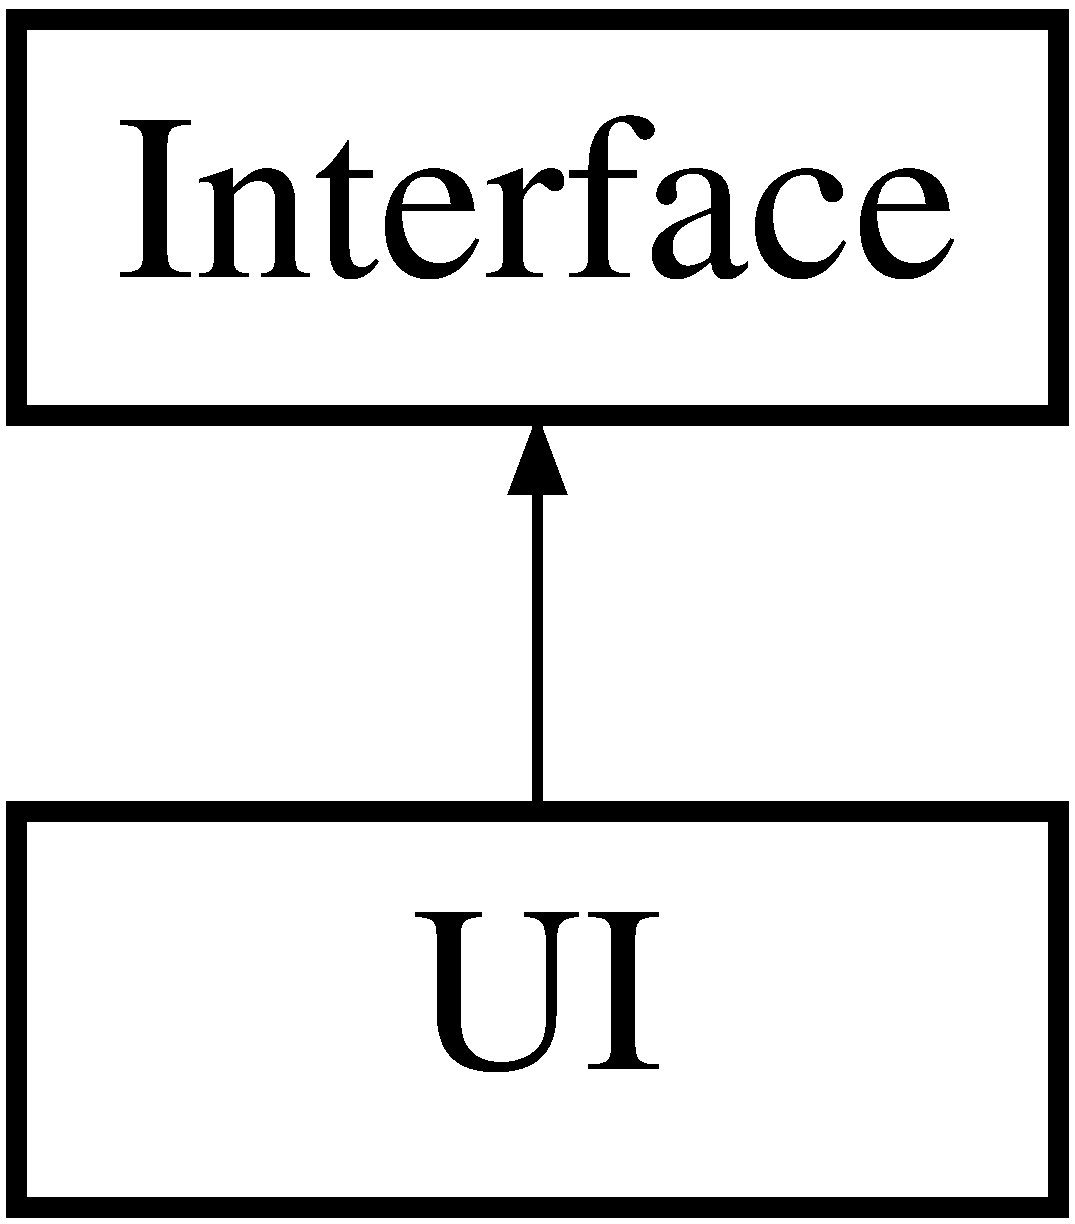
\includegraphics[height=2.000000cm]{class_interface}
\end{center}
\end{figure}
\subsection*{Public Member Functions}
\begin{DoxyCompactItemize}
\item 
\hyperlink{class_interface_a4406d74c75bdfe150bf72be1f1cda8b1}{Interface} ()
\item 
virtual \hyperlink{class_interface_a19179888f29f18f1be54a3dfe98f68c0}{$\sim$\+Interface} ()
\item 
void \hyperlink{class_interface_aeac0b572a2d73782b27da1f0084f0f5f}{Initialize} (const \hyperlink{class_render_window}{Render\+Window} \&active\+Window, bool instant\+Callbacks=true)
\item 
void \hyperlink{class_interface_a2bdcd6b2c85bb5f0bd756524a821b9df}{Terminate} ()
\item 
void \hyperlink{class_interface_a637ef08a4ccaaeedd10572470cf0afce}{Render} () const 
\item 
void \hyperlink{class_interface_ad7f4818ee9560b0462fc46ff82188413}{New\+Frame} ()
\end{DoxyCompactItemize}
\subsection*{Protected Member Functions}
\begin{DoxyCompactItemize}
\item 
virtual void \hyperlink{class_interface_a82df247fd022d924995421ab90444945}{Draw} ()=0
\end{DoxyCompactItemize}


\subsection{Detailed Description}


Definition at line 4 of file interface.\+h.



\subsection{Constructor \& Destructor Documentation}
\hypertarget{class_interface_a4406d74c75bdfe150bf72be1f1cda8b1}{}\index{Interface@{Interface}!Interface@{Interface}}
\index{Interface@{Interface}!Interface@{Interface}}
\subsubsection[{Interface()}]{\setlength{\rightskip}{0pt plus 5cm}Interface\+::\+Interface (
\begin{DoxyParamCaption}
{}
\end{DoxyParamCaption}
)}\label{class_interface_a4406d74c75bdfe150bf72be1f1cda8b1}


Definition at line 13 of file interface.\+cpp.

\hypertarget{class_interface_a19179888f29f18f1be54a3dfe98f68c0}{}\index{Interface@{Interface}!````~Interface@{$\sim$\+Interface}}
\index{````~Interface@{$\sim$\+Interface}!Interface@{Interface}}
\subsubsection[{$\sim$\+Interface()}]{\setlength{\rightskip}{0pt plus 5cm}Interface\+::$\sim$\+Interface (
\begin{DoxyParamCaption}
{}
\end{DoxyParamCaption}
)\hspace{0.3cm}{\ttfamily [virtual]}}\label{class_interface_a19179888f29f18f1be54a3dfe98f68c0}


Definition at line 18 of file interface.\+cpp.



\subsection{Member Function Documentation}
\hypertarget{class_interface_a82df247fd022d924995421ab90444945}{}\index{Interface@{Interface}!Draw@{Draw}}
\index{Draw@{Draw}!Interface@{Interface}}
\subsubsection[{Draw()=0}]{\setlength{\rightskip}{0pt plus 5cm}virtual void Interface\+::\+Draw (
\begin{DoxyParamCaption}
{}
\end{DoxyParamCaption}
)\hspace{0.3cm}{\ttfamily [protected]}, {\ttfamily [pure virtual]}}\label{class_interface_a82df247fd022d924995421ab90444945}


Implemented in \hyperlink{class_u_i_adb4cbcd5c39529f361c6543471e939a7}{U\+I}.

\hypertarget{class_interface_aeac0b572a2d73782b27da1f0084f0f5f}{}\index{Interface@{Interface}!Initialize@{Initialize}}
\index{Initialize@{Initialize}!Interface@{Interface}}
\subsubsection[{Initialize(const Render\+Window \&active\+Window, bool instant\+Callbacks=true)}]{\setlength{\rightskip}{0pt plus 5cm}void Interface\+::\+Initialize (
\begin{DoxyParamCaption}
\item[{const {\bf Render\+Window} \&}]{active\+Window, }
\item[{bool}]{instant\+Callbacks = {\ttfamily true}}
\end{DoxyParamCaption}
)}\label{class_interface_aeac0b572a2d73782b27da1f0084f0f5f}


Definition at line 130 of file interface.\+cpp.

\hypertarget{class_interface_ad7f4818ee9560b0462fc46ff82188413}{}\index{Interface@{Interface}!New\+Frame@{New\+Frame}}
\index{New\+Frame@{New\+Frame}!Interface@{Interface}}
\subsubsection[{New\+Frame()}]{\setlength{\rightskip}{0pt plus 5cm}void Interface\+::\+New\+Frame (
\begin{DoxyParamCaption}
{}
\end{DoxyParamCaption}
)}\label{class_interface_ad7f4818ee9560b0462fc46ff82188413}


Definition at line 179 of file interface.\+cpp.

\hypertarget{class_interface_a637ef08a4ccaaeedd10572470cf0afce}{}\index{Interface@{Interface}!Render@{Render}}
\index{Render@{Render}!Interface@{Interface}}
\subsubsection[{Render() const }]{\setlength{\rightskip}{0pt plus 5cm}void Interface\+::\+Render (
\begin{DoxyParamCaption}
{}
\end{DoxyParamCaption}
) const}\label{class_interface_a637ef08a4ccaaeedd10572470cf0afce}


Definition at line 174 of file interface.\+cpp.

\hypertarget{class_interface_a2bdcd6b2c85bb5f0bd756524a821b9df}{}\index{Interface@{Interface}!Terminate@{Terminate}}
\index{Terminate@{Terminate}!Interface@{Interface}}
\subsubsection[{Terminate()}]{\setlength{\rightskip}{0pt plus 5cm}void Interface\+::\+Terminate (
\begin{DoxyParamCaption}
{}
\end{DoxyParamCaption}
)}\label{class_interface_a2bdcd6b2c85bb5f0bd756524a821b9df}


Definition at line 341 of file interface.\+cpp.



The documentation for this class was generated from the following files\+:\begin{DoxyCompactItemize}
\item 
V\+C\+T\+\_\+\+Engine/interface/\hyperlink{interface_8h}{interface.\+h}\item 
V\+C\+T\+\_\+\+Engine/interface/\hyperlink{interface_8cpp}{interface.\+cpp}\end{DoxyCompactItemize}

\hypertarget{class_light}{}\section{Light Class Reference}
\label{class_light}\index{Light@{Light}}


{\ttfamily \#include $<$light.\+h$>$}

\subsection*{Public Types}
\begin{DoxyCompactItemize}
\item 
enum \hyperlink{class_light_a661d9480e01af8b1612860b9630ef5f8}{Light\+Type} \{ \hyperlink{class_light_a661d9480e01af8b1612860b9630ef5f8a65021ca49102cf10ed4bd541e828ab6f}{Disabled}, 
\hyperlink{class_light_a661d9480e01af8b1612860b9630ef5f8ae1a0035e4acfd2e430ed27b591db4433}{Directional}, 
\hyperlink{class_light_a661d9480e01af8b1612860b9630ef5f8a95beda1310e6c8e76384dc8e60986ec2}{Point}, 
\hyperlink{class_light_a661d9480e01af8b1612860b9630ef5f8a909d110309169cdae833f32e84b297bf}{Spot}
 \}
\end{DoxyCompactItemize}
\subsection*{Public Member Functions}
\begin{DoxyCompactItemize}
\item 
\hyperlink{class_light_aeb5df09a25a32f19fdffa761268ba24f}{Light} ()
\item 
\hyperlink{class_light_ad0e59fad13bb6cfadc25b2c477e9ddc7}{$\sim$\+Light} ()
\end{DoxyCompactItemize}
\subsection*{Public Attributes}
\begin{DoxyCompactItemize}
\item 
float \hyperlink{class_light_aaa42e1c80406d2703241bdda88819c7c}{angle\+Inner\+Cone}
\item 
float \hyperlink{class_light_a5bdec5d32c256ded1b7977b48c351ff3}{angle\+Outer\+Cone}
\item 
glm\+::vec3 \hyperlink{class_light_afaa34bb2efc167adcb2055359fd08a49}{ambient}
\item 
glm\+::vec3 \hyperlink{class_light_ad47b5347556fd8cd9ebdc60fdfed196b}{diffuse}
\item 
glm\+::vec3 \hyperlink{class_light_aefcfb83a0540ddb885c2622061b28d7e}{specular}
\item 
glm\+::vec3 \hyperlink{class_light_a494230a45b5cfa2f9fb54dbd4de3812b}{direction}
\item 
glm\+::vec3 \hyperlink{class_light_a89bffe071ec6431a21c5b54021fe08d6}{position}
\item 
\hyperlink{struct_attenuation}{Attenuation} \hyperlink{class_light_a6684545092d9a9b80422a6612e5cac26}{attenuation}
\item 
\hyperlink{class_light_a661d9480e01af8b1612860b9630ef5f8}{Light\+Type} \hyperlink{class_light_ab0c279c927973443f7b52fc924b489aa}{light\+Type}
\end{DoxyCompactItemize}


\subsection{Detailed Description}


Definition at line 12 of file light.\+h.



\subsection{Member Enumeration Documentation}
\hypertarget{class_light_a661d9480e01af8b1612860b9630ef5f8}{}\index{Light@{Light}!Light\+Type@{Light\+Type}}
\index{Light\+Type@{Light\+Type}!Light@{Light}}
\subsubsection[{Light\+Type}]{\setlength{\rightskip}{0pt plus 5cm}enum {\bf Light\+::\+Light\+Type}}\label{class_light_a661d9480e01af8b1612860b9630ef5f8}
\begin{Desc}
\item[Enumerator]\par
\begin{description}
\index{Disabled@{Disabled}!Light@{Light}}\index{Light@{Light}!Disabled@{Disabled}}\item[{\em 
\hypertarget{class_light_a661d9480e01af8b1612860b9630ef5f8a65021ca49102cf10ed4bd541e828ab6f}{}Disabled\label{class_light_a661d9480e01af8b1612860b9630ef5f8a65021ca49102cf10ed4bd541e828ab6f}
}]\index{Directional@{Directional}!Light@{Light}}\index{Light@{Light}!Directional@{Directional}}\item[{\em 
\hypertarget{class_light_a661d9480e01af8b1612860b9630ef5f8ae1a0035e4acfd2e430ed27b591db4433}{}Directional\label{class_light_a661d9480e01af8b1612860b9630ef5f8ae1a0035e4acfd2e430ed27b591db4433}
}]\index{Point@{Point}!Light@{Light}}\index{Light@{Light}!Point@{Point}}\item[{\em 
\hypertarget{class_light_a661d9480e01af8b1612860b9630ef5f8a95beda1310e6c8e76384dc8e60986ec2}{}Point\label{class_light_a661d9480e01af8b1612860b9630ef5f8a95beda1310e6c8e76384dc8e60986ec2}
}]\index{Spot@{Spot}!Light@{Light}}\index{Light@{Light}!Spot@{Spot}}\item[{\em 
\hypertarget{class_light_a661d9480e01af8b1612860b9630ef5f8a909d110309169cdae833f32e84b297bf}{}Spot\label{class_light_a661d9480e01af8b1612860b9630ef5f8a909d110309169cdae833f32e84b297bf}
}]\end{description}
\end{Desc}


Definition at line 15 of file light.\+h.



\subsection{Constructor \& Destructor Documentation}
\hypertarget{class_light_aeb5df09a25a32f19fdffa761268ba24f}{}\index{Light@{Light}!Light@{Light}}
\index{Light@{Light}!Light@{Light}}
\subsubsection[{Light()}]{\setlength{\rightskip}{0pt plus 5cm}Light\+::\+Light (
\begin{DoxyParamCaption}
{}
\end{DoxyParamCaption}
)}\label{class_light_aeb5df09a25a32f19fdffa761268ba24f}


Definition at line 5 of file light.\+cpp.

\hypertarget{class_light_ad0e59fad13bb6cfadc25b2c477e9ddc7}{}\index{Light@{Light}!````~Light@{$\sim$\+Light}}
\index{````~Light@{$\sim$\+Light}!Light@{Light}}
\subsubsection[{$\sim$\+Light()}]{\setlength{\rightskip}{0pt plus 5cm}Light\+::$\sim$\+Light (
\begin{DoxyParamCaption}
{}
\end{DoxyParamCaption}
)}\label{class_light_ad0e59fad13bb6cfadc25b2c477e9ddc7}


Definition at line 13 of file light.\+cpp.



\subsection{Member Data Documentation}
\hypertarget{class_light_afaa34bb2efc167adcb2055359fd08a49}{}\index{Light@{Light}!ambient@{ambient}}
\index{ambient@{ambient}!Light@{Light}}
\subsubsection[{ambient}]{\setlength{\rightskip}{0pt plus 5cm}glm\+::vec3 Light\+::ambient}\label{class_light_afaa34bb2efc167adcb2055359fd08a49}


Definition at line 26 of file light.\+h.

\hypertarget{class_light_aaa42e1c80406d2703241bdda88819c7c}{}\index{Light@{Light}!angle\+Inner\+Cone@{angle\+Inner\+Cone}}
\index{angle\+Inner\+Cone@{angle\+Inner\+Cone}!Light@{Light}}
\subsubsection[{angle\+Inner\+Cone}]{\setlength{\rightskip}{0pt plus 5cm}float Light\+::angle\+Inner\+Cone}\label{class_light_aaa42e1c80406d2703241bdda88819c7c}


Definition at line 23 of file light.\+h.

\hypertarget{class_light_a5bdec5d32c256ded1b7977b48c351ff3}{}\index{Light@{Light}!angle\+Outer\+Cone@{angle\+Outer\+Cone}}
\index{angle\+Outer\+Cone@{angle\+Outer\+Cone}!Light@{Light}}
\subsubsection[{angle\+Outer\+Cone}]{\setlength{\rightskip}{0pt plus 5cm}float Light\+::angle\+Outer\+Cone}\label{class_light_a5bdec5d32c256ded1b7977b48c351ff3}


Definition at line 24 of file light.\+h.

\hypertarget{class_light_a6684545092d9a9b80422a6612e5cac26}{}\index{Light@{Light}!attenuation@{attenuation}}
\index{attenuation@{attenuation}!Light@{Light}}
\subsubsection[{attenuation}]{\setlength{\rightskip}{0pt plus 5cm}{\bf Attenuation} Light\+::attenuation}\label{class_light_a6684545092d9a9b80422a6612e5cac26}


Definition at line 33 of file light.\+h.

\hypertarget{class_light_ad47b5347556fd8cd9ebdc60fdfed196b}{}\index{Light@{Light}!diffuse@{diffuse}}
\index{diffuse@{diffuse}!Light@{Light}}
\subsubsection[{diffuse}]{\setlength{\rightskip}{0pt plus 5cm}glm\+::vec3 Light\+::diffuse}\label{class_light_ad47b5347556fd8cd9ebdc60fdfed196b}


Definition at line 27 of file light.\+h.

\hypertarget{class_light_a494230a45b5cfa2f9fb54dbd4de3812b}{}\index{Light@{Light}!direction@{direction}}
\index{direction@{direction}!Light@{Light}}
\subsubsection[{direction}]{\setlength{\rightskip}{0pt plus 5cm}glm\+::vec3 Light\+::direction}\label{class_light_a494230a45b5cfa2f9fb54dbd4de3812b}


Definition at line 30 of file light.\+h.

\hypertarget{class_light_ab0c279c927973443f7b52fc924b489aa}{}\index{Light@{Light}!light\+Type@{light\+Type}}
\index{light\+Type@{light\+Type}!Light@{Light}}
\subsubsection[{light\+Type}]{\setlength{\rightskip}{0pt plus 5cm}{\bf Light\+Type} Light\+::light\+Type}\label{class_light_ab0c279c927973443f7b52fc924b489aa}


Definition at line 35 of file light.\+h.

\hypertarget{class_light_a89bffe071ec6431a21c5b54021fe08d6}{}\index{Light@{Light}!position@{position}}
\index{position@{position}!Light@{Light}}
\subsubsection[{position}]{\setlength{\rightskip}{0pt plus 5cm}glm\+::vec3 Light\+::position}\label{class_light_a89bffe071ec6431a21c5b54021fe08d6}


Definition at line 31 of file light.\+h.

\hypertarget{class_light_aefcfb83a0540ddb885c2622061b28d7e}{}\index{Light@{Light}!specular@{specular}}
\index{specular@{specular}!Light@{Light}}
\subsubsection[{specular}]{\setlength{\rightskip}{0pt plus 5cm}glm\+::vec3 Light\+::specular}\label{class_light_aefcfb83a0540ddb885c2622061b28d7e}


Definition at line 28 of file light.\+h.



The documentation for this class was generated from the following files\+:\begin{DoxyCompactItemize}
\item 
V\+C\+T\+\_\+\+Engine/scene/\hyperlink{light_8h}{light.\+h}\item 
V\+C\+T\+\_\+\+Engine/scene/\hyperlink{light_8cpp}{light.\+cpp}\end{DoxyCompactItemize}

\hypertarget{class_material}{}\section{Material Class Reference}
\label{class_material}\index{Material@{Material}}


{\ttfamily \#include $<$material.\+h$>$}

Inheritance diagram for Material\+:\begin{figure}[H]
\begin{center}
\leavevmode
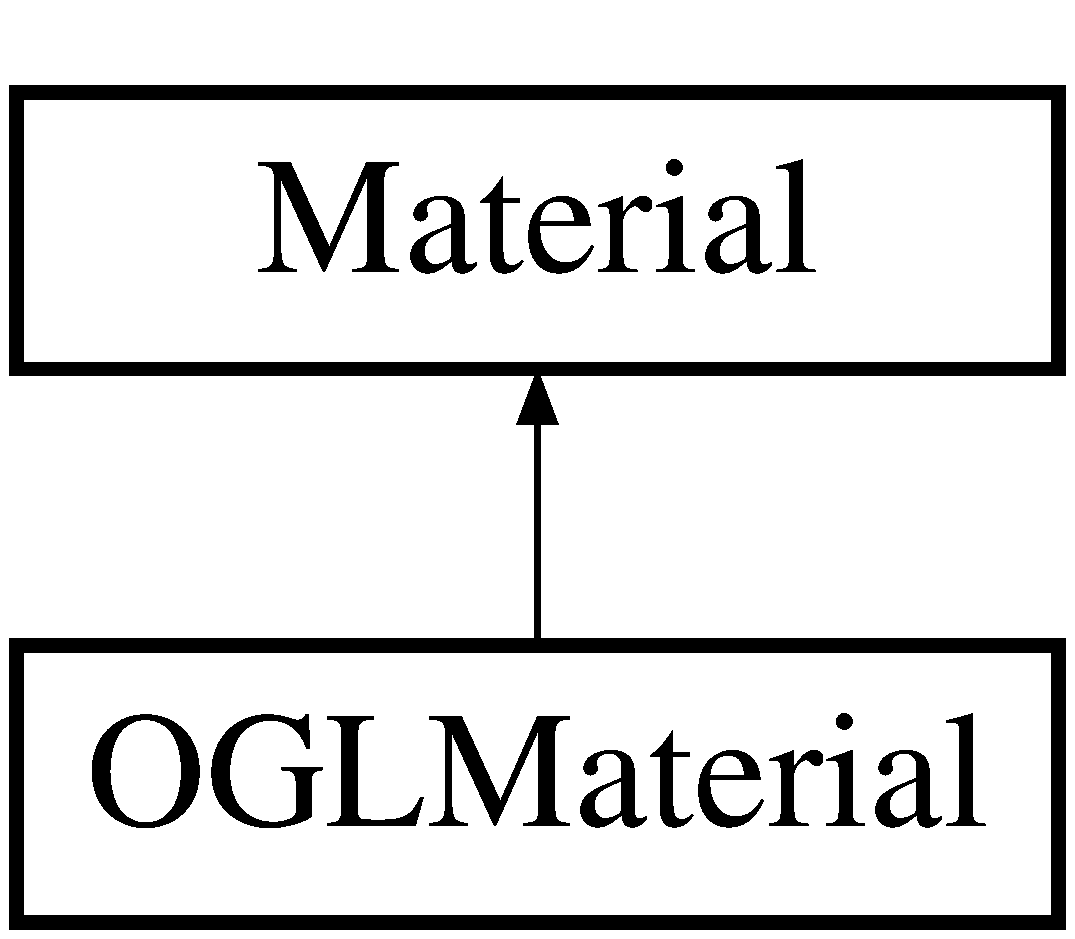
\includegraphics[height=2.000000cm]{class_material}
\end{center}
\end{figure}
\subsection*{Public Attributes}
\begin{DoxyCompactItemize}
\item 
glm\+::vec3 \hyperlink{class_material_af99c823542e497c98a35d1aac5fc9012}{ambient}
\item 
glm\+::vec3 \hyperlink{class_material_a099904e2f5a7bbec3cba6bf8ec546b11}{diffuse}
\item 
glm\+::vec3 \hyperlink{class_material_aac1c499923ff99564cdd97a4b5e504a9}{specular}
\item 
glm\+::vec3 \hyperlink{class_material_ab35396b9c5340ce4a785884c54fbe2ac}{emissive}
\item 
glm\+::vec3 \hyperlink{class_material_ad65e6df916690d7a2e59d18ec3f25c1c}{transparent}
\item 
float \hyperlink{class_material_a4ddb4745b69e0b8747ef819bc3e3ceee}{opacity}
\item 
float \hyperlink{class_material_a9dc184c883ec135ace28c1917af3fe84}{shininess}
\item 
float \hyperlink{class_material_a39204190f2a9ff5e1d3ff8f109c97d67}{shininess\+Strenght}
\item 
float \hyperlink{class_material_a52b96d96f3a3c9bf506fd7dc7ff6f40a}{refraction\+Index}
\item 
unsigned int \hyperlink{class_material_a86b8ac102b9af92d5bc715efd4068a91}{material\+Flags}
\end{DoxyCompactItemize}


\subsection{Detailed Description}


Definition at line 4 of file material.\+h.



\subsection{Member Data Documentation}
\hypertarget{class_material_af99c823542e497c98a35d1aac5fc9012}{}\index{Material@{Material}!ambient@{ambient}}
\index{ambient@{ambient}!Material@{Material}}
\subsubsection[{ambient}]{\setlength{\rightskip}{0pt plus 5cm}glm\+::vec3 Material\+::ambient}\label{class_material_af99c823542e497c98a35d1aac5fc9012}


Definition at line 7 of file material.\+h.

\hypertarget{class_material_a099904e2f5a7bbec3cba6bf8ec546b11}{}\index{Material@{Material}!diffuse@{diffuse}}
\index{diffuse@{diffuse}!Material@{Material}}
\subsubsection[{diffuse}]{\setlength{\rightskip}{0pt plus 5cm}glm\+::vec3 Material\+::diffuse}\label{class_material_a099904e2f5a7bbec3cba6bf8ec546b11}


Definition at line 8 of file material.\+h.

\hypertarget{class_material_ab35396b9c5340ce4a785884c54fbe2ac}{}\index{Material@{Material}!emissive@{emissive}}
\index{emissive@{emissive}!Material@{Material}}
\subsubsection[{emissive}]{\setlength{\rightskip}{0pt plus 5cm}glm\+::vec3 Material\+::emissive}\label{class_material_ab35396b9c5340ce4a785884c54fbe2ac}


Definition at line 10 of file material.\+h.

\hypertarget{class_material_a86b8ac102b9af92d5bc715efd4068a91}{}\index{Material@{Material}!material\+Flags@{material\+Flags}}
\index{material\+Flags@{material\+Flags}!Material@{Material}}
\subsubsection[{material\+Flags}]{\setlength{\rightskip}{0pt plus 5cm}unsigned int Material\+::material\+Flags}\label{class_material_a86b8ac102b9af92d5bc715efd4068a91}


Definition at line 18 of file material.\+h.

\hypertarget{class_material_a4ddb4745b69e0b8747ef819bc3e3ceee}{}\index{Material@{Material}!opacity@{opacity}}
\index{opacity@{opacity}!Material@{Material}}
\subsubsection[{opacity}]{\setlength{\rightskip}{0pt plus 5cm}float Material\+::opacity}\label{class_material_a4ddb4745b69e0b8747ef819bc3e3ceee}


Definition at line 13 of file material.\+h.

\hypertarget{class_material_a52b96d96f3a3c9bf506fd7dc7ff6f40a}{}\index{Material@{Material}!refraction\+Index@{refraction\+Index}}
\index{refraction\+Index@{refraction\+Index}!Material@{Material}}
\subsubsection[{refraction\+Index}]{\setlength{\rightskip}{0pt plus 5cm}float Material\+::refraction\+Index}\label{class_material_a52b96d96f3a3c9bf506fd7dc7ff6f40a}


Definition at line 16 of file material.\+h.

\hypertarget{class_material_a9dc184c883ec135ace28c1917af3fe84}{}\index{Material@{Material}!shininess@{shininess}}
\index{shininess@{shininess}!Material@{Material}}
\subsubsection[{shininess}]{\setlength{\rightskip}{0pt plus 5cm}float Material\+::shininess}\label{class_material_a9dc184c883ec135ace28c1917af3fe84}


Definition at line 14 of file material.\+h.

\hypertarget{class_material_a39204190f2a9ff5e1d3ff8f109c97d67}{}\index{Material@{Material}!shininess\+Strenght@{shininess\+Strenght}}
\index{shininess\+Strenght@{shininess\+Strenght}!Material@{Material}}
\subsubsection[{shininess\+Strenght}]{\setlength{\rightskip}{0pt plus 5cm}float Material\+::shininess\+Strenght}\label{class_material_a39204190f2a9ff5e1d3ff8f109c97d67}


Definition at line 15 of file material.\+h.

\hypertarget{class_material_aac1c499923ff99564cdd97a4b5e504a9}{}\index{Material@{Material}!specular@{specular}}
\index{specular@{specular}!Material@{Material}}
\subsubsection[{specular}]{\setlength{\rightskip}{0pt plus 5cm}glm\+::vec3 Material\+::specular}\label{class_material_aac1c499923ff99564cdd97a4b5e504a9}


Definition at line 9 of file material.\+h.

\hypertarget{class_material_ad65e6df916690d7a2e59d18ec3f25c1c}{}\index{Material@{Material}!transparent@{transparent}}
\index{transparent@{transparent}!Material@{Material}}
\subsubsection[{transparent}]{\setlength{\rightskip}{0pt plus 5cm}glm\+::vec3 Material\+::transparent}\label{class_material_ad65e6df916690d7a2e59d18ec3f25c1c}


Definition at line 11 of file material.\+h.



The documentation for this class was generated from the following file\+:\begin{DoxyCompactItemize}
\item 
V\+C\+T\+\_\+\+Engine/scene/\hyperlink{material_8h}{material.\+h}\end{DoxyCompactItemize}

\hypertarget{struct_matrices}{}\section{Matrices Struct Reference}
\label{struct_matrices}\index{Matrices@{Matrices}}


{\ttfamily \#include $<$transform\+\_\+matrices.\+h$>$}

\subsection*{Public Attributes}
\begin{DoxyCompactItemize}
\item 
glm\+::mat4x4 \hyperlink{struct_matrices_a55eeaf59b817be66d2149f5e131f8de3}{model\+View}
\item 
glm\+::mat4x4 \hyperlink{struct_matrices_a42af8cc09c21dbba6c3284291d2dba61}{model\+View\+Projection}
\item 
glm\+::mat4x4 \hyperlink{struct_matrices_af7523266e69ac370269472837fd6cacf}{model}
\item 
glm\+::mat4x4 \hyperlink{struct_matrices_af1345e145e678b3430cb794fb25b86ce}{view}
\item 
glm\+::mat4x4 \hyperlink{struct_matrices_a39c06d4402c7e41b394a74790934fc53}{projection}
\item 
glm\+::mat4x4 \hyperlink{struct_matrices_ae02f038cdeb0852e4235ab59d111337e}{normal}
\end{DoxyCompactItemize}


\subsection{Detailed Description}


Definition at line 4 of file transform\+\_\+matrices.\+h.



\subsection{Member Data Documentation}
\hypertarget{struct_matrices_af7523266e69ac370269472837fd6cacf}{}\index{Matrices@{Matrices}!model@{model}}
\index{model@{model}!Matrices@{Matrices}}
\subsubsection[{model}]{\setlength{\rightskip}{0pt plus 5cm}glm\+::mat4x4 Matrices\+::model}\label{struct_matrices_af7523266e69ac370269472837fd6cacf}


Definition at line 8 of file transform\+\_\+matrices.\+h.

\hypertarget{struct_matrices_a55eeaf59b817be66d2149f5e131f8de3}{}\index{Matrices@{Matrices}!model\+View@{model\+View}}
\index{model\+View@{model\+View}!Matrices@{Matrices}}
\subsubsection[{model\+View}]{\setlength{\rightskip}{0pt plus 5cm}glm\+::mat4x4 Matrices\+::model\+View}\label{struct_matrices_a55eeaf59b817be66d2149f5e131f8de3}


Definition at line 6 of file transform\+\_\+matrices.\+h.

\hypertarget{struct_matrices_a42af8cc09c21dbba6c3284291d2dba61}{}\index{Matrices@{Matrices}!model\+View\+Projection@{model\+View\+Projection}}
\index{model\+View\+Projection@{model\+View\+Projection}!Matrices@{Matrices}}
\subsubsection[{model\+View\+Projection}]{\setlength{\rightskip}{0pt plus 5cm}glm\+::mat4x4 Matrices\+::model\+View\+Projection}\label{struct_matrices_a42af8cc09c21dbba6c3284291d2dba61}


Definition at line 7 of file transform\+\_\+matrices.\+h.

\hypertarget{struct_matrices_ae02f038cdeb0852e4235ab59d111337e}{}\index{Matrices@{Matrices}!normal@{normal}}
\index{normal@{normal}!Matrices@{Matrices}}
\subsubsection[{normal}]{\setlength{\rightskip}{0pt plus 5cm}glm\+::mat4x4 Matrices\+::normal}\label{struct_matrices_ae02f038cdeb0852e4235ab59d111337e}


Definition at line 11 of file transform\+\_\+matrices.\+h.

\hypertarget{struct_matrices_a39c06d4402c7e41b394a74790934fc53}{}\index{Matrices@{Matrices}!projection@{projection}}
\index{projection@{projection}!Matrices@{Matrices}}
\subsubsection[{projection}]{\setlength{\rightskip}{0pt plus 5cm}glm\+::mat4x4 Matrices\+::projection}\label{struct_matrices_a39c06d4402c7e41b394a74790934fc53}


Definition at line 10 of file transform\+\_\+matrices.\+h.

\hypertarget{struct_matrices_af1345e145e678b3430cb794fb25b86ce}{}\index{Matrices@{Matrices}!view@{view}}
\index{view@{view}!Matrices@{Matrices}}
\subsubsection[{view}]{\setlength{\rightskip}{0pt plus 5cm}glm\+::mat4x4 Matrices\+::view}\label{struct_matrices_af1345e145e678b3430cb794fb25b86ce}


Definition at line 9 of file transform\+\_\+matrices.\+h.



The documentation for this struct was generated from the following file\+:\begin{DoxyCompactItemize}
\item 
V\+C\+T\+\_\+\+Engine/types/\hyperlink{transform__matrices_8h}{transform\+\_\+matrices.\+h}\end{DoxyCompactItemize}

\hypertarget{class_mesh}{}\section{Mesh Class Reference}
\label{class_mesh}\index{Mesh@{Mesh}}


{\ttfamily \#include $<$mesh.\+h$>$}

Inheritance diagram for Mesh\+:\begin{figure}[H]
\begin{center}
\leavevmode
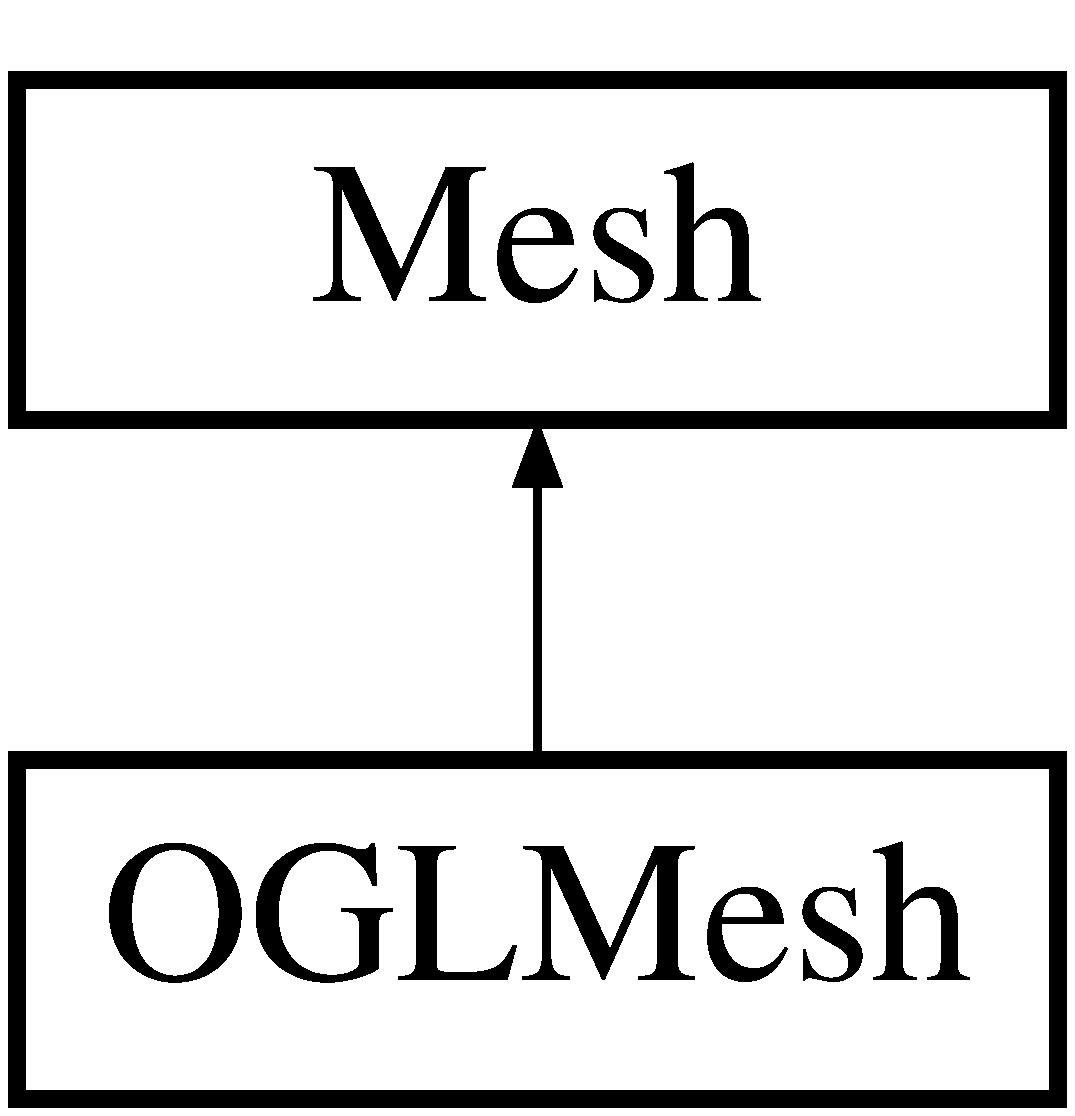
\includegraphics[height=2.000000cm]{class_mesh}
\end{center}
\end{figure}
\subsection*{Public Member Functions}
\begin{DoxyCompactItemize}
\item 
\hyperlink{class_mesh_a2af137f1571af89172b9c102302c416b}{Mesh} ()
\item 
virtual \hyperlink{class_mesh_a5efe4da1a4c0971cfb037bd70304c303}{$\sim$\+Mesh} ()
\item 
void \hyperlink{class_mesh_ae89fa54cbcdae224c00bbe5501ac2f05}{Free\+Raw\+Data} ()
\end{DoxyCompactItemize}
\subsection*{Public Attributes}
\begin{DoxyCompactItemize}
\item 
\hyperlink{class_bounding_volume}{Bounding\+Volume} \hyperlink{class_mesh_af058fb0d0fd3933311a4a05621ec95f7}{boundaries}
\item 
std\+::string \hyperlink{class_mesh_ac687e9dcfc7cc60b046fc2ec634200be}{name}
\item 
std\+::vector$<$ \hyperlink{struct_vertex}{Vertex} $>$ \hyperlink{class_mesh_a6465a888c97232a39e12aad008c969c3}{vertices}
\item 
std\+::vector$<$ unsigned int $>$ \hyperlink{class_mesh_a26632e27b772f24b069a738e7983b9da}{indices}
\item 
std\+::shared\+\_\+ptr$<$ \hyperlink{class_o_g_l_material}{O\+G\+L\+Material} $>$ \hyperlink{class_mesh_ae392f8f4565054b3ef98ab2d41f86cc9}{material}
\end{DoxyCompactItemize}


\subsection{Detailed Description}


Definition at line 6 of file mesh.\+h.



\subsection{Constructor \& Destructor Documentation}
\hypertarget{class_mesh_a2af137f1571af89172b9c102302c416b}{}\index{Mesh@{Mesh}!Mesh@{Mesh}}
\index{Mesh@{Mesh}!Mesh@{Mesh}}
\subsubsection[{Mesh()}]{\setlength{\rightskip}{0pt plus 5cm}Mesh\+::\+Mesh (
\begin{DoxyParamCaption}
{}
\end{DoxyParamCaption}
)}\label{class_mesh_a2af137f1571af89172b9c102302c416b}


Definition at line 5 of file mesh.\+cpp.

\hypertarget{class_mesh_a5efe4da1a4c0971cfb037bd70304c303}{}\index{Mesh@{Mesh}!````~Mesh@{$\sim$\+Mesh}}
\index{````~Mesh@{$\sim$\+Mesh}!Mesh@{Mesh}}
\subsubsection[{$\sim$\+Mesh()}]{\setlength{\rightskip}{0pt plus 5cm}Mesh\+::$\sim$\+Mesh (
\begin{DoxyParamCaption}
{}
\end{DoxyParamCaption}
)\hspace{0.3cm}{\ttfamily [virtual]}}\label{class_mesh_a5efe4da1a4c0971cfb037bd70304c303}


Definition at line 10 of file mesh.\+cpp.



\subsection{Member Function Documentation}
\hypertarget{class_mesh_ae89fa54cbcdae224c00bbe5501ac2f05}{}\index{Mesh@{Mesh}!Free\+Raw\+Data@{Free\+Raw\+Data}}
\index{Free\+Raw\+Data@{Free\+Raw\+Data}!Mesh@{Mesh}}
\subsubsection[{Free\+Raw\+Data()}]{\setlength{\rightskip}{0pt plus 5cm}void Mesh\+::\+Free\+Raw\+Data (
\begin{DoxyParamCaption}
{}
\end{DoxyParamCaption}
)}\label{class_mesh_ae89fa54cbcdae224c00bbe5501ac2f05}


Definition at line 14 of file mesh.\+cpp.



\subsection{Member Data Documentation}
\hypertarget{class_mesh_af058fb0d0fd3933311a4a05621ec95f7}{}\index{Mesh@{Mesh}!boundaries@{boundaries}}
\index{boundaries@{boundaries}!Mesh@{Mesh}}
\subsubsection[{boundaries}]{\setlength{\rightskip}{0pt plus 5cm}{\bf Bounding\+Volume} Mesh\+::boundaries}\label{class_mesh_af058fb0d0fd3933311a4a05621ec95f7}


Definition at line 11 of file mesh.\+h.

\hypertarget{class_mesh_a26632e27b772f24b069a738e7983b9da}{}\index{Mesh@{Mesh}!indices@{indices}}
\index{indices@{indices}!Mesh@{Mesh}}
\subsubsection[{indices}]{\setlength{\rightskip}{0pt plus 5cm}std\+::vector$<$unsigned int$>$ Mesh\+::indices}\label{class_mesh_a26632e27b772f24b069a738e7983b9da}


Definition at line 16 of file mesh.\+h.

\hypertarget{class_mesh_ae392f8f4565054b3ef98ab2d41f86cc9}{}\index{Mesh@{Mesh}!material@{material}}
\index{material@{material}!Mesh@{Mesh}}
\subsubsection[{material}]{\setlength{\rightskip}{0pt plus 5cm}std\+::shared\+\_\+ptr$<${\bf O\+G\+L\+Material}$>$ Mesh\+::material}\label{class_mesh_ae392f8f4565054b3ef98ab2d41f86cc9}


Definition at line 18 of file mesh.\+h.

\hypertarget{class_mesh_ac687e9dcfc7cc60b046fc2ec634200be}{}\index{Mesh@{Mesh}!name@{name}}
\index{name@{name}!Mesh@{Mesh}}
\subsubsection[{name}]{\setlength{\rightskip}{0pt plus 5cm}std\+::string Mesh\+::name}\label{class_mesh_ac687e9dcfc7cc60b046fc2ec634200be}


Definition at line 13 of file mesh.\+h.

\hypertarget{class_mesh_a6465a888c97232a39e12aad008c969c3}{}\index{Mesh@{Mesh}!vertices@{vertices}}
\index{vertices@{vertices}!Mesh@{Mesh}}
\subsubsection[{vertices}]{\setlength{\rightskip}{0pt plus 5cm}std\+::vector$<${\bf Vertex}$>$ Mesh\+::vertices}\label{class_mesh_a6465a888c97232a39e12aad008c969c3}


Definition at line 15 of file mesh.\+h.



The documentation for this class was generated from the following files\+:\begin{DoxyCompactItemize}
\item 
V\+C\+T\+\_\+\+Engine/scene/\hyperlink{mesh_8h}{mesh.\+h}\item 
V\+C\+T\+\_\+\+Engine/scene/\hyperlink{mesh_8cpp}{mesh.\+cpp}\end{DoxyCompactItemize}

\hypertarget{class_node}{}\section{Node Class Reference}
\label{class_node}\index{Node@{Node}}


{\ttfamily \#include $<$node.\+h$>$}

\subsection*{Public Member Functions}
\begin{DoxyCompactItemize}
\item 
\hyperlink{class_node_ad7a34779cad45d997bfd6d3d8043c75f}{Node} ()
\item 
virtual \hyperlink{class_node_aa0840c3cb5c7159be6d992adecd2097c}{$\sim$\+Node} ()
\item 
glm\+::mat4x4 \hyperlink{class_node_a7b521faa617ff77270c0b2bf2d5ab02d}{Get\+Model\+Matrix} () const 
\item 
void \hyperlink{class_node_afc101c74031fcbff9015bf79aea3ca0f}{Recalculate\+Model\+Matrix} ()
\item 
void \hyperlink{class_node_a0f2c6c5592597dd219aa64a1ab2814ee}{Draw} ()
\item 
void \hyperlink{class_node_ac793b348724a24608d3ea2b96b1a074e}{Draw\+Recursive} ()
\item 
void \hyperlink{class_node_aaf9201473c09c0e6e303438b1f9d5e3e}{Draw\+Meshes} ()
\item 
void \hyperlink{class_node_ae955f587b5f1efc7636eb895f7dfa146}{Transform} (const glm\+::vec3 \&position, const glm\+::vec3 \&scaling, const glm\+::quat \&rotation)
\item 
void \hyperlink{class_node_a80b0801a8f5ed09d8f00efab99aadb71}{Position} (const glm\+::vec3 \&position)
\item 
void \hyperlink{class_node_af830cf6546989912a102da44bb1533d1}{Scaling} (const glm\+::vec3 \&scaling)
\item 
void \hyperlink{class_node_a0a512a21da4f181ffa2df9ae7f3e1fd0}{Rotation} (const glm\+::quat \&rotation)
\end{DoxyCompactItemize}
\subsection*{Public Attributes}
\begin{DoxyCompactItemize}
\item 
\hyperlink{class_bounding_volume}{Bounding\+Volume} \hyperlink{class_node_a15ee4828bc458d3f697ac05d8b89629e}{boundaries}
\item 
std\+::string \hyperlink{class_node_aa829edc37a2c92dacdab95bcef248175}{name}
\item 
std\+::vector$<$ std\+::shared\+\_\+ptr$<$ \hyperlink{class_o_g_l_mesh}{O\+G\+L\+Mesh} $>$ $>$ \hyperlink{class_node_a79c7e73aae4df0de7d3941bb0ecf21eb}{meshes}
\item 
std\+::vector$<$ \hyperlink{class_node}{Node} $>$ \hyperlink{class_node_a34418a952053ee6d9884174e86054e8b}{nodes}
\end{DoxyCompactItemize}


\subsection{Detailed Description}


Definition at line 4 of file node.\+h.



\subsection{Constructor \& Destructor Documentation}
\hypertarget{class_node_ad7a34779cad45d997bfd6d3d8043c75f}{}\index{Node@{Node}!Node@{Node}}
\index{Node@{Node}!Node@{Node}}
\subsubsection[{Node()}]{\setlength{\rightskip}{0pt plus 5cm}Node\+::\+Node (
\begin{DoxyParamCaption}
{}
\end{DoxyParamCaption}
)}\label{class_node_ad7a34779cad45d997bfd6d3d8043c75f}


Definition at line 6 of file node.\+cpp.

\hypertarget{class_node_aa0840c3cb5c7159be6d992adecd2097c}{}\index{Node@{Node}!````~Node@{$\sim$\+Node}}
\index{````~Node@{$\sim$\+Node}!Node@{Node}}
\subsubsection[{$\sim$\+Node()}]{\setlength{\rightskip}{0pt plus 5cm}Node\+::$\sim$\+Node (
\begin{DoxyParamCaption}
{}
\end{DoxyParamCaption}
)\hspace{0.3cm}{\ttfamily [virtual]}}\label{class_node_aa0840c3cb5c7159be6d992adecd2097c}


Definition at line 16 of file node.\+cpp.



\subsection{Member Function Documentation}
\hypertarget{class_node_a0f2c6c5592597dd219aa64a1ab2814ee}{}\index{Node@{Node}!Draw@{Draw}}
\index{Draw@{Draw}!Node@{Node}}
\subsubsection[{Draw()}]{\setlength{\rightskip}{0pt plus 5cm}void Node\+::\+Draw (
\begin{DoxyParamCaption}
{}
\end{DoxyParamCaption}
)}\label{class_node_a0f2c6c5592597dd219aa64a1ab2814ee}


Definition at line 58 of file node.\+cpp.

\hypertarget{class_node_aaf9201473c09c0e6e303438b1f9d5e3e}{}\index{Node@{Node}!Draw\+Meshes@{Draw\+Meshes}}
\index{Draw\+Meshes@{Draw\+Meshes}!Node@{Node}}
\subsubsection[{Draw\+Meshes()}]{\setlength{\rightskip}{0pt plus 5cm}void Node\+::\+Draw\+Meshes (
\begin{DoxyParamCaption}
{}
\end{DoxyParamCaption}
)}\label{class_node_aaf9201473c09c0e6e303438b1f9d5e3e}


Definition at line 36 of file node.\+cpp.

\hypertarget{class_node_ac793b348724a24608d3ea2b96b1a074e}{}\index{Node@{Node}!Draw\+Recursive@{Draw\+Recursive}}
\index{Draw\+Recursive@{Draw\+Recursive}!Node@{Node}}
\subsubsection[{Draw\+Recursive()}]{\setlength{\rightskip}{0pt plus 5cm}void Node\+::\+Draw\+Recursive (
\begin{DoxyParamCaption}
{}
\end{DoxyParamCaption}
)}\label{class_node_ac793b348724a24608d3ea2b96b1a074e}


Definition at line 79 of file node.\+cpp.

\hypertarget{class_node_a7b521faa617ff77270c0b2bf2d5ab02d}{}\index{Node@{Node}!Get\+Model\+Matrix@{Get\+Model\+Matrix}}
\index{Get\+Model\+Matrix@{Get\+Model\+Matrix}!Node@{Node}}
\subsubsection[{Get\+Model\+Matrix() const }]{\setlength{\rightskip}{0pt plus 5cm}glm\+::mat4x4 Node\+::\+Get\+Model\+Matrix (
\begin{DoxyParamCaption}
{}
\end{DoxyParamCaption}
) const}\label{class_node_a7b521faa617ff77270c0b2bf2d5ab02d}


Definition at line 20 of file node.\+cpp.

\hypertarget{class_node_a80b0801a8f5ed09d8f00efab99aadb71}{}\index{Node@{Node}!Position@{Position}}
\index{Position@{Position}!Node@{Node}}
\subsubsection[{Position(const glm\+::vec3 \&position)}]{\setlength{\rightskip}{0pt plus 5cm}void Node\+::\+Position (
\begin{DoxyParamCaption}
\item[{const glm\+::vec3 \&}]{position}
\end{DoxyParamCaption}
)}\label{class_node_a80b0801a8f5ed09d8f00efab99aadb71}


Definition at line 118 of file node.\+cpp.

\hypertarget{class_node_afc101c74031fcbff9015bf79aea3ca0f}{}\index{Node@{Node}!Recalculate\+Model\+Matrix@{Recalculate\+Model\+Matrix}}
\index{Recalculate\+Model\+Matrix@{Recalculate\+Model\+Matrix}!Node@{Node}}
\subsubsection[{Recalculate\+Model\+Matrix()}]{\setlength{\rightskip}{0pt plus 5cm}void Node\+::\+Recalculate\+Model\+Matrix (
\begin{DoxyParamCaption}
{}
\end{DoxyParamCaption}
)}\label{class_node_afc101c74031fcbff9015bf79aea3ca0f}


Definition at line 25 of file node.\+cpp.

\hypertarget{class_node_a0a512a21da4f181ffa2df9ae7f3e1fd0}{}\index{Node@{Node}!Rotation@{Rotation}}
\index{Rotation@{Rotation}!Node@{Node}}
\subsubsection[{Rotation(const glm\+::quat \&rotation)}]{\setlength{\rightskip}{0pt plus 5cm}void Node\+::\+Rotation (
\begin{DoxyParamCaption}
\item[{const glm\+::quat \&}]{rotation}
\end{DoxyParamCaption}
)}\label{class_node_a0a512a21da4f181ffa2df9ae7f3e1fd0}


Definition at line 130 of file node.\+cpp.

\hypertarget{class_node_af830cf6546989912a102da44bb1533d1}{}\index{Node@{Node}!Scaling@{Scaling}}
\index{Scaling@{Scaling}!Node@{Node}}
\subsubsection[{Scaling(const glm\+::vec3 \&scaling)}]{\setlength{\rightskip}{0pt plus 5cm}void Node\+::\+Scaling (
\begin{DoxyParamCaption}
\item[{const glm\+::vec3 \&}]{scaling}
\end{DoxyParamCaption}
)}\label{class_node_af830cf6546989912a102da44bb1533d1}


Definition at line 124 of file node.\+cpp.

\hypertarget{class_node_ae955f587b5f1efc7636eb895f7dfa146}{}\index{Node@{Node}!Transform@{Transform}}
\index{Transform@{Transform}!Node@{Node}}
\subsubsection[{Transform(const glm\+::vec3 \&position, const glm\+::vec3 \&scaling, const glm\+::quat \&rotation)}]{\setlength{\rightskip}{0pt plus 5cm}void Node\+::\+Transform (
\begin{DoxyParamCaption}
\item[{const glm\+::vec3 \&}]{position, }
\item[{const glm\+::vec3 \&}]{scaling, }
\item[{const glm\+::quat \&}]{rotation}
\end{DoxyParamCaption}
)}\label{class_node_ae955f587b5f1efc7636eb895f7dfa146}


Definition at line 109 of file node.\+cpp.



\subsection{Member Data Documentation}
\hypertarget{class_node_a15ee4828bc458d3f697ac05d8b89629e}{}\index{Node@{Node}!boundaries@{boundaries}}
\index{boundaries@{boundaries}!Node@{Node}}
\subsubsection[{boundaries}]{\setlength{\rightskip}{0pt plus 5cm}{\bf Bounding\+Volume} Node\+::boundaries}\label{class_node_a15ee4828bc458d3f697ac05d8b89629e}


Definition at line 16 of file node.\+h.

\hypertarget{class_node_a79c7e73aae4df0de7d3941bb0ecf21eb}{}\index{Node@{Node}!meshes@{meshes}}
\index{meshes@{meshes}!Node@{Node}}
\subsubsection[{meshes}]{\setlength{\rightskip}{0pt plus 5cm}std\+::vector$<$std\+::shared\+\_\+ptr$<${\bf O\+G\+L\+Mesh}$>$ $>$ Node\+::meshes}\label{class_node_a79c7e73aae4df0de7d3941bb0ecf21eb}


Definition at line 20 of file node.\+h.

\hypertarget{class_node_aa829edc37a2c92dacdab95bcef248175}{}\index{Node@{Node}!name@{name}}
\index{name@{name}!Node@{Node}}
\subsubsection[{name}]{\setlength{\rightskip}{0pt plus 5cm}std\+::string Node\+::name}\label{class_node_aa829edc37a2c92dacdab95bcef248175}


Definition at line 18 of file node.\+h.

\hypertarget{class_node_a34418a952053ee6d9884174e86054e8b}{}\index{Node@{Node}!nodes@{nodes}}
\index{nodes@{nodes}!Node@{Node}}
\subsubsection[{nodes}]{\setlength{\rightskip}{0pt plus 5cm}std\+::vector$<${\bf Node}$>$ Node\+::nodes}\label{class_node_a34418a952053ee6d9884174e86054e8b}


Definition at line 21 of file node.\+h.



The documentation for this class was generated from the following files\+:\begin{DoxyCompactItemize}
\item 
V\+C\+T\+\_\+\+Engine/scene/\hyperlink{node_8h}{node.\+h}\item 
V\+C\+T\+\_\+\+Engine/scene/\hyperlink{node_8cpp}{node.\+cpp}\end{DoxyCompactItemize}

\hypertarget{class_o_g_l_material}{}\section{O\+G\+L\+Material Class Reference}
\label{class_o_g_l_material}\index{O\+G\+L\+Material@{O\+G\+L\+Material}}


{\ttfamily \#include $<$material.\+h$>$}

Inheritance diagram for O\+G\+L\+Material\+:\begin{figure}[H]
\begin{center}
\leavevmode
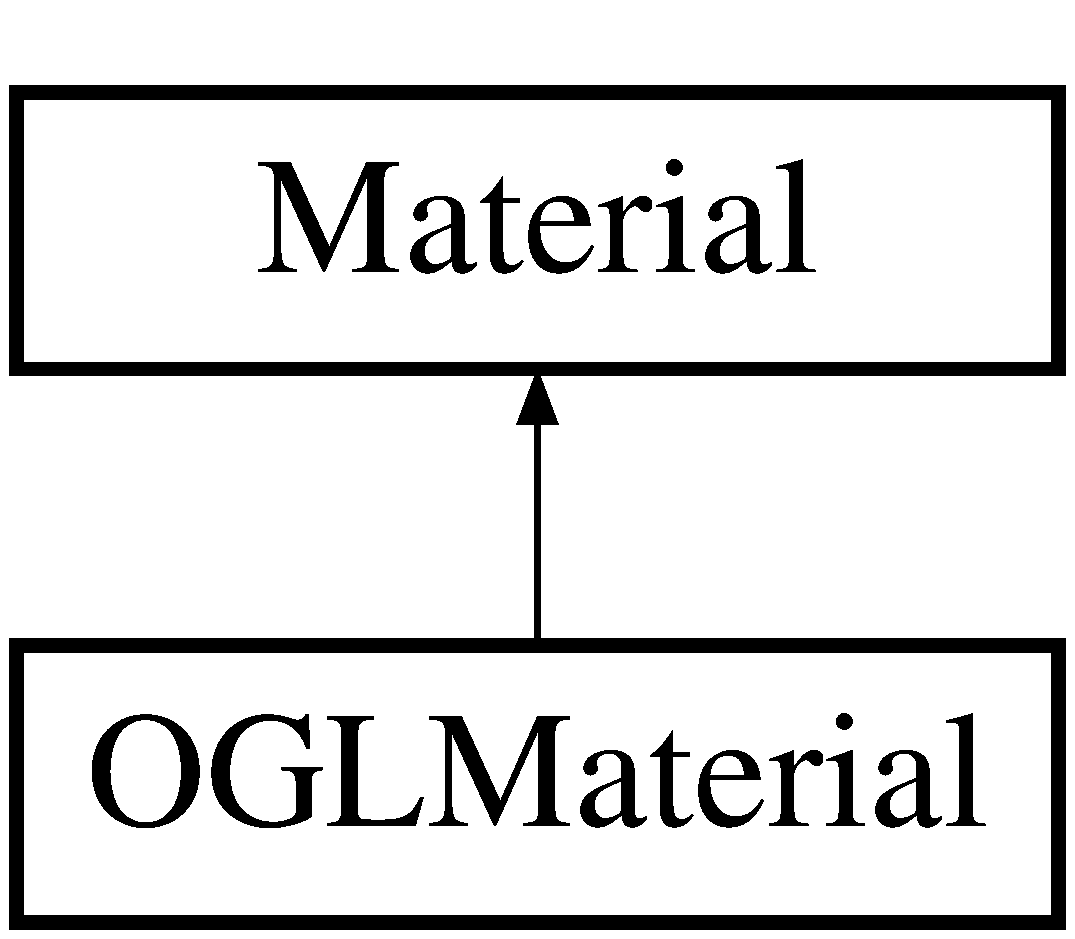
\includegraphics[height=2.000000cm]{class_o_g_l_material}
\end{center}
\end{figure}
\subsection*{Public Types}
\begin{DoxyCompactItemize}
\item 
enum \hyperlink{class_o_g_l_material_a1fc530fc808e270be78c8b296abed0ce}{Material\+Float3\+Property\+Id} \{ \\*
\hyperlink{class_o_g_l_material_a1fc530fc808e270be78c8b296abed0cea5441c93ee26296cf73099ab3ece3bae8}{Ambient}, 
\hyperlink{class_o_g_l_material_a1fc530fc808e270be78c8b296abed0ceabcd3b10f0373f4b2c8d4c5cfa099a04d}{Diffuse}, 
\hyperlink{class_o_g_l_material_a1fc530fc808e270be78c8b296abed0cea59f42bc1358ab6a7640040c4d2ea2513}{Specular}, 
\hyperlink{class_o_g_l_material_a1fc530fc808e270be78c8b296abed0cea6f7a7d603da029b7fe179988a8d19a20}{Emissive}, 
\\*
\hyperlink{class_o_g_l_material_a1fc530fc808e270be78c8b296abed0cea909fa47c1a6d8791f545c2121ecc671a}{Transparent}, 
\hyperlink{class_o_g_l_material_a1fc530fc808e270be78c8b296abed0cead1b4915dec43de7b45c30e32cf80b254}{M\+A\+T\+E\+R\+I\+A\+L\+\_\+\+F\+L\+O\+A\+T3\+\_\+\+P\+R\+O\+P\+E\+R\+T\+Y\+\_\+\+I\+D\+\_\+\+M\+A\+X}
 \}
\item 
enum \hyperlink{class_o_g_l_material_a27506550fa395365703eb941e525e64c}{Material\+Float1\+Property\+Id} \{ \\*
\hyperlink{class_o_g_l_material_a27506550fa395365703eb941e525e64ca149b3ad56ea941570eaa8d0e410f40a3}{Opacity}, 
\hyperlink{class_o_g_l_material_a27506550fa395365703eb941e525e64ca050b45ca29d9c2a74e8ffbb1578695d7}{Shininess}, 
\hyperlink{class_o_g_l_material_a27506550fa395365703eb941e525e64cae4da774c172596772d727db4b5e2cbc0}{Shininess\+Strenght}, 
\hyperlink{class_o_g_l_material_a27506550fa395365703eb941e525e64ca04b1f363f2e457e090414c96c7047536}{Refraction\+Index}, 
\\*
\hyperlink{class_o_g_l_material_a27506550fa395365703eb941e525e64ca681b13f840ad6eec84c56785b91ae292}{M\+A\+T\+E\+R\+I\+A\+L\+\_\+\+F\+L\+O\+A\+T1\+\_\+\+P\+R\+O\+P\+E\+R\+T\+Y\+\_\+\+I\+D\+\_\+\+M\+A\+X}
 \}
\item 
enum \hyperlink{class_o_g_l_material_a79448ba294d1923d56ebca495b0c272e}{Material\+U\+Int1\+Property\+Id} \{ \hyperlink{class_o_g_l_material_a79448ba294d1923d56ebca495b0c272ea410bf1c2f3618546e7327e5dfb8fcf49}{Normal\+Mapping}, 
\hyperlink{class_o_g_l_material_a79448ba294d1923d56ebca495b0c272eaf59f117beb217c8aaa7d149343cde78a}{M\+A\+T\+E\+R\+I\+A\+L\+\_\+\+U\+I\+N\+T1\+\_\+\+P\+R\+O\+P\+E\+R\+T\+Y\+\_\+\+I\+D\+\_\+\+M\+A\+X}
 \}
\item 
enum \hyperlink{class_o_g_l_material_a00ec5436848c78403b6663c2a02f088f}{Shading\+Mode} \{ \\*
\hyperlink{class_o_g_l_material_a00ec5436848c78403b6663c2a02f088fa42b56337fd1dc43656d50d2fde662a23}{Flat}, 
\hyperlink{class_o_g_l_material_a00ec5436848c78403b6663c2a02f088fa0325ae38b5ee6bd8ae52bac388349bee}{Gourad}, 
\hyperlink{class_o_g_l_material_a00ec5436848c78403b6663c2a02f088fac225445a53951d9137587f735657f543}{Phong}, 
\hyperlink{class_o_g_l_material_a00ec5436848c78403b6663c2a02f088fae5a55ff69e3fc8bdb83f921cdd3a9a3c}{Blinn}, 
\\*
\hyperlink{class_o_g_l_material_a00ec5436848c78403b6663c2a02f088fa3f5f6ecc390dbfbec5b68643661fe076}{Toon}, 
\hyperlink{class_o_g_l_material_a00ec5436848c78403b6663c2a02f088faa2ca11b89f8a245872e4b05ae4031d13}{Oren\+Nayar}, 
\hyperlink{class_o_g_l_material_a00ec5436848c78403b6663c2a02f088fac432798ece11cf67f7bd7db9fdfbf730}{Minnaert}, 
\hyperlink{class_o_g_l_material_a00ec5436848c78403b6663c2a02f088fad9a50343accc4627efef4f59d7cf6444}{Cook\+Torrance}, 
\\*
\hyperlink{class_o_g_l_material_a00ec5436848c78403b6663c2a02f088faa350570138ca7bb576e6badcdc23616e}{No\+Shading}, 
\hyperlink{class_o_g_l_material_a00ec5436848c78403b6663c2a02f088fa210b041c2fcfecb49a4fdd1095296eac}{Fresnel}
 \}
\item 
enum \hyperlink{class_o_g_l_material_acd49212071e5ca8ff7093a7536186271}{Blend\+Mode} \{ \hyperlink{class_o_g_l_material_acd49212071e5ca8ff7093a7536186271ad8fb02dd08e3a1b9030886bec1aef727}{Default}, 
\hyperlink{class_o_g_l_material_acd49212071e5ca8ff7093a7536186271a003e5426d86969aefced5427cd2dd540}{Additive}
 \}
\end{DoxyCompactItemize}
\subsection*{Public Member Functions}
\begin{DoxyCompactItemize}
\item 
bool \hyperlink{class_o_g_l_material_a877ee9c7b6125f4a11508a3ea47581b0}{Has\+Texture} (\hyperlink{class_raw_texture_ac0eafe7206f7f38aeb4e8e5631480f6d}{Raw\+Texture\+::\+Texture\+Type} tex\+Type) const 
\item 
void \hyperlink{class_o_g_l_material_a4d4de708b2dc2db1693e7d451d0d4941}{Add\+Texture} (const std\+::shared\+\_\+ptr$<$ \hyperlink{class_o_g_l_texture2_d}{O\+G\+L\+Texture2\+D} $>$ \&sp\+Texture, \hyperlink{class_raw_texture_ac0eafe7206f7f38aeb4e8e5631480f6d}{Raw\+Texture\+::\+Texture\+Type} tex\+Type)
\item 
void \hyperlink{class_o_g_l_material_a0b125e4861e997f7502944fe46382afd}{Set\+Material\+Uniforms} ()
\item 
\hyperlink{class_o_g_l_material_a57900a77e7dd93a1285816d4aa437248}{O\+G\+L\+Material} ()
\item 
virtual \hyperlink{class_o_g_l_material_ac27d566580885dedcb6b4c3dca50693b}{$\sim$\+O\+G\+L\+Material} ()
\end{DoxyCompactItemize}
\subsection*{Public Attributes}
\begin{DoxyCompactItemize}
\item 
std\+::string \hyperlink{class_o_g_l_material_ad8c2aa701fa7d127dec2c3c4a4349ba4}{name}
\end{DoxyCompactItemize}
\subsection*{Static Public Attributes}
\begin{DoxyCompactItemize}
\item 
static glm\+::vec3 \hyperlink{class_o_g_l_material_a7a222f0ece12097de05a1494144c3e27}{White} = glm\+::vec3(1.\+0f)
\item 
static glm\+::vec3 \hyperlink{class_o_g_l_material_acaeb2445a5f20d990e0667a8cdcec863}{Black} = glm\+::vec3(1.\+0f)
\end{DoxyCompactItemize}


\subsection{Detailed Description}


Definition at line 21 of file material.\+h.



\subsection{Member Enumeration Documentation}
\hypertarget{class_o_g_l_material_acd49212071e5ca8ff7093a7536186271}{}\index{O\+G\+L\+Material@{O\+G\+L\+Material}!Blend\+Mode@{Blend\+Mode}}
\index{Blend\+Mode@{Blend\+Mode}!O\+G\+L\+Material@{O\+G\+L\+Material}}
\subsubsection[{Blend\+Mode}]{\setlength{\rightskip}{0pt plus 5cm}enum {\bf O\+G\+L\+Material\+::\+Blend\+Mode}}\label{class_o_g_l_material_acd49212071e5ca8ff7093a7536186271}
\begin{Desc}
\item[Enumerator]\par
\begin{description}
\index{Default@{Default}!O\+G\+L\+Material@{O\+G\+L\+Material}}\index{O\+G\+L\+Material@{O\+G\+L\+Material}!Default@{Default}}\item[{\em 
\hypertarget{class_o_g_l_material_acd49212071e5ca8ff7093a7536186271ad8fb02dd08e3a1b9030886bec1aef727}{}Default\label{class_o_g_l_material_acd49212071e5ca8ff7093a7536186271ad8fb02dd08e3a1b9030886bec1aef727}
}]\index{Additive@{Additive}!O\+G\+L\+Material@{O\+G\+L\+Material}}\index{O\+G\+L\+Material@{O\+G\+L\+Material}!Additive@{Additive}}\item[{\em 
\hypertarget{class_o_g_l_material_acd49212071e5ca8ff7093a7536186271a003e5426d86969aefced5427cd2dd540}{}Additive\label{class_o_g_l_material_acd49212071e5ca8ff7093a7536186271a003e5426d86969aefced5427cd2dd540}
}]\end{description}
\end{Desc}


Definition at line 63 of file material.\+h.

\hypertarget{class_o_g_l_material_a27506550fa395365703eb941e525e64c}{}\index{O\+G\+L\+Material@{O\+G\+L\+Material}!Material\+Float1\+Property\+Id@{Material\+Float1\+Property\+Id}}
\index{Material\+Float1\+Property\+Id@{Material\+Float1\+Property\+Id}!O\+G\+L\+Material@{O\+G\+L\+Material}}
\subsubsection[{Material\+Float1\+Property\+Id}]{\setlength{\rightskip}{0pt plus 5cm}enum {\bf O\+G\+L\+Material\+::\+Material\+Float1\+Property\+Id}}\label{class_o_g_l_material_a27506550fa395365703eb941e525e64c}
\begin{Desc}
\item[Enumerator]\par
\begin{description}
\index{Opacity@{Opacity}!O\+G\+L\+Material@{O\+G\+L\+Material}}\index{O\+G\+L\+Material@{O\+G\+L\+Material}!Opacity@{Opacity}}\item[{\em 
\hypertarget{class_o_g_l_material_a27506550fa395365703eb941e525e64ca149b3ad56ea941570eaa8d0e410f40a3}{}Opacity\label{class_o_g_l_material_a27506550fa395365703eb941e525e64ca149b3ad56ea941570eaa8d0e410f40a3}
}]\index{Shininess@{Shininess}!O\+G\+L\+Material@{O\+G\+L\+Material}}\index{O\+G\+L\+Material@{O\+G\+L\+Material}!Shininess@{Shininess}}\item[{\em 
\hypertarget{class_o_g_l_material_a27506550fa395365703eb941e525e64ca050b45ca29d9c2a74e8ffbb1578695d7}{}Shininess\label{class_o_g_l_material_a27506550fa395365703eb941e525e64ca050b45ca29d9c2a74e8ffbb1578695d7}
}]\index{Shininess\+Strenght@{Shininess\+Strenght}!O\+G\+L\+Material@{O\+G\+L\+Material}}\index{O\+G\+L\+Material@{O\+G\+L\+Material}!Shininess\+Strenght@{Shininess\+Strenght}}\item[{\em 
\hypertarget{class_o_g_l_material_a27506550fa395365703eb941e525e64cae4da774c172596772d727db4b5e2cbc0}{}Shininess\+Strenght\label{class_o_g_l_material_a27506550fa395365703eb941e525e64cae4da774c172596772d727db4b5e2cbc0}
}]\index{Refraction\+Index@{Refraction\+Index}!O\+G\+L\+Material@{O\+G\+L\+Material}}\index{O\+G\+L\+Material@{O\+G\+L\+Material}!Refraction\+Index@{Refraction\+Index}}\item[{\em 
\hypertarget{class_o_g_l_material_a27506550fa395365703eb941e525e64ca04b1f363f2e457e090414c96c7047536}{}Refraction\+Index\label{class_o_g_l_material_a27506550fa395365703eb941e525e64ca04b1f363f2e457e090414c96c7047536}
}]\index{M\+A\+T\+E\+R\+I\+A\+L\+\_\+\+F\+L\+O\+A\+T1\+\_\+\+P\+R\+O\+P\+E\+R\+T\+Y\+\_\+\+I\+D\+\_\+\+M\+A\+X@{M\+A\+T\+E\+R\+I\+A\+L\+\_\+\+F\+L\+O\+A\+T1\+\_\+\+P\+R\+O\+P\+E\+R\+T\+Y\+\_\+\+I\+D\+\_\+\+M\+A\+X}!O\+G\+L\+Material@{O\+G\+L\+Material}}\index{O\+G\+L\+Material@{O\+G\+L\+Material}!M\+A\+T\+E\+R\+I\+A\+L\+\_\+\+F\+L\+O\+A\+T1\+\_\+\+P\+R\+O\+P\+E\+R\+T\+Y\+\_\+\+I\+D\+\_\+\+M\+A\+X@{M\+A\+T\+E\+R\+I\+A\+L\+\_\+\+F\+L\+O\+A\+T1\+\_\+\+P\+R\+O\+P\+E\+R\+T\+Y\+\_\+\+I\+D\+\_\+\+M\+A\+X}}\item[{\em 
\hypertarget{class_o_g_l_material_a27506550fa395365703eb941e525e64ca681b13f840ad6eec84c56785b91ae292}{}M\+A\+T\+E\+R\+I\+A\+L\+\_\+\+F\+L\+O\+A\+T1\+\_\+\+P\+R\+O\+P\+E\+R\+T\+Y\+\_\+\+I\+D\+\_\+\+M\+A\+X\label{class_o_g_l_material_a27506550fa395365703eb941e525e64ca681b13f840ad6eec84c56785b91ae292}
}]\end{description}
\end{Desc}


Definition at line 36 of file material.\+h.

\hypertarget{class_o_g_l_material_a1fc530fc808e270be78c8b296abed0ce}{}\index{O\+G\+L\+Material@{O\+G\+L\+Material}!Material\+Float3\+Property\+Id@{Material\+Float3\+Property\+Id}}
\index{Material\+Float3\+Property\+Id@{Material\+Float3\+Property\+Id}!O\+G\+L\+Material@{O\+G\+L\+Material}}
\subsubsection[{Material\+Float3\+Property\+Id}]{\setlength{\rightskip}{0pt plus 5cm}enum {\bf O\+G\+L\+Material\+::\+Material\+Float3\+Property\+Id}}\label{class_o_g_l_material_a1fc530fc808e270be78c8b296abed0ce}
\begin{Desc}
\item[Enumerator]\par
\begin{description}
\index{Ambient@{Ambient}!O\+G\+L\+Material@{O\+G\+L\+Material}}\index{O\+G\+L\+Material@{O\+G\+L\+Material}!Ambient@{Ambient}}\item[{\em 
\hypertarget{class_o_g_l_material_a1fc530fc808e270be78c8b296abed0cea5441c93ee26296cf73099ab3ece3bae8}{}Ambient\label{class_o_g_l_material_a1fc530fc808e270be78c8b296abed0cea5441c93ee26296cf73099ab3ece3bae8}
}]\index{Diffuse@{Diffuse}!O\+G\+L\+Material@{O\+G\+L\+Material}}\index{O\+G\+L\+Material@{O\+G\+L\+Material}!Diffuse@{Diffuse}}\item[{\em 
\hypertarget{class_o_g_l_material_a1fc530fc808e270be78c8b296abed0ceabcd3b10f0373f4b2c8d4c5cfa099a04d}{}Diffuse\label{class_o_g_l_material_a1fc530fc808e270be78c8b296abed0ceabcd3b10f0373f4b2c8d4c5cfa099a04d}
}]\index{Specular@{Specular}!O\+G\+L\+Material@{O\+G\+L\+Material}}\index{O\+G\+L\+Material@{O\+G\+L\+Material}!Specular@{Specular}}\item[{\em 
\hypertarget{class_o_g_l_material_a1fc530fc808e270be78c8b296abed0cea59f42bc1358ab6a7640040c4d2ea2513}{}Specular\label{class_o_g_l_material_a1fc530fc808e270be78c8b296abed0cea59f42bc1358ab6a7640040c4d2ea2513}
}]\index{Emissive@{Emissive}!O\+G\+L\+Material@{O\+G\+L\+Material}}\index{O\+G\+L\+Material@{O\+G\+L\+Material}!Emissive@{Emissive}}\item[{\em 
\hypertarget{class_o_g_l_material_a1fc530fc808e270be78c8b296abed0cea6f7a7d603da029b7fe179988a8d19a20}{}Emissive\label{class_o_g_l_material_a1fc530fc808e270be78c8b296abed0cea6f7a7d603da029b7fe179988a8d19a20}
}]\index{Transparent@{Transparent}!O\+G\+L\+Material@{O\+G\+L\+Material}}\index{O\+G\+L\+Material@{O\+G\+L\+Material}!Transparent@{Transparent}}\item[{\em 
\hypertarget{class_o_g_l_material_a1fc530fc808e270be78c8b296abed0cea909fa47c1a6d8791f545c2121ecc671a}{}Transparent\label{class_o_g_l_material_a1fc530fc808e270be78c8b296abed0cea909fa47c1a6d8791f545c2121ecc671a}
}]\index{M\+A\+T\+E\+R\+I\+A\+L\+\_\+\+F\+L\+O\+A\+T3\+\_\+\+P\+R\+O\+P\+E\+R\+T\+Y\+\_\+\+I\+D\+\_\+\+M\+A\+X@{M\+A\+T\+E\+R\+I\+A\+L\+\_\+\+F\+L\+O\+A\+T3\+\_\+\+P\+R\+O\+P\+E\+R\+T\+Y\+\_\+\+I\+D\+\_\+\+M\+A\+X}!O\+G\+L\+Material@{O\+G\+L\+Material}}\index{O\+G\+L\+Material@{O\+G\+L\+Material}!M\+A\+T\+E\+R\+I\+A\+L\+\_\+\+F\+L\+O\+A\+T3\+\_\+\+P\+R\+O\+P\+E\+R\+T\+Y\+\_\+\+I\+D\+\_\+\+M\+A\+X@{M\+A\+T\+E\+R\+I\+A\+L\+\_\+\+F\+L\+O\+A\+T3\+\_\+\+P\+R\+O\+P\+E\+R\+T\+Y\+\_\+\+I\+D\+\_\+\+M\+A\+X}}\item[{\em 
\hypertarget{class_o_g_l_material_a1fc530fc808e270be78c8b296abed0cead1b4915dec43de7b45c30e32cf80b254}{}M\+A\+T\+E\+R\+I\+A\+L\+\_\+\+F\+L\+O\+A\+T3\+\_\+\+P\+R\+O\+P\+E\+R\+T\+Y\+\_\+\+I\+D\+\_\+\+M\+A\+X\label{class_o_g_l_material_a1fc530fc808e270be78c8b296abed0cead1b4915dec43de7b45c30e32cf80b254}
}]\end{description}
\end{Desc}


Definition at line 27 of file material.\+h.

\hypertarget{class_o_g_l_material_a79448ba294d1923d56ebca495b0c272e}{}\index{O\+G\+L\+Material@{O\+G\+L\+Material}!Material\+U\+Int1\+Property\+Id@{Material\+U\+Int1\+Property\+Id}}
\index{Material\+U\+Int1\+Property\+Id@{Material\+U\+Int1\+Property\+Id}!O\+G\+L\+Material@{O\+G\+L\+Material}}
\subsubsection[{Material\+U\+Int1\+Property\+Id}]{\setlength{\rightskip}{0pt plus 5cm}enum {\bf O\+G\+L\+Material\+::\+Material\+U\+Int1\+Property\+Id}}\label{class_o_g_l_material_a79448ba294d1923d56ebca495b0c272e}
\begin{Desc}
\item[Enumerator]\par
\begin{description}
\index{Normal\+Mapping@{Normal\+Mapping}!O\+G\+L\+Material@{O\+G\+L\+Material}}\index{O\+G\+L\+Material@{O\+G\+L\+Material}!Normal\+Mapping@{Normal\+Mapping}}\item[{\em 
\hypertarget{class_o_g_l_material_a79448ba294d1923d56ebca495b0c272ea410bf1c2f3618546e7327e5dfb8fcf49}{}Normal\+Mapping\label{class_o_g_l_material_a79448ba294d1923d56ebca495b0c272ea410bf1c2f3618546e7327e5dfb8fcf49}
}]\index{M\+A\+T\+E\+R\+I\+A\+L\+\_\+\+U\+I\+N\+T1\+\_\+\+P\+R\+O\+P\+E\+R\+T\+Y\+\_\+\+I\+D\+\_\+\+M\+A\+X@{M\+A\+T\+E\+R\+I\+A\+L\+\_\+\+U\+I\+N\+T1\+\_\+\+P\+R\+O\+P\+E\+R\+T\+Y\+\_\+\+I\+D\+\_\+\+M\+A\+X}!O\+G\+L\+Material@{O\+G\+L\+Material}}\index{O\+G\+L\+Material@{O\+G\+L\+Material}!M\+A\+T\+E\+R\+I\+A\+L\+\_\+\+U\+I\+N\+T1\+\_\+\+P\+R\+O\+P\+E\+R\+T\+Y\+\_\+\+I\+D\+\_\+\+M\+A\+X@{M\+A\+T\+E\+R\+I\+A\+L\+\_\+\+U\+I\+N\+T1\+\_\+\+P\+R\+O\+P\+E\+R\+T\+Y\+\_\+\+I\+D\+\_\+\+M\+A\+X}}\item[{\em 
\hypertarget{class_o_g_l_material_a79448ba294d1923d56ebca495b0c272eaf59f117beb217c8aaa7d149343cde78a}{}M\+A\+T\+E\+R\+I\+A\+L\+\_\+\+U\+I\+N\+T1\+\_\+\+P\+R\+O\+P\+E\+R\+T\+Y\+\_\+\+I\+D\+\_\+\+M\+A\+X\label{class_o_g_l_material_a79448ba294d1923d56ebca495b0c272eaf59f117beb217c8aaa7d149343cde78a}
}]\end{description}
\end{Desc}


Definition at line 44 of file material.\+h.

\hypertarget{class_o_g_l_material_a00ec5436848c78403b6663c2a02f088f}{}\index{O\+G\+L\+Material@{O\+G\+L\+Material}!Shading\+Mode@{Shading\+Mode}}
\index{Shading\+Mode@{Shading\+Mode}!O\+G\+L\+Material@{O\+G\+L\+Material}}
\subsubsection[{Shading\+Mode}]{\setlength{\rightskip}{0pt plus 5cm}enum {\bf O\+G\+L\+Material\+::\+Shading\+Mode}}\label{class_o_g_l_material_a00ec5436848c78403b6663c2a02f088f}
\begin{Desc}
\item[Enumerator]\par
\begin{description}
\index{Flat@{Flat}!O\+G\+L\+Material@{O\+G\+L\+Material}}\index{O\+G\+L\+Material@{O\+G\+L\+Material}!Flat@{Flat}}\item[{\em 
\hypertarget{class_o_g_l_material_a00ec5436848c78403b6663c2a02f088fa42b56337fd1dc43656d50d2fde662a23}{}Flat\label{class_o_g_l_material_a00ec5436848c78403b6663c2a02f088fa42b56337fd1dc43656d50d2fde662a23}
}]\index{Gourad@{Gourad}!O\+G\+L\+Material@{O\+G\+L\+Material}}\index{O\+G\+L\+Material@{O\+G\+L\+Material}!Gourad@{Gourad}}\item[{\em 
\hypertarget{class_o_g_l_material_a00ec5436848c78403b6663c2a02f088fa0325ae38b5ee6bd8ae52bac388349bee}{}Gourad\label{class_o_g_l_material_a00ec5436848c78403b6663c2a02f088fa0325ae38b5ee6bd8ae52bac388349bee}
}]\index{Phong@{Phong}!O\+G\+L\+Material@{O\+G\+L\+Material}}\index{O\+G\+L\+Material@{O\+G\+L\+Material}!Phong@{Phong}}\item[{\em 
\hypertarget{class_o_g_l_material_a00ec5436848c78403b6663c2a02f088fac225445a53951d9137587f735657f543}{}Phong\label{class_o_g_l_material_a00ec5436848c78403b6663c2a02f088fac225445a53951d9137587f735657f543}
}]\index{Blinn@{Blinn}!O\+G\+L\+Material@{O\+G\+L\+Material}}\index{O\+G\+L\+Material@{O\+G\+L\+Material}!Blinn@{Blinn}}\item[{\em 
\hypertarget{class_o_g_l_material_a00ec5436848c78403b6663c2a02f088fae5a55ff69e3fc8bdb83f921cdd3a9a3c}{}Blinn\label{class_o_g_l_material_a00ec5436848c78403b6663c2a02f088fae5a55ff69e3fc8bdb83f921cdd3a9a3c}
}]\index{Toon@{Toon}!O\+G\+L\+Material@{O\+G\+L\+Material}}\index{O\+G\+L\+Material@{O\+G\+L\+Material}!Toon@{Toon}}\item[{\em 
\hypertarget{class_o_g_l_material_a00ec5436848c78403b6663c2a02f088fa3f5f6ecc390dbfbec5b68643661fe076}{}Toon\label{class_o_g_l_material_a00ec5436848c78403b6663c2a02f088fa3f5f6ecc390dbfbec5b68643661fe076}
}]\index{Oren\+Nayar@{Oren\+Nayar}!O\+G\+L\+Material@{O\+G\+L\+Material}}\index{O\+G\+L\+Material@{O\+G\+L\+Material}!Oren\+Nayar@{Oren\+Nayar}}\item[{\em 
\hypertarget{class_o_g_l_material_a00ec5436848c78403b6663c2a02f088faa2ca11b89f8a245872e4b05ae4031d13}{}Oren\+Nayar\label{class_o_g_l_material_a00ec5436848c78403b6663c2a02f088faa2ca11b89f8a245872e4b05ae4031d13}
}]\index{Minnaert@{Minnaert}!O\+G\+L\+Material@{O\+G\+L\+Material}}\index{O\+G\+L\+Material@{O\+G\+L\+Material}!Minnaert@{Minnaert}}\item[{\em 
\hypertarget{class_o_g_l_material_a00ec5436848c78403b6663c2a02f088fac432798ece11cf67f7bd7db9fdfbf730}{}Minnaert\label{class_o_g_l_material_a00ec5436848c78403b6663c2a02f088fac432798ece11cf67f7bd7db9fdfbf730}
}]\index{Cook\+Torrance@{Cook\+Torrance}!O\+G\+L\+Material@{O\+G\+L\+Material}}\index{O\+G\+L\+Material@{O\+G\+L\+Material}!Cook\+Torrance@{Cook\+Torrance}}\item[{\em 
\hypertarget{class_o_g_l_material_a00ec5436848c78403b6663c2a02f088fad9a50343accc4627efef4f59d7cf6444}{}Cook\+Torrance\label{class_o_g_l_material_a00ec5436848c78403b6663c2a02f088fad9a50343accc4627efef4f59d7cf6444}
}]\index{No\+Shading@{No\+Shading}!O\+G\+L\+Material@{O\+G\+L\+Material}}\index{O\+G\+L\+Material@{O\+G\+L\+Material}!No\+Shading@{No\+Shading}}\item[{\em 
\hypertarget{class_o_g_l_material_a00ec5436848c78403b6663c2a02f088faa350570138ca7bb576e6badcdc23616e}{}No\+Shading\label{class_o_g_l_material_a00ec5436848c78403b6663c2a02f088faa350570138ca7bb576e6badcdc23616e}
}]\index{Fresnel@{Fresnel}!O\+G\+L\+Material@{O\+G\+L\+Material}}\index{O\+G\+L\+Material@{O\+G\+L\+Material}!Fresnel@{Fresnel}}\item[{\em 
\hypertarget{class_o_g_l_material_a00ec5436848c78403b6663c2a02f088fa210b041c2fcfecb49a4fdd1095296eac}{}Fresnel\label{class_o_g_l_material_a00ec5436848c78403b6663c2a02f088fa210b041c2fcfecb49a4fdd1095296eac}
}]\end{description}
\end{Desc}


Definition at line 50 of file material.\+h.



\subsection{Constructor \& Destructor Documentation}
\hypertarget{class_o_g_l_material_a57900a77e7dd93a1285816d4aa437248}{}\index{O\+G\+L\+Material@{O\+G\+L\+Material}!O\+G\+L\+Material@{O\+G\+L\+Material}}
\index{O\+G\+L\+Material@{O\+G\+L\+Material}!O\+G\+L\+Material@{O\+G\+L\+Material}}
\subsubsection[{O\+G\+L\+Material()}]{\setlength{\rightskip}{0pt plus 5cm}O\+G\+L\+Material\+::\+O\+G\+L\+Material (
\begin{DoxyParamCaption}
{}
\end{DoxyParamCaption}
)}\label{class_o_g_l_material_a57900a77e7dd93a1285816d4aa437248}


Definition at line 48 of file material.\+cpp.

\hypertarget{class_o_g_l_material_ac27d566580885dedcb6b4c3dca50693b}{}\index{O\+G\+L\+Material@{O\+G\+L\+Material}!````~O\+G\+L\+Material@{$\sim$\+O\+G\+L\+Material}}
\index{````~O\+G\+L\+Material@{$\sim$\+O\+G\+L\+Material}!O\+G\+L\+Material@{O\+G\+L\+Material}}
\subsubsection[{$\sim$\+O\+G\+L\+Material()}]{\setlength{\rightskip}{0pt plus 5cm}O\+G\+L\+Material\+::$\sim$\+O\+G\+L\+Material (
\begin{DoxyParamCaption}
{}
\end{DoxyParamCaption}
)\hspace{0.3cm}{\ttfamily [virtual]}}\label{class_o_g_l_material_ac27d566580885dedcb6b4c3dca50693b}


Definition at line 54 of file material.\+cpp.



\subsection{Member Function Documentation}
\hypertarget{class_o_g_l_material_a4d4de708b2dc2db1693e7d451d0d4941}{}\index{O\+G\+L\+Material@{O\+G\+L\+Material}!Add\+Texture@{Add\+Texture}}
\index{Add\+Texture@{Add\+Texture}!O\+G\+L\+Material@{O\+G\+L\+Material}}
\subsubsection[{Add\+Texture(const std\+::shared\+\_\+ptr$<$ O\+G\+L\+Texture2\+D $>$ \&sp\+Texture, Raw\+Texture\+::\+Texture\+Type tex\+Type)}]{\setlength{\rightskip}{0pt plus 5cm}void O\+G\+L\+Material\+::\+Add\+Texture (
\begin{DoxyParamCaption}
\item[{const std\+::shared\+\_\+ptr$<$ {\bf O\+G\+L\+Texture2\+D} $>$ \&}]{sp\+Texture, }
\item[{{\bf Raw\+Texture\+::\+Texture\+Type}}]{tex\+Type}
\end{DoxyParamCaption}
)}\label{class_o_g_l_material_a4d4de708b2dc2db1693e7d451d0d4941}


Definition at line 15 of file material.\+cpp.

\hypertarget{class_o_g_l_material_a877ee9c7b6125f4a11508a3ea47581b0}{}\index{O\+G\+L\+Material@{O\+G\+L\+Material}!Has\+Texture@{Has\+Texture}}
\index{Has\+Texture@{Has\+Texture}!O\+G\+L\+Material@{O\+G\+L\+Material}}
\subsubsection[{Has\+Texture(\+Raw\+Texture\+::\+Texture\+Type tex\+Type) const }]{\setlength{\rightskip}{0pt plus 5cm}bool O\+G\+L\+Material\+::\+Has\+Texture (
\begin{DoxyParamCaption}
\item[{{\bf Raw\+Texture\+::\+Texture\+Type}}]{tex\+Type}
\end{DoxyParamCaption}
) const}\label{class_o_g_l_material_a877ee9c7b6125f4a11508a3ea47581b0}


Definition at line 10 of file material.\+cpp.

\hypertarget{class_o_g_l_material_a0b125e4861e997f7502944fe46382afd}{}\index{O\+G\+L\+Material@{O\+G\+L\+Material}!Set\+Material\+Uniforms@{Set\+Material\+Uniforms}}
\index{Set\+Material\+Uniforms@{Set\+Material\+Uniforms}!O\+G\+L\+Material@{O\+G\+L\+Material}}
\subsubsection[{Set\+Material\+Uniforms()}]{\setlength{\rightskip}{0pt plus 5cm}void O\+G\+L\+Material\+::\+Set\+Material\+Uniforms (
\begin{DoxyParamCaption}
{}
\end{DoxyParamCaption}
)}\label{class_o_g_l_material_a0b125e4861e997f7502944fe46382afd}


Definition at line 21 of file material.\+cpp.



\subsection{Member Data Documentation}
\hypertarget{class_o_g_l_material_acaeb2445a5f20d990e0667a8cdcec863}{}\index{O\+G\+L\+Material@{O\+G\+L\+Material}!Black@{Black}}
\index{Black@{Black}!O\+G\+L\+Material@{O\+G\+L\+Material}}
\subsubsection[{Black}]{\setlength{\rightskip}{0pt plus 5cm}glm\+::vec3 O\+G\+L\+Material\+::\+Black = glm\+::vec3(1.\+0f)\hspace{0.3cm}{\ttfamily [static]}}\label{class_o_g_l_material_acaeb2445a5f20d990e0667a8cdcec863}


Definition at line 69 of file material.\+h.

\hypertarget{class_o_g_l_material_ad8c2aa701fa7d127dec2c3c4a4349ba4}{}\index{O\+G\+L\+Material@{O\+G\+L\+Material}!name@{name}}
\index{name@{name}!O\+G\+L\+Material@{O\+G\+L\+Material}}
\subsubsection[{name}]{\setlength{\rightskip}{0pt plus 5cm}std\+::string O\+G\+L\+Material\+::name}\label{class_o_g_l_material_ad8c2aa701fa7d127dec2c3c4a4349ba4}


Definition at line 71 of file material.\+h.

\hypertarget{class_o_g_l_material_a7a222f0ece12097de05a1494144c3e27}{}\index{O\+G\+L\+Material@{O\+G\+L\+Material}!White@{White}}
\index{White@{White}!O\+G\+L\+Material@{O\+G\+L\+Material}}
\subsubsection[{White}]{\setlength{\rightskip}{0pt plus 5cm}glm\+::vec3 O\+G\+L\+Material\+::\+White = glm\+::vec3(1.\+0f)\hspace{0.3cm}{\ttfamily [static]}}\label{class_o_g_l_material_a7a222f0ece12097de05a1494144c3e27}


Definition at line 68 of file material.\+h.



The documentation for this class was generated from the following files\+:\begin{DoxyCompactItemize}
\item 
V\+C\+T\+\_\+\+Engine/scene/\hyperlink{material_8h}{material.\+h}\item 
V\+C\+T\+\_\+\+Engine/scene/\hyperlink{material_8cpp}{material.\+cpp}\end{DoxyCompactItemize}

\hypertarget{class_o_g_l_mesh}{}\section{O\+G\+L\+Mesh Class Reference}
\label{class_o_g_l_mesh}\index{O\+G\+L\+Mesh@{O\+G\+L\+Mesh}}


{\ttfamily \#include $<$mesh.\+h$>$}

Inheritance diagram for O\+G\+L\+Mesh\+:\begin{figure}[H]
\begin{center}
\leavevmode
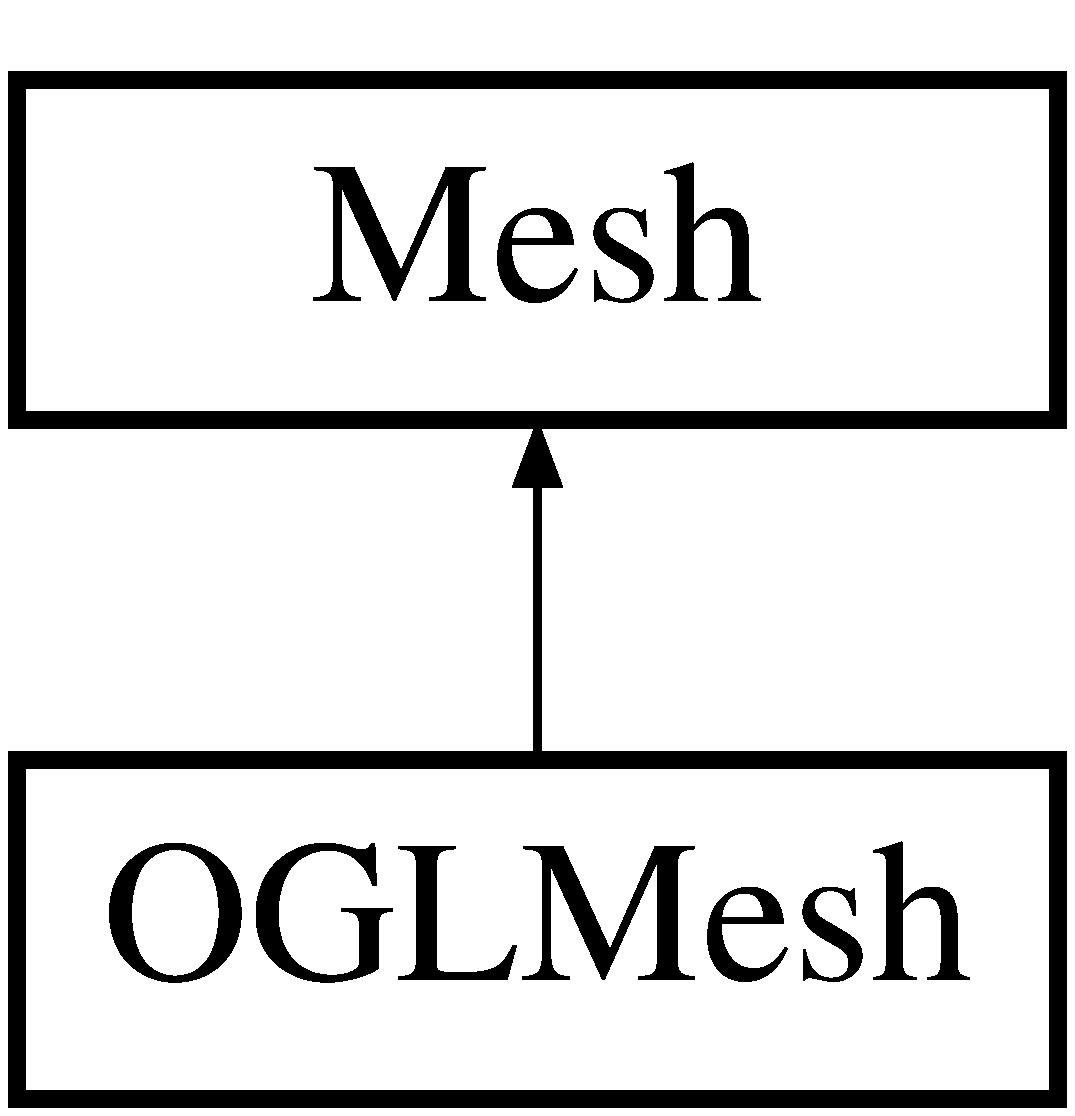
\includegraphics[height=2.000000cm]{class_o_g_l_mesh}
\end{center}
\end{figure}
\subsection*{Public Member Functions}
\begin{DoxyCompactItemize}
\item 
\hyperlink{class_o_g_l_mesh_ab16637bce9f72105cbc661949926d4fd}{O\+G\+L\+Mesh} ()
\item 
virtual \hyperlink{class_o_g_l_mesh_a81d6ba27b650afaf6dd67df8508068c1}{$\sim$\+O\+G\+L\+Mesh} ()
\item 
void \hyperlink{class_o_g_l_mesh_a7d36e3fe07a85a0d50eced4e4ed9105f}{Upload\+To\+G\+P\+U} (bool unload\+From\+R\+A\+M=true)
\item 
void \hyperlink{class_o_g_l_mesh_a1a484d2250debeda7049192f35ce8203}{Bind\+Array\+Buffer} ()
\item 
void \hyperlink{class_o_g_l_mesh_ac8be151a624619d6710717b34b2a974d}{Bind\+Element\+Array\+Buffer} ()
\item 
void \hyperlink{class_o_g_l_mesh_a1142d41844f6c3a094ef6c7a1be95df7}{Bind\+Vertex\+Array\+Object} ()
\item 
void \hyperlink{class_o_g_l_mesh_a3811dabaecf72be0c5c106bf9fccc020}{Buffer\+Pointers} (oglplus\+::\+Program \&program)
\item 
void \hyperlink{class_o_g_l_mesh_a88a57d48eabc18f11d2ec6938075ec41}{Buffer\+Setup} (oglplus\+::\+Program \&program)
\item 
void \hyperlink{class_o_g_l_mesh_a5b4182b63fe4f4cbd11d525526eefbb2}{Draw\+Elements} ()
\item 
bool \hyperlink{class_o_g_l_mesh_ac83aaa629d5033acbe69f9a98703d6cf}{On\+G\+P\+U\+Memory} () const 
\end{DoxyCompactItemize}
\subsection*{Protected Attributes}
\begin{DoxyCompactItemize}
\item 
std\+::unique\+\_\+ptr$<$ oglplus\+::\+Buffer $>$ \hyperlink{class_o_g_l_mesh_add6dba0a9c25b3861ddb1dae4ce61dc0}{ogl\+Array\+Buffer}
\item 
std\+::unique\+\_\+ptr$<$ oglplus\+::\+Buffer $>$ \hyperlink{class_o_g_l_mesh_aa6ee45949ecaec113ad8062d1b601bec}{ogl\+Element\+Array\+Buffer}
\item 
std\+::unique\+\_\+ptr$<$ oglplus\+::\+Vertex\+Array $>$ \hyperlink{class_o_g_l_mesh_acf47aa123c36d1d06c2d71b13787b0e6}{ogl\+Vertex\+Array}
\item 
bool \hyperlink{class_o_g_l_mesh_aaa6cd7e62890961f6114d9753b7b3b58}{on\+G\+P\+U\+Memory}
\item 
unsigned int \hyperlink{class_o_g_l_mesh_a745e6b366f6323cbf0edd78aa76b868a}{indices\+Count}
\item 
unsigned int \hyperlink{class_o_g_l_mesh_a881b075268f51d438d4242d2380981ab}{vertex\+Count}
\end{DoxyCompactItemize}
\subsection*{Static Protected Attributes}
\begin{DoxyCompactItemize}
\item 
static oglplus\+::\+Context \hyperlink{class_o_g_l_mesh_ab63eb6d70cd8760e8aa2cb6833fe066b}{gl}
\end{DoxyCompactItemize}
\subsection*{Additional Inherited Members}


\subsection{Detailed Description}


Definition at line 26 of file mesh.\+h.



\subsection{Constructor \& Destructor Documentation}
\hypertarget{class_o_g_l_mesh_ab16637bce9f72105cbc661949926d4fd}{}\index{O\+G\+L\+Mesh@{O\+G\+L\+Mesh}!O\+G\+L\+Mesh@{O\+G\+L\+Mesh}}
\index{O\+G\+L\+Mesh@{O\+G\+L\+Mesh}!O\+G\+L\+Mesh@{O\+G\+L\+Mesh}}
\subsubsection[{O\+G\+L\+Mesh()}]{\setlength{\rightskip}{0pt plus 5cm}O\+G\+L\+Mesh\+::\+O\+G\+L\+Mesh (
\begin{DoxyParamCaption}
{}
\end{DoxyParamCaption}
)}\label{class_o_g_l_mesh_ab16637bce9f72105cbc661949926d4fd}


Definition at line 22 of file mesh.\+cpp.

\hypertarget{class_o_g_l_mesh_a81d6ba27b650afaf6dd67df8508068c1}{}\index{O\+G\+L\+Mesh@{O\+G\+L\+Mesh}!````~O\+G\+L\+Mesh@{$\sim$\+O\+G\+L\+Mesh}}
\index{````~O\+G\+L\+Mesh@{$\sim$\+O\+G\+L\+Mesh}!O\+G\+L\+Mesh@{O\+G\+L\+Mesh}}
\subsubsection[{$\sim$\+O\+G\+L\+Mesh()}]{\setlength{\rightskip}{0pt plus 5cm}O\+G\+L\+Mesh\+::$\sim$\+O\+G\+L\+Mesh (
\begin{DoxyParamCaption}
{}
\end{DoxyParamCaption}
)\hspace{0.3cm}{\ttfamily [virtual]}}\label{class_o_g_l_mesh_a81d6ba27b650afaf6dd67df8508068c1}


Definition at line 26 of file mesh.\+cpp.



\subsection{Member Function Documentation}
\hypertarget{class_o_g_l_mesh_a1a484d2250debeda7049192f35ce8203}{}\index{O\+G\+L\+Mesh@{O\+G\+L\+Mesh}!Bind\+Array\+Buffer@{Bind\+Array\+Buffer}}
\index{Bind\+Array\+Buffer@{Bind\+Array\+Buffer}!O\+G\+L\+Mesh@{O\+G\+L\+Mesh}}
\subsubsection[{Bind\+Array\+Buffer()}]{\setlength{\rightskip}{0pt plus 5cm}void O\+G\+L\+Mesh\+::\+Bind\+Array\+Buffer (
\begin{DoxyParamCaption}
{}
\end{DoxyParamCaption}
)}\label{class_o_g_l_mesh_a1a484d2250debeda7049192f35ce8203}


Definition at line 71 of file mesh.\+cpp.

\hypertarget{class_o_g_l_mesh_ac8be151a624619d6710717b34b2a974d}{}\index{O\+G\+L\+Mesh@{O\+G\+L\+Mesh}!Bind\+Element\+Array\+Buffer@{Bind\+Element\+Array\+Buffer}}
\index{Bind\+Element\+Array\+Buffer@{Bind\+Element\+Array\+Buffer}!O\+G\+L\+Mesh@{O\+G\+L\+Mesh}}
\subsubsection[{Bind\+Element\+Array\+Buffer()}]{\setlength{\rightskip}{0pt plus 5cm}void O\+G\+L\+Mesh\+::\+Bind\+Element\+Array\+Buffer (
\begin{DoxyParamCaption}
{}
\end{DoxyParamCaption}
)}\label{class_o_g_l_mesh_ac8be151a624619d6710717b34b2a974d}


Definition at line 76 of file mesh.\+cpp.

\hypertarget{class_o_g_l_mesh_a1142d41844f6c3a094ef6c7a1be95df7}{}\index{O\+G\+L\+Mesh@{O\+G\+L\+Mesh}!Bind\+Vertex\+Array\+Object@{Bind\+Vertex\+Array\+Object}}
\index{Bind\+Vertex\+Array\+Object@{Bind\+Vertex\+Array\+Object}!O\+G\+L\+Mesh@{O\+G\+L\+Mesh}}
\subsubsection[{Bind\+Vertex\+Array\+Object()}]{\setlength{\rightskip}{0pt plus 5cm}void O\+G\+L\+Mesh\+::\+Bind\+Vertex\+Array\+Object (
\begin{DoxyParamCaption}
{}
\end{DoxyParamCaption}
)}\label{class_o_g_l_mesh_a1142d41844f6c3a094ef6c7a1be95df7}


Definition at line 81 of file mesh.\+cpp.

\hypertarget{class_o_g_l_mesh_a3811dabaecf72be0c5c106bf9fccc020}{}\index{O\+G\+L\+Mesh@{O\+G\+L\+Mesh}!Buffer\+Pointers@{Buffer\+Pointers}}
\index{Buffer\+Pointers@{Buffer\+Pointers}!O\+G\+L\+Mesh@{O\+G\+L\+Mesh}}
\subsubsection[{Buffer\+Pointers(oglplus\+::\+Program \&program)}]{\setlength{\rightskip}{0pt plus 5cm}void O\+G\+L\+Mesh\+::\+Buffer\+Pointers (
\begin{DoxyParamCaption}
\item[{oglplus\+::\+Program \&}]{program}
\end{DoxyParamCaption}
)}\label{class_o_g_l_mesh_a3811dabaecf72be0c5c106bf9fccc020}


Definition at line 92 of file mesh.\+cpp.

\hypertarget{class_o_g_l_mesh_a88a57d48eabc18f11d2ec6938075ec41}{}\index{O\+G\+L\+Mesh@{O\+G\+L\+Mesh}!Buffer\+Setup@{Buffer\+Setup}}
\index{Buffer\+Setup@{Buffer\+Setup}!O\+G\+L\+Mesh@{O\+G\+L\+Mesh}}
\subsubsection[{Buffer\+Setup(oglplus\+::\+Program \&program)}]{\setlength{\rightskip}{0pt plus 5cm}void O\+G\+L\+Mesh\+::\+Buffer\+Setup (
\begin{DoxyParamCaption}
\item[{oglplus\+::\+Program \&}]{program}
\end{DoxyParamCaption}
)}\label{class_o_g_l_mesh_a88a57d48eabc18f11d2ec6938075ec41}


Definition at line 111 of file mesh.\+cpp.

\hypertarget{class_o_g_l_mesh_a5b4182b63fe4f4cbd11d525526eefbb2}{}\index{O\+G\+L\+Mesh@{O\+G\+L\+Mesh}!Draw\+Elements@{Draw\+Elements}}
\index{Draw\+Elements@{Draw\+Elements}!O\+G\+L\+Mesh@{O\+G\+L\+Mesh}}
\subsubsection[{Draw\+Elements()}]{\setlength{\rightskip}{0pt plus 5cm}void O\+G\+L\+Mesh\+::\+Draw\+Elements (
\begin{DoxyParamCaption}
{}
\end{DoxyParamCaption}
)}\label{class_o_g_l_mesh_a5b4182b63fe4f4cbd11d525526eefbb2}


Definition at line 86 of file mesh.\+cpp.

\hypertarget{class_o_g_l_mesh_ac83aaa629d5033acbe69f9a98703d6cf}{}\index{O\+G\+L\+Mesh@{O\+G\+L\+Mesh}!On\+G\+P\+U\+Memory@{On\+G\+P\+U\+Memory}}
\index{On\+G\+P\+U\+Memory@{On\+G\+P\+U\+Memory}!O\+G\+L\+Mesh@{O\+G\+L\+Mesh}}
\subsubsection[{On\+G\+P\+U\+Memory() const }]{\setlength{\rightskip}{0pt plus 5cm}bool O\+G\+L\+Mesh\+::\+On\+G\+P\+U\+Memory (
\begin{DoxyParamCaption}
{}
\end{DoxyParamCaption}
) const\hspace{0.3cm}{\ttfamily [inline]}}\label{class_o_g_l_mesh_ac83aaa629d5033acbe69f9a98703d6cf}


Definition at line 52 of file mesh.\+h.

\hypertarget{class_o_g_l_mesh_a7d36e3fe07a85a0d50eced4e4ed9105f}{}\index{O\+G\+L\+Mesh@{O\+G\+L\+Mesh}!Upload\+To\+G\+P\+U@{Upload\+To\+G\+P\+U}}
\index{Upload\+To\+G\+P\+U@{Upload\+To\+G\+P\+U}!O\+G\+L\+Mesh@{O\+G\+L\+Mesh}}
\subsubsection[{Upload\+To\+G\+P\+U(bool unload\+From\+R\+A\+M=true)}]{\setlength{\rightskip}{0pt plus 5cm}void O\+G\+L\+Mesh\+::\+Upload\+To\+G\+P\+U (
\begin{DoxyParamCaption}
\item[{bool}]{unload\+From\+R\+A\+M = {\ttfamily true}}
\end{DoxyParamCaption}
)}\label{class_o_g_l_mesh_a7d36e3fe07a85a0d50eced4e4ed9105f}


Definition at line 30 of file mesh.\+cpp.



\subsection{Member Data Documentation}
\hypertarget{class_o_g_l_mesh_ab63eb6d70cd8760e8aa2cb6833fe066b}{}\index{O\+G\+L\+Mesh@{O\+G\+L\+Mesh}!gl@{gl}}
\index{gl@{gl}!O\+G\+L\+Mesh@{O\+G\+L\+Mesh}}
\subsubsection[{gl}]{\setlength{\rightskip}{0pt plus 5cm}oglplus\+::\+Context O\+G\+L\+Mesh\+::gl\hspace{0.3cm}{\ttfamily [static]}, {\ttfamily [protected]}}\label{class_o_g_l_mesh_ab63eb6d70cd8760e8aa2cb6833fe066b}


Definition at line 29 of file mesh.\+h.

\hypertarget{class_o_g_l_mesh_a745e6b366f6323cbf0edd78aa76b868a}{}\index{O\+G\+L\+Mesh@{O\+G\+L\+Mesh}!indices\+Count@{indices\+Count}}
\index{indices\+Count@{indices\+Count}!O\+G\+L\+Mesh@{O\+G\+L\+Mesh}}
\subsubsection[{indices\+Count}]{\setlength{\rightskip}{0pt plus 5cm}unsigned int O\+G\+L\+Mesh\+::indices\+Count\hspace{0.3cm}{\ttfamily [protected]}}\label{class_o_g_l_mesh_a745e6b366f6323cbf0edd78aa76b868a}


Definition at line 36 of file mesh.\+h.

\hypertarget{class_o_g_l_mesh_add6dba0a9c25b3861ddb1dae4ce61dc0}{}\index{O\+G\+L\+Mesh@{O\+G\+L\+Mesh}!ogl\+Array\+Buffer@{ogl\+Array\+Buffer}}
\index{ogl\+Array\+Buffer@{ogl\+Array\+Buffer}!O\+G\+L\+Mesh@{O\+G\+L\+Mesh}}
\subsubsection[{ogl\+Array\+Buffer}]{\setlength{\rightskip}{0pt plus 5cm}std\+::unique\+\_\+ptr$<$oglplus\+::\+Buffer$>$ O\+G\+L\+Mesh\+::ogl\+Array\+Buffer\hspace{0.3cm}{\ttfamily [protected]}}\label{class_o_g_l_mesh_add6dba0a9c25b3861ddb1dae4ce61dc0}


Definition at line 31 of file mesh.\+h.

\hypertarget{class_o_g_l_mesh_aa6ee45949ecaec113ad8062d1b601bec}{}\index{O\+G\+L\+Mesh@{O\+G\+L\+Mesh}!ogl\+Element\+Array\+Buffer@{ogl\+Element\+Array\+Buffer}}
\index{ogl\+Element\+Array\+Buffer@{ogl\+Element\+Array\+Buffer}!O\+G\+L\+Mesh@{O\+G\+L\+Mesh}}
\subsubsection[{ogl\+Element\+Array\+Buffer}]{\setlength{\rightskip}{0pt plus 5cm}std\+::unique\+\_\+ptr$<$oglplus\+::\+Buffer$>$ O\+G\+L\+Mesh\+::ogl\+Element\+Array\+Buffer\hspace{0.3cm}{\ttfamily [protected]}}\label{class_o_g_l_mesh_aa6ee45949ecaec113ad8062d1b601bec}


Definition at line 32 of file mesh.\+h.

\hypertarget{class_o_g_l_mesh_acf47aa123c36d1d06c2d71b13787b0e6}{}\index{O\+G\+L\+Mesh@{O\+G\+L\+Mesh}!ogl\+Vertex\+Array@{ogl\+Vertex\+Array}}
\index{ogl\+Vertex\+Array@{ogl\+Vertex\+Array}!O\+G\+L\+Mesh@{O\+G\+L\+Mesh}}
\subsubsection[{ogl\+Vertex\+Array}]{\setlength{\rightskip}{0pt plus 5cm}std\+::unique\+\_\+ptr$<$oglplus\+::\+Vertex\+Array$>$ O\+G\+L\+Mesh\+::ogl\+Vertex\+Array\hspace{0.3cm}{\ttfamily [protected]}}\label{class_o_g_l_mesh_acf47aa123c36d1d06c2d71b13787b0e6}


Definition at line 33 of file mesh.\+h.

\hypertarget{class_o_g_l_mesh_aaa6cd7e62890961f6114d9753b7b3b58}{}\index{O\+G\+L\+Mesh@{O\+G\+L\+Mesh}!on\+G\+P\+U\+Memory@{on\+G\+P\+U\+Memory}}
\index{on\+G\+P\+U\+Memory@{on\+G\+P\+U\+Memory}!O\+G\+L\+Mesh@{O\+G\+L\+Mesh}}
\subsubsection[{on\+G\+P\+U\+Memory}]{\setlength{\rightskip}{0pt plus 5cm}bool O\+G\+L\+Mesh\+::on\+G\+P\+U\+Memory\hspace{0.3cm}{\ttfamily [protected]}}\label{class_o_g_l_mesh_aaa6cd7e62890961f6114d9753b7b3b58}


Definition at line 35 of file mesh.\+h.

\hypertarget{class_o_g_l_mesh_a881b075268f51d438d4242d2380981ab}{}\index{O\+G\+L\+Mesh@{O\+G\+L\+Mesh}!vertex\+Count@{vertex\+Count}}
\index{vertex\+Count@{vertex\+Count}!O\+G\+L\+Mesh@{O\+G\+L\+Mesh}}
\subsubsection[{vertex\+Count}]{\setlength{\rightskip}{0pt plus 5cm}unsigned int O\+G\+L\+Mesh\+::vertex\+Count\hspace{0.3cm}{\ttfamily [protected]}}\label{class_o_g_l_mesh_a881b075268f51d438d4242d2380981ab}


Definition at line 37 of file mesh.\+h.



The documentation for this class was generated from the following files\+:\begin{DoxyCompactItemize}
\item 
V\+C\+T\+\_\+\+Engine/scene/\hyperlink{mesh_8h}{mesh.\+h}\item 
V\+C\+T\+\_\+\+Engine/scene/\hyperlink{mesh_8cpp}{mesh.\+cpp}\end{DoxyCompactItemize}

\hypertarget{class_o_g_l_texture2_d}{}\section{O\+G\+L\+Texture2\+D Class Reference}
\label{class_o_g_l_texture2_d}\index{O\+G\+L\+Texture2\+D@{O\+G\+L\+Texture2\+D}}


{\ttfamily \#include $<$texture.\+h$>$}

Inheritance diagram for O\+G\+L\+Texture2\+D\+:\begin{figure}[H]
\begin{center}
\leavevmode
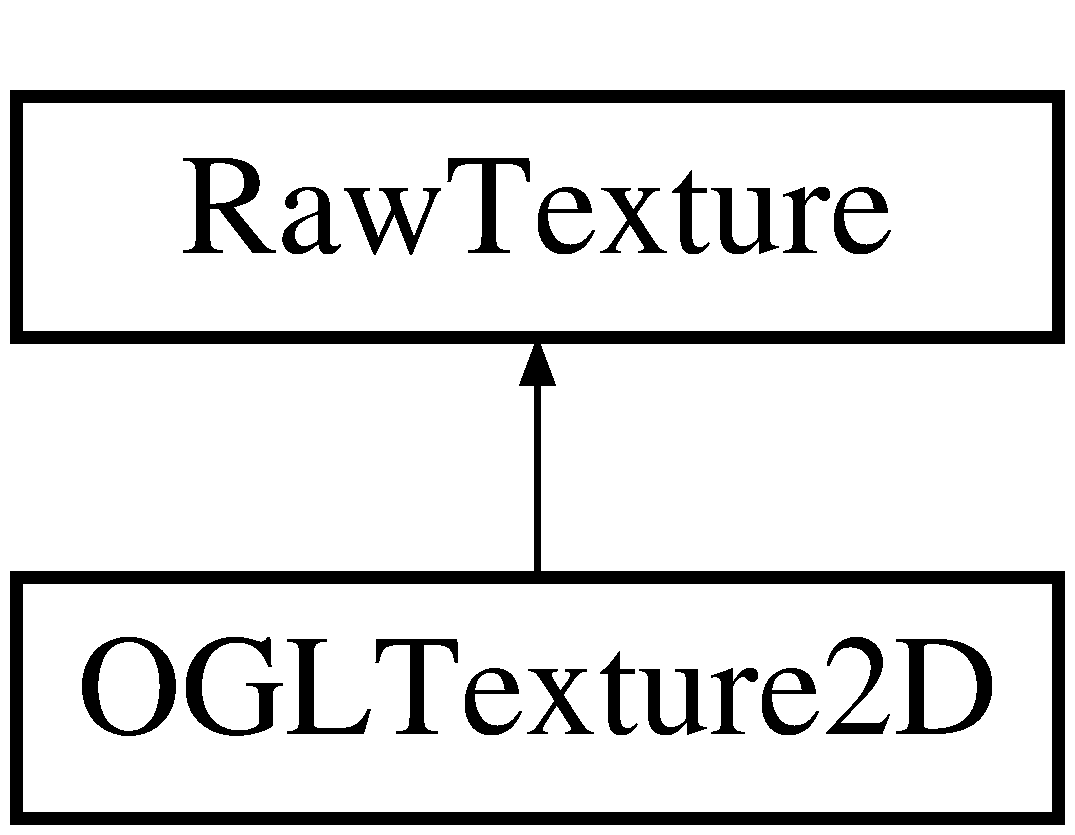
\includegraphics[height=2.000000cm]{class_o_g_l_texture2_d}
\end{center}
\end{figure}
\subsection*{Public Types}
\begin{DoxyCompactItemize}
\item 
enum \hyperlink{class_o_g_l_texture2_d_a853053ed9bf1c5e1024f947303cb0ec3}{Min\+Filter} \+: unsigned int \{ \\*
\hyperlink{class_o_g_l_texture2_d_a853053ed9bf1c5e1024f947303cb0ec3a60494f02d440f316319dd0fad40ad007}{Min\+Filter\+::\+Nearest} = (unsigned int)oglplus\+:\+:Texture\+Min\+Filter\+:\+:Nearest, 
\hyperlink{class_o_g_l_texture2_d_a853053ed9bf1c5e1024f947303cb0ec3a32a843da6ea40ab3b17a3421ccdf671b}{Min\+Filter\+::\+Linear} = (unsigned int)oglplus\+:\+:Texture\+Min\+Filter\+:\+:Linear, 
\hyperlink{class_o_g_l_texture2_d_a853053ed9bf1c5e1024f947303cb0ec3a35d97e4a37fa3a0d76c692f3e318599b}{Min\+Filter\+::\+Nearest\+Mipmap\+Nearest} = (unsigned int)oglplus\+:\+:Texture\+Min\+Filter\+:\+:Nearest\+Mipmap\+Nearest, 
\hyperlink{class_o_g_l_texture2_d_a853053ed9bf1c5e1024f947303cb0ec3ac164897273ad7f6d61626f5610d86425}{Min\+Filter\+::\+Linear\+Mipmap\+Nearest} = (unsigned int)oglplus\+:\+:Texture\+Min\+Filter\+:\+:Linear\+Mipmap\+Nearest, 
\\*
\hyperlink{class_o_g_l_texture2_d_a853053ed9bf1c5e1024f947303cb0ec3a9a79df5c07e4d2a2875689f608b50529}{Min\+Filter\+::\+Nearest\+Mipmap\+Linear} = (unsigned int)oglplus\+:\+:Texture\+Min\+Filter\+:\+:Nearest\+Mipmap\+Linear, 
\hyperlink{class_o_g_l_texture2_d_a853053ed9bf1c5e1024f947303cb0ec3a1173bd3987b1e185d86b9c3fe1b8bd72}{Min\+Filter\+::\+Linear\+Mipmap\+Linear} = (unsigned int)oglplus\+:\+:Texture\+Min\+Filter\+:\+:Linear\+Mipmap\+Linear
 \}
\item 
enum \hyperlink{class_o_g_l_texture2_d_ad72001307eaec4898b25c749c1857f25}{Mag\+Filter} \+: unsigned int \{ \hyperlink{class_o_g_l_texture2_d_ad72001307eaec4898b25c749c1857f25a60494f02d440f316319dd0fad40ad007}{Mag\+Filter\+::\+Nearest} = (unsigned int)oglplus\+:\+:Texture\+Mag\+Filter\+:\+:Nearest, 
\hyperlink{class_o_g_l_texture2_d_ad72001307eaec4898b25c749c1857f25a32a843da6ea40ab3b17a3421ccdf671b}{Mag\+Filter\+::\+Linear} = (unsigned int)oglplus\+:\+:Texture\+Mag\+Filter\+:\+:Linear
 \}
\item 
enum \hyperlink{class_o_g_l_texture2_d_ac6dae14737ed8643d30026dceebd10cc}{Wrap\+Mode} \+: unsigned int \{ \hyperlink{class_o_g_l_texture2_d_ac6dae14737ed8643d30026dceebd10cca7020426cfb0a204051be4b3053d2acc8}{Wrap\+Mode\+::\+Repeat} = (unsigned int)oglplus\+:\+:Texture\+Wrap\+:\+:Repeat, 
\hyperlink{class_o_g_l_texture2_d_ac6dae14737ed8643d30026dceebd10cca12ce4a5977988214a6b098b8cb0bf695}{Wrap\+Mode\+::\+Mirrored\+Repeat} = (unsigned int)oglplus\+:\+:Texture\+Wrap\+:\+:Mirrored\+Repeat, 
\hyperlink{class_o_g_l_texture2_d_ac6dae14737ed8643d30026dceebd10cca74556551231333c36debc3d373261134}{Wrap\+Mode\+::\+Clamp\+To\+Edge} = (unsigned int)oglplus\+:\+:Texture\+Wrap\+:\+:Clamp\+To\+Edge, 
\hyperlink{class_o_g_l_texture2_d_ac6dae14737ed8643d30026dceebd10ccafb07f88f6f11cc5ab9c951290716f147}{Wrap\+Mode\+::\+Clamp\+To\+Border} = (unsigned int)oglplus\+:\+:Texture\+Wrap\+:\+:Clamp\+To\+Border
 \}
\end{DoxyCompactItemize}
\subsection*{Public Member Functions}
\begin{DoxyCompactItemize}
\item 
\hyperlink{class_o_g_l_texture2_d_a5f3587a49e018d390c9474e89d9ae15e}{O\+G\+L\+Texture2\+D} ()
\item 
virtual \hyperlink{class_o_g_l_texture2_d_a2e6d4cd96428f3f85485f9d1fd311c80}{$\sim$\+O\+G\+L\+Texture2\+D} ()
\item 
G\+Luint \hyperlink{class_o_g_l_texture2_d_aceb3c2fe81ee4137fbf412def59c449e}{Upload\+To\+G\+P\+U} (\hyperlink{class_o_g_l_texture2_d_a853053ed9bf1c5e1024f947303cb0ec3}{Min\+Filter} \hyperlink{class_o_g_l_texture2_d_a064aa8eb5f6a5bc10300c0a68fd95c10}{min\+Filter}=\hyperlink{class_o_g_l_texture2_d_a853053ed9bf1c5e1024f947303cb0ec3a1173bd3987b1e185d86b9c3fe1b8bd72}{Min\+Filter\+::\+Linear\+Mipmap\+Linear}, \hyperlink{class_o_g_l_texture2_d_ad72001307eaec4898b25c749c1857f25}{Mag\+Filter} \hyperlink{class_o_g_l_texture2_d_abcc4f2fdc77667a1ff83d0f23b94fbdd}{mag\+Filter}=\hyperlink{class_o_g_l_texture2_d_ad72001307eaec4898b25c749c1857f25a32a843da6ea40ab3b17a3421ccdf671b}{Mag\+Filter\+::\+Linear}, \hyperlink{class_o_g_l_texture2_d_ac6dae14737ed8643d30026dceebd10cc}{Wrap\+Mode} \hyperlink{class_o_g_l_texture2_d_a9ce6cda4bc4c3149447c20017c35efd8}{wrap\+S}=\hyperlink{class_o_g_l_texture2_d_ac6dae14737ed8643d30026dceebd10cca7020426cfb0a204051be4b3053d2acc8}{Wrap\+Mode\+::\+Repeat}, \hyperlink{class_o_g_l_texture2_d_ac6dae14737ed8643d30026dceebd10cc}{Wrap\+Mode} \hyperlink{class_o_g_l_texture2_d_a66d477be8c69a34eb6dc5660926bf28f}{wrap\+T}=\hyperlink{class_o_g_l_texture2_d_ac6dae14737ed8643d30026dceebd10cca7020426cfb0a204051be4b3053d2acc8}{Wrap\+Mode\+::\+Repeat}, bool unload\+From\+R\+A\+M=true, bool generate\+Mipmaps=true, glm\+::vec4 \hyperlink{class_o_g_l_texture2_d_ab49fd4b19ab6b299d99c128b90861e9d}{border\+Color}=glm\+::vec4(0.f))
\item 
bool \hyperlink{class_o_g_l_texture2_d_aaae8e4366b6a604aefe29a084c829b40}{On\+G\+P\+U\+Memory} () const 
\item 
void \hyperlink{class_o_g_l_texture2_d_a847cee596365faa58b86887a24384402}{Bind} ()
\item 
int \hyperlink{class_o_g_l_texture2_d_a565bb9c1091b837eb319f90dd47bae8d}{Name} ()
\end{DoxyCompactItemize}
\subsection*{Static Public Member Functions}
\begin{DoxyCompactItemize}
\item 
static std\+::unique\+\_\+ptr$<$ \hyperlink{class_o_g_l_texture2_d}{O\+G\+L\+Texture2\+D} $>$ \& \hyperlink{class_o_g_l_texture2_d_aeb3f3e851142bc49196052fb1d5d08dc}{Get\+Default\+Texture} ()
\item 
static std\+::unique\+\_\+ptr$<$ \hyperlink{class_o_g_l_texture2_d}{O\+G\+L\+Texture2\+D} $>$ \& \hyperlink{class_o_g_l_texture2_d_a04fd79abfd27a237fb33fc4a16c4fb80}{Get\+Default\+Normal\+Texture} ()
\item 
static std\+::unique\+\_\+ptr$<$ \hyperlink{class_o_g_l_texture2_d}{O\+G\+L\+Texture2\+D} $>$ \& \hyperlink{class_o_g_l_texture2_d_a928c3129e954a9e11f6436286a95c1a0}{Get\+Error\+Texture} ()
\end{DoxyCompactItemize}
\subsection*{Static Protected Member Functions}
\begin{DoxyCompactItemize}
\item 
static \hyperlink{class_o_g_l_texture2_d}{O\+G\+L\+Texture2\+D} $\ast$ \hyperlink{class_o_g_l_texture2_d_ac6df286dd7a9c8a51393106fc49f2138}{Create\+Color\+Texture} (std\+::string tex\+Name, glm\+::u8vec3 tex\+Color)
\end{DoxyCompactItemize}
\subsection*{Protected Attributes}
\begin{DoxyCompactItemize}
\item 
std\+::unique\+\_\+ptr$<$ oglplus\+::\+Texture $>$ \hyperlink{class_o_g_l_texture2_d_a81c34266417bac598a6dcf78655e3657}{ogl\+Texture}
\item 
bool \hyperlink{class_o_g_l_texture2_d_ad0f35d77499d646cee162e9a3213c243}{mipmap\+Generated}
\item 
glm\+::vec4 \hyperlink{class_o_g_l_texture2_d_ab49fd4b19ab6b299d99c128b90861e9d}{border\+Color}
\item 
\hyperlink{class_o_g_l_texture2_d_ad72001307eaec4898b25c749c1857f25}{Mag\+Filter} \hyperlink{class_o_g_l_texture2_d_abcc4f2fdc77667a1ff83d0f23b94fbdd}{mag\+Filter}
\item 
\hyperlink{class_o_g_l_texture2_d_a853053ed9bf1c5e1024f947303cb0ec3}{Min\+Filter} \hyperlink{class_o_g_l_texture2_d_a064aa8eb5f6a5bc10300c0a68fd95c10}{min\+Filter}
\item 
\hyperlink{class_o_g_l_texture2_d_ac6dae14737ed8643d30026dceebd10cc}{Wrap\+Mode} \hyperlink{class_o_g_l_texture2_d_a9ce6cda4bc4c3149447c20017c35efd8}{wrap\+S}
\item 
\hyperlink{class_o_g_l_texture2_d_ac6dae14737ed8643d30026dceebd10cc}{Wrap\+Mode} \hyperlink{class_o_g_l_texture2_d_a66d477be8c69a34eb6dc5660926bf28f}{wrap\+T}
\item 
bool \hyperlink{class_o_g_l_texture2_d_a986498afd6ef99ef2bfc05b62a4c5b8b}{on\+G\+P\+U\+Memory}
\end{DoxyCompactItemize}
\subsection*{Static Protected Attributes}
\begin{DoxyCompactItemize}
\item 
static oglplus\+::\+Context \hyperlink{class_o_g_l_texture2_d_a53d4b615b88288938afb52730022d6a8}{gl}
\end{DoxyCompactItemize}
\subsection*{Additional Inherited Members}


\subsection{Detailed Description}


Definition at line 53 of file texture.\+h.



\subsection{Member Enumeration Documentation}
\hypertarget{class_o_g_l_texture2_d_ad72001307eaec4898b25c749c1857f25}{}\index{O\+G\+L\+Texture2\+D@{O\+G\+L\+Texture2\+D}!Mag\+Filter@{Mag\+Filter}}
\index{Mag\+Filter@{Mag\+Filter}!O\+G\+L\+Texture2\+D@{O\+G\+L\+Texture2\+D}}
\subsubsection[{Mag\+Filter}]{\setlength{\rightskip}{0pt plus 5cm}enum {\bf O\+G\+L\+Texture2\+D\+::\+Mag\+Filter} \+: unsigned int\hspace{0.3cm}{\ttfamily [strong]}}\label{class_o_g_l_texture2_d_ad72001307eaec4898b25c749c1857f25}
\begin{Desc}
\item[Enumerator]\par
\begin{description}
\index{Nearest@{Nearest}!O\+G\+L\+Texture2\+D@{O\+G\+L\+Texture2\+D}}\index{O\+G\+L\+Texture2\+D@{O\+G\+L\+Texture2\+D}!Nearest@{Nearest}}\item[{\em 
\hypertarget{class_o_g_l_texture2_d_ad72001307eaec4898b25c749c1857f25a60494f02d440f316319dd0fad40ad007}{}Nearest\label{class_o_g_l_texture2_d_ad72001307eaec4898b25c749c1857f25a60494f02d440f316319dd0fad40ad007}
}]\index{Linear@{Linear}!O\+G\+L\+Texture2\+D@{O\+G\+L\+Texture2\+D}}\index{O\+G\+L\+Texture2\+D@{O\+G\+L\+Texture2\+D}!Linear@{Linear}}\item[{\em 
\hypertarget{class_o_g_l_texture2_d_ad72001307eaec4898b25c749c1857f25a32a843da6ea40ab3b17a3421ccdf671b}{}Linear\label{class_o_g_l_texture2_d_ad72001307eaec4898b25c749c1857f25a32a843da6ea40ab3b17a3421ccdf671b}
}]\end{description}
\end{Desc}


Definition at line 66 of file texture.\+h.

\hypertarget{class_o_g_l_texture2_d_a853053ed9bf1c5e1024f947303cb0ec3}{}\index{O\+G\+L\+Texture2\+D@{O\+G\+L\+Texture2\+D}!Min\+Filter@{Min\+Filter}}
\index{Min\+Filter@{Min\+Filter}!O\+G\+L\+Texture2\+D@{O\+G\+L\+Texture2\+D}}
\subsubsection[{Min\+Filter}]{\setlength{\rightskip}{0pt plus 5cm}enum {\bf O\+G\+L\+Texture2\+D\+::\+Min\+Filter} \+: unsigned int\hspace{0.3cm}{\ttfamily [strong]}}\label{class_o_g_l_texture2_d_a853053ed9bf1c5e1024f947303cb0ec3}
\begin{Desc}
\item[Enumerator]\par
\begin{description}
\index{Nearest@{Nearest}!O\+G\+L\+Texture2\+D@{O\+G\+L\+Texture2\+D}}\index{O\+G\+L\+Texture2\+D@{O\+G\+L\+Texture2\+D}!Nearest@{Nearest}}\item[{\em 
\hypertarget{class_o_g_l_texture2_d_a853053ed9bf1c5e1024f947303cb0ec3a60494f02d440f316319dd0fad40ad007}{}Nearest\label{class_o_g_l_texture2_d_a853053ed9bf1c5e1024f947303cb0ec3a60494f02d440f316319dd0fad40ad007}
}]\index{Linear@{Linear}!O\+G\+L\+Texture2\+D@{O\+G\+L\+Texture2\+D}}\index{O\+G\+L\+Texture2\+D@{O\+G\+L\+Texture2\+D}!Linear@{Linear}}\item[{\em 
\hypertarget{class_o_g_l_texture2_d_a853053ed9bf1c5e1024f947303cb0ec3a32a843da6ea40ab3b17a3421ccdf671b}{}Linear\label{class_o_g_l_texture2_d_a853053ed9bf1c5e1024f947303cb0ec3a32a843da6ea40ab3b17a3421ccdf671b}
}]\index{Nearest\+Mipmap\+Nearest@{Nearest\+Mipmap\+Nearest}!O\+G\+L\+Texture2\+D@{O\+G\+L\+Texture2\+D}}\index{O\+G\+L\+Texture2\+D@{O\+G\+L\+Texture2\+D}!Nearest\+Mipmap\+Nearest@{Nearest\+Mipmap\+Nearest}}\item[{\em 
\hypertarget{class_o_g_l_texture2_d_a853053ed9bf1c5e1024f947303cb0ec3a35d97e4a37fa3a0d76c692f3e318599b}{}Nearest\+Mipmap\+Nearest\label{class_o_g_l_texture2_d_a853053ed9bf1c5e1024f947303cb0ec3a35d97e4a37fa3a0d76c692f3e318599b}
}]\index{Linear\+Mipmap\+Nearest@{Linear\+Mipmap\+Nearest}!O\+G\+L\+Texture2\+D@{O\+G\+L\+Texture2\+D}}\index{O\+G\+L\+Texture2\+D@{O\+G\+L\+Texture2\+D}!Linear\+Mipmap\+Nearest@{Linear\+Mipmap\+Nearest}}\item[{\em 
\hypertarget{class_o_g_l_texture2_d_a853053ed9bf1c5e1024f947303cb0ec3ac164897273ad7f6d61626f5610d86425}{}Linear\+Mipmap\+Nearest\label{class_o_g_l_texture2_d_a853053ed9bf1c5e1024f947303cb0ec3ac164897273ad7f6d61626f5610d86425}
}]\index{Nearest\+Mipmap\+Linear@{Nearest\+Mipmap\+Linear}!O\+G\+L\+Texture2\+D@{O\+G\+L\+Texture2\+D}}\index{O\+G\+L\+Texture2\+D@{O\+G\+L\+Texture2\+D}!Nearest\+Mipmap\+Linear@{Nearest\+Mipmap\+Linear}}\item[{\em 
\hypertarget{class_o_g_l_texture2_d_a853053ed9bf1c5e1024f947303cb0ec3a9a79df5c07e4d2a2875689f608b50529}{}Nearest\+Mipmap\+Linear\label{class_o_g_l_texture2_d_a853053ed9bf1c5e1024f947303cb0ec3a9a79df5c07e4d2a2875689f608b50529}
}]\index{Linear\+Mipmap\+Linear@{Linear\+Mipmap\+Linear}!O\+G\+L\+Texture2\+D@{O\+G\+L\+Texture2\+D}}\index{O\+G\+L\+Texture2\+D@{O\+G\+L\+Texture2\+D}!Linear\+Mipmap\+Linear@{Linear\+Mipmap\+Linear}}\item[{\em 
\hypertarget{class_o_g_l_texture2_d_a853053ed9bf1c5e1024f947303cb0ec3a1173bd3987b1e185d86b9c3fe1b8bd72}{}Linear\+Mipmap\+Linear\label{class_o_g_l_texture2_d_a853053ed9bf1c5e1024f947303cb0ec3a1173bd3987b1e185d86b9c3fe1b8bd72}
}]\end{description}
\end{Desc}


Definition at line 56 of file texture.\+h.

\hypertarget{class_o_g_l_texture2_d_ac6dae14737ed8643d30026dceebd10cc}{}\index{O\+G\+L\+Texture2\+D@{O\+G\+L\+Texture2\+D}!Wrap\+Mode@{Wrap\+Mode}}
\index{Wrap\+Mode@{Wrap\+Mode}!O\+G\+L\+Texture2\+D@{O\+G\+L\+Texture2\+D}}
\subsubsection[{Wrap\+Mode}]{\setlength{\rightskip}{0pt plus 5cm}enum {\bf O\+G\+L\+Texture2\+D\+::\+Wrap\+Mode} \+: unsigned int\hspace{0.3cm}{\ttfamily [strong]}}\label{class_o_g_l_texture2_d_ac6dae14737ed8643d30026dceebd10cc}
\begin{Desc}
\item[Enumerator]\par
\begin{description}
\index{Repeat@{Repeat}!O\+G\+L\+Texture2\+D@{O\+G\+L\+Texture2\+D}}\index{O\+G\+L\+Texture2\+D@{O\+G\+L\+Texture2\+D}!Repeat@{Repeat}}\item[{\em 
\hypertarget{class_o_g_l_texture2_d_ac6dae14737ed8643d30026dceebd10cca7020426cfb0a204051be4b3053d2acc8}{}Repeat\label{class_o_g_l_texture2_d_ac6dae14737ed8643d30026dceebd10cca7020426cfb0a204051be4b3053d2acc8}
}]\index{Mirrored\+Repeat@{Mirrored\+Repeat}!O\+G\+L\+Texture2\+D@{O\+G\+L\+Texture2\+D}}\index{O\+G\+L\+Texture2\+D@{O\+G\+L\+Texture2\+D}!Mirrored\+Repeat@{Mirrored\+Repeat}}\item[{\em 
\hypertarget{class_o_g_l_texture2_d_ac6dae14737ed8643d30026dceebd10cca12ce4a5977988214a6b098b8cb0bf695}{}Mirrored\+Repeat\label{class_o_g_l_texture2_d_ac6dae14737ed8643d30026dceebd10cca12ce4a5977988214a6b098b8cb0bf695}
}]\index{Clamp\+To\+Edge@{Clamp\+To\+Edge}!O\+G\+L\+Texture2\+D@{O\+G\+L\+Texture2\+D}}\index{O\+G\+L\+Texture2\+D@{O\+G\+L\+Texture2\+D}!Clamp\+To\+Edge@{Clamp\+To\+Edge}}\item[{\em 
\hypertarget{class_o_g_l_texture2_d_ac6dae14737ed8643d30026dceebd10cca74556551231333c36debc3d373261134}{}Clamp\+To\+Edge\label{class_o_g_l_texture2_d_ac6dae14737ed8643d30026dceebd10cca74556551231333c36debc3d373261134}
}]\index{Clamp\+To\+Border@{Clamp\+To\+Border}!O\+G\+L\+Texture2\+D@{O\+G\+L\+Texture2\+D}}\index{O\+G\+L\+Texture2\+D@{O\+G\+L\+Texture2\+D}!Clamp\+To\+Border@{Clamp\+To\+Border}}\item[{\em 
\hypertarget{class_o_g_l_texture2_d_ac6dae14737ed8643d30026dceebd10ccafb07f88f6f11cc5ab9c951290716f147}{}Clamp\+To\+Border\label{class_o_g_l_texture2_d_ac6dae14737ed8643d30026dceebd10ccafb07f88f6f11cc5ab9c951290716f147}
}]\end{description}
\end{Desc}


Definition at line 72 of file texture.\+h.



\subsection{Constructor \& Destructor Documentation}
\hypertarget{class_o_g_l_texture2_d_a5f3587a49e018d390c9474e89d9ae15e}{}\index{O\+G\+L\+Texture2\+D@{O\+G\+L\+Texture2\+D}!O\+G\+L\+Texture2\+D@{O\+G\+L\+Texture2\+D}}
\index{O\+G\+L\+Texture2\+D@{O\+G\+L\+Texture2\+D}!O\+G\+L\+Texture2\+D@{O\+G\+L\+Texture2\+D}}
\subsubsection[{O\+G\+L\+Texture2\+D()}]{\setlength{\rightskip}{0pt plus 5cm}O\+G\+L\+Texture2\+D\+::\+O\+G\+L\+Texture2\+D (
\begin{DoxyParamCaption}
{}
\end{DoxyParamCaption}
)}\label{class_o_g_l_texture2_d_a5f3587a49e018d390c9474e89d9ae15e}


Definition at line 165 of file texture.\+cpp.

\hypertarget{class_o_g_l_texture2_d_a2e6d4cd96428f3f85485f9d1fd311c80}{}\index{O\+G\+L\+Texture2\+D@{O\+G\+L\+Texture2\+D}!````~O\+G\+L\+Texture2\+D@{$\sim$\+O\+G\+L\+Texture2\+D}}
\index{````~O\+G\+L\+Texture2\+D@{$\sim$\+O\+G\+L\+Texture2\+D}!O\+G\+L\+Texture2\+D@{O\+G\+L\+Texture2\+D}}
\subsubsection[{$\sim$\+O\+G\+L\+Texture2\+D()}]{\setlength{\rightskip}{0pt plus 5cm}O\+G\+L\+Texture2\+D\+::$\sim$\+O\+G\+L\+Texture2\+D (
\begin{DoxyParamCaption}
{}
\end{DoxyParamCaption}
)\hspace{0.3cm}{\ttfamily [virtual]}}\label{class_o_g_l_texture2_d_a2e6d4cd96428f3f85485f9d1fd311c80}


Definition at line 169 of file texture.\+cpp.



\subsection{Member Function Documentation}
\hypertarget{class_o_g_l_texture2_d_a847cee596365faa58b86887a24384402}{}\index{O\+G\+L\+Texture2\+D@{O\+G\+L\+Texture2\+D}!Bind@{Bind}}
\index{Bind@{Bind}!O\+G\+L\+Texture2\+D@{O\+G\+L\+Texture2\+D}}
\subsubsection[{Bind()}]{\setlength{\rightskip}{0pt plus 5cm}void O\+G\+L\+Texture2\+D\+::\+Bind (
\begin{DoxyParamCaption}
{}
\end{DoxyParamCaption}
)}\label{class_o_g_l_texture2_d_a847cee596365faa58b86887a24384402}


Definition at line 86 of file texture.\+cpp.

\hypertarget{class_o_g_l_texture2_d_ac6df286dd7a9c8a51393106fc49f2138}{}\index{O\+G\+L\+Texture2\+D@{O\+G\+L\+Texture2\+D}!Create\+Color\+Texture@{Create\+Color\+Texture}}
\index{Create\+Color\+Texture@{Create\+Color\+Texture}!O\+G\+L\+Texture2\+D@{O\+G\+L\+Texture2\+D}}
\subsubsection[{Create\+Color\+Texture(std\+::string tex\+Name, glm\+::u8vec3 tex\+Color)}]{\setlength{\rightskip}{0pt plus 5cm}{\bf O\+G\+L\+Texture2\+D} $\ast$ O\+G\+L\+Texture2\+D\+::\+Create\+Color\+Texture (
\begin{DoxyParamCaption}
\item[{std\+::string}]{tex\+Name, }
\item[{glm\+::u8vec3}]{tex\+Color}
\end{DoxyParamCaption}
)\hspace{0.3cm}{\ttfamily [static]}, {\ttfamily [protected]}}\label{class_o_g_l_texture2_d_ac6df286dd7a9c8a51393106fc49f2138}


Definition at line 91 of file texture.\+cpp.

\hypertarget{class_o_g_l_texture2_d_a04fd79abfd27a237fb33fc4a16c4fb80}{}\index{O\+G\+L\+Texture2\+D@{O\+G\+L\+Texture2\+D}!Get\+Default\+Normal\+Texture@{Get\+Default\+Normal\+Texture}}
\index{Get\+Default\+Normal\+Texture@{Get\+Default\+Normal\+Texture}!O\+G\+L\+Texture2\+D@{O\+G\+L\+Texture2\+D}}
\subsubsection[{Get\+Default\+Normal\+Texture()}]{\setlength{\rightskip}{0pt plus 5cm}std\+::unique\+\_\+ptr$<$ {\bf O\+G\+L\+Texture2\+D} $>$ \& O\+G\+L\+Texture2\+D\+::\+Get\+Default\+Normal\+Texture (
\begin{DoxyParamCaption}
{}
\end{DoxyParamCaption}
)\hspace{0.3cm}{\ttfamily [static]}}\label{class_o_g_l_texture2_d_a04fd79abfd27a237fb33fc4a16c4fb80}


Definition at line 131 of file texture.\+cpp.

\hypertarget{class_o_g_l_texture2_d_aeb3f3e851142bc49196052fb1d5d08dc}{}\index{O\+G\+L\+Texture2\+D@{O\+G\+L\+Texture2\+D}!Get\+Default\+Texture@{Get\+Default\+Texture}}
\index{Get\+Default\+Texture@{Get\+Default\+Texture}!O\+G\+L\+Texture2\+D@{O\+G\+L\+Texture2\+D}}
\subsubsection[{Get\+Default\+Texture()}]{\setlength{\rightskip}{0pt plus 5cm}std\+::unique\+\_\+ptr$<$ {\bf O\+G\+L\+Texture2\+D} $>$ \& O\+G\+L\+Texture2\+D\+::\+Get\+Default\+Texture (
\begin{DoxyParamCaption}
{}
\end{DoxyParamCaption}
)\hspace{0.3cm}{\ttfamily [static]}}\label{class_o_g_l_texture2_d_aeb3f3e851142bc49196052fb1d5d08dc}


Definition at line 114 of file texture.\+cpp.

\hypertarget{class_o_g_l_texture2_d_a928c3129e954a9e11f6436286a95c1a0}{}\index{O\+G\+L\+Texture2\+D@{O\+G\+L\+Texture2\+D}!Get\+Error\+Texture@{Get\+Error\+Texture}}
\index{Get\+Error\+Texture@{Get\+Error\+Texture}!O\+G\+L\+Texture2\+D@{O\+G\+L\+Texture2\+D}}
\subsubsection[{Get\+Error\+Texture()}]{\setlength{\rightskip}{0pt plus 5cm}std\+::unique\+\_\+ptr$<$ {\bf O\+G\+L\+Texture2\+D} $>$ \& O\+G\+L\+Texture2\+D\+::\+Get\+Error\+Texture (
\begin{DoxyParamCaption}
{}
\end{DoxyParamCaption}
)\hspace{0.3cm}{\ttfamily [static]}}\label{class_o_g_l_texture2_d_a928c3129e954a9e11f6436286a95c1a0}


Definition at line 148 of file texture.\+cpp.

\hypertarget{class_o_g_l_texture2_d_a565bb9c1091b837eb319f90dd47bae8d}{}\index{O\+G\+L\+Texture2\+D@{O\+G\+L\+Texture2\+D}!Name@{Name}}
\index{Name@{Name}!O\+G\+L\+Texture2\+D@{O\+G\+L\+Texture2\+D}}
\subsubsection[{Name()}]{\setlength{\rightskip}{0pt plus 5cm}int O\+G\+L\+Texture2\+D\+::\+Name (
\begin{DoxyParamCaption}
{}
\end{DoxyParamCaption}
)\hspace{0.3cm}{\ttfamily [inline]}}\label{class_o_g_l_texture2_d_a565bb9c1091b837eb319f90dd47bae8d}


Definition at line 106 of file texture.\+h.

\hypertarget{class_o_g_l_texture2_d_aaae8e4366b6a604aefe29a084c829b40}{}\index{O\+G\+L\+Texture2\+D@{O\+G\+L\+Texture2\+D}!On\+G\+P\+U\+Memory@{On\+G\+P\+U\+Memory}}
\index{On\+G\+P\+U\+Memory@{On\+G\+P\+U\+Memory}!O\+G\+L\+Texture2\+D@{O\+G\+L\+Texture2\+D}}
\subsubsection[{On\+G\+P\+U\+Memory() const }]{\setlength{\rightskip}{0pt plus 5cm}bool O\+G\+L\+Texture2\+D\+::\+On\+G\+P\+U\+Memory (
\begin{DoxyParamCaption}
{}
\end{DoxyParamCaption}
) const\hspace{0.3cm}{\ttfamily [inline]}}\label{class_o_g_l_texture2_d_aaae8e4366b6a604aefe29a084c829b40}


Definition at line 104 of file texture.\+h.

\hypertarget{class_o_g_l_texture2_d_aceb3c2fe81ee4137fbf412def59c449e}{}\index{O\+G\+L\+Texture2\+D@{O\+G\+L\+Texture2\+D}!Upload\+To\+G\+P\+U@{Upload\+To\+G\+P\+U}}
\index{Upload\+To\+G\+P\+U@{Upload\+To\+G\+P\+U}!O\+G\+L\+Texture2\+D@{O\+G\+L\+Texture2\+D}}
\subsubsection[{Upload\+To\+G\+P\+U(\+Min\+Filter min\+Filter=\+Min\+Filter\+::\+Linear\+Mipmap\+Linear, Mag\+Filter mag\+Filter=\+Mag\+Filter\+::\+Linear, Wrap\+Mode wrap\+S=\+Wrap\+Mode\+::\+Repeat, Wrap\+Mode wrap\+T=\+Wrap\+Mode\+::\+Repeat, bool unload\+From\+R\+A\+M=true, bool generate\+Mipmaps=true, glm\+::vec4 border\+Color=glm\+::vec4(0.\+f))}]{\setlength{\rightskip}{0pt plus 5cm}G\+Luint O\+G\+L\+Texture2\+D\+::\+Upload\+To\+G\+P\+U (
\begin{DoxyParamCaption}
\item[{{\bf Min\+Filter}}]{min\+Filter = {\ttfamily {\bf Min\+Filter\+::\+Linear\+Mipmap\+Linear}}, }
\item[{{\bf Mag\+Filter}}]{mag\+Filter = {\ttfamily {\bf Mag\+Filter\+::\+Linear}}, }
\item[{{\bf Wrap\+Mode}}]{wrap\+S = {\ttfamily {\bf Wrap\+Mode\+::\+Repeat}}, }
\item[{{\bf Wrap\+Mode}}]{wrap\+T = {\ttfamily {\bf Wrap\+Mode\+::\+Repeat}}, }
\item[{bool}]{unload\+From\+R\+A\+M = {\ttfamily true}, }
\item[{bool}]{generate\+Mipmaps = {\ttfamily true}, }
\item[{glm\+::vec4}]{border\+Color = {\ttfamily glm\+:\+:vec4(0.f)}}
\end{DoxyParamCaption}
)}\label{class_o_g_l_texture2_d_aceb3c2fe81ee4137fbf412def59c449e}


Definition at line 22 of file texture.\+cpp.



\subsection{Member Data Documentation}
\hypertarget{class_o_g_l_texture2_d_ab49fd4b19ab6b299d99c128b90861e9d}{}\index{O\+G\+L\+Texture2\+D@{O\+G\+L\+Texture2\+D}!border\+Color@{border\+Color}}
\index{border\+Color@{border\+Color}!O\+G\+L\+Texture2\+D@{O\+G\+L\+Texture2\+D}}
\subsubsection[{border\+Color}]{\setlength{\rightskip}{0pt plus 5cm}glm\+::vec4 O\+G\+L\+Texture2\+D\+::border\+Color\hspace{0.3cm}{\ttfamily [protected]}}\label{class_o_g_l_texture2_d_ab49fd4b19ab6b299d99c128b90861e9d}


Definition at line 84 of file texture.\+h.

\hypertarget{class_o_g_l_texture2_d_a53d4b615b88288938afb52730022d6a8}{}\index{O\+G\+L\+Texture2\+D@{O\+G\+L\+Texture2\+D}!gl@{gl}}
\index{gl@{gl}!O\+G\+L\+Texture2\+D@{O\+G\+L\+Texture2\+D}}
\subsubsection[{gl}]{\setlength{\rightskip}{0pt plus 5cm}oglplus\+::\+Context O\+G\+L\+Texture2\+D\+::gl\hspace{0.3cm}{\ttfamily [static]}, {\ttfamily [protected]}}\label{class_o_g_l_texture2_d_a53d4b615b88288938afb52730022d6a8}


Definition at line 80 of file texture.\+h.

\hypertarget{class_o_g_l_texture2_d_abcc4f2fdc77667a1ff83d0f23b94fbdd}{}\index{O\+G\+L\+Texture2\+D@{O\+G\+L\+Texture2\+D}!mag\+Filter@{mag\+Filter}}
\index{mag\+Filter@{mag\+Filter}!O\+G\+L\+Texture2\+D@{O\+G\+L\+Texture2\+D}}
\subsubsection[{mag\+Filter}]{\setlength{\rightskip}{0pt plus 5cm}{\bf Mag\+Filter} O\+G\+L\+Texture2\+D\+::mag\+Filter\hspace{0.3cm}{\ttfamily [protected]}}\label{class_o_g_l_texture2_d_abcc4f2fdc77667a1ff83d0f23b94fbdd}


Definition at line 85 of file texture.\+h.

\hypertarget{class_o_g_l_texture2_d_a064aa8eb5f6a5bc10300c0a68fd95c10}{}\index{O\+G\+L\+Texture2\+D@{O\+G\+L\+Texture2\+D}!min\+Filter@{min\+Filter}}
\index{min\+Filter@{min\+Filter}!O\+G\+L\+Texture2\+D@{O\+G\+L\+Texture2\+D}}
\subsubsection[{min\+Filter}]{\setlength{\rightskip}{0pt plus 5cm}{\bf Min\+Filter} O\+G\+L\+Texture2\+D\+::min\+Filter\hspace{0.3cm}{\ttfamily [protected]}}\label{class_o_g_l_texture2_d_a064aa8eb5f6a5bc10300c0a68fd95c10}


Definition at line 86 of file texture.\+h.

\hypertarget{class_o_g_l_texture2_d_ad0f35d77499d646cee162e9a3213c243}{}\index{O\+G\+L\+Texture2\+D@{O\+G\+L\+Texture2\+D}!mipmap\+Generated@{mipmap\+Generated}}
\index{mipmap\+Generated@{mipmap\+Generated}!O\+G\+L\+Texture2\+D@{O\+G\+L\+Texture2\+D}}
\subsubsection[{mipmap\+Generated}]{\setlength{\rightskip}{0pt plus 5cm}bool O\+G\+L\+Texture2\+D\+::mipmap\+Generated\hspace{0.3cm}{\ttfamily [protected]}}\label{class_o_g_l_texture2_d_ad0f35d77499d646cee162e9a3213c243}


Definition at line 83 of file texture.\+h.

\hypertarget{class_o_g_l_texture2_d_a81c34266417bac598a6dcf78655e3657}{}\index{O\+G\+L\+Texture2\+D@{O\+G\+L\+Texture2\+D}!ogl\+Texture@{ogl\+Texture}}
\index{ogl\+Texture@{ogl\+Texture}!O\+G\+L\+Texture2\+D@{O\+G\+L\+Texture2\+D}}
\subsubsection[{ogl\+Texture}]{\setlength{\rightskip}{0pt plus 5cm}std\+::unique\+\_\+ptr$<$oglplus\+::\+Texture$>$ O\+G\+L\+Texture2\+D\+::ogl\+Texture\hspace{0.3cm}{\ttfamily [protected]}}\label{class_o_g_l_texture2_d_a81c34266417bac598a6dcf78655e3657}


Definition at line 81 of file texture.\+h.

\hypertarget{class_o_g_l_texture2_d_a986498afd6ef99ef2bfc05b62a4c5b8b}{}\index{O\+G\+L\+Texture2\+D@{O\+G\+L\+Texture2\+D}!on\+G\+P\+U\+Memory@{on\+G\+P\+U\+Memory}}
\index{on\+G\+P\+U\+Memory@{on\+G\+P\+U\+Memory}!O\+G\+L\+Texture2\+D@{O\+G\+L\+Texture2\+D}}
\subsubsection[{on\+G\+P\+U\+Memory}]{\setlength{\rightskip}{0pt plus 5cm}bool O\+G\+L\+Texture2\+D\+::on\+G\+P\+U\+Memory\hspace{0.3cm}{\ttfamily [protected]}}\label{class_o_g_l_texture2_d_a986498afd6ef99ef2bfc05b62a4c5b8b}


Definition at line 90 of file texture.\+h.

\hypertarget{class_o_g_l_texture2_d_a9ce6cda4bc4c3149447c20017c35efd8}{}\index{O\+G\+L\+Texture2\+D@{O\+G\+L\+Texture2\+D}!wrap\+S@{wrap\+S}}
\index{wrap\+S@{wrap\+S}!O\+G\+L\+Texture2\+D@{O\+G\+L\+Texture2\+D}}
\subsubsection[{wrap\+S}]{\setlength{\rightskip}{0pt plus 5cm}{\bf Wrap\+Mode} O\+G\+L\+Texture2\+D\+::wrap\+S\hspace{0.3cm}{\ttfamily [protected]}}\label{class_o_g_l_texture2_d_a9ce6cda4bc4c3149447c20017c35efd8}


Definition at line 87 of file texture.\+h.

\hypertarget{class_o_g_l_texture2_d_a66d477be8c69a34eb6dc5660926bf28f}{}\index{O\+G\+L\+Texture2\+D@{O\+G\+L\+Texture2\+D}!wrap\+T@{wrap\+T}}
\index{wrap\+T@{wrap\+T}!O\+G\+L\+Texture2\+D@{O\+G\+L\+Texture2\+D}}
\subsubsection[{wrap\+T}]{\setlength{\rightskip}{0pt plus 5cm}{\bf Wrap\+Mode} O\+G\+L\+Texture2\+D\+::wrap\+T\hspace{0.3cm}{\ttfamily [protected]}}\label{class_o_g_l_texture2_d_a66d477be8c69a34eb6dc5660926bf28f}


Definition at line 88 of file texture.\+h.



The documentation for this class was generated from the following files\+:\begin{DoxyCompactItemize}
\item 
V\+C\+T\+\_\+\+Engine/scene/\hyperlink{texture_8h}{texture.\+h}\item 
V\+C\+T\+\_\+\+Engine/scene/\hyperlink{texture_8cpp}{texture.\+cpp}\end{DoxyCompactItemize}

\hypertarget{class_raw_texture}{}\section{Raw\+Texture Class Reference}
\label{class_raw_texture}\index{Raw\+Texture@{Raw\+Texture}}


{\ttfamily \#include $<$texture.\+h$>$}

Inheritance diagram for Raw\+Texture\+:\begin{figure}[H]
\begin{center}
\leavevmode
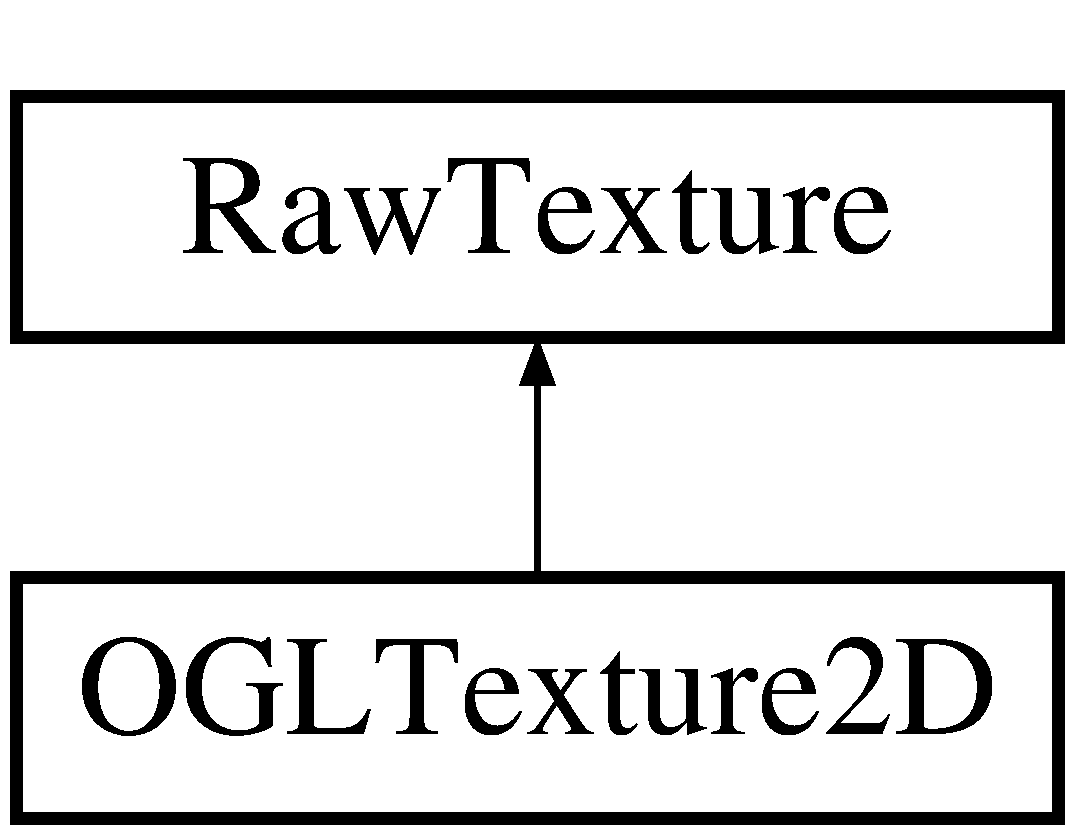
\includegraphics[height=2.000000cm]{class_raw_texture}
\end{center}
\end{figure}
\subsection*{Public Types}
\begin{DoxyCompactItemize}
\item 
enum \hyperlink{class_raw_texture_ac0eafe7206f7f38aeb4e8e5631480f6d}{Texture\+Type} \{ \\*
\hyperlink{class_raw_texture_ac0eafe7206f7f38aeb4e8e5631480f6da78fec4598173ba0ac7e88172f904bf14}{None}, 
\hyperlink{class_raw_texture_ac0eafe7206f7f38aeb4e8e5631480f6da103010e71865c656628def4a68509078}{Diffuse}, 
\hyperlink{class_raw_texture_ac0eafe7206f7f38aeb4e8e5631480f6da376419225ba86ef2cef8deaf4b5d2cc0}{Specular}, 
\hyperlink{class_raw_texture_ac0eafe7206f7f38aeb4e8e5631480f6dae40768618fb98d5bf8f8b508beee978d}{Ambient}, 
\\*
\hyperlink{class_raw_texture_ac0eafe7206f7f38aeb4e8e5631480f6da129d22adf6decce68912629eb9d86f4c}{Emissive}, 
\hyperlink{class_raw_texture_ac0eafe7206f7f38aeb4e8e5631480f6da36aa55c6d051efa1528323021dc6bfdb}{Height}, 
\hyperlink{class_raw_texture_ac0eafe7206f7f38aeb4e8e5631480f6da31db990e66434b96fc42213080e8aee5}{Normals}, 
\hyperlink{class_raw_texture_ac0eafe7206f7f38aeb4e8e5631480f6da22852ea63e2e64bdcda0650e6226bc8f}{Shininess}, 
\\*
\hyperlink{class_raw_texture_ac0eafe7206f7f38aeb4e8e5631480f6da578768bb075d4923ac61b46940c5fa83}{Opacity}, 
\hyperlink{class_raw_texture_ac0eafe7206f7f38aeb4e8e5631480f6da18c524764d6c9260aa6d2e140219c303}{Displacement}, 
\hyperlink{class_raw_texture_ac0eafe7206f7f38aeb4e8e5631480f6da5d61225d770ccb26dd0467db41c49c40}{Lightmap}, 
\hyperlink{class_raw_texture_ac0eafe7206f7f38aeb4e8e5631480f6daeb9ce3fdf067487fa1c3c543eadcb995}{Reflection}, 
\\*
\hyperlink{class_raw_texture_ac0eafe7206f7f38aeb4e8e5631480f6da80a818ecbfab54372aaa78f8eefff24e}{Unknow}, 
\hyperlink{class_raw_texture_ac0eafe7206f7f38aeb4e8e5631480f6daf629e42f84129e5f38c0b66b4887f09b}{T\+E\+X\+T\+U\+R\+E\+\_\+\+T\+Y\+P\+E\+\_\+\+M\+A\+X}
 \}
\end{DoxyCompactItemize}
\subsection*{Public Member Functions}
\begin{DoxyCompactItemize}
\item 
void \hyperlink{class_raw_texture_abc0bd100ec01cb31fd21dffb4a9dcab3}{Free\+Raw\+Data} ()
\item 
std\+::string \hyperlink{class_raw_texture_a481b8bb91a2218f802ad45ac9e9d9f77}{Get\+Filepath} () const 
\item 
\hyperlink{class_raw_texture_aaf66d9b0d654b8a2ddb02341aa660c52}{Raw\+Texture} ()
\item 
\hyperlink{class_raw_texture_a7d8603a772731a706575d2a4e42aca89}{$\sim$\+Raw\+Texture} ()
\end{DoxyCompactItemize}
\subsection*{Public Attributes}
\begin{DoxyCompactItemize}
\item 
std\+::set$<$ \hyperlink{class_raw_texture_ac0eafe7206f7f38aeb4e8e5631480f6d}{Texture\+Type} $>$ \hyperlink{class_raw_texture_a41f22696466ec5f4996f0f4dccc7e5e0}{texture\+Types}
\end{DoxyCompactItemize}
\subsection*{Protected Attributes}
\begin{DoxyCompactItemize}
\item 
std\+::string \hyperlink{class_raw_texture_a0f5f0ecaf7fd35c4fba96462d760aa0b}{filepath}
\item 
unsigned int \hyperlink{class_raw_texture_ac5e37bde9f359cb9676891d8636e75d0}{height}
\item 
unsigned int \hyperlink{class_raw_texture_a8db9a3ed2c3851077b13b881db99232c}{width}
\item 
unsigned int \hyperlink{class_raw_texture_abfd4db2756cc368282a55b1a6f8fc566}{depth}
\item 
unsigned int \hyperlink{class_raw_texture_a2bdb867781ad732469c7d03d9ce46f55}{line\+Width}
\item 
unsigned int \hyperlink{class_raw_texture_a30328bee28779a85b47f25886f1a3ff2}{bits\+Per\+Pixel}
\item 
std\+::unique\+\_\+ptr$<$ unsigned char $>$ \hyperlink{class_raw_texture_abe931dadd2a4b5bdbe82ee31f87ae60c}{raw\+Data}
\end{DoxyCompactItemize}
\subsection*{Friends}
\begin{DoxyCompactItemize}
\item 
class \hyperlink{class_raw_texture_a72d3411e09812d0e365245420a64c3ec}{Texture\+Importer}
\end{DoxyCompactItemize}


\subsection{Detailed Description}


Definition at line 3 of file texture.\+h.



\subsection{Member Enumeration Documentation}
\hypertarget{class_raw_texture_ac0eafe7206f7f38aeb4e8e5631480f6d}{}\index{Raw\+Texture@{Raw\+Texture}!Texture\+Type@{Texture\+Type}}
\index{Texture\+Type@{Texture\+Type}!Raw\+Texture@{Raw\+Texture}}
\subsubsection[{Texture\+Type}]{\setlength{\rightskip}{0pt plus 5cm}enum {\bf Raw\+Texture\+::\+Texture\+Type}}\label{class_raw_texture_ac0eafe7206f7f38aeb4e8e5631480f6d}
\begin{Desc}
\item[Enumerator]\par
\begin{description}
\index{None@{None}!Raw\+Texture@{Raw\+Texture}}\index{Raw\+Texture@{Raw\+Texture}!None@{None}}\item[{\em 
\hypertarget{class_raw_texture_ac0eafe7206f7f38aeb4e8e5631480f6da78fec4598173ba0ac7e88172f904bf14}{}None\label{class_raw_texture_ac0eafe7206f7f38aeb4e8e5631480f6da78fec4598173ba0ac7e88172f904bf14}
}]\index{Diffuse@{Diffuse}!Raw\+Texture@{Raw\+Texture}}\index{Raw\+Texture@{Raw\+Texture}!Diffuse@{Diffuse}}\item[{\em 
\hypertarget{class_raw_texture_ac0eafe7206f7f38aeb4e8e5631480f6da103010e71865c656628def4a68509078}{}Diffuse\label{class_raw_texture_ac0eafe7206f7f38aeb4e8e5631480f6da103010e71865c656628def4a68509078}
}]\index{Specular@{Specular}!Raw\+Texture@{Raw\+Texture}}\index{Raw\+Texture@{Raw\+Texture}!Specular@{Specular}}\item[{\em 
\hypertarget{class_raw_texture_ac0eafe7206f7f38aeb4e8e5631480f6da376419225ba86ef2cef8deaf4b5d2cc0}{}Specular\label{class_raw_texture_ac0eafe7206f7f38aeb4e8e5631480f6da376419225ba86ef2cef8deaf4b5d2cc0}
}]\index{Ambient@{Ambient}!Raw\+Texture@{Raw\+Texture}}\index{Raw\+Texture@{Raw\+Texture}!Ambient@{Ambient}}\item[{\em 
\hypertarget{class_raw_texture_ac0eafe7206f7f38aeb4e8e5631480f6dae40768618fb98d5bf8f8b508beee978d}{}Ambient\label{class_raw_texture_ac0eafe7206f7f38aeb4e8e5631480f6dae40768618fb98d5bf8f8b508beee978d}
}]\index{Emissive@{Emissive}!Raw\+Texture@{Raw\+Texture}}\index{Raw\+Texture@{Raw\+Texture}!Emissive@{Emissive}}\item[{\em 
\hypertarget{class_raw_texture_ac0eafe7206f7f38aeb4e8e5631480f6da129d22adf6decce68912629eb9d86f4c}{}Emissive\label{class_raw_texture_ac0eafe7206f7f38aeb4e8e5631480f6da129d22adf6decce68912629eb9d86f4c}
}]\index{Height@{Height}!Raw\+Texture@{Raw\+Texture}}\index{Raw\+Texture@{Raw\+Texture}!Height@{Height}}\item[{\em 
\hypertarget{class_raw_texture_ac0eafe7206f7f38aeb4e8e5631480f6da36aa55c6d051efa1528323021dc6bfdb}{}Height\label{class_raw_texture_ac0eafe7206f7f38aeb4e8e5631480f6da36aa55c6d051efa1528323021dc6bfdb}
}]\index{Normals@{Normals}!Raw\+Texture@{Raw\+Texture}}\index{Raw\+Texture@{Raw\+Texture}!Normals@{Normals}}\item[{\em 
\hypertarget{class_raw_texture_ac0eafe7206f7f38aeb4e8e5631480f6da31db990e66434b96fc42213080e8aee5}{}Normals\label{class_raw_texture_ac0eafe7206f7f38aeb4e8e5631480f6da31db990e66434b96fc42213080e8aee5}
}]\index{Shininess@{Shininess}!Raw\+Texture@{Raw\+Texture}}\index{Raw\+Texture@{Raw\+Texture}!Shininess@{Shininess}}\item[{\em 
\hypertarget{class_raw_texture_ac0eafe7206f7f38aeb4e8e5631480f6da22852ea63e2e64bdcda0650e6226bc8f}{}Shininess\label{class_raw_texture_ac0eafe7206f7f38aeb4e8e5631480f6da22852ea63e2e64bdcda0650e6226bc8f}
}]\index{Opacity@{Opacity}!Raw\+Texture@{Raw\+Texture}}\index{Raw\+Texture@{Raw\+Texture}!Opacity@{Opacity}}\item[{\em 
\hypertarget{class_raw_texture_ac0eafe7206f7f38aeb4e8e5631480f6da578768bb075d4923ac61b46940c5fa83}{}Opacity\label{class_raw_texture_ac0eafe7206f7f38aeb4e8e5631480f6da578768bb075d4923ac61b46940c5fa83}
}]\index{Displacement@{Displacement}!Raw\+Texture@{Raw\+Texture}}\index{Raw\+Texture@{Raw\+Texture}!Displacement@{Displacement}}\item[{\em 
\hypertarget{class_raw_texture_ac0eafe7206f7f38aeb4e8e5631480f6da18c524764d6c9260aa6d2e140219c303}{}Displacement\label{class_raw_texture_ac0eafe7206f7f38aeb4e8e5631480f6da18c524764d6c9260aa6d2e140219c303}
}]\index{Lightmap@{Lightmap}!Raw\+Texture@{Raw\+Texture}}\index{Raw\+Texture@{Raw\+Texture}!Lightmap@{Lightmap}}\item[{\em 
\hypertarget{class_raw_texture_ac0eafe7206f7f38aeb4e8e5631480f6da5d61225d770ccb26dd0467db41c49c40}{}Lightmap\label{class_raw_texture_ac0eafe7206f7f38aeb4e8e5631480f6da5d61225d770ccb26dd0467db41c49c40}
}]\index{Reflection@{Reflection}!Raw\+Texture@{Raw\+Texture}}\index{Raw\+Texture@{Raw\+Texture}!Reflection@{Reflection}}\item[{\em 
\hypertarget{class_raw_texture_ac0eafe7206f7f38aeb4e8e5631480f6daeb9ce3fdf067487fa1c3c543eadcb995}{}Reflection\label{class_raw_texture_ac0eafe7206f7f38aeb4e8e5631480f6daeb9ce3fdf067487fa1c3c543eadcb995}
}]\index{Unknow@{Unknow}!Raw\+Texture@{Raw\+Texture}}\index{Raw\+Texture@{Raw\+Texture}!Unknow@{Unknow}}\item[{\em 
\hypertarget{class_raw_texture_ac0eafe7206f7f38aeb4e8e5631480f6da80a818ecbfab54372aaa78f8eefff24e}{}Unknow\label{class_raw_texture_ac0eafe7206f7f38aeb4e8e5631480f6da80a818ecbfab54372aaa78f8eefff24e}
}]\index{T\+E\+X\+T\+U\+R\+E\+\_\+\+T\+Y\+P\+E\+\_\+\+M\+A\+X@{T\+E\+X\+T\+U\+R\+E\+\_\+\+T\+Y\+P\+E\+\_\+\+M\+A\+X}!Raw\+Texture@{Raw\+Texture}}\index{Raw\+Texture@{Raw\+Texture}!T\+E\+X\+T\+U\+R\+E\+\_\+\+T\+Y\+P\+E\+\_\+\+M\+A\+X@{T\+E\+X\+T\+U\+R\+E\+\_\+\+T\+Y\+P\+E\+\_\+\+M\+A\+X}}\item[{\em 
\hypertarget{class_raw_texture_ac0eafe7206f7f38aeb4e8e5631480f6daf629e42f84129e5f38c0b66b4887f09b}{}T\+E\+X\+T\+U\+R\+E\+\_\+\+T\+Y\+P\+E\+\_\+\+M\+A\+X\label{class_raw_texture_ac0eafe7206f7f38aeb4e8e5631480f6daf629e42f84129e5f38c0b66b4887f09b}
}]\end{description}
\end{Desc}


Definition at line 6 of file texture.\+h.



\subsection{Constructor \& Destructor Documentation}
\hypertarget{class_raw_texture_aaf66d9b0d654b8a2ddb02341aa660c52}{}\index{Raw\+Texture@{Raw\+Texture}!Raw\+Texture@{Raw\+Texture}}
\index{Raw\+Texture@{Raw\+Texture}!Raw\+Texture@{Raw\+Texture}}
\subsubsection[{Raw\+Texture()}]{\setlength{\rightskip}{0pt plus 5cm}Raw\+Texture\+::\+Raw\+Texture (
\begin{DoxyParamCaption}
{}
\end{DoxyParamCaption}
)}\label{class_raw_texture_aaf66d9b0d654b8a2ddb02341aa660c52}


Definition at line 12 of file texture.\+cpp.

\hypertarget{class_raw_texture_a7d8603a772731a706575d2a4e42aca89}{}\index{Raw\+Texture@{Raw\+Texture}!````~Raw\+Texture@{$\sim$\+Raw\+Texture}}
\index{````~Raw\+Texture@{$\sim$\+Raw\+Texture}!Raw\+Texture@{Raw\+Texture}}
\subsubsection[{$\sim$\+Raw\+Texture()}]{\setlength{\rightskip}{0pt plus 5cm}Raw\+Texture\+::$\sim$\+Raw\+Texture (
\begin{DoxyParamCaption}
{}
\end{DoxyParamCaption}
)}\label{class_raw_texture_a7d8603a772731a706575d2a4e42aca89}


Definition at line 17 of file texture.\+cpp.



\subsection{Member Function Documentation}
\hypertarget{class_raw_texture_abc0bd100ec01cb31fd21dffb4a9dcab3}{}\index{Raw\+Texture@{Raw\+Texture}!Free\+Raw\+Data@{Free\+Raw\+Data}}
\index{Free\+Raw\+Data@{Free\+Raw\+Data}!Raw\+Texture@{Raw\+Texture}}
\subsubsection[{Free\+Raw\+Data()}]{\setlength{\rightskip}{0pt plus 5cm}void Raw\+Texture\+::\+Free\+Raw\+Data (
\begin{DoxyParamCaption}
{}
\end{DoxyParamCaption}
)}\label{class_raw_texture_abc0bd100ec01cb31fd21dffb4a9dcab3}


Definition at line 4 of file texture.\+cpp.

\hypertarget{class_raw_texture_a481b8bb91a2218f802ad45ac9e9d9f77}{}\index{Raw\+Texture@{Raw\+Texture}!Get\+Filepath@{Get\+Filepath}}
\index{Get\+Filepath@{Get\+Filepath}!Raw\+Texture@{Raw\+Texture}}
\subsubsection[{Get\+Filepath() const }]{\setlength{\rightskip}{0pt plus 5cm}std\+::string Raw\+Texture\+::\+Get\+Filepath (
\begin{DoxyParamCaption}
{}
\end{DoxyParamCaption}
) const\hspace{0.3cm}{\ttfamily [inline]}}\label{class_raw_texture_a481b8bb91a2218f802ad45ac9e9d9f77}


Definition at line 28 of file texture.\+h.



\subsection{Friends And Related Function Documentation}
\hypertarget{class_raw_texture_a72d3411e09812d0e365245420a64c3ec}{}\index{Raw\+Texture@{Raw\+Texture}!Texture\+Importer@{Texture\+Importer}}
\index{Texture\+Importer@{Texture\+Importer}!Raw\+Texture@{Raw\+Texture}}
\subsubsection[{Texture\+Importer}]{\setlength{\rightskip}{0pt plus 5cm}friend class {\bf Texture\+Importer}\hspace{0.3cm}{\ttfamily [friend]}}\label{class_raw_texture_a72d3411e09812d0e365245420a64c3ec}


Definition at line 49 of file texture.\+h.



\subsection{Member Data Documentation}
\hypertarget{class_raw_texture_a30328bee28779a85b47f25886f1a3ff2}{}\index{Raw\+Texture@{Raw\+Texture}!bits\+Per\+Pixel@{bits\+Per\+Pixel}}
\index{bits\+Per\+Pixel@{bits\+Per\+Pixel}!Raw\+Texture@{Raw\+Texture}}
\subsubsection[{bits\+Per\+Pixel}]{\setlength{\rightskip}{0pt plus 5cm}unsigned int Raw\+Texture\+::bits\+Per\+Pixel\hspace{0.3cm}{\ttfamily [protected]}}\label{class_raw_texture_a30328bee28779a85b47f25886f1a3ff2}


Definition at line 37 of file texture.\+h.

\hypertarget{class_raw_texture_abfd4db2756cc368282a55b1a6f8fc566}{}\index{Raw\+Texture@{Raw\+Texture}!depth@{depth}}
\index{depth@{depth}!Raw\+Texture@{Raw\+Texture}}
\subsubsection[{depth}]{\setlength{\rightskip}{0pt plus 5cm}unsigned int Raw\+Texture\+::depth\hspace{0.3cm}{\ttfamily [protected]}}\label{class_raw_texture_abfd4db2756cc368282a55b1a6f8fc566}


Definition at line 34 of file texture.\+h.

\hypertarget{class_raw_texture_a0f5f0ecaf7fd35c4fba96462d760aa0b}{}\index{Raw\+Texture@{Raw\+Texture}!filepath@{filepath}}
\index{filepath@{filepath}!Raw\+Texture@{Raw\+Texture}}
\subsubsection[{filepath}]{\setlength{\rightskip}{0pt plus 5cm}std\+::string Raw\+Texture\+::filepath\hspace{0.3cm}{\ttfamily [protected]}}\label{class_raw_texture_a0f5f0ecaf7fd35c4fba96462d760aa0b}


Definition at line 30 of file texture.\+h.

\hypertarget{class_raw_texture_ac5e37bde9f359cb9676891d8636e75d0}{}\index{Raw\+Texture@{Raw\+Texture}!height@{height}}
\index{height@{height}!Raw\+Texture@{Raw\+Texture}}
\subsubsection[{height}]{\setlength{\rightskip}{0pt plus 5cm}unsigned int Raw\+Texture\+::height\hspace{0.3cm}{\ttfamily [protected]}}\label{class_raw_texture_ac5e37bde9f359cb9676891d8636e75d0}


Definition at line 32 of file texture.\+h.

\hypertarget{class_raw_texture_a2bdb867781ad732469c7d03d9ce46f55}{}\index{Raw\+Texture@{Raw\+Texture}!line\+Width@{line\+Width}}
\index{line\+Width@{line\+Width}!Raw\+Texture@{Raw\+Texture}}
\subsubsection[{line\+Width}]{\setlength{\rightskip}{0pt plus 5cm}unsigned int Raw\+Texture\+::line\+Width\hspace{0.3cm}{\ttfamily [protected]}}\label{class_raw_texture_a2bdb867781ad732469c7d03d9ce46f55}


Definition at line 36 of file texture.\+h.

\hypertarget{class_raw_texture_abe931dadd2a4b5bdbe82ee31f87ae60c}{}\index{Raw\+Texture@{Raw\+Texture}!raw\+Data@{raw\+Data}}
\index{raw\+Data@{raw\+Data}!Raw\+Texture@{Raw\+Texture}}
\subsubsection[{raw\+Data}]{\setlength{\rightskip}{0pt plus 5cm}std\+::unique\+\_\+ptr$<$unsigned char$>$ Raw\+Texture\+::raw\+Data\hspace{0.3cm}{\ttfamily [protected]}}\label{class_raw_texture_abe931dadd2a4b5bdbe82ee31f87ae60c}


Definition at line 39 of file texture.\+h.

\hypertarget{class_raw_texture_a41f22696466ec5f4996f0f4dccc7e5e0}{}\index{Raw\+Texture@{Raw\+Texture}!texture\+Types@{texture\+Types}}
\index{texture\+Types@{texture\+Types}!Raw\+Texture@{Raw\+Texture}}
\subsubsection[{texture\+Types}]{\setlength{\rightskip}{0pt plus 5cm}std\+::set$<${\bf Texture\+Type}$>$ Raw\+Texture\+::texture\+Types}\label{class_raw_texture_a41f22696466ec5f4996f0f4dccc7e5e0}


Definition at line 24 of file texture.\+h.

\hypertarget{class_raw_texture_a8db9a3ed2c3851077b13b881db99232c}{}\index{Raw\+Texture@{Raw\+Texture}!width@{width}}
\index{width@{width}!Raw\+Texture@{Raw\+Texture}}
\subsubsection[{width}]{\setlength{\rightskip}{0pt plus 5cm}unsigned int Raw\+Texture\+::width\hspace{0.3cm}{\ttfamily [protected]}}\label{class_raw_texture_a8db9a3ed2c3851077b13b881db99232c}


Definition at line 33 of file texture.\+h.



The documentation for this class was generated from the following files\+:\begin{DoxyCompactItemize}
\item 
V\+C\+T\+\_\+\+Engine/scene/\hyperlink{texture_8h}{texture.\+h}\item 
V\+C\+T\+\_\+\+Engine/scene/\hyperlink{texture_8cpp}{texture.\+cpp}\end{DoxyCompactItemize}

\hypertarget{class_renderer}{}\section{Renderer Class Reference}
\label{class_renderer}\index{Renderer@{Renderer}}


{\ttfamily \#include $<$renderer.\+h$>$}

\subsection*{Public Member Functions}
\begin{DoxyCompactItemize}
\item 
\hyperlink{class_renderer_abb257d89f41b81edc620c813b08738be}{Renderer} (const \hyperlink{class_render_window}{Render\+Window} \&r\+Window)
\item 
virtual \hyperlink{class_renderer_afeee408862d5bd6255a6882d47e6d5cd}{$\sim$\+Renderer} ()
\item 
void \hyperlink{class_renderer_a24e60dfccf32b9cfa5de30f977fb59d1}{Initialize} ()
\item 
void \hyperlink{class_renderer_abd933ca07472ed0e1c7f2395d75d2c33}{Render} (\hyperlink{class_scene}{Scene} \&active\+Scene, \hyperlink{class_camera}{Camera} \&active\+Camera)
\item 
\hyperlink{class_deferred_handler}{Deferred\+Handler} \& \hyperlink{class_renderer_aad4b44d34908982c66c19f0dd0afed6a}{Get\+Deferred\+Handler} ()
\item 
void \hyperlink{class_renderer_a5ff02ab1f661f3228c6189793fe748da}{Set\+Matrices\+Uniforms} () const 
\item 
void \hyperlink{class_renderer_a532ff8ca3b880e9bde117315486dd638}{Set\+Material\+Uniforms} (const \hyperlink{class_o_g_l_material}{O\+G\+L\+Material} \&mat) const 
\item 
void \hyperlink{class_renderer_af8290d1ac28f9dfd0246d1b63a56f34e}{Set\+Texture\+Uniforms} () const 
\item 
void \hyperlink{class_renderer_a213977213652a69a57982a8541be920b}{Set\+Texture\+Uniform} (\hyperlink{class_raw_texture_ac0eafe7206f7f38aeb4e8e5631480f6d}{Raw\+Texture\+::\+Texture\+Type} tex\+Type) const 
\item 
const std\+::vector$<$ \hyperlink{class_raw_texture_ac0eafe7206f7f38aeb4e8e5631480f6d}{Raw\+Texture\+::\+Texture\+Type} $>$ \& \hyperlink{class_renderer_a8510ecb3f806ee3ba69b5dec92f3d701}{Active\+Samplers} () const 
\item 
const std\+::vector$<$ \hyperlink{class_transform_matrices_ac0c0f9ab5279bfd44b4c1fd97f041521}{Transform\+Matrices\+::\+Transform\+Matrix\+Id} $>$ \& \hyperlink{class_renderer_ae6403cc8f28fcf5b6a69f58db6dd811d}{Active\+Transform\+Matrices} () const 
\item 
const std\+::vector$<$ \hyperlink{class_o_g_l_material_a1fc530fc808e270be78c8b296abed0ce}{O\+G\+L\+Material\+::\+Material\+Float3\+Property\+Id} $>$ \& \hyperlink{class_renderer_a500def6bb40cc675378c4ec45efe9134}{Active\+Material\+Float3\+Properties} () const 
\item 
const std\+::vector$<$ \hyperlink{class_o_g_l_material_a27506550fa395365703eb941e525e64c}{O\+G\+L\+Material\+::\+Material\+Float1\+Property\+Id} $>$ \& \hyperlink{class_renderer_ac95684182e0a42b85e2634e62999480c}{Active\+Material\+Float1\+Properties} () const 
\item 
const std\+::vector$<$ \hyperlink{class_o_g_l_material_a79448ba294d1923d56ebca495b0c272e}{O\+G\+L\+Material\+::\+Material\+U\+Int1\+Property\+Id} $>$ \& \hyperlink{class_renderer_ae14a7f1ca18400cffb13b65eba0c81e7}{Active\+Material\+U\+Int1\+Properties} () const 
\end{DoxyCompactItemize}
\subsection*{Public Attributes}
\begin{DoxyCompactItemize}
\item 
\hyperlink{class_transform_matrices}{Transform\+Matrices} \hyperlink{class_renderer_ad4ce90a115478964bef92667f131870f}{transform\+Matrices}
\item 
\hyperlink{class_frustum}{Frustum} \hyperlink{class_renderer_a5f730b80cb0e6894bc7205b7eef91999}{view\+Frustum}
\end{DoxyCompactItemize}
\subsection*{Static Public Attributes}
\begin{DoxyCompactItemize}
\item 
static bool \hyperlink{class_renderer_aa4db44c64586903d1f5a14d3dfbdd47b}{Frustum\+Culling} = true
\end{DoxyCompactItemize}


\subsection{Detailed Description}


Definition at line 8 of file renderer.\+h.



\subsection{Constructor \& Destructor Documentation}
\hypertarget{class_renderer_abb257d89f41b81edc620c813b08738be}{}\index{Renderer@{Renderer}!Renderer@{Renderer}}
\index{Renderer@{Renderer}!Renderer@{Renderer}}
\subsubsection[{Renderer(const Render\+Window \&r\+Window)}]{\setlength{\rightskip}{0pt plus 5cm}Renderer\+::\+Renderer (
\begin{DoxyParamCaption}
\item[{const {\bf Render\+Window} \&}]{r\+Window}
\end{DoxyParamCaption}
)}\label{class_renderer_abb257d89f41b81edc620c813b08738be}


Definition at line 6 of file renderer.\+cpp.

\hypertarget{class_renderer_afeee408862d5bd6255a6882d47e6d5cd}{}\index{Renderer@{Renderer}!````~Renderer@{$\sim$\+Renderer}}
\index{````~Renderer@{$\sim$\+Renderer}!Renderer@{Renderer}}
\subsubsection[{$\sim$\+Renderer()}]{\setlength{\rightskip}{0pt plus 5cm}Renderer\+::$\sim$\+Renderer (
\begin{DoxyParamCaption}
{}
\end{DoxyParamCaption}
)\hspace{0.3cm}{\ttfamily [virtual]}}\label{class_renderer_afeee408862d5bd6255a6882d47e6d5cd}


Definition at line 12 of file renderer.\+cpp.



\subsection{Member Function Documentation}
\hypertarget{class_renderer_ac95684182e0a42b85e2634e62999480c}{}\index{Renderer@{Renderer}!Active\+Material\+Float1\+Properties@{Active\+Material\+Float1\+Properties}}
\index{Active\+Material\+Float1\+Properties@{Active\+Material\+Float1\+Properties}!Renderer@{Renderer}}
\subsubsection[{Active\+Material\+Float1\+Properties() const }]{\setlength{\rightskip}{0pt plus 5cm}const std\+::vector$<$ {\bf O\+G\+L\+Material\+::\+Material\+Float1\+Property\+Id} $>$ \& Renderer\+::\+Active\+Material\+Float1\+Properties (
\begin{DoxyParamCaption}
{}
\end{DoxyParamCaption}
) const}\label{class_renderer_ac95684182e0a42b85e2634e62999480c}


Definition at line 203 of file renderer.\+cpp.

\hypertarget{class_renderer_a500def6bb40cc675378c4ec45efe9134}{}\index{Renderer@{Renderer}!Active\+Material\+Float3\+Properties@{Active\+Material\+Float3\+Properties}}
\index{Active\+Material\+Float3\+Properties@{Active\+Material\+Float3\+Properties}!Renderer@{Renderer}}
\subsubsection[{Active\+Material\+Float3\+Properties() const }]{\setlength{\rightskip}{0pt plus 5cm}const std\+::vector$<$ {\bf O\+G\+L\+Material\+::\+Material\+Float3\+Property\+Id} $>$ \& Renderer\+::\+Active\+Material\+Float3\+Properties (
\begin{DoxyParamCaption}
{}
\end{DoxyParamCaption}
) const}\label{class_renderer_a500def6bb40cc675378c4ec45efe9134}


Definition at line 197 of file renderer.\+cpp.

\hypertarget{class_renderer_ae14a7f1ca18400cffb13b65eba0c81e7}{}\index{Renderer@{Renderer}!Active\+Material\+U\+Int1\+Properties@{Active\+Material\+U\+Int1\+Properties}}
\index{Active\+Material\+U\+Int1\+Properties@{Active\+Material\+U\+Int1\+Properties}!Renderer@{Renderer}}
\subsubsection[{Active\+Material\+U\+Int1\+Properties() const }]{\setlength{\rightskip}{0pt plus 5cm}const std\+::vector$<$ {\bf O\+G\+L\+Material\+::\+Material\+U\+Int1\+Property\+Id} $>$ \& Renderer\+::\+Active\+Material\+U\+Int1\+Properties (
\begin{DoxyParamCaption}
{}
\end{DoxyParamCaption}
) const}\label{class_renderer_ae14a7f1ca18400cffb13b65eba0c81e7}


Definition at line 209 of file renderer.\+cpp.

\hypertarget{class_renderer_a8510ecb3f806ee3ba69b5dec92f3d701}{}\index{Renderer@{Renderer}!Active\+Samplers@{Active\+Samplers}}
\index{Active\+Samplers@{Active\+Samplers}!Renderer@{Renderer}}
\subsubsection[{Active\+Samplers() const }]{\setlength{\rightskip}{0pt plus 5cm}const std\+::vector$<$ {\bf Raw\+Texture\+::\+Texture\+Type} $>$ \& Renderer\+::\+Active\+Samplers (
\begin{DoxyParamCaption}
{}
\end{DoxyParamCaption}
) const}\label{class_renderer_a8510ecb3f806ee3ba69b5dec92f3d701}


Definition at line 185 of file renderer.\+cpp.

\hypertarget{class_renderer_ae6403cc8f28fcf5b6a69f58db6dd811d}{}\index{Renderer@{Renderer}!Active\+Transform\+Matrices@{Active\+Transform\+Matrices}}
\index{Active\+Transform\+Matrices@{Active\+Transform\+Matrices}!Renderer@{Renderer}}
\subsubsection[{Active\+Transform\+Matrices() const }]{\setlength{\rightskip}{0pt plus 5cm}const std\+::vector$<$ {\bf Transform\+Matrices\+::\+Transform\+Matrix\+Id} $>$ \& Renderer\+::\+Active\+Transform\+Matrices (
\begin{DoxyParamCaption}
{}
\end{DoxyParamCaption}
) const}\label{class_renderer_ae6403cc8f28fcf5b6a69f58db6dd811d}


Definition at line 191 of file renderer.\+cpp.

\hypertarget{class_renderer_aad4b44d34908982c66c19f0dd0afed6a}{}\index{Renderer@{Renderer}!Get\+Deferred\+Handler@{Get\+Deferred\+Handler}}
\index{Get\+Deferred\+Handler@{Get\+Deferred\+Handler}!Renderer@{Renderer}}
\subsubsection[{Get\+Deferred\+Handler()}]{\setlength{\rightskip}{0pt plus 5cm}{\bf Deferred\+Handler}\& Renderer\+::\+Get\+Deferred\+Handler (
\begin{DoxyParamCaption}
{}
\end{DoxyParamCaption}
)\hspace{0.3cm}{\ttfamily [inline]}}\label{class_renderer_aad4b44d34908982c66c19f0dd0afed6a}


Definition at line 26 of file renderer.\+h.

\hypertarget{class_renderer_a24e60dfccf32b9cfa5de30f977fb59d1}{}\index{Renderer@{Renderer}!Initialize@{Initialize}}
\index{Initialize@{Initialize}!Renderer@{Renderer}}
\subsubsection[{Initialize()}]{\setlength{\rightskip}{0pt plus 5cm}void Renderer\+::\+Initialize (
\begin{DoxyParamCaption}
{}
\end{DoxyParamCaption}
)}\label{class_renderer_a24e60dfccf32b9cfa5de30f977fb59d1}


Definition at line 16 of file renderer.\+cpp.

\hypertarget{class_renderer_abd933ca07472ed0e1c7f2395d75d2c33}{}\index{Renderer@{Renderer}!Render@{Render}}
\index{Render@{Render}!Renderer@{Renderer}}
\subsubsection[{Render(\+Scene \&active\+Scene, Camera \&active\+Camera)}]{\setlength{\rightskip}{0pt plus 5cm}void Renderer\+::\+Render (
\begin{DoxyParamCaption}
\item[{{\bf Scene} \&}]{active\+Scene, }
\item[{{\bf Camera} \&}]{active\+Camera}
\end{DoxyParamCaption}
)}\label{class_renderer_abd933ca07472ed0e1c7f2395d75d2c33}


Definition at line 20 of file renderer.\+cpp.

\hypertarget{class_renderer_a532ff8ca3b880e9bde117315486dd638}{}\index{Renderer@{Renderer}!Set\+Material\+Uniforms@{Set\+Material\+Uniforms}}
\index{Set\+Material\+Uniforms@{Set\+Material\+Uniforms}!Renderer@{Renderer}}
\subsubsection[{Set\+Material\+Uniforms(const O\+G\+L\+Material \&mat) const }]{\setlength{\rightskip}{0pt plus 5cm}void Renderer\+::\+Set\+Material\+Uniforms (
\begin{DoxyParamCaption}
\item[{const {\bf O\+G\+L\+Material} \&}]{mat}
\end{DoxyParamCaption}
) const}\label{class_renderer_a532ff8ca3b880e9bde117315486dd638}


Definition at line 102 of file renderer.\+cpp.

\hypertarget{class_renderer_a5ff02ab1f661f3228c6189793fe748da}{}\index{Renderer@{Renderer}!Set\+Matrices\+Uniforms@{Set\+Matrices\+Uniforms}}
\index{Set\+Matrices\+Uniforms@{Set\+Matrices\+Uniforms}!Renderer@{Renderer}}
\subsubsection[{Set\+Matrices\+Uniforms() const }]{\setlength{\rightskip}{0pt plus 5cm}void Renderer\+::\+Set\+Matrices\+Uniforms (
\begin{DoxyParamCaption}
{}
\end{DoxyParamCaption}
) const}\label{class_renderer_a5ff02ab1f661f3228c6189793fe748da}


Definition at line 64 of file renderer.\+cpp.

\hypertarget{class_renderer_a213977213652a69a57982a8541be920b}{}\index{Renderer@{Renderer}!Set\+Texture\+Uniform@{Set\+Texture\+Uniform}}
\index{Set\+Texture\+Uniform@{Set\+Texture\+Uniform}!Renderer@{Renderer}}
\subsubsection[{Set\+Texture\+Uniform(\+Raw\+Texture\+::\+Texture\+Type tex\+Type) const }]{\setlength{\rightskip}{0pt plus 5cm}void Renderer\+::\+Set\+Texture\+Uniform (
\begin{DoxyParamCaption}
\item[{{\bf Raw\+Texture\+::\+Texture\+Type}}]{tex\+Type}
\end{DoxyParamCaption}
) const}\label{class_renderer_a213977213652a69a57982a8541be920b}


Definition at line 179 of file renderer.\+cpp.

\hypertarget{class_renderer_af8290d1ac28f9dfd0246d1b63a56f34e}{}\index{Renderer@{Renderer}!Set\+Texture\+Uniforms@{Set\+Texture\+Uniforms}}
\index{Set\+Texture\+Uniforms@{Set\+Texture\+Uniforms}!Renderer@{Renderer}}
\subsubsection[{Set\+Texture\+Uniforms() const }]{\setlength{\rightskip}{0pt plus 5cm}void Renderer\+::\+Set\+Texture\+Uniforms (
\begin{DoxyParamCaption}
{}
\end{DoxyParamCaption}
) const}\label{class_renderer_af8290d1ac28f9dfd0246d1b63a56f34e}


Definition at line 170 of file renderer.\+cpp.



\subsection{Member Data Documentation}
\hypertarget{class_renderer_aa4db44c64586903d1f5a14d3dfbdd47b}{}\index{Renderer@{Renderer}!Frustum\+Culling@{Frustum\+Culling}}
\index{Frustum\+Culling@{Frustum\+Culling}!Renderer@{Renderer}}
\subsubsection[{Frustum\+Culling}]{\setlength{\rightskip}{0pt plus 5cm}bool Renderer\+::\+Frustum\+Culling = true\hspace{0.3cm}{\ttfamily [static]}}\label{class_renderer_aa4db44c64586903d1f5a14d3dfbdd47b}


Definition at line 15 of file renderer.\+h.

\hypertarget{class_renderer_ad4ce90a115478964bef92667f131870f}{}\index{Renderer@{Renderer}!transform\+Matrices@{transform\+Matrices}}
\index{transform\+Matrices@{transform\+Matrices}!Renderer@{Renderer}}
\subsubsection[{transform\+Matrices}]{\setlength{\rightskip}{0pt plus 5cm}{\bf Transform\+Matrices} Renderer\+::transform\+Matrices}\label{class_renderer_ad4ce90a115478964bef92667f131870f}


Definition at line 17 of file renderer.\+h.

\hypertarget{class_renderer_a5f730b80cb0e6894bc7205b7eef91999}{}\index{Renderer@{Renderer}!view\+Frustum@{view\+Frustum}}
\index{view\+Frustum@{view\+Frustum}!Renderer@{Renderer}}
\subsubsection[{view\+Frustum}]{\setlength{\rightskip}{0pt plus 5cm}{\bf Frustum} Renderer\+::view\+Frustum}\label{class_renderer_a5f730b80cb0e6894bc7205b7eef91999}


Definition at line 18 of file renderer.\+h.



The documentation for this class was generated from the following files\+:\begin{DoxyCompactItemize}
\item 
V\+C\+T\+\_\+\+Engine/core/\hyperlink{renderer_8h}{renderer.\+h}\item 
V\+C\+T\+\_\+\+Engine/core/\hyperlink{renderer_8cpp}{renderer.\+cpp}\end{DoxyCompactItemize}

\hypertarget{class_render_window}{}\section{Render\+Window Class Reference}
\label{class_render_window}\index{Render\+Window@{Render\+Window}}


{\ttfamily \#include $<$render\+\_\+window.\+h$>$}

\subsection*{Public Member Functions}
\begin{DoxyCompactItemize}
\item 
int \hyperlink{class_render_window_af3e5cf1cb8101909466df8e27da7d05c}{Open} ()
\item 
void \hyperlink{class_render_window_a8e655e120e85612a4a20d8694f4b8471}{Destroy} ()
\item 
void \hyperlink{class_render_window_a2bb78a935fa06ae6b8e611df90d55d76}{Set\+Position} (const int x, const int y)
\item 
void \hyperlink{class_render_window_ad3c3301e80e5893ba0766a805ef5aa78}{Set\+As\+Current\+Context} ()
\item 
\hyperlink{class_render_window_ac644ce5a7654e4cdbc5a644bd9e02952}{Render\+Window} ()
\item 
virtual \hyperlink{class_render_window_ae17a8d98de14f8ddbbedbee39cf774e0}{$\sim$\+Render\+Window} ()
\item 
G\+L\+F\+Wwindow $\ast$ \hyperlink{class_render_window_a4f707681ce58c39ae4c5205bf5bd6892}{Handler} () const 
\item 
const \hyperlink{struct_window_settings}{Window\+Settings} \& \hyperlink{class_render_window_a014909e26258d2a9f149f7e2ffe72a88}{Settings} () const 
\end{DoxyCompactItemize}


\subsection{Detailed Description}


Definition at line 12 of file render\+\_\+window.\+h.



\subsection{Constructor \& Destructor Documentation}
\hypertarget{class_render_window_ac644ce5a7654e4cdbc5a644bd9e02952}{}\index{Render\+Window@{Render\+Window}!Render\+Window@{Render\+Window}}
\index{Render\+Window@{Render\+Window}!Render\+Window@{Render\+Window}}
\subsubsection[{Render\+Window()}]{\setlength{\rightskip}{0pt plus 5cm}Render\+Window\+::\+Render\+Window (
\begin{DoxyParamCaption}
{}
\end{DoxyParamCaption}
)}\label{class_render_window_ac644ce5a7654e4cdbc5a644bd9e02952}


Definition at line 56 of file render\+\_\+window.\+cpp.

\hypertarget{class_render_window_ae17a8d98de14f8ddbbedbee39cf774e0}{}\index{Render\+Window@{Render\+Window}!````~Render\+Window@{$\sim$\+Render\+Window}}
\index{````~Render\+Window@{$\sim$\+Render\+Window}!Render\+Window@{Render\+Window}}
\subsubsection[{$\sim$\+Render\+Window()}]{\setlength{\rightskip}{0pt plus 5cm}Render\+Window\+::$\sim$\+Render\+Window (
\begin{DoxyParamCaption}
{}
\end{DoxyParamCaption}
)\hspace{0.3cm}{\ttfamily [virtual]}}\label{class_render_window_ae17a8d98de14f8ddbbedbee39cf774e0}


Definition at line 60 of file render\+\_\+window.\+cpp.



\subsection{Member Function Documentation}
\hypertarget{class_render_window_a8e655e120e85612a4a20d8694f4b8471}{}\index{Render\+Window@{Render\+Window}!Destroy@{Destroy}}
\index{Destroy@{Destroy}!Render\+Window@{Render\+Window}}
\subsubsection[{Destroy()}]{\setlength{\rightskip}{0pt plus 5cm}void Render\+Window\+::\+Destroy (
\begin{DoxyParamCaption}
{}
\end{DoxyParamCaption}
)}\label{class_render_window_a8e655e120e85612a4a20d8694f4b8471}


Definition at line 39 of file render\+\_\+window.\+cpp.

\hypertarget{class_render_window_a4f707681ce58c39ae4c5205bf5bd6892}{}\index{Render\+Window@{Render\+Window}!Handler@{Handler}}
\index{Handler@{Handler}!Render\+Window@{Render\+Window}}
\subsubsection[{Handler() const }]{\setlength{\rightskip}{0pt plus 5cm}G\+L\+F\+Wwindow$\ast$ Render\+Window\+::\+Handler (
\begin{DoxyParamCaption}
{}
\end{DoxyParamCaption}
) const\hspace{0.3cm}{\ttfamily [inline]}}\label{class_render_window_a4f707681ce58c39ae4c5205bf5bd6892}


Definition at line 27 of file render\+\_\+window.\+h.

\hypertarget{class_render_window_af3e5cf1cb8101909466df8e27da7d05c}{}\index{Render\+Window@{Render\+Window}!Open@{Open}}
\index{Open@{Open}!Render\+Window@{Render\+Window}}
\subsubsection[{Open()}]{\setlength{\rightskip}{0pt plus 5cm}int Render\+Window\+::\+Open (
\begin{DoxyParamCaption}
{}
\end{DoxyParamCaption}
)}\label{class_render_window_af3e5cf1cb8101909466df8e27da7d05c}


Definition at line 9 of file render\+\_\+window.\+cpp.

\hypertarget{class_render_window_ad3c3301e80e5893ba0766a805ef5aa78}{}\index{Render\+Window@{Render\+Window}!Set\+As\+Current\+Context@{Set\+As\+Current\+Context}}
\index{Set\+As\+Current\+Context@{Set\+As\+Current\+Context}!Render\+Window@{Render\+Window}}
\subsubsection[{Set\+As\+Current\+Context()}]{\setlength{\rightskip}{0pt plus 5cm}void Render\+Window\+::\+Set\+As\+Current\+Context (
\begin{DoxyParamCaption}
{}
\end{DoxyParamCaption}
)}\label{class_render_window_ad3c3301e80e5893ba0766a805ef5aa78}


Definition at line 51 of file render\+\_\+window.\+cpp.

\hypertarget{class_render_window_a2bb78a935fa06ae6b8e611df90d55d76}{}\index{Render\+Window@{Render\+Window}!Set\+Position@{Set\+Position}}
\index{Set\+Position@{Set\+Position}!Render\+Window@{Render\+Window}}
\subsubsection[{Set\+Position(const int x, const int y)}]{\setlength{\rightskip}{0pt plus 5cm}void Render\+Window\+::\+Set\+Position (
\begin{DoxyParamCaption}
\item[{const int}]{x, }
\item[{const int}]{y}
\end{DoxyParamCaption}
)}\label{class_render_window_a2bb78a935fa06ae6b8e611df90d55d76}


Definition at line 44 of file render\+\_\+window.\+cpp.

\hypertarget{class_render_window_a014909e26258d2a9f149f7e2ffe72a88}{}\index{Render\+Window@{Render\+Window}!Settings@{Settings}}
\index{Settings@{Settings}!Render\+Window@{Render\+Window}}
\subsubsection[{Settings() const }]{\setlength{\rightskip}{0pt plus 5cm}const {\bf Window\+Settings}\& Render\+Window\+::\+Settings (
\begin{DoxyParamCaption}
{}
\end{DoxyParamCaption}
) const\hspace{0.3cm}{\ttfamily [inline]}}\label{class_render_window_a014909e26258d2a9f149f7e2ffe72a88}


Definition at line 28 of file render\+\_\+window.\+h.



The documentation for this class was generated from the following files\+:\begin{DoxyCompactItemize}
\item 
V\+C\+T\+\_\+\+Engine/interface/\hyperlink{render__window_8h}{render\+\_\+window.\+h}\item 
V\+C\+T\+\_\+\+Engine/interface/\hyperlink{render__window_8cpp}{render\+\_\+window.\+cpp}\end{DoxyCompactItemize}

\hypertarget{class_scene}{}\section{Scene Class Reference}
\label{class_scene}\index{Scene@{Scene}}


{\ttfamily \#include $<$scene.\+h$>$}

\subsection*{Public Member Functions}
\begin{DoxyCompactItemize}
\item 
\hyperlink{class_scene_ad10176d75a9cc0da56626f682d083507}{Scene} ()
\item 
virtual \hyperlink{class_scene_a3b8cec2e32546713915f8c6303c951f1}{$\sim$\+Scene} ()
\item 
std\+::string \hyperlink{class_scene_ab87ffa881eb34b9545c665c74611c51c}{Get\+Filepath} () const 
\item 
std\+::string \hyperlink{class_scene_a2f336bf065c9810a863d3758ac017ed1}{Get\+Directory} () const 
\end{DoxyCompactItemize}
\subsection*{Public Attributes}
\begin{DoxyCompactItemize}
\item 
std\+::vector$<$ std\+::shared\+\_\+ptr$<$ \hyperlink{class_o_g_l_mesh}{O\+G\+L\+Mesh} $>$ $>$ \hyperlink{class_scene_aefec91bb2a143b58040a5962209d4b34}{meshes}
\item 
std\+::vector$<$ std\+::shared\+\_\+ptr$<$ \hyperlink{class_o_g_l_texture2_d}{O\+G\+L\+Texture2\+D} $>$ $>$ \hyperlink{class_scene_a9ac78c1e7dcb0e243c7279afff526661}{textures}
\item 
std\+::vector$<$ std\+::shared\+\_\+ptr$<$ \hyperlink{class_o_g_l_material}{O\+G\+L\+Material} $>$ $>$ \hyperlink{class_scene_a631fe5acccb40e34b55e22d8b941e010}{materials}
\item 
std\+::vector$<$ std\+::shared\+\_\+ptr$<$ \hyperlink{class_camera}{Camera} $>$ $>$ \hyperlink{class_scene_a93e268bf22b01395c867544ba94d2581}{cameras}
\item 
std\+::vector$<$ std\+::shared\+\_\+ptr$<$ \hyperlink{class_light}{Light} $>$ $>$ \hyperlink{class_scene_acc070003e3f35147692a64229ef2c9d3}{lights}
\item 
\hyperlink{class_node}{Node} \hyperlink{class_scene_a14b82ab277b794679fa68873a3920fd7}{root\+Node}
\end{DoxyCompactItemize}
\subsection*{Protected Attributes}
\begin{DoxyCompactItemize}
\item 
std\+::string \hyperlink{class_scene_a91db1772797d8efa8ef62bf8930f057e}{filepath}
\item 
std\+::string \hyperlink{class_scene_ae729793e28fa5451457cb869ee40bed5}{directory}
\end{DoxyCompactItemize}
\subsection*{Friends}
\begin{DoxyCompactItemize}
\item 
class \hyperlink{class_scene_ad85db6eca234241f01732f4c175a4ee6}{Scene\+Importer}
\end{DoxyCompactItemize}


\subsection{Detailed Description}


Definition at line 9 of file scene.\+h.



\subsection{Constructor \& Destructor Documentation}
\hypertarget{class_scene_ad10176d75a9cc0da56626f682d083507}{}\index{Scene@{Scene}!Scene@{Scene}}
\index{Scene@{Scene}!Scene@{Scene}}
\subsubsection[{Scene()}]{\setlength{\rightskip}{0pt plus 5cm}Scene\+::\+Scene (
\begin{DoxyParamCaption}
{}
\end{DoxyParamCaption}
)}\label{class_scene_ad10176d75a9cc0da56626f682d083507}


Definition at line 5 of file scene.\+cpp.

\hypertarget{class_scene_a3b8cec2e32546713915f8c6303c951f1}{}\index{Scene@{Scene}!````~Scene@{$\sim$\+Scene}}
\index{````~Scene@{$\sim$\+Scene}!Scene@{Scene}}
\subsubsection[{$\sim$\+Scene()}]{\setlength{\rightskip}{0pt plus 5cm}Scene\+::$\sim$\+Scene (
\begin{DoxyParamCaption}
{}
\end{DoxyParamCaption}
)\hspace{0.3cm}{\ttfamily [virtual]}}\label{class_scene_a3b8cec2e32546713915f8c6303c951f1}


Definition at line 14 of file scene.\+cpp.



\subsection{Member Function Documentation}
\hypertarget{class_scene_a2f336bf065c9810a863d3758ac017ed1}{}\index{Scene@{Scene}!Get\+Directory@{Get\+Directory}}
\index{Get\+Directory@{Get\+Directory}!Scene@{Scene}}
\subsubsection[{Get\+Directory() const }]{\setlength{\rightskip}{0pt plus 5cm}std\+::string Scene\+::\+Get\+Directory (
\begin{DoxyParamCaption}
{}
\end{DoxyParamCaption}
) const\hspace{0.3cm}{\ttfamily [inline]}}\label{class_scene_a2f336bf065c9810a863d3758ac017ed1}


Definition at line 28 of file scene.\+h.

\hypertarget{class_scene_ab87ffa881eb34b9545c665c74611c51c}{}\index{Scene@{Scene}!Get\+Filepath@{Get\+Filepath}}
\index{Get\+Filepath@{Get\+Filepath}!Scene@{Scene}}
\subsubsection[{Get\+Filepath() const }]{\setlength{\rightskip}{0pt plus 5cm}std\+::string Scene\+::\+Get\+Filepath (
\begin{DoxyParamCaption}
{}
\end{DoxyParamCaption}
) const\hspace{0.3cm}{\ttfamily [inline]}}\label{class_scene_ab87ffa881eb34b9545c665c74611c51c}


Definition at line 27 of file scene.\+h.



\subsection{Friends And Related Function Documentation}
\hypertarget{class_scene_ad85db6eca234241f01732f4c175a4ee6}{}\index{Scene@{Scene}!Scene\+Importer@{Scene\+Importer}}
\index{Scene\+Importer@{Scene\+Importer}!Scene@{Scene}}
\subsubsection[{Scene\+Importer}]{\setlength{\rightskip}{0pt plus 5cm}friend class {\bf Scene\+Importer}\hspace{0.3cm}{\ttfamily [friend]}}\label{class_scene_ad85db6eca234241f01732f4c175a4ee6}


Definition at line 31 of file scene.\+h.



\subsection{Member Data Documentation}
\hypertarget{class_scene_a93e268bf22b01395c867544ba94d2581}{}\index{Scene@{Scene}!cameras@{cameras}}
\index{cameras@{cameras}!Scene@{Scene}}
\subsubsection[{cameras}]{\setlength{\rightskip}{0pt plus 5cm}std\+::vector$<$std\+::shared\+\_\+ptr$<${\bf Camera}$>$ $>$ Scene\+::cameras}\label{class_scene_a93e268bf22b01395c867544ba94d2581}


Definition at line 19 of file scene.\+h.

\hypertarget{class_scene_ae729793e28fa5451457cb869ee40bed5}{}\index{Scene@{Scene}!directory@{directory}}
\index{directory@{directory}!Scene@{Scene}}
\subsubsection[{directory}]{\setlength{\rightskip}{0pt plus 5cm}std\+::string Scene\+::directory\hspace{0.3cm}{\ttfamily [protected]}}\label{class_scene_ae729793e28fa5451457cb869ee40bed5}


Definition at line 13 of file scene.\+h.

\hypertarget{class_scene_a91db1772797d8efa8ef62bf8930f057e}{}\index{Scene@{Scene}!filepath@{filepath}}
\index{filepath@{filepath}!Scene@{Scene}}
\subsubsection[{filepath}]{\setlength{\rightskip}{0pt plus 5cm}std\+::string Scene\+::filepath\hspace{0.3cm}{\ttfamily [protected]}}\label{class_scene_a91db1772797d8efa8ef62bf8930f057e}


Definition at line 12 of file scene.\+h.

\hypertarget{class_scene_acc070003e3f35147692a64229ef2c9d3}{}\index{Scene@{Scene}!lights@{lights}}
\index{lights@{lights}!Scene@{Scene}}
\subsubsection[{lights}]{\setlength{\rightskip}{0pt plus 5cm}std\+::vector$<$std\+::shared\+\_\+ptr$<${\bf Light}$>$ $>$ Scene\+::lights}\label{class_scene_acc070003e3f35147692a64229ef2c9d3}


Definition at line 20 of file scene.\+h.

\hypertarget{class_scene_a631fe5acccb40e34b55e22d8b941e010}{}\index{Scene@{Scene}!materials@{materials}}
\index{materials@{materials}!Scene@{Scene}}
\subsubsection[{materials}]{\setlength{\rightskip}{0pt plus 5cm}std\+::vector$<$std\+::shared\+\_\+ptr$<${\bf O\+G\+L\+Material}$>$ $>$ Scene\+::materials}\label{class_scene_a631fe5acccb40e34b55e22d8b941e010}


Definition at line 17 of file scene.\+h.

\hypertarget{class_scene_aefec91bb2a143b58040a5962209d4b34}{}\index{Scene@{Scene}!meshes@{meshes}}
\index{meshes@{meshes}!Scene@{Scene}}
\subsubsection[{meshes}]{\setlength{\rightskip}{0pt plus 5cm}std\+::vector$<$std\+::shared\+\_\+ptr$<${\bf O\+G\+L\+Mesh}$>$ $>$ Scene\+::meshes}\label{class_scene_aefec91bb2a143b58040a5962209d4b34}


Definition at line 15 of file scene.\+h.

\hypertarget{class_scene_a14b82ab277b794679fa68873a3920fd7}{}\index{Scene@{Scene}!root\+Node@{root\+Node}}
\index{root\+Node@{root\+Node}!Scene@{Scene}}
\subsubsection[{root\+Node}]{\setlength{\rightskip}{0pt plus 5cm}{\bf Node} Scene\+::root\+Node}\label{class_scene_a14b82ab277b794679fa68873a3920fd7}


Definition at line 22 of file scene.\+h.

\hypertarget{class_scene_a9ac78c1e7dcb0e243c7279afff526661}{}\index{Scene@{Scene}!textures@{textures}}
\index{textures@{textures}!Scene@{Scene}}
\subsubsection[{textures}]{\setlength{\rightskip}{0pt plus 5cm}std\+::vector$<$std\+::shared\+\_\+ptr$<${\bf O\+G\+L\+Texture2\+D}$>$ $>$ Scene\+::textures}\label{class_scene_a9ac78c1e7dcb0e243c7279afff526661}


Definition at line 16 of file scene.\+h.



The documentation for this class was generated from the following files\+:\begin{DoxyCompactItemize}
\item 
V\+C\+T\+\_\+\+Engine/scene/\hyperlink{scene_8h}{scene.\+h}\item 
V\+C\+T\+\_\+\+Engine/scene/\hyperlink{scene_8cpp}{scene.\+cpp}\end{DoxyCompactItemize}

\hypertarget{class_scene_importer}{}\section{Scene\+Importer Class Reference}
\label{class_scene_importer}\index{Scene\+Importer@{Scene\+Importer}}


{\ttfamily \#include $<$scene\+\_\+importer.\+h$>$}

\subsection*{Public Member Functions}
\begin{DoxyCompactItemize}
\item 
\hyperlink{class_scene_importer_a201f250b66f3624b837bb872f2eb272e}{Scene\+Importer} ()
\item 
virtual \hyperlink{class_scene_importer_a3bb4c596b51053e34370c5009938d534}{$\sim$\+Scene\+Importer} ()
\item 
bool \hyperlink{class_scene_importer_aa4b1315cdf2e58135500d479131305fa}{Import} (const std\+::string \&s\+Filepath, \hyperlink{class_scene}{Scene} \&out\+Scene)
\item 
void \hyperlink{class_scene_importer_ae272a120269dda37b7d2e845845a3ddc}{Import\+Material} (ai\+Material $\ast$m\+Material, \hyperlink{class_o_g_l_material}{O\+G\+L\+Material} \&out\+Material)
\item 
void \hyperlink{class_scene_importer_a21f1cde30e9ae58326436924b0bee0dc}{Import\+Mesh} (ai\+Mesh $\ast$m\+Mesh, \hyperlink{class_mesh}{Mesh} \&out\+Mesh)
\item 
void \hyperlink{class_scene_importer_a01e7d7db526210110b5bbc46505e749b}{Process\+Nodes} (\hyperlink{class_scene}{Scene} \&scene, ai\+Node $\ast$node, \hyperlink{class_node}{Node} \&new\+Node)
\item 
void \hyperlink{class_scene_importer_a25591047cda928aac6b639981709e3bf}{Import\+Camera} (ai\+Camera $\ast$cam, \hyperlink{class_camera}{Camera} \&new\+Camera)
\item 
void \hyperlink{class_scene_importer_a40f4be6c5694543678fd657b711067c0}{Import\+Light} (ai\+Light $\ast$light, \hyperlink{class_light}{Light} \&new\+Light)
\item 
void \hyperlink{class_scene_importer_a285bb8c6e758916d672451e386c477ea}{Import\+Material\+Textures} (\hyperlink{class_scene}{Scene} \&scene, ai\+Material $\ast$m\+Material, \hyperlink{class_o_g_l_material}{O\+G\+L\+Material} \&material)
\end{DoxyCompactItemize}


\subsection{Detailed Description}


Definition at line 10 of file scene\+\_\+importer.\+h.



\subsection{Constructor \& Destructor Documentation}
\hypertarget{class_scene_importer_a201f250b66f3624b837bb872f2eb272e}{}\index{Scene\+Importer@{Scene\+Importer}!Scene\+Importer@{Scene\+Importer}}
\index{Scene\+Importer@{Scene\+Importer}!Scene\+Importer@{Scene\+Importer}}
\subsubsection[{Scene\+Importer()}]{\setlength{\rightskip}{0pt plus 5cm}Scene\+Importer\+::\+Scene\+Importer (
\begin{DoxyParamCaption}
{}
\end{DoxyParamCaption}
)}\label{class_scene_importer_a201f250b66f3624b837bb872f2eb272e}


Definition at line 8 of file scene\+\_\+importer.\+cpp.

\hypertarget{class_scene_importer_a3bb4c596b51053e34370c5009938d534}{}\index{Scene\+Importer@{Scene\+Importer}!````~Scene\+Importer@{$\sim$\+Scene\+Importer}}
\index{````~Scene\+Importer@{$\sim$\+Scene\+Importer}!Scene\+Importer@{Scene\+Importer}}
\subsubsection[{$\sim$\+Scene\+Importer()}]{\setlength{\rightskip}{0pt plus 5cm}Scene\+Importer\+::$\sim$\+Scene\+Importer (
\begin{DoxyParamCaption}
{}
\end{DoxyParamCaption}
)\hspace{0.3cm}{\ttfamily [virtual]}}\label{class_scene_importer_a3bb4c596b51053e34370c5009938d534}


Definition at line 13 of file scene\+\_\+importer.\+cpp.



\subsection{Member Function Documentation}
\hypertarget{class_scene_importer_aa4b1315cdf2e58135500d479131305fa}{}\index{Scene\+Importer@{Scene\+Importer}!Import@{Import}}
\index{Import@{Import}!Scene\+Importer@{Scene\+Importer}}
\subsubsection[{Import(const std\+::string \&s\+Filepath, Scene \&out\+Scene)}]{\setlength{\rightskip}{0pt plus 5cm}bool Scene\+Importer\+::\+Import (
\begin{DoxyParamCaption}
\item[{const std\+::string \&}]{s\+Filepath, }
\item[{{\bf Scene} \&}]{out\+Scene}
\end{DoxyParamCaption}
)}\label{class_scene_importer_aa4b1315cdf2e58135500d479131305fa}


Definition at line 17 of file scene\+\_\+importer.\+cpp.

\hypertarget{class_scene_importer_a25591047cda928aac6b639981709e3bf}{}\index{Scene\+Importer@{Scene\+Importer}!Import\+Camera@{Import\+Camera}}
\index{Import\+Camera@{Import\+Camera}!Scene\+Importer@{Scene\+Importer}}
\subsubsection[{Import\+Camera(ai\+Camera $\ast$cam, Camera \&new\+Camera)}]{\setlength{\rightskip}{0pt plus 5cm}void Scene\+Importer\+::\+Import\+Camera (
\begin{DoxyParamCaption}
\item[{ai\+Camera $\ast$}]{cam, }
\item[{{\bf Camera} \&}]{new\+Camera}
\end{DoxyParamCaption}
)}\label{class_scene_importer_a25591047cda928aac6b639981709e3bf}


Definition at line 140 of file scene\+\_\+importer.\+cpp.

\hypertarget{class_scene_importer_a40f4be6c5694543678fd657b711067c0}{}\index{Scene\+Importer@{Scene\+Importer}!Import\+Light@{Import\+Light}}
\index{Import\+Light@{Import\+Light}!Scene\+Importer@{Scene\+Importer}}
\subsubsection[{Import\+Light(ai\+Light $\ast$light, Light \&new\+Light)}]{\setlength{\rightskip}{0pt plus 5cm}void Scene\+Importer\+::\+Import\+Light (
\begin{DoxyParamCaption}
\item[{ai\+Light $\ast$}]{light, }
\item[{{\bf Light} \&}]{new\+Light}
\end{DoxyParamCaption}
)}\label{class_scene_importer_a40f4be6c5694543678fd657b711067c0}


Definition at line 102 of file scene\+\_\+importer.\+cpp.

\hypertarget{class_scene_importer_ae272a120269dda37b7d2e845845a3ddc}{}\index{Scene\+Importer@{Scene\+Importer}!Import\+Material@{Import\+Material}}
\index{Import\+Material@{Import\+Material}!Scene\+Importer@{Scene\+Importer}}
\subsubsection[{Import\+Material(ai\+Material $\ast$m\+Material, O\+G\+L\+Material \&out\+Material)}]{\setlength{\rightskip}{0pt plus 5cm}void Scene\+Importer\+::\+Import\+Material (
\begin{DoxyParamCaption}
\item[{ai\+Material $\ast$}]{m\+Material, }
\item[{{\bf O\+G\+L\+Material} \&}]{out\+Material}
\end{DoxyParamCaption}
)}\label{class_scene_importer_ae272a120269dda37b7d2e845845a3ddc}


Definition at line 163 of file scene\+\_\+importer.\+cpp.

\hypertarget{class_scene_importer_a285bb8c6e758916d672451e386c477ea}{}\index{Scene\+Importer@{Scene\+Importer}!Import\+Material\+Textures@{Import\+Material\+Textures}}
\index{Import\+Material\+Textures@{Import\+Material\+Textures}!Scene\+Importer@{Scene\+Importer}}
\subsubsection[{Import\+Material\+Textures(\+Scene \&scene, ai\+Material $\ast$m\+Material, O\+G\+L\+Material \&material)}]{\setlength{\rightskip}{0pt plus 5cm}void Scene\+Importer\+::\+Import\+Material\+Textures (
\begin{DoxyParamCaption}
\item[{{\bf Scene} \&}]{scene, }
\item[{ai\+Material $\ast$}]{m\+Material, }
\item[{{\bf O\+G\+L\+Material} \&}]{material}
\end{DoxyParamCaption}
)}\label{class_scene_importer_a285bb8c6e758916d672451e386c477ea}


Definition at line 289 of file scene\+\_\+importer.\+cpp.

\hypertarget{class_scene_importer_a21f1cde30e9ae58326436924b0bee0dc}{}\index{Scene\+Importer@{Scene\+Importer}!Import\+Mesh@{Import\+Mesh}}
\index{Import\+Mesh@{Import\+Mesh}!Scene\+Importer@{Scene\+Importer}}
\subsubsection[{Import\+Mesh(ai\+Mesh $\ast$m\+Mesh, Mesh \&out\+Mesh)}]{\setlength{\rightskip}{0pt plus 5cm}void Scene\+Importer\+::\+Import\+Mesh (
\begin{DoxyParamCaption}
\item[{ai\+Mesh $\ast$}]{m\+Mesh, }
\item[{{\bf Mesh} \&}]{out\+Mesh}
\end{DoxyParamCaption}
)}\label{class_scene_importer_a21f1cde30e9ae58326436924b0bee0dc}


Definition at line 194 of file scene\+\_\+importer.\+cpp.

\hypertarget{class_scene_importer_a01e7d7db526210110b5bbc46505e749b}{}\index{Scene\+Importer@{Scene\+Importer}!Process\+Nodes@{Process\+Nodes}}
\index{Process\+Nodes@{Process\+Nodes}!Scene\+Importer@{Scene\+Importer}}
\subsubsection[{Process\+Nodes(\+Scene \&scene, ai\+Node $\ast$node, Node \&new\+Node)}]{\setlength{\rightskip}{0pt plus 5cm}void Scene\+Importer\+::\+Process\+Nodes (
\begin{DoxyParamCaption}
\item[{{\bf Scene} \&}]{scene, }
\item[{ai\+Node $\ast$}]{node, }
\item[{{\bf Node} \&}]{new\+Node}
\end{DoxyParamCaption}
)}\label{class_scene_importer_a01e7d7db526210110b5bbc46505e749b}


Definition at line 255 of file scene\+\_\+importer.\+cpp.



The documentation for this class was generated from the following files\+:\begin{DoxyCompactItemize}
\item 
V\+C\+T\+\_\+\+Engine/util/\hyperlink{scene__importer_8h}{scene\+\_\+importer.\+h}\item 
V\+C\+T\+\_\+\+Engine/util/\hyperlink{scene__importer_8cpp}{scene\+\_\+importer.\+cpp}\end{DoxyCompactItemize}

\hypertarget{class_texture_importer}{}\section{Texture\+Importer Class Reference}
\label{class_texture_importer}\index{Texture\+Importer@{Texture\+Importer}}


{\ttfamily \#include $<$texture\+\_\+importer.\+h$>$}

\subsection*{Public Member Functions}
\begin{DoxyCompactItemize}
\item 
bool \hyperlink{class_texture_importer_a8d10e2a976cf9434b4b341de8405f595}{Import\+Texture2\+D} (const std\+::string \&s\+Filepath, \hyperlink{class_raw_texture}{Raw\+Texture} \&out\+Texture)
\item 
\hyperlink{class_texture_importer_a01a672fb736e06ca9bd844bd8d4f1c9c}{Texture\+Importer} ()
\item 
virtual \hyperlink{class_texture_importer_affb52baf15cb65a31b5ca0c2b42b61bd}{$\sim$\+Texture\+Importer} ()
\end{DoxyCompactItemize}
\subsection*{Static Public Attributes}
\begin{DoxyCompactItemize}
\item 
static bool \hyperlink{class_texture_importer_a771ef6083f288138f236076f5fbc9ef7}{Minimum24\+Bits} = false
\end{DoxyCompactItemize}


\subsection{Detailed Description}


Definition at line 4 of file texture\+\_\+importer.\+h.



\subsection{Constructor \& Destructor Documentation}
\hypertarget{class_texture_importer_a01a672fb736e06ca9bd844bd8d4f1c9c}{}\index{Texture\+Importer@{Texture\+Importer}!Texture\+Importer@{Texture\+Importer}}
\index{Texture\+Importer@{Texture\+Importer}!Texture\+Importer@{Texture\+Importer}}
\subsubsection[{Texture\+Importer()}]{\setlength{\rightskip}{0pt plus 5cm}Texture\+Importer\+::\+Texture\+Importer (
\begin{DoxyParamCaption}
{}
\end{DoxyParamCaption}
)}\label{class_texture_importer_a01a672fb736e06ca9bd844bd8d4f1c9c}


Definition at line 81 of file texture\+\_\+importer.\+cpp.

\hypertarget{class_texture_importer_affb52baf15cb65a31b5ca0c2b42b61bd}{}\index{Texture\+Importer@{Texture\+Importer}!````~Texture\+Importer@{$\sim$\+Texture\+Importer}}
\index{````~Texture\+Importer@{$\sim$\+Texture\+Importer}!Texture\+Importer@{Texture\+Importer}}
\subsubsection[{$\sim$\+Texture\+Importer()}]{\setlength{\rightskip}{0pt plus 5cm}Texture\+Importer\+::$\sim$\+Texture\+Importer (
\begin{DoxyParamCaption}
{}
\end{DoxyParamCaption}
)\hspace{0.3cm}{\ttfamily [virtual]}}\label{class_texture_importer_affb52baf15cb65a31b5ca0c2b42b61bd}


Definition at line 86 of file texture\+\_\+importer.\+cpp.



\subsection{Member Function Documentation}
\hypertarget{class_texture_importer_a8d10e2a976cf9434b4b341de8405f595}{}\index{Texture\+Importer@{Texture\+Importer}!Import\+Texture2\+D@{Import\+Texture2\+D}}
\index{Import\+Texture2\+D@{Import\+Texture2\+D}!Texture\+Importer@{Texture\+Importer}}
\subsubsection[{Import\+Texture2\+D(const std\+::string \&s\+Filepath, Raw\+Texture \&out\+Texture)}]{\setlength{\rightskip}{0pt plus 5cm}bool Texture\+Importer\+::\+Import\+Texture2\+D (
\begin{DoxyParamCaption}
\item[{const std\+::string \&}]{s\+Filepath, }
\item[{{\bf Raw\+Texture} \&}]{out\+Texture}
\end{DoxyParamCaption}
)}\label{class_texture_importer_a8d10e2a976cf9434b4b341de8405f595}


Definition at line 8 of file texture\+\_\+importer.\+cpp.



\subsection{Member Data Documentation}
\hypertarget{class_texture_importer_a771ef6083f288138f236076f5fbc9ef7}{}\index{Texture\+Importer@{Texture\+Importer}!Minimum24\+Bits@{Minimum24\+Bits}}
\index{Minimum24\+Bits@{Minimum24\+Bits}!Texture\+Importer@{Texture\+Importer}}
\subsubsection[{Minimum24\+Bits}]{\setlength{\rightskip}{0pt plus 5cm}bool Texture\+Importer\+::\+Minimum24\+Bits = false\hspace{0.3cm}{\ttfamily [static]}}\label{class_texture_importer_a771ef6083f288138f236076f5fbc9ef7}


Definition at line 7 of file texture\+\_\+importer.\+h.



The documentation for this class was generated from the following files\+:\begin{DoxyCompactItemize}
\item 
V\+C\+T\+\_\+\+Engine/util/\hyperlink{texture__importer_8h}{texture\+\_\+importer.\+h}\item 
V\+C\+T\+\_\+\+Engine/util/\hyperlink{texture__importer_8cpp}{texture\+\_\+importer.\+cpp}\end{DoxyCompactItemize}

\hypertarget{class_transform_matrices}{}\section{Transform\+Matrices Class Reference}
\label{class_transform_matrices}\index{Transform\+Matrices@{Transform\+Matrices}}


{\ttfamily \#include $<$transform\+\_\+matrices.\+h$>$}

\subsection*{Public Types}
\begin{DoxyCompactItemize}
\item 
enum \hyperlink{class_transform_matrices_ac0c0f9ab5279bfd44b4c1fd97f041521}{Transform\+Matrix\+Id} \{ \\*
\hyperlink{class_transform_matrices_ac0c0f9ab5279bfd44b4c1fd97f041521aee88edce09f8010e45d1e053b33d609b}{Model\+View}, 
\hyperlink{class_transform_matrices_ac0c0f9ab5279bfd44b4c1fd97f041521a84870f05e92eaa6f7b91b600ed85019a}{Model\+View\+Projection}, 
\hyperlink{class_transform_matrices_ac0c0f9ab5279bfd44b4c1fd97f041521a76b154ed10408933a7638da9ff4e6e5d}{Model}, 
\hyperlink{class_transform_matrices_ac0c0f9ab5279bfd44b4c1fd97f041521a444aed1ca459a3f599c8453ef1098545}{View}, 
\\*
\hyperlink{class_transform_matrices_ac0c0f9ab5279bfd44b4c1fd97f041521af92ac52cd169b388552c7003a69a4c84}{Projection}, 
\hyperlink{class_transform_matrices_ac0c0f9ab5279bfd44b4c1fd97f041521ae5c37d34dc3dd374136583410c7264a4}{Normal}, 
\hyperlink{class_transform_matrices_ac0c0f9ab5279bfd44b4c1fd97f041521ab965bf222ccfc04ae4da8711b738b6c7}{T\+R\+A\+N\+S\+F\+O\+R\+M\+\_\+\+M\+A\+T\+R\+I\+X\+\_\+\+I\+D\+\_\+\+M\+A\+X}
 \}
\end{DoxyCompactItemize}
\subsection*{Public Member Functions}
\begin{DoxyCompactItemize}
\item 
\hyperlink{class_transform_matrices_a0fe4bcd8ebb2965671ab265f769dca7b}{Transform\+Matrices} ()
\item 
virtual \hyperlink{class_transform_matrices_a83975d6fdc09f240497e262ed208268d}{$\sim$\+Transform\+Matrices} ()
\item 
void \hyperlink{class_transform_matrices_ae789d8a6dbedad4e7c5e5d20cd2ba7eb}{Update\+Model\+Matrix} (const glm\+::mat4x4 \&r\+Model)
\item 
void \hyperlink{class_transform_matrices_aa0ae6f910f3789ff6c5cf6aec12fff1c}{Update\+View\+Matrix} (const glm\+::mat4x4 \&r\+View)
\item 
void \hyperlink{class_transform_matrices_ab648e15eebd1103c820bcc138d0fad7a}{Update\+Projection\+Matrix} (const glm\+::mat4x4 \&r\+Projection)
\item 
void \hyperlink{class_transform_matrices_a545cb824ebfc3859dece48f849691f2c}{Recalculate\+Matrices} ()
\item 
void \hyperlink{class_transform_matrices_a95cc3a34ba489bcc50edc45b287d616e}{Update\+Frustum\+Planes} (\hyperlink{class_frustum}{Frustum} \&f\+Update)
\item 
const glm\+::mat4x4 \& \hyperlink{class_transform_matrices_aa147639c7d5c776a4a728870f75c8258}{Get\+Model\+View} () const 
\item 
const glm\+::mat4x4 \& \hyperlink{class_transform_matrices_a7424cdd77cd8bb2048a2d5ddf98f096a}{Get\+Model\+View\+Projection} () const 
\item 
const glm\+::mat4x4 \& \hyperlink{class_transform_matrices_a27e562193dec9cd9def6e81684663db1}{Get\+Model} () const 
\item 
const glm\+::mat4x4 \& \hyperlink{class_transform_matrices_ad5467bd96bc08a862a140bd2be652790}{Get\+View} () const 
\item 
const glm\+::mat4x4 \& \hyperlink{class_transform_matrices_aaa727e925e369d84406847dc6c9bc278}{Get\+Projection} () const 
\item 
const glm\+::mat4x4 \& \hyperlink{class_transform_matrices_a9a80838d0d2ac0d51054dedceb3a757b}{Get\+Normal} () const 
\end{DoxyCompactItemize}


\subsection{Detailed Description}


Definition at line 14 of file transform\+\_\+matrices.\+h.



\subsection{Member Enumeration Documentation}
\hypertarget{class_transform_matrices_ac0c0f9ab5279bfd44b4c1fd97f041521}{}\index{Transform\+Matrices@{Transform\+Matrices}!Transform\+Matrix\+Id@{Transform\+Matrix\+Id}}
\index{Transform\+Matrix\+Id@{Transform\+Matrix\+Id}!Transform\+Matrices@{Transform\+Matrices}}
\subsubsection[{Transform\+Matrix\+Id}]{\setlength{\rightskip}{0pt plus 5cm}enum {\bf Transform\+Matrices\+::\+Transform\+Matrix\+Id}}\label{class_transform_matrices_ac0c0f9ab5279bfd44b4c1fd97f041521}
\begin{Desc}
\item[Enumerator]\par
\begin{description}
\index{Model\+View@{Model\+View}!Transform\+Matrices@{Transform\+Matrices}}\index{Transform\+Matrices@{Transform\+Matrices}!Model\+View@{Model\+View}}\item[{\em 
\hypertarget{class_transform_matrices_ac0c0f9ab5279bfd44b4c1fd97f041521aee88edce09f8010e45d1e053b33d609b}{}Model\+View\label{class_transform_matrices_ac0c0f9ab5279bfd44b4c1fd97f041521aee88edce09f8010e45d1e053b33d609b}
}]\index{Model\+View\+Projection@{Model\+View\+Projection}!Transform\+Matrices@{Transform\+Matrices}}\index{Transform\+Matrices@{Transform\+Matrices}!Model\+View\+Projection@{Model\+View\+Projection}}\item[{\em 
\hypertarget{class_transform_matrices_ac0c0f9ab5279bfd44b4c1fd97f041521a84870f05e92eaa6f7b91b600ed85019a}{}Model\+View\+Projection\label{class_transform_matrices_ac0c0f9ab5279bfd44b4c1fd97f041521a84870f05e92eaa6f7b91b600ed85019a}
}]\index{Model@{Model}!Transform\+Matrices@{Transform\+Matrices}}\index{Transform\+Matrices@{Transform\+Matrices}!Model@{Model}}\item[{\em 
\hypertarget{class_transform_matrices_ac0c0f9ab5279bfd44b4c1fd97f041521a76b154ed10408933a7638da9ff4e6e5d}{}Model\label{class_transform_matrices_ac0c0f9ab5279bfd44b4c1fd97f041521a76b154ed10408933a7638da9ff4e6e5d}
}]\index{View@{View}!Transform\+Matrices@{Transform\+Matrices}}\index{Transform\+Matrices@{Transform\+Matrices}!View@{View}}\item[{\em 
\hypertarget{class_transform_matrices_ac0c0f9ab5279bfd44b4c1fd97f041521a444aed1ca459a3f599c8453ef1098545}{}View\label{class_transform_matrices_ac0c0f9ab5279bfd44b4c1fd97f041521a444aed1ca459a3f599c8453ef1098545}
}]\index{Projection@{Projection}!Transform\+Matrices@{Transform\+Matrices}}\index{Transform\+Matrices@{Transform\+Matrices}!Projection@{Projection}}\item[{\em 
\hypertarget{class_transform_matrices_ac0c0f9ab5279bfd44b4c1fd97f041521af92ac52cd169b388552c7003a69a4c84}{}Projection\label{class_transform_matrices_ac0c0f9ab5279bfd44b4c1fd97f041521af92ac52cd169b388552c7003a69a4c84}
}]\index{Normal@{Normal}!Transform\+Matrices@{Transform\+Matrices}}\index{Transform\+Matrices@{Transform\+Matrices}!Normal@{Normal}}\item[{\em 
\hypertarget{class_transform_matrices_ac0c0f9ab5279bfd44b4c1fd97f041521ae5c37d34dc3dd374136583410c7264a4}{}Normal\label{class_transform_matrices_ac0c0f9ab5279bfd44b4c1fd97f041521ae5c37d34dc3dd374136583410c7264a4}
}]\index{T\+R\+A\+N\+S\+F\+O\+R\+M\+\_\+\+M\+A\+T\+R\+I\+X\+\_\+\+I\+D\+\_\+\+M\+A\+X@{T\+R\+A\+N\+S\+F\+O\+R\+M\+\_\+\+M\+A\+T\+R\+I\+X\+\_\+\+I\+D\+\_\+\+M\+A\+X}!Transform\+Matrices@{Transform\+Matrices}}\index{Transform\+Matrices@{Transform\+Matrices}!T\+R\+A\+N\+S\+F\+O\+R\+M\+\_\+\+M\+A\+T\+R\+I\+X\+\_\+\+I\+D\+\_\+\+M\+A\+X@{T\+R\+A\+N\+S\+F\+O\+R\+M\+\_\+\+M\+A\+T\+R\+I\+X\+\_\+\+I\+D\+\_\+\+M\+A\+X}}\item[{\em 
\hypertarget{class_transform_matrices_ac0c0f9ab5279bfd44b4c1fd97f041521ab965bf222ccfc04ae4da8711b738b6c7}{}T\+R\+A\+N\+S\+F\+O\+R\+M\+\_\+\+M\+A\+T\+R\+I\+X\+\_\+\+I\+D\+\_\+\+M\+A\+X\label{class_transform_matrices_ac0c0f9ab5279bfd44b4c1fd97f041521ab965bf222ccfc04ae4da8711b738b6c7}
}]\end{description}
\end{Desc}


Definition at line 17 of file transform\+\_\+matrices.\+h.



\subsection{Constructor \& Destructor Documentation}
\hypertarget{class_transform_matrices_a0fe4bcd8ebb2965671ab265f769dca7b}{}\index{Transform\+Matrices@{Transform\+Matrices}!Transform\+Matrices@{Transform\+Matrices}}
\index{Transform\+Matrices@{Transform\+Matrices}!Transform\+Matrices@{Transform\+Matrices}}
\subsubsection[{Transform\+Matrices()}]{\setlength{\rightskip}{0pt plus 5cm}Transform\+Matrices\+::\+Transform\+Matrices (
\begin{DoxyParamCaption}
{}
\end{DoxyParamCaption}
)}\label{class_transform_matrices_a0fe4bcd8ebb2965671ab265f769dca7b}


Definition at line 5 of file transform\+\_\+matrices.\+cpp.

\hypertarget{class_transform_matrices_a83975d6fdc09f240497e262ed208268d}{}\index{Transform\+Matrices@{Transform\+Matrices}!````~Transform\+Matrices@{$\sim$\+Transform\+Matrices}}
\index{````~Transform\+Matrices@{$\sim$\+Transform\+Matrices}!Transform\+Matrices@{Transform\+Matrices}}
\subsubsection[{$\sim$\+Transform\+Matrices()}]{\setlength{\rightskip}{0pt plus 5cm}Transform\+Matrices\+::$\sim$\+Transform\+Matrices (
\begin{DoxyParamCaption}
{}
\end{DoxyParamCaption}
)\hspace{0.3cm}{\ttfamily [virtual]}}\label{class_transform_matrices_a83975d6fdc09f240497e262ed208268d}


Definition at line 9 of file transform\+\_\+matrices.\+cpp.



\subsection{Member Function Documentation}
\hypertarget{class_transform_matrices_a27e562193dec9cd9def6e81684663db1}{}\index{Transform\+Matrices@{Transform\+Matrices}!Get\+Model@{Get\+Model}}
\index{Get\+Model@{Get\+Model}!Transform\+Matrices@{Transform\+Matrices}}
\subsubsection[{Get\+Model() const }]{\setlength{\rightskip}{0pt plus 5cm}const glm\+::mat4x4\& Transform\+Matrices\+::\+Get\+Model (
\begin{DoxyParamCaption}
{}
\end{DoxyParamCaption}
) const\hspace{0.3cm}{\ttfamily [inline]}}\label{class_transform_matrices_a27e562193dec9cd9def6e81684663db1}


Definition at line 41 of file transform\+\_\+matrices.\+h.

\hypertarget{class_transform_matrices_aa147639c7d5c776a4a728870f75c8258}{}\index{Transform\+Matrices@{Transform\+Matrices}!Get\+Model\+View@{Get\+Model\+View}}
\index{Get\+Model\+View@{Get\+Model\+View}!Transform\+Matrices@{Transform\+Matrices}}
\subsubsection[{Get\+Model\+View() const }]{\setlength{\rightskip}{0pt plus 5cm}const glm\+::mat4x4\& Transform\+Matrices\+::\+Get\+Model\+View (
\begin{DoxyParamCaption}
{}
\end{DoxyParamCaption}
) const\hspace{0.3cm}{\ttfamily [inline]}}\label{class_transform_matrices_aa147639c7d5c776a4a728870f75c8258}


Definition at line 39 of file transform\+\_\+matrices.\+h.

\hypertarget{class_transform_matrices_a7424cdd77cd8bb2048a2d5ddf98f096a}{}\index{Transform\+Matrices@{Transform\+Matrices}!Get\+Model\+View\+Projection@{Get\+Model\+View\+Projection}}
\index{Get\+Model\+View\+Projection@{Get\+Model\+View\+Projection}!Transform\+Matrices@{Transform\+Matrices}}
\subsubsection[{Get\+Model\+View\+Projection() const }]{\setlength{\rightskip}{0pt plus 5cm}const glm\+::mat4x4\& Transform\+Matrices\+::\+Get\+Model\+View\+Projection (
\begin{DoxyParamCaption}
{}
\end{DoxyParamCaption}
) const\hspace{0.3cm}{\ttfamily [inline]}}\label{class_transform_matrices_a7424cdd77cd8bb2048a2d5ddf98f096a}


Definition at line 40 of file transform\+\_\+matrices.\+h.

\hypertarget{class_transform_matrices_a9a80838d0d2ac0d51054dedceb3a757b}{}\index{Transform\+Matrices@{Transform\+Matrices}!Get\+Normal@{Get\+Normal}}
\index{Get\+Normal@{Get\+Normal}!Transform\+Matrices@{Transform\+Matrices}}
\subsubsection[{Get\+Normal() const }]{\setlength{\rightskip}{0pt plus 5cm}const glm\+::mat4x4\& Transform\+Matrices\+::\+Get\+Normal (
\begin{DoxyParamCaption}
{}
\end{DoxyParamCaption}
) const\hspace{0.3cm}{\ttfamily [inline]}}\label{class_transform_matrices_a9a80838d0d2ac0d51054dedceb3a757b}


Definition at line 44 of file transform\+\_\+matrices.\+h.

\hypertarget{class_transform_matrices_aaa727e925e369d84406847dc6c9bc278}{}\index{Transform\+Matrices@{Transform\+Matrices}!Get\+Projection@{Get\+Projection}}
\index{Get\+Projection@{Get\+Projection}!Transform\+Matrices@{Transform\+Matrices}}
\subsubsection[{Get\+Projection() const }]{\setlength{\rightskip}{0pt plus 5cm}const glm\+::mat4x4\& Transform\+Matrices\+::\+Get\+Projection (
\begin{DoxyParamCaption}
{}
\end{DoxyParamCaption}
) const\hspace{0.3cm}{\ttfamily [inline]}}\label{class_transform_matrices_aaa727e925e369d84406847dc6c9bc278}


Definition at line 43 of file transform\+\_\+matrices.\+h.

\hypertarget{class_transform_matrices_ad5467bd96bc08a862a140bd2be652790}{}\index{Transform\+Matrices@{Transform\+Matrices}!Get\+View@{Get\+View}}
\index{Get\+View@{Get\+View}!Transform\+Matrices@{Transform\+Matrices}}
\subsubsection[{Get\+View() const }]{\setlength{\rightskip}{0pt plus 5cm}const glm\+::mat4x4\& Transform\+Matrices\+::\+Get\+View (
\begin{DoxyParamCaption}
{}
\end{DoxyParamCaption}
) const\hspace{0.3cm}{\ttfamily [inline]}}\label{class_transform_matrices_ad5467bd96bc08a862a140bd2be652790}


Definition at line 42 of file transform\+\_\+matrices.\+h.

\hypertarget{class_transform_matrices_a545cb824ebfc3859dece48f849691f2c}{}\index{Transform\+Matrices@{Transform\+Matrices}!Recalculate\+Matrices@{Recalculate\+Matrices}}
\index{Recalculate\+Matrices@{Recalculate\+Matrices}!Transform\+Matrices@{Transform\+Matrices}}
\subsubsection[{Recalculate\+Matrices()}]{\setlength{\rightskip}{0pt plus 5cm}void Transform\+Matrices\+::\+Recalculate\+Matrices (
\begin{DoxyParamCaption}
{}
\end{DoxyParamCaption}
)}\label{class_transform_matrices_a545cb824ebfc3859dece48f849691f2c}


Definition at line 52 of file transform\+\_\+matrices.\+cpp.

\hypertarget{class_transform_matrices_a95cc3a34ba489bcc50edc45b287d616e}{}\index{Transform\+Matrices@{Transform\+Matrices}!Update\+Frustum\+Planes@{Update\+Frustum\+Planes}}
\index{Update\+Frustum\+Planes@{Update\+Frustum\+Planes}!Transform\+Matrices@{Transform\+Matrices}}
\subsubsection[{Update\+Frustum\+Planes(\+Frustum \&f\+Update)}]{\setlength{\rightskip}{0pt plus 5cm}void Transform\+Matrices\+::\+Update\+Frustum\+Planes (
\begin{DoxyParamCaption}
\item[{{\bf Frustum} \&}]{f\+Update}
\end{DoxyParamCaption}
)}\label{class_transform_matrices_a95cc3a34ba489bcc50edc45b287d616e}


Definition at line 71 of file transform\+\_\+matrices.\+cpp.

\hypertarget{class_transform_matrices_ae789d8a6dbedad4e7c5e5d20cd2ba7eb}{}\index{Transform\+Matrices@{Transform\+Matrices}!Update\+Model\+Matrix@{Update\+Model\+Matrix}}
\index{Update\+Model\+Matrix@{Update\+Model\+Matrix}!Transform\+Matrices@{Transform\+Matrices}}
\subsubsection[{Update\+Model\+Matrix(const glm\+::mat4x4 \&r\+Model)}]{\setlength{\rightskip}{0pt plus 5cm}void Transform\+Matrices\+::\+Update\+Model\+Matrix (
\begin{DoxyParamCaption}
\item[{const glm\+::mat4x4 \&}]{r\+Model}
\end{DoxyParamCaption}
)}\label{class_transform_matrices_ae789d8a6dbedad4e7c5e5d20cd2ba7eb}


Definition at line 13 of file transform\+\_\+matrices.\+cpp.

\hypertarget{class_transform_matrices_ab648e15eebd1103c820bcc138d0fad7a}{}\index{Transform\+Matrices@{Transform\+Matrices}!Update\+Projection\+Matrix@{Update\+Projection\+Matrix}}
\index{Update\+Projection\+Matrix@{Update\+Projection\+Matrix}!Transform\+Matrices@{Transform\+Matrices}}
\subsubsection[{Update\+Projection\+Matrix(const glm\+::mat4x4 \&r\+Projection)}]{\setlength{\rightskip}{0pt plus 5cm}void Transform\+Matrices\+::\+Update\+Projection\+Matrix (
\begin{DoxyParamCaption}
\item[{const glm\+::mat4x4 \&}]{r\+Projection}
\end{DoxyParamCaption}
)}\label{class_transform_matrices_ab648e15eebd1103c820bcc138d0fad7a}


Definition at line 39 of file transform\+\_\+matrices.\+cpp.

\hypertarget{class_transform_matrices_aa0ae6f910f3789ff6c5cf6aec12fff1c}{}\index{Transform\+Matrices@{Transform\+Matrices}!Update\+View\+Matrix@{Update\+View\+Matrix}}
\index{Update\+View\+Matrix@{Update\+View\+Matrix}!Transform\+Matrices@{Transform\+Matrices}}
\subsubsection[{Update\+View\+Matrix(const glm\+::mat4x4 \&r\+View)}]{\setlength{\rightskip}{0pt plus 5cm}void Transform\+Matrices\+::\+Update\+View\+Matrix (
\begin{DoxyParamCaption}
\item[{const glm\+::mat4x4 \&}]{r\+View}
\end{DoxyParamCaption}
)}\label{class_transform_matrices_aa0ae6f910f3789ff6c5cf6aec12fff1c}


Definition at line 26 of file transform\+\_\+matrices.\+cpp.



The documentation for this class was generated from the following files\+:\begin{DoxyCompactItemize}
\item 
V\+C\+T\+\_\+\+Engine/types/\hyperlink{transform__matrices_8h}{transform\+\_\+matrices.\+h}\item 
V\+C\+T\+\_\+\+Engine/types/\hyperlink{transform__matrices_8cpp}{transform\+\_\+matrices.\+cpp}\end{DoxyCompactItemize}

\hypertarget{class_u_i}{}\section{U\+I Class Reference}
\label{class_u_i}\index{U\+I@{U\+I}}


{\ttfamily \#include $<$vct\+\_\+interface.\+h$>$}

Inheritance diagram for U\+I\+:\begin{figure}[H]
\begin{center}
\leavevmode
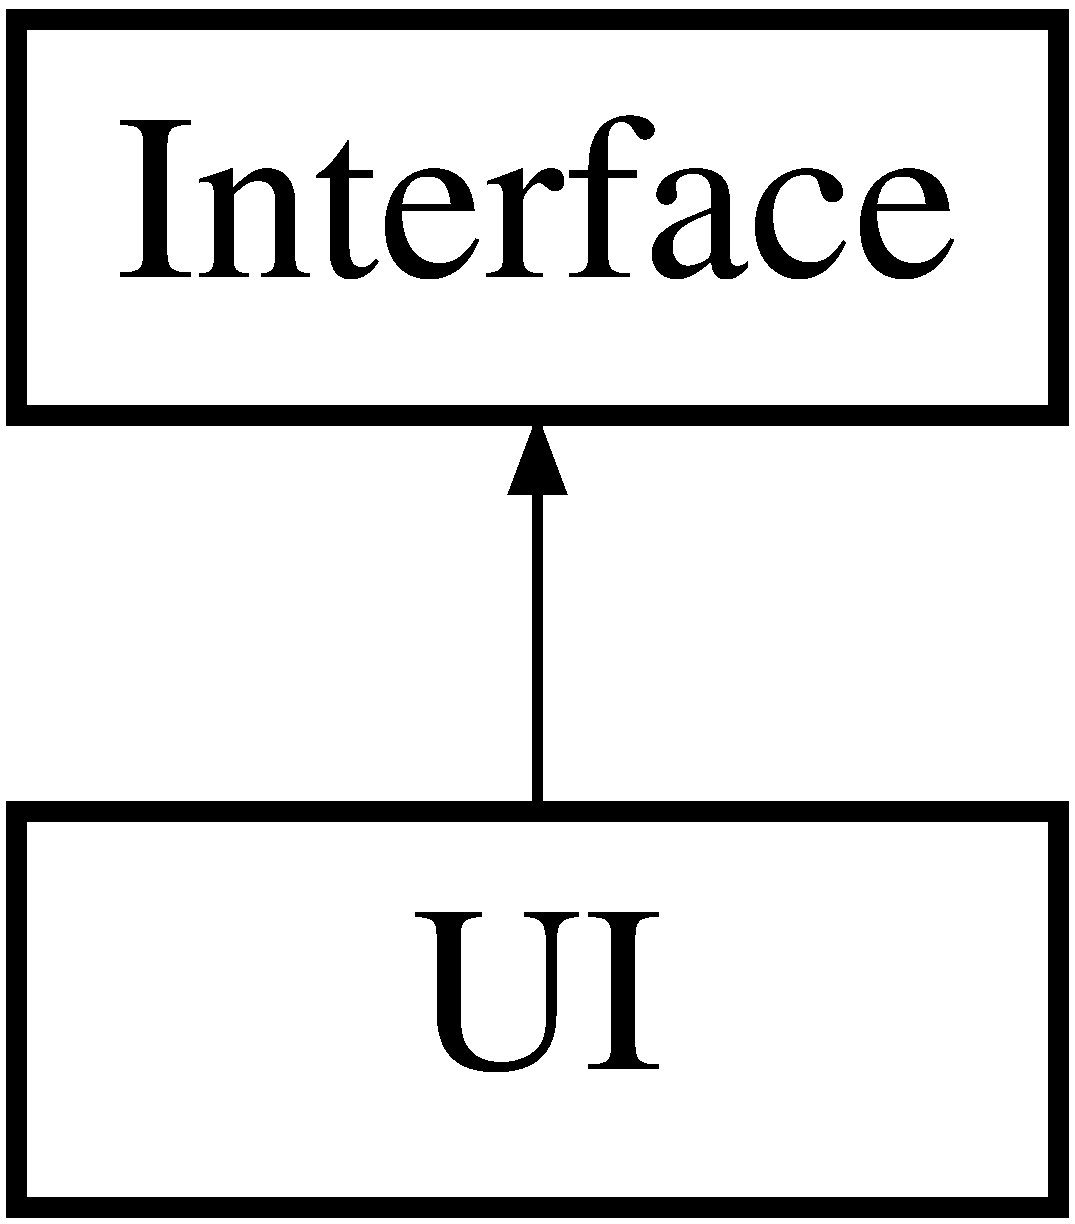
\includegraphics[height=2.000000cm]{class_u_i}
\end{center}
\end{figure}
\subsection*{Public Member Functions}
\begin{DoxyCompactItemize}
\item 
void \hyperlink{class_u_i_adb4cbcd5c39529f361c6543471e939a7}{Draw} ()
\item 
\hyperlink{class_u_i_a675985a56b5e87ebdc8e5884b9f2ee09}{U\+I} ()
\item 
virtual \hyperlink{class_u_i_a1b23d0c64c7cbb3d143d90ec532a7ccd}{$\sim$\+U\+I} ()
\end{DoxyCompactItemize}
\subsection*{Additional Inherited Members}


\subsection{Detailed Description}


Definition at line 4 of file vct\+\_\+interface.\+h.



\subsection{Constructor \& Destructor Documentation}
\hypertarget{class_u_i_a675985a56b5e87ebdc8e5884b9f2ee09}{}\index{U\+I@{U\+I}!U\+I@{U\+I}}
\index{U\+I@{U\+I}!U\+I@{U\+I}}
\subsubsection[{U\+I()}]{\setlength{\rightskip}{0pt plus 5cm}U\+I\+::\+U\+I (
\begin{DoxyParamCaption}
{}
\end{DoxyParamCaption}
)}\label{class_u_i_a675985a56b5e87ebdc8e5884b9f2ee09}


Definition at line 229 of file vct\+\_\+interface.\+cpp.

\hypertarget{class_u_i_a1b23d0c64c7cbb3d143d90ec532a7ccd}{}\index{U\+I@{U\+I}!````~U\+I@{$\sim$\+U\+I}}
\index{````~U\+I@{$\sim$\+U\+I}!U\+I@{U\+I}}
\subsubsection[{$\sim$\+U\+I()}]{\setlength{\rightskip}{0pt plus 5cm}U\+I\+::$\sim$\+U\+I (
\begin{DoxyParamCaption}
{}
\end{DoxyParamCaption}
)\hspace{0.3cm}{\ttfamily [virtual]}}\label{class_u_i_a1b23d0c64c7cbb3d143d90ec532a7ccd}


Definition at line 234 of file vct\+\_\+interface.\+cpp.



\subsection{Member Function Documentation}
\hypertarget{class_u_i_adb4cbcd5c39529f361c6543471e939a7}{}\index{U\+I@{U\+I}!Draw@{Draw}}
\index{Draw@{Draw}!U\+I@{U\+I}}
\subsubsection[{Draw()}]{\setlength{\rightskip}{0pt plus 5cm}void U\+I\+::\+Draw (
\begin{DoxyParamCaption}
{}
\end{DoxyParamCaption}
)\hspace{0.3cm}{\ttfamily [virtual]}}\label{class_u_i_adb4cbcd5c39529f361c6543471e939a7}


Implements \hyperlink{class_interface_a82df247fd022d924995421ab90444945}{Interface}.



Definition at line 7 of file vct\+\_\+interface.\+cpp.



The documentation for this class was generated from the following files\+:\begin{DoxyCompactItemize}
\item 
V\+C\+T\+\_\+\+Engine/interface/\hyperlink{vct__interface_8h}{vct\+\_\+interface.\+h}\item 
V\+C\+T\+\_\+\+Engine/interface/\hyperlink{vct__interface_8cpp}{vct\+\_\+interface.\+cpp}\end{DoxyCompactItemize}

\hypertarget{struct_vertex}{}\section{Vertex Struct Reference}
\label{struct_vertex}\index{Vertex@{Vertex}}


{\ttfamily \#include $<$vertex.\+h$>$}

\subsection*{Public Member Functions}
\begin{DoxyCompactItemize}
\item 
\hyperlink{struct_vertex_a97488994a2482d70da74e1b91d40e169}{Vertex} ()
\item 
void \hyperlink{struct_vertex_aa89fb006d01315905e0e17bdebf78757}{Orthonormalize} ()
\end{DoxyCompactItemize}
\subsection*{Public Attributes}
\begin{DoxyCompactItemize}
\item 
glm\+::vec3 \hyperlink{struct_vertex_a030819fdc241743bbd3e180a6b132ed3}{position}
\item 
glm\+::vec3 \hyperlink{struct_vertex_a825ca69622b52af1624641fbe6ecc718}{uv}
\item 
glm\+::vec3 \hyperlink{struct_vertex_a3aa35fe84025ecf1acccb5f65f5577fd}{normal}
\item 
glm\+::vec3 \hyperlink{struct_vertex_a89587fd853d4f3f42900715620a7364d}{tangent}
\item 
glm\+::vec3 \hyperlink{struct_vertex_a8c7489e0319ee0b6a214b0753907a80f}{bitangent}
\end{DoxyCompactItemize}


\subsection{Detailed Description}


Definition at line 3 of file vertex.\+h.



\subsection{Constructor \& Destructor Documentation}
\hypertarget{struct_vertex_a97488994a2482d70da74e1b91d40e169}{}\index{Vertex@{Vertex}!Vertex@{Vertex}}
\index{Vertex@{Vertex}!Vertex@{Vertex}}
\subsubsection[{Vertex()}]{\setlength{\rightskip}{0pt plus 5cm}Vertex\+::\+Vertex (
\begin{DoxyParamCaption}
{}
\end{DoxyParamCaption}
)}\label{struct_vertex_a97488994a2482d70da74e1b91d40e169}


Definition at line 4 of file vertex.\+cpp.



\subsection{Member Function Documentation}
\hypertarget{struct_vertex_aa89fb006d01315905e0e17bdebf78757}{}\index{Vertex@{Vertex}!Orthonormalize@{Orthonormalize}}
\index{Orthonormalize@{Orthonormalize}!Vertex@{Vertex}}
\subsubsection[{Orthonormalize()}]{\setlength{\rightskip}{0pt plus 5cm}void Vertex\+::\+Orthonormalize (
\begin{DoxyParamCaption}
{}
\end{DoxyParamCaption}
)}\label{struct_vertex_aa89fb006d01315905e0e17bdebf78757}


Definition at line 9 of file vertex.\+cpp.



\subsection{Member Data Documentation}
\hypertarget{struct_vertex_a8c7489e0319ee0b6a214b0753907a80f}{}\index{Vertex@{Vertex}!bitangent@{bitangent}}
\index{bitangent@{bitangent}!Vertex@{Vertex}}
\subsubsection[{bitangent}]{\setlength{\rightskip}{0pt plus 5cm}glm\+::vec3 Vertex\+::bitangent}\label{struct_vertex_a8c7489e0319ee0b6a214b0753907a80f}


Definition at line 9 of file vertex.\+h.

\hypertarget{struct_vertex_a3aa35fe84025ecf1acccb5f65f5577fd}{}\index{Vertex@{Vertex}!normal@{normal}}
\index{normal@{normal}!Vertex@{Vertex}}
\subsubsection[{normal}]{\setlength{\rightskip}{0pt plus 5cm}glm\+::vec3 Vertex\+::normal}\label{struct_vertex_a3aa35fe84025ecf1acccb5f65f5577fd}


Definition at line 7 of file vertex.\+h.

\hypertarget{struct_vertex_a030819fdc241743bbd3e180a6b132ed3}{}\index{Vertex@{Vertex}!position@{position}}
\index{position@{position}!Vertex@{Vertex}}
\subsubsection[{position}]{\setlength{\rightskip}{0pt plus 5cm}glm\+::vec3 Vertex\+::position}\label{struct_vertex_a030819fdc241743bbd3e180a6b132ed3}


Definition at line 5 of file vertex.\+h.

\hypertarget{struct_vertex_a89587fd853d4f3f42900715620a7364d}{}\index{Vertex@{Vertex}!tangent@{tangent}}
\index{tangent@{tangent}!Vertex@{Vertex}}
\subsubsection[{tangent}]{\setlength{\rightskip}{0pt plus 5cm}glm\+::vec3 Vertex\+::tangent}\label{struct_vertex_a89587fd853d4f3f42900715620a7364d}


Definition at line 8 of file vertex.\+h.

\hypertarget{struct_vertex_a825ca69622b52af1624641fbe6ecc718}{}\index{Vertex@{Vertex}!uv@{uv}}
\index{uv@{uv}!Vertex@{Vertex}}
\subsubsection[{uv}]{\setlength{\rightskip}{0pt plus 5cm}glm\+::vec3 Vertex\+::uv}\label{struct_vertex_a825ca69622b52af1624641fbe6ecc718}


Definition at line 6 of file vertex.\+h.



The documentation for this struct was generated from the following files\+:\begin{DoxyCompactItemize}
\item 
V\+C\+T\+\_\+\+Engine/types/\hyperlink{vertex_8h}{vertex.\+h}\item 
V\+C\+T\+\_\+\+Engine/types/\hyperlink{vertex_8cpp}{vertex.\+cpp}\end{DoxyCompactItemize}

\hypertarget{struct_window_settings}{}\section{Window\+Settings Struct Reference}
\label{struct_window_settings}\index{Window\+Settings@{Window\+Settings}}


{\ttfamily \#include $<$render\+\_\+window.\+h$>$}

\subsection*{Public Member Functions}
\begin{DoxyCompactItemize}
\item 
\hyperlink{struct_window_settings_a0e207ef630ccd1400f7066920b156fdf}{Window\+Settings} ()
\item 
virtual \hyperlink{struct_window_settings_a4d46e054b8672014b852f2d81ba272d3}{$\sim$\+Window\+Settings} ()
\end{DoxyCompactItemize}
\subsection*{Public Attributes}
\begin{DoxyCompactItemize}
\item 
unsigned int \hyperlink{struct_window_settings_a682fe02f872545c310d3d0dbf26720c7}{width}
\item 
unsigned int \hyperlink{struct_window_settings_a87cdc37b29add484995e2c54bcdb389b}{height}
\item 
std\+::pair$<$ int, int $>$ \hyperlink{struct_window_settings_a041200534ceac3296a8eb4b0dd1bbe30}{position}
\item 
std\+::string \hyperlink{struct_window_settings_a5f56c222507f096ac106b06235ac53e8}{title}
\end{DoxyCompactItemize}


\subsection{Detailed Description}


Definition at line 2 of file render\+\_\+window.\+h.



\subsection{Constructor \& Destructor Documentation}
\hypertarget{struct_window_settings_a0e207ef630ccd1400f7066920b156fdf}{}\index{Window\+Settings@{Window\+Settings}!Window\+Settings@{Window\+Settings}}
\index{Window\+Settings@{Window\+Settings}!Window\+Settings@{Window\+Settings}}
\subsubsection[{Window\+Settings()}]{\setlength{\rightskip}{0pt plus 5cm}Window\+Settings\+::\+Window\+Settings (
\begin{DoxyParamCaption}
{}
\end{DoxyParamCaption}
)\hspace{0.3cm}{\ttfamily [inline]}}\label{struct_window_settings_a0e207ef630ccd1400f7066920b156fdf}


Definition at line 8 of file render\+\_\+window.\+h.

\hypertarget{struct_window_settings_a4d46e054b8672014b852f2d81ba272d3}{}\index{Window\+Settings@{Window\+Settings}!````~Window\+Settings@{$\sim$\+Window\+Settings}}
\index{````~Window\+Settings@{$\sim$\+Window\+Settings}!Window\+Settings@{Window\+Settings}}
\subsubsection[{$\sim$\+Window\+Settings()}]{\setlength{\rightskip}{0pt plus 5cm}virtual Window\+Settings\+::$\sim$\+Window\+Settings (
\begin{DoxyParamCaption}
{}
\end{DoxyParamCaption}
)\hspace{0.3cm}{\ttfamily [inline]}, {\ttfamily [virtual]}}\label{struct_window_settings_a4d46e054b8672014b852f2d81ba272d3}


Definition at line 9 of file render\+\_\+window.\+h.



\subsection{Member Data Documentation}
\hypertarget{struct_window_settings_a87cdc37b29add484995e2c54bcdb389b}{}\index{Window\+Settings@{Window\+Settings}!height@{height}}
\index{height@{height}!Window\+Settings@{Window\+Settings}}
\subsubsection[{height}]{\setlength{\rightskip}{0pt plus 5cm}unsigned int Window\+Settings\+::height}\label{struct_window_settings_a87cdc37b29add484995e2c54bcdb389b}


Definition at line 5 of file render\+\_\+window.\+h.

\hypertarget{struct_window_settings_a041200534ceac3296a8eb4b0dd1bbe30}{}\index{Window\+Settings@{Window\+Settings}!position@{position}}
\index{position@{position}!Window\+Settings@{Window\+Settings}}
\subsubsection[{position}]{\setlength{\rightskip}{0pt plus 5cm}std\+::pair$<$int, int$>$ Window\+Settings\+::position}\label{struct_window_settings_a041200534ceac3296a8eb4b0dd1bbe30}


Definition at line 6 of file render\+\_\+window.\+h.

\hypertarget{struct_window_settings_a5f56c222507f096ac106b06235ac53e8}{}\index{Window\+Settings@{Window\+Settings}!title@{title}}
\index{title@{title}!Window\+Settings@{Window\+Settings}}
\subsubsection[{title}]{\setlength{\rightskip}{0pt plus 5cm}std\+::string Window\+Settings\+::title}\label{struct_window_settings_a5f56c222507f096ac106b06235ac53e8}


Definition at line 7 of file render\+\_\+window.\+h.

\hypertarget{struct_window_settings_a682fe02f872545c310d3d0dbf26720c7}{}\index{Window\+Settings@{Window\+Settings}!width@{width}}
\index{width@{width}!Window\+Settings@{Window\+Settings}}
\subsubsection[{width}]{\setlength{\rightskip}{0pt plus 5cm}unsigned int Window\+Settings\+::width}\label{struct_window_settings_a682fe02f872545c310d3d0dbf26720c7}


Definition at line 4 of file render\+\_\+window.\+h.



The documentation for this struct was generated from the following file\+:\begin{DoxyCompactItemize}
\item 
V\+C\+T\+\_\+\+Engine/interface/\hyperlink{render__window_8h}{render\+\_\+window.\+h}\end{DoxyCompactItemize}

\chapter{File Documentation}
\hypertarget{deferred__handler_8cpp}{}\section{V\+C\+T\+\_\+\+Engine/core/deferred\+\_\+handler.cpp File Reference}
\label{deferred__handler_8cpp}\index{V\+C\+T\+\_\+\+Engine/core/deferred\+\_\+handler.\+cpp@{V\+C\+T\+\_\+\+Engine/core/deferred\+\_\+handler.\+cpp}}
{\ttfamily \#include \char`\"{}stdafx.\+h\char`\"{}}\\*
{\ttfamily \#include \char`\"{}deferred\+\_\+handler.\+h\char`\"{}}\\*
{\ttfamily \#include \char`\"{}scene\textbackslash{}light.\+h\char`\"{}}\\*

\hypertarget{deferred__handler_8h}{}\section{V\+C\+T\+\_\+\+Engine/core/deferred\+\_\+handler.h File Reference}
\label{deferred__handler_8h}\index{V\+C\+T\+\_\+\+Engine/core/deferred\+\_\+handler.\+h@{V\+C\+T\+\_\+\+Engine/core/deferred\+\_\+handler.\+h}}
{\ttfamily \#include \char`\"{}scene\textbackslash{}texture.\+h\char`\"{}}\\*
{\ttfamily \#include \char`\"{}types\textbackslash{}transform\+\_\+matrices.\+h\char`\"{}}\\*
{\ttfamily \#include \char`\"{}scene\textbackslash{}material.\+h\char`\"{}}\\*
{\ttfamily \#include \char`\"{}scene\textbackslash{}light.\+h\char`\"{}}\\*
\subsection*{Classes}
\begin{DoxyCompactItemize}
\item 
class \hyperlink{class_deferred_program}{Deferred\+Program}
\item 
struct \hyperlink{struct_deferred_program_1_1_light_uniform_1_1_attenuation_uniform}{Deferred\+Program\+::\+Light\+Uniform\+::\+Attenuation\+Uniform}
\item 
class \hyperlink{class_deferred_handler}{Deferred\+Handler}
\end{DoxyCompactItemize}
\subsection*{Enumerations}
\begin{DoxyCompactItemize}
\item 
enum \hyperlink{deferred__handler_8h_a331a939e08dff83e0b0b62fbbd39c963}{G\+Buffer\+Texture\+Id} \+: unsigned int \{ \\*
\hyperlink{deferred__handler_8h_a331a939e08dff83e0b0b62fbbd39c963a52f5e0bc3859bc5f5e25130b6c7e8881}{G\+Buffer\+Texture\+Id\+::\+Position}, 
\hyperlink{deferred__handler_8h_a331a939e08dff83e0b0b62fbbd39c963a960b44c579bc2f6818d2daaf9e4c16f0}{G\+Buffer\+Texture\+Id\+::\+Normal}, 
\hyperlink{deferred__handler_8h_a331a939e08dff83e0b0b62fbbd39c963af879d0a27915d351a8e47c2223777710}{G\+Buffer\+Texture\+Id\+::\+Albedo}, 
\hyperlink{deferred__handler_8h_a331a939e08dff83e0b0b62fbbd39c963a39b0044dd8789d333e7794f359406740}{G\+Buffer\+Texture\+Id\+::\+Specular}, 
\\*
\hyperlink{deferred__handler_8h_a331a939e08dff83e0b0b62fbbd39c963aab6a10807f81dc6cf6b5a7db474c163e}{G\+Buffer\+Texture\+Id\+::\+G\+B\+U\+F\+F\+E\+R\+\_\+\+T\+E\+X\+T\+U\+R\+E\+\_\+\+T\+Y\+P\+E\+\_\+\+M\+A\+X}
 \}
\item 
enum \hyperlink{deferred__handler_8h_a623ca9c5815b447740795ef10bc3a9fe}{Deferred\+Stage} \+: unsigned int \{ \hyperlink{deferred__handler_8h_a623ca9c5815b447740795ef10bc3a9fead9c6333623e6357515fcbf17be806273}{Deferred\+Stage\+::\+Geometry}, 
\hyperlink{deferred__handler_8h_a623ca9c5815b447740795ef10bc3a9fea2e4b97fde8cf63085ec969fcc7e490c0}{Deferred\+Stage\+::\+Lighting}
 \}
\end{DoxyCompactItemize}


\subsection{Enumeration Type Documentation}
\hypertarget{deferred__handler_8h_a623ca9c5815b447740795ef10bc3a9fe}{}\index{deferred\+\_\+handler.\+h@{deferred\+\_\+handler.\+h}!Deferred\+Stage@{Deferred\+Stage}}
\index{Deferred\+Stage@{Deferred\+Stage}!deferred\+\_\+handler.\+h@{deferred\+\_\+handler.\+h}}
\subsubsection[{Deferred\+Stage}]{\setlength{\rightskip}{0pt plus 5cm}enum {\bf Deferred\+Stage} \+: unsigned int\hspace{0.3cm}{\ttfamily [strong]}}\label{deferred__handler_8h_a623ca9c5815b447740795ef10bc3a9fe}
\begin{Desc}
\item[Enumerator]\par
\begin{description}
\index{Geometry@{Geometry}!deferred\+\_\+handler.\+h@{deferred\+\_\+handler.\+h}}\index{deferred\+\_\+handler.\+h@{deferred\+\_\+handler.\+h}!Geometry@{Geometry}}\item[{\em 
\hypertarget{deferred__handler_8h_a623ca9c5815b447740795ef10bc3a9fead9c6333623e6357515fcbf17be806273}{}Geometry\label{deferred__handler_8h_a623ca9c5815b447740795ef10bc3a9fead9c6333623e6357515fcbf17be806273}
}]\index{Lighting@{Lighting}!deferred\+\_\+handler.\+h@{deferred\+\_\+handler.\+h}}\index{deferred\+\_\+handler.\+h@{deferred\+\_\+handler.\+h}!Lighting@{Lighting}}\item[{\em 
\hypertarget{deferred__handler_8h_a623ca9c5815b447740795ef10bc3a9fea2e4b97fde8cf63085ec969fcc7e490c0}{}Lighting\label{deferred__handler_8h_a623ca9c5815b447740795ef10bc3a9fea2e4b97fde8cf63085ec969fcc7e490c0}
}]\end{description}
\end{Desc}


Definition at line 16 of file deferred\+\_\+handler.\+h.

\hypertarget{deferred__handler_8h_a331a939e08dff83e0b0b62fbbd39c963}{}\index{deferred\+\_\+handler.\+h@{deferred\+\_\+handler.\+h}!G\+Buffer\+Texture\+Id@{G\+Buffer\+Texture\+Id}}
\index{G\+Buffer\+Texture\+Id@{G\+Buffer\+Texture\+Id}!deferred\+\_\+handler.\+h@{deferred\+\_\+handler.\+h}}
\subsubsection[{G\+Buffer\+Texture\+Id}]{\setlength{\rightskip}{0pt plus 5cm}enum {\bf G\+Buffer\+Texture\+Id} \+: unsigned int\hspace{0.3cm}{\ttfamily [strong]}}\label{deferred__handler_8h_a331a939e08dff83e0b0b62fbbd39c963}
\begin{Desc}
\item[Enumerator]\par
\begin{description}
\index{Position@{Position}!deferred\+\_\+handler.\+h@{deferred\+\_\+handler.\+h}}\index{deferred\+\_\+handler.\+h@{deferred\+\_\+handler.\+h}!Position@{Position}}\item[{\em 
\hypertarget{deferred__handler_8h_a331a939e08dff83e0b0b62fbbd39c963a52f5e0bc3859bc5f5e25130b6c7e8881}{}Position\label{deferred__handler_8h_a331a939e08dff83e0b0b62fbbd39c963a52f5e0bc3859bc5f5e25130b6c7e8881}
}]\index{Normal@{Normal}!deferred\+\_\+handler.\+h@{deferred\+\_\+handler.\+h}}\index{deferred\+\_\+handler.\+h@{deferred\+\_\+handler.\+h}!Normal@{Normal}}\item[{\em 
\hypertarget{deferred__handler_8h_a331a939e08dff83e0b0b62fbbd39c963a960b44c579bc2f6818d2daaf9e4c16f0}{}Normal\label{deferred__handler_8h_a331a939e08dff83e0b0b62fbbd39c963a960b44c579bc2f6818d2daaf9e4c16f0}
}]\index{Albedo@{Albedo}!deferred\+\_\+handler.\+h@{deferred\+\_\+handler.\+h}}\index{deferred\+\_\+handler.\+h@{deferred\+\_\+handler.\+h}!Albedo@{Albedo}}\item[{\em 
\hypertarget{deferred__handler_8h_a331a939e08dff83e0b0b62fbbd39c963af879d0a27915d351a8e47c2223777710}{}Albedo\label{deferred__handler_8h_a331a939e08dff83e0b0b62fbbd39c963af879d0a27915d351a8e47c2223777710}
}]\index{Specular@{Specular}!deferred\+\_\+handler.\+h@{deferred\+\_\+handler.\+h}}\index{deferred\+\_\+handler.\+h@{deferred\+\_\+handler.\+h}!Specular@{Specular}}\item[{\em 
\hypertarget{deferred__handler_8h_a331a939e08dff83e0b0b62fbbd39c963a39b0044dd8789d333e7794f359406740}{}Specular\label{deferred__handler_8h_a331a939e08dff83e0b0b62fbbd39c963a39b0044dd8789d333e7794f359406740}
}]\index{G\+B\+U\+F\+F\+E\+R\+\_\+\+T\+E\+X\+T\+U\+R\+E\+\_\+\+T\+Y\+P\+E\+\_\+\+M\+A\+X@{G\+B\+U\+F\+F\+E\+R\+\_\+\+T\+E\+X\+T\+U\+R\+E\+\_\+\+T\+Y\+P\+E\+\_\+\+M\+A\+X}!deferred\+\_\+handler.\+h@{deferred\+\_\+handler.\+h}}\index{deferred\+\_\+handler.\+h@{deferred\+\_\+handler.\+h}!G\+B\+U\+F\+F\+E\+R\+\_\+\+T\+E\+X\+T\+U\+R\+E\+\_\+\+T\+Y\+P\+E\+\_\+\+M\+A\+X@{G\+B\+U\+F\+F\+E\+R\+\_\+\+T\+E\+X\+T\+U\+R\+E\+\_\+\+T\+Y\+P\+E\+\_\+\+M\+A\+X}}\item[{\em 
\hypertarget{deferred__handler_8h_a331a939e08dff83e0b0b62fbbd39c963aab6a10807f81dc6cf6b5a7db474c163e}{}G\+B\+U\+F\+F\+E\+R\+\_\+\+T\+E\+X\+T\+U\+R\+E\+\_\+\+T\+Y\+P\+E\+\_\+\+M\+A\+X\label{deferred__handler_8h_a331a939e08dff83e0b0b62fbbd39c963aab6a10807f81dc6cf6b5a7db474c163e}
}]\end{description}
\end{Desc}


Definition at line 7 of file deferred\+\_\+handler.\+h.


\hypertarget{engine__assets_8cpp}{}\section{V\+C\+T\+\_\+\+Engine/core/engine\+\_\+assets.cpp File Reference}
\label{engine__assets_8cpp}\index{V\+C\+T\+\_\+\+Engine/core/engine\+\_\+assets.\+cpp@{V\+C\+T\+\_\+\+Engine/core/engine\+\_\+assets.\+cpp}}
{\ttfamily \#include \char`\"{}stdafx.\+h\char`\"{}}\\*
{\ttfamily \#include \char`\"{}engine\+\_\+assets.\+h\char`\"{}}\\*
{\ttfamily \#include \char`\"{}engine\+\_\+base.\+h\char`\"{}}\\*

\hypertarget{engine__assets_8h}{}\section{V\+C\+T\+\_\+\+Engine/core/engine\+\_\+assets.h File Reference}
\label{engine__assets_8h}\index{V\+C\+T\+\_\+\+Engine/core/engine\+\_\+assets.\+h@{V\+C\+T\+\_\+\+Engine/core/engine\+\_\+assets.\+h}}
{\ttfamily \#include \char`\"{}util\textbackslash{}scene\+\_\+importer.\+h\char`\"{}}\\*
\subsection*{Classes}
\begin{DoxyCompactItemize}
\item 
class \hyperlink{class_engine_assets}{Engine\+Assets}
\end{DoxyCompactItemize}

\hypertarget{engine__base_8cpp}{}\section{V\+C\+T\+\_\+\+Engine/core/engine\+\_\+base.cpp File Reference}
\label{engine__base_8cpp}\index{V\+C\+T\+\_\+\+Engine/core/engine\+\_\+base.\+cpp@{V\+C\+T\+\_\+\+Engine/core/engine\+\_\+base.\+cpp}}
{\ttfamily \#include \char`\"{}stdafx.\+h\char`\"{}}\\*
{\ttfamily \#include \char`\"{}engine\+\_\+base.\+h\char`\"{}}\\*
{\ttfamily \#include \char`\"{}scene\textbackslash{}camera.\+h\char`\"{}}\\*

\hypertarget{engine__base_8h}{}\section{V\+C\+T\+\_\+\+Engine/core/engine\+\_\+base.h File Reference}
\label{engine__base_8h}\index{V\+C\+T\+\_\+\+Engine/core/engine\+\_\+base.\+h@{V\+C\+T\+\_\+\+Engine/core/engine\+\_\+base.\+h}}
{\ttfamily \#include \char`\"{}interface\textbackslash{}render\+\_\+window.\+h\char`\"{}}\\*
{\ttfamily \#include \char`\"{}misc\textbackslash{}\+External\+\_\+initializer.\+h\char`\"{}}\\*
{\ttfamily \#include \char`\"{}interface\textbackslash{}vct\+\_\+interface.\+h\char`\"{}}\\*
{\ttfamily \#include \char`\"{}engine\+\_\+assets.\+h\char`\"{}}\\*
{\ttfamily \#include \char`\"{}deferred\+\_\+handler.\+h\char`\"{}}\\*
{\ttfamily \#include \char`\"{}renderer.\+h\char`\"{}}\\*
\subsection*{Classes}
\begin{DoxyCompactItemize}
\item 
class \hyperlink{class_execution_info}{Execution\+Info}
\item 
class \hyperlink{class_engine_base}{Engine\+Base}
\end{DoxyCompactItemize}

\hypertarget{renderer_8cpp}{}\section{V\+C\+T\+\_\+\+Engine/core/renderer.cpp File Reference}
\label{renderer_8cpp}\index{V\+C\+T\+\_\+\+Engine/core/renderer.\+cpp@{V\+C\+T\+\_\+\+Engine/core/renderer.\+cpp}}
{\ttfamily \#include \char`\"{}stdafx.\+h\char`\"{}}\\*
{\ttfamily \#include \char`\"{}renderer.\+h\char`\"{}}\\*
{\ttfamily \#include \char`\"{}engine\+\_\+base.\+h\char`\"{}}\\*

\hypertarget{renderer_8h}{}\section{V\+C\+T\+\_\+\+Engine/core/renderer.h File Reference}
\label{renderer_8h}\index{V\+C\+T\+\_\+\+Engine/core/renderer.\+h@{V\+C\+T\+\_\+\+Engine/core/renderer.\+h}}
{\ttfamily \#include \char`\"{}scene\textbackslash{}scene.\+h\char`\"{}}\\*
{\ttfamily \#include \char`\"{}deferred\+\_\+handler.\+h\char`\"{}}\\*
{\ttfamily \#include \char`\"{}interface\textbackslash{}render\+\_\+window.\+h\char`\"{}}\\*
{\ttfamily \#include \char`\"{}types\textbackslash{}transform\+\_\+matrices.\+h\char`\"{}}\\*
{\ttfamily \#include \char`\"{}types\textbackslash{}frustum.\+h\char`\"{}}\\*
\subsection*{Classes}
\begin{DoxyCompactItemize}
\item 
class \hyperlink{class_renderer}{Renderer}
\end{DoxyCompactItemize}

\hypertarget{interface_8cpp}{}\section{V\+C\+T\+\_\+\+Engine/interface/interface.cpp File Reference}
\label{interface_8cpp}\index{V\+C\+T\+\_\+\+Engine/interface/interface.\+cpp@{V\+C\+T\+\_\+\+Engine/interface/interface.\+cpp}}
{\ttfamily \#include \char`\"{}stdafx.\+h\char`\"{}}\\*
{\ttfamily \#include \char`\"{}interface.\+h\char`\"{}}\\*
\subsection*{Macros}
\begin{DoxyCompactItemize}
\item 
\#define \hyperlink{interface_8cpp_aaa4726ae33d556805a771475548e5671}{O\+F\+F\+S\+E\+T\+O\+F}(T\+Y\+P\+E,  E\+L\+E\+M\+E\+N\+T)~((size\+\_\+t)\&(((T\+Y\+P\+E $\ast$)0)-\/$>$E\+L\+E\+M\+E\+N\+T))
\end{DoxyCompactItemize}


\subsection{Macro Definition Documentation}
\hypertarget{interface_8cpp_aaa4726ae33d556805a771475548e5671}{}\index{interface.\+cpp@{interface.\+cpp}!O\+F\+F\+S\+E\+T\+O\+F@{O\+F\+F\+S\+E\+T\+O\+F}}
\index{O\+F\+F\+S\+E\+T\+O\+F@{O\+F\+F\+S\+E\+T\+O\+F}!interface.\+cpp@{interface.\+cpp}}
\subsubsection[{O\+F\+F\+S\+E\+T\+O\+F}]{\setlength{\rightskip}{0pt plus 5cm}\#define O\+F\+F\+S\+E\+T\+O\+F(
\begin{DoxyParamCaption}
\item[{}]{T\+Y\+P\+E, }
\item[{}]{E\+L\+E\+M\+E\+N\+T}
\end{DoxyParamCaption}
)~((size\+\_\+t)\&(((T\+Y\+P\+E $\ast$)0)-\/$>$E\+L\+E\+M\+E\+N\+T))}\label{interface_8cpp_aaa4726ae33d556805a771475548e5671}

\hypertarget{interface_8h}{}\section{V\+C\+T\+\_\+\+Engine/interface/interface.h File Reference}
\label{interface_8h}\index{V\+C\+T\+\_\+\+Engine/interface/interface.\+h@{V\+C\+T\+\_\+\+Engine/interface/interface.\+h}}
{\ttfamily \#include \char`\"{}render\+\_\+window.\+h\char`\"{}}\\*
\subsection*{Classes}
\begin{DoxyCompactItemize}
\item 
class \hyperlink{class_interface}{Interface}
\end{DoxyCompactItemize}

\hypertarget{render__window_8cpp}{}\section{V\+C\+T\+\_\+\+Engine/interface/render\+\_\+window.cpp File Reference}
\label{render__window_8cpp}\index{V\+C\+T\+\_\+\+Engine/interface/render\+\_\+window.\+cpp@{V\+C\+T\+\_\+\+Engine/interface/render\+\_\+window.\+cpp}}
{\ttfamily \#include \char`\"{}stdafx.\+h\char`\"{}}\\*
{\ttfamily \#include \char`\"{}render\+\_\+window.\+h\char`\"{}}\\*

\hypertarget{render__window_8h}{}\section{V\+C\+T\+\_\+\+Engine/interface/render\+\_\+window.h File Reference}
\label{render__window_8h}\index{V\+C\+T\+\_\+\+Engine/interface/render\+\_\+window.\+h@{V\+C\+T\+\_\+\+Engine/interface/render\+\_\+window.\+h}}
\subsection*{Classes}
\begin{DoxyCompactItemize}
\item 
struct \hyperlink{struct_window_settings}{Window\+Settings}
\item 
class \hyperlink{class_render_window}{Render\+Window}
\end{DoxyCompactItemize}

\hypertarget{vct__interface_8cpp}{}\section{V\+C\+T\+\_\+\+Engine/interface/vct\+\_\+interface.cpp File Reference}
\label{vct__interface_8cpp}\index{V\+C\+T\+\_\+\+Engine/interface/vct\+\_\+interface.\+cpp@{V\+C\+T\+\_\+\+Engine/interface/vct\+\_\+interface.\+cpp}}
{\ttfamily \#include \char`\"{}stdafx.\+h\char`\"{}}\\*
{\ttfamily \#include \char`\"{}vct\+\_\+interface.\+h\char`\"{}}\\*
{\ttfamily \#include \char`\"{}core\textbackslash{}engine\+\_\+base.\+h\char`\"{}}\\*
{\ttfamily \#include \char`\"{}core\textbackslash{}deferred\+\_\+handler.\+h\char`\"{}}\\*

\hypertarget{vct__interface_8h}{}\section{V\+C\+T\+\_\+\+Engine/interface/vct\+\_\+interface.h File Reference}
\label{vct__interface_8h}\index{V\+C\+T\+\_\+\+Engine/interface/vct\+\_\+interface.\+h@{V\+C\+T\+\_\+\+Engine/interface/vct\+\_\+interface.\+h}}
{\ttfamily \#include \char`\"{}interface.\+h\char`\"{}}\\*
\subsection*{Classes}
\begin{DoxyCompactItemize}
\item 
class \hyperlink{class_u_i}{U\+I}
\end{DoxyCompactItemize}

\hypertarget{main_8cpp}{}\section{V\+C\+T\+\_\+\+Engine/main.cpp File Reference}
\label{main_8cpp}\index{V\+C\+T\+\_\+\+Engine/main.\+cpp@{V\+C\+T\+\_\+\+Engine/main.\+cpp}}
{\ttfamily \#include \char`\"{}stdafx.\+h\char`\"{}}\\*
{\ttfamily \#include \char`\"{}core\textbackslash{}engine\+\_\+base.\+h\char`\"{}}\\*
\subsection*{Functions}
\begin{DoxyCompactItemize}
\item 
int \hyperlink{main_8cpp_a0ddf1224851353fc92bfbff6f499fa97}{main} (int argc, char $\ast$argv\mbox{[}$\,$\mbox{]})
\end{DoxyCompactItemize}


\subsection{Function Documentation}
\hypertarget{main_8cpp_a0ddf1224851353fc92bfbff6f499fa97}{}\index{main.\+cpp@{main.\+cpp}!main@{main}}
\index{main@{main}!main.\+cpp@{main.\+cpp}}
\subsubsection[{main(int argc, char $\ast$argv[])}]{\setlength{\rightskip}{0pt plus 5cm}int main (
\begin{DoxyParamCaption}
\item[{int}]{argc, }
\item[{char $\ast$}]{argv\mbox{[}$\,$\mbox{]}}
\end{DoxyParamCaption}
)}\label{main_8cpp_a0ddf1224851353fc92bfbff6f499fa97}


Definition at line 9 of file main.\+cpp.


\hypertarget{external__initializer_8cpp}{}\section{V\+C\+T\+\_\+\+Engine/misc/external\+\_\+initializer.cpp File Reference}
\label{external__initializer_8cpp}\index{V\+C\+T\+\_\+\+Engine/misc/external\+\_\+initializer.\+cpp@{V\+C\+T\+\_\+\+Engine/misc/external\+\_\+initializer.\+cpp}}
{\ttfamily \#include \char`\"{}stdafx.\+h\char`\"{}}\\*
{\ttfamily \#include \char`\"{}external\+\_\+initializer.\+h\char`\"{}}\\*
{\ttfamily \#include \char`\"{}Free\+Image.\+h\char`\"{}}\\*
{\ttfamily \#include \char`\"{}assimp\textbackslash{}\+Importer.\+hpp\char`\"{}}\\*
{\ttfamily \#include \char`\"{}assimp\textbackslash{}version.\+h\char`\"{}}\\*

\hypertarget{external__initializer_8h}{}\section{V\+C\+T\+\_\+\+Engine/misc/external\+\_\+initializer.h File Reference}
\label{external__initializer_8h}\index{V\+C\+T\+\_\+\+Engine/misc/external\+\_\+initializer.\+h@{V\+C\+T\+\_\+\+Engine/misc/external\+\_\+initializer.\+h}}
\subsection*{Classes}
\begin{DoxyCompactItemize}
\item 
class \hyperlink{class_external_initializer}{External\+Initializer}
\end{DoxyCompactItemize}

\hypertarget{miscellaneous_8cpp}{}\section{V\+C\+T\+\_\+\+Engine/misc/miscellaneous.cpp File Reference}
\label{miscellaneous_8cpp}\index{V\+C\+T\+\_\+\+Engine/misc/miscellaneous.\+cpp@{V\+C\+T\+\_\+\+Engine/misc/miscellaneous.\+cpp}}
{\ttfamily \#include \char`\"{}stdafx.\+h\char`\"{}}\\*
\subsection*{Functions}
\begin{DoxyCompactItemize}
\item 
void \hyperlink{miscellaneous_8cpp_a0098ba6d57d95194a574af7f28b16ea0}{Console\+Progress\+Bar} (const std\+::string \&title, int bar\+Width, int index, int last)
\item 
std\+::string \hyperlink{miscellaneous_8cpp_af252ff1df365d9c524663defcf1a4425}{Get\+Directory\+Path} (const std\+::string \&file\+Path)
\item 
void \hyperlink{miscellaneous_8cpp_aa8a8eebb4e7d2754fa2a7df4b872314c}{Skip\+B\+O\+M} (std\+::ifstream \&in)
\end{DoxyCompactItemize}


\subsection{Function Documentation}
\hypertarget{miscellaneous_8cpp_a0098ba6d57d95194a574af7f28b16ea0}{}\index{miscellaneous.\+cpp@{miscellaneous.\+cpp}!Console\+Progress\+Bar@{Console\+Progress\+Bar}}
\index{Console\+Progress\+Bar@{Console\+Progress\+Bar}!miscellaneous.\+cpp@{miscellaneous.\+cpp}}
\subsubsection[{Console\+Progress\+Bar(const std\+::string \&title, int bar\+Width, int index, int last)}]{\setlength{\rightskip}{0pt plus 5cm}void Console\+Progress\+Bar (
\begin{DoxyParamCaption}
\item[{const std\+::string \&}]{title, }
\item[{int}]{bar\+Width, }
\item[{int}]{index, }
\item[{int}]{last}
\end{DoxyParamCaption}
)}\label{miscellaneous_8cpp_a0098ba6d57d95194a574af7f28b16ea0}


Definition at line 3 of file miscellaneous.\+cpp.

\hypertarget{miscellaneous_8cpp_af252ff1df365d9c524663defcf1a4425}{}\index{miscellaneous.\+cpp@{miscellaneous.\+cpp}!Get\+Directory\+Path@{Get\+Directory\+Path}}
\index{Get\+Directory\+Path@{Get\+Directory\+Path}!miscellaneous.\+cpp@{miscellaneous.\+cpp}}
\subsubsection[{Get\+Directory\+Path(const std\+::string \&file\+Path)}]{\setlength{\rightskip}{0pt plus 5cm}std\+::string Get\+Directory\+Path (
\begin{DoxyParamCaption}
\item[{const std\+::string \&}]{file\+Path}
\end{DoxyParamCaption}
)}\label{miscellaneous_8cpp_af252ff1df365d9c524663defcf1a4425}


Definition at line 21 of file miscellaneous.\+cpp.

\hypertarget{miscellaneous_8cpp_aa8a8eebb4e7d2754fa2a7df4b872314c}{}\index{miscellaneous.\+cpp@{miscellaneous.\+cpp}!Skip\+B\+O\+M@{Skip\+B\+O\+M}}
\index{Skip\+B\+O\+M@{Skip\+B\+O\+M}!miscellaneous.\+cpp@{miscellaneous.\+cpp}}
\subsubsection[{Skip\+B\+O\+M(std\+::ifstream \&in)}]{\setlength{\rightskip}{0pt plus 5cm}void Skip\+B\+O\+M (
\begin{DoxyParamCaption}
\item[{std\+::ifstream \&}]{in}
\end{DoxyParamCaption}
)}\label{miscellaneous_8cpp_aa8a8eebb4e7d2754fa2a7df4b872314c}


Definition at line 27 of file miscellaneous.\+cpp.


\hypertarget{miscellaneous_8h}{}\section{V\+C\+T\+\_\+\+Engine/misc/miscellaneous.h File Reference}
\label{miscellaneous_8h}\index{V\+C\+T\+\_\+\+Engine/misc/miscellaneous.\+h@{V\+C\+T\+\_\+\+Engine/misc/miscellaneous.\+h}}
\subsection*{Functions}
\begin{DoxyCompactItemize}
\item 
void \hyperlink{miscellaneous_8h_a0098ba6d57d95194a574af7f28b16ea0}{Console\+Progress\+Bar} (const std\+::string \&title, int bar\+Width, int index, int last)
\item 
void \hyperlink{miscellaneous_8h_aa8a8eebb4e7d2754fa2a7df4b872314c}{Skip\+B\+O\+M} (std\+::ifstream \&in)
\item 
std\+::string \hyperlink{miscellaneous_8h_af252ff1df365d9c524663defcf1a4425}{Get\+Directory\+Path} (const std\+::string \&file\+Path)
\end{DoxyCompactItemize}


\subsection{Function Documentation}
\hypertarget{miscellaneous_8h_a0098ba6d57d95194a574af7f28b16ea0}{}\index{miscellaneous.\+h@{miscellaneous.\+h}!Console\+Progress\+Bar@{Console\+Progress\+Bar}}
\index{Console\+Progress\+Bar@{Console\+Progress\+Bar}!miscellaneous.\+h@{miscellaneous.\+h}}
\subsubsection[{Console\+Progress\+Bar(const std\+::string \&title, int bar\+Width, int index, int last)}]{\setlength{\rightskip}{0pt plus 5cm}void Console\+Progress\+Bar (
\begin{DoxyParamCaption}
\item[{const std\+::string \&}]{title, }
\item[{int}]{bar\+Width, }
\item[{int}]{index, }
\item[{int}]{last}
\end{DoxyParamCaption}
)}\label{miscellaneous_8h_a0098ba6d57d95194a574af7f28b16ea0}


Definition at line 3 of file miscellaneous.\+cpp.

\hypertarget{miscellaneous_8h_af252ff1df365d9c524663defcf1a4425}{}\index{miscellaneous.\+h@{miscellaneous.\+h}!Get\+Directory\+Path@{Get\+Directory\+Path}}
\index{Get\+Directory\+Path@{Get\+Directory\+Path}!miscellaneous.\+h@{miscellaneous.\+h}}
\subsubsection[{Get\+Directory\+Path(const std\+::string \&file\+Path)}]{\setlength{\rightskip}{0pt plus 5cm}std\+::string Get\+Directory\+Path (
\begin{DoxyParamCaption}
\item[{const std\+::string \&}]{file\+Path}
\end{DoxyParamCaption}
)}\label{miscellaneous_8h_af252ff1df365d9c524663defcf1a4425}


Definition at line 21 of file miscellaneous.\+cpp.

\hypertarget{miscellaneous_8h_aa8a8eebb4e7d2754fa2a7df4b872314c}{}\index{miscellaneous.\+h@{miscellaneous.\+h}!Skip\+B\+O\+M@{Skip\+B\+O\+M}}
\index{Skip\+B\+O\+M@{Skip\+B\+O\+M}!miscellaneous.\+h@{miscellaneous.\+h}}
\subsubsection[{Skip\+B\+O\+M(std\+::ifstream \&in)}]{\setlength{\rightskip}{0pt plus 5cm}void Skip\+B\+O\+M (
\begin{DoxyParamCaption}
\item[{std\+::ifstream \&}]{in}
\end{DoxyParamCaption}
)}\label{miscellaneous_8h_aa8a8eebb4e7d2754fa2a7df4b872314c}


Definition at line 27 of file miscellaneous.\+cpp.


\hypertarget{camera_8cpp}{}\section{V\+C\+T\+\_\+\+Engine/scene/camera.cpp File Reference}
\label{camera_8cpp}\index{V\+C\+T\+\_\+\+Engine/scene/camera.\+cpp@{V\+C\+T\+\_\+\+Engine/scene/camera.\+cpp}}
{\ttfamily \#include \char`\"{}stdafx.\+h\char`\"{}}\\*
{\ttfamily \#include \char`\"{}camera.\+h\char`\"{}}\\*

\hypertarget{camera_8h}{}\section{V\+C\+T\+\_\+\+Engine/scene/camera.h File Reference}
\label{camera_8h}\index{V\+C\+T\+\_\+\+Engine/scene/camera.\+h@{V\+C\+T\+\_\+\+Engine/scene/camera.\+h}}
\subsection*{Classes}
\begin{DoxyCompactItemize}
\item 
class \hyperlink{class_camera}{Camera}
\end{DoxyCompactItemize}

\hypertarget{light_8cpp}{}\section{V\+C\+T\+\_\+\+Engine/scene/light.cpp File Reference}
\label{light_8cpp}\index{V\+C\+T\+\_\+\+Engine/scene/light.\+cpp@{V\+C\+T\+\_\+\+Engine/scene/light.\+cpp}}
{\ttfamily \#include \char`\"{}stdafx.\+h\char`\"{}}\\*
{\ttfamily \#include \char`\"{}light.\+h\char`\"{}}\\*

\hypertarget{light_8h}{}\section{V\+C\+T\+\_\+\+Engine/scene/light.h File Reference}
\label{light_8h}\index{V\+C\+T\+\_\+\+Engine/scene/light.\+h@{V\+C\+T\+\_\+\+Engine/scene/light.\+h}}
\subsection*{Classes}
\begin{DoxyCompactItemize}
\item 
struct \hyperlink{struct_attenuation}{Attenuation}
\item 
class \hyperlink{class_light}{Light}
\end{DoxyCompactItemize}

\hypertarget{material_8cpp}{}\section{V\+C\+T\+\_\+\+Engine/scene/material.cpp File Reference}
\label{material_8cpp}\index{V\+C\+T\+\_\+\+Engine/scene/material.\+cpp@{V\+C\+T\+\_\+\+Engine/scene/material.\+cpp}}
{\ttfamily \#include \char`\"{}stdafx.\+h\char`\"{}}\\*
{\ttfamily \#include \char`\"{}material.\+h\char`\"{}}\\*
{\ttfamily \#include \char`\"{}core\textbackslash{}deferred\+\_\+handler.\+h\char`\"{}}\\*
{\ttfamily \#include \char`\"{}core\textbackslash{}\+Renderer.\+h\char`\"{}}\\*
{\ttfamily \#include \char`\"{}core\textbackslash{}engine\+\_\+base.\+h\char`\"{}}\\*

\hypertarget{material_8h}{}\section{V\+C\+T\+\_\+\+Engine/scene/material.h File Reference}
\label{material_8h}\index{V\+C\+T\+\_\+\+Engine/scene/material.\+h@{V\+C\+T\+\_\+\+Engine/scene/material.\+h}}
{\ttfamily \#include \char`\"{}texture.\+h\char`\"{}}\\*
\subsection*{Classes}
\begin{DoxyCompactItemize}
\item 
class \hyperlink{class_material}{Material}
\item 
class \hyperlink{class_o_g_l_material}{O\+G\+L\+Material}
\end{DoxyCompactItemize}

\hypertarget{mesh_8cpp}{}\section{V\+C\+T\+\_\+\+Engine/scene/mesh.cpp File Reference}
\label{mesh_8cpp}\index{V\+C\+T\+\_\+\+Engine/scene/mesh.\+cpp@{V\+C\+T\+\_\+\+Engine/scene/mesh.\+cpp}}
{\ttfamily \#include \char`\"{}stdafx.\+h\char`\"{}}\\*
{\ttfamily \#include \char`\"{}mesh.\+h\char`\"{}}\\*

\hypertarget{mesh_8h}{}\section{V\+C\+T\+\_\+\+Engine/scene/mesh.h File Reference}
\label{mesh_8h}\index{V\+C\+T\+\_\+\+Engine/scene/mesh.\+h@{V\+C\+T\+\_\+\+Engine/scene/mesh.\+h}}
{\ttfamily \#include \char`\"{}material.\+h\char`\"{}}\\*
{\ttfamily \#include \char`\"{}types\textbackslash{}vertex.\+h\char`\"{}}\\*
{\ttfamily \#include \char`\"{}types\textbackslash{}bounding\+\_\+volume.\+h\char`\"{}}\\*
\subsection*{Classes}
\begin{DoxyCompactItemize}
\item 
class \hyperlink{class_mesh}{Mesh}
\item 
class \hyperlink{class_o_g_l_mesh}{O\+G\+L\+Mesh}
\end{DoxyCompactItemize}

\hypertarget{node_8cpp}{}\section{V\+C\+T\+\_\+\+Engine/scene/node.cpp File Reference}
\label{node_8cpp}\index{V\+C\+T\+\_\+\+Engine/scene/node.\+cpp@{V\+C\+T\+\_\+\+Engine/scene/node.\+cpp}}
{\ttfamily \#include \char`\"{}stdafx.\+h\char`\"{}}\\*
{\ttfamily \#include \char`\"{}node.\+h\char`\"{}}\\*
{\ttfamily \#include \char`\"{}core\textbackslash{}engine\+\_\+base.\+h\char`\"{}}\\*
{\ttfamily \#include $<$mutex$>$}\\*

\hypertarget{node_8h}{}\section{V\+C\+T\+\_\+\+Engine/scene/node.h File Reference}
\label{node_8h}\index{V\+C\+T\+\_\+\+Engine/scene/node.\+h@{V\+C\+T\+\_\+\+Engine/scene/node.\+h}}
{\ttfamily \#include \char`\"{}mesh.\+h\char`\"{}}\\*
\subsection*{Classes}
\begin{DoxyCompactItemize}
\item 
class \hyperlink{class_node}{Node}
\end{DoxyCompactItemize}

\hypertarget{scene_8cpp}{}\section{V\+C\+T\+\_\+\+Engine/scene/scene.cpp File Reference}
\label{scene_8cpp}\index{V\+C\+T\+\_\+\+Engine/scene/scene.\+cpp@{V\+C\+T\+\_\+\+Engine/scene/scene.\+cpp}}
{\ttfamily \#include \char`\"{}stdafx.\+h\char`\"{}}\\*
{\ttfamily \#include \char`\"{}scene.\+h\char`\"{}}\\*

\hypertarget{scene_8h}{}\section{V\+C\+T\+\_\+\+Engine/scene/scene.h File Reference}
\label{scene_8h}\index{V\+C\+T\+\_\+\+Engine/scene/scene.\+h@{V\+C\+T\+\_\+\+Engine/scene/scene.\+h}}
{\ttfamily \#include \char`\"{}camera.\+h\char`\"{}}\\*
{\ttfamily \#include \char`\"{}light.\+h\char`\"{}}\\*
{\ttfamily \#include \char`\"{}material.\+h\char`\"{}}\\*
{\ttfamily \#include \char`\"{}mesh.\+h\char`\"{}}\\*
{\ttfamily \#include \char`\"{}texture.\+h\char`\"{}}\\*
{\ttfamily \#include \char`\"{}node.\+h\char`\"{}}\\*
\subsection*{Classes}
\begin{DoxyCompactItemize}
\item 
class \hyperlink{class_scene}{Scene}
\end{DoxyCompactItemize}

\hypertarget{texture_8cpp}{}\section{V\+C\+T\+\_\+\+Engine/scene/texture.cpp File Reference}
\label{texture_8cpp}\index{V\+C\+T\+\_\+\+Engine/scene/texture.\+cpp@{V\+C\+T\+\_\+\+Engine/scene/texture.\+cpp}}
{\ttfamily \#include \char`\"{}stdafx.\+h\char`\"{}}\\*
{\ttfamily \#include \char`\"{}texture.\+h\char`\"{}}\\*

\hypertarget{texture_8h}{}\section{V\+C\+T\+\_\+\+Engine/scene/texture.h File Reference}
\label{texture_8h}\index{V\+C\+T\+\_\+\+Engine/scene/texture.\+h@{V\+C\+T\+\_\+\+Engine/scene/texture.\+h}}
\subsection*{Classes}
\begin{DoxyCompactItemize}
\item 
class \hyperlink{class_raw_texture}{Raw\+Texture}
\item 
class \hyperlink{class_o_g_l_texture2_d}{O\+G\+L\+Texture2\+D}
\end{DoxyCompactItemize}

\hypertarget{stdafx_8cpp}{}\section{V\+C\+T\+\_\+\+Engine/stdafx.cpp File Reference}
\label{stdafx_8cpp}\index{V\+C\+T\+\_\+\+Engine/stdafx.\+cpp@{V\+C\+T\+\_\+\+Engine/stdafx.\+cpp}}
{\ttfamily \#include \char`\"{}stdafx.\+h\char`\"{}}\\*

\hypertarget{stdafx_8h}{}\section{V\+C\+T\+\_\+\+Engine/stdafx.h File Reference}
\label{stdafx_8h}\index{V\+C\+T\+\_\+\+Engine/stdafx.\+h@{V\+C\+T\+\_\+\+Engine/stdafx.\+h}}
{\ttfamily \#include $<$G\+L/glew.\+h$>$}\\*
{\ttfamily \#include $<$G\+L\+F\+W/glfw3.\+h$>$}\\*
{\ttfamily \#include $<$oglplus/gl.\+hpp$>$}\\*
{\ttfamily \#include $<$oglplus/all.\+hpp$>$}\\*
{\ttfamily \#include $<$oglplus/opt/smart\+\_\+enums.\+hpp$>$}\\*
{\ttfamily \#include $<$oglplus/shapes/cube.\+hpp$>$}\\*
{\ttfamily \#include $<$oglplus/bound/texture.\+hpp$>$}\\*
{\ttfamily \#include $<$oglplus/buffer\+\_\+usage.\+hpp$>$}\\*
{\ttfamily \#include $<$oglplus/glsl\+\_\+source.\+hpp$>$}\\*
{\ttfamily \#include $<$oglplus/glsl\+\_\+string.\+hpp$>$}\\*
{\ttfamily \#include $<$oglplus/object/array.\+hpp$>$}\\*
{\ttfamily \#include $<$oglplus/object/group.\+hpp$>$}\\*
{\ttfamily \#include $<$oglplus/interop/glm.\+hpp$>$}\\*
{\ttfamily \#include $<$algorithm$>$}\\*
{\ttfamily \#include $<$numeric$>$}\\*
{\ttfamily \#include $<$array$>$}\\*
{\ttfamily \#include $<$fstream$>$}\\*
{\ttfamily \#include $<$iostream$>$}\\*
{\ttfamily \#include $<$memory$>$}\\*
{\ttfamily \#include $<$set$>$}\\*
{\ttfamily \#include $<$sstream$>$}\\*
{\ttfamily \#include $<$stdexcept$>$}\\*
{\ttfamily \#include $<$streambuf$>$}\\*
{\ttfamily \#include $<$string$>$}\\*
{\ttfamily \#include $<$thread$>$}\\*
{\ttfamily \#include $<$unordered\+\_\+map$>$}\\*
{\ttfamily \#include $<$vector$>$}\\*
{\ttfamily \#include \char`\"{}glm/detail/type\+\_\+mat.\+hpp\char`\"{}}\\*
{\ttfamily \#include \char`\"{}glm/gtc/matrix\+\_\+inverse.\+hpp\char`\"{}}\\*
{\ttfamily \#include \char`\"{}glm/gtc/quaternion.\+hpp\char`\"{}}\\*
{\ttfamily \#include \char`\"{}glm/gtx/transform.\+hpp\char`\"{}}\\*
{\ttfamily \#include $<$glm/common.\+hpp$>$}\\*
{\ttfamily \#include $<$glm/detail/type\+\_\+vec3.\+hpp$>$}\\*
{\ttfamily \#include $<$glm/glm.\+hpp$>$}\\*
{\ttfamily \#include $<$glm/gtc/matrix\+\_\+transform.\+hpp$>$}\\*
{\ttfamily \#include $<$glm/gtc/type\+\_\+ptr.\+hpp$>$}\\*
{\ttfamily \#include $<$glm/gtx/color\+\_\+space.\+hpp$>$}\\*
{\ttfamily \#include $<$glm/gtx/common.\+hpp$>$}\\*
{\ttfamily \#include $<$glm/gtx/compatibility.\+hpp$>$}\\*
{\ttfamily \#include $<$glm/gtx/euler\+\_\+angles.\+hpp$>$}\\*
{\ttfamily \#include $<$glm/gtx/matrix\+\_\+operation.\+hpp$>$}\\*
{\ttfamily \#include $<$glm/gtx/norm.\+hpp$>$}\\*
{\ttfamily \#include $<$glm/gtx/quaternion.\+hpp$>$}\\*
{\ttfamily \#include $<$glm/gtx/orthonormalize.\+hpp$>$}\\*
{\ttfamily \#include $<$glm/vec3.\+hpp$>$}\\*
{\ttfamily \#include $<$tbb/tbb.\+h$>$}\\*
{\ttfamily \#include $<$3rdparty/imgui/imgui.\+h$>$}\\*
\subsection*{Macros}
\begin{DoxyCompactItemize}
\item 
\#define \hyperlink{stdafx_8h_a816ab7d5c2ce1f0a01216042837beb93}{G\+L\+M\+\_\+\+F\+O\+R\+C\+E\+\_\+\+R\+A\+D\+I\+A\+N\+S}
\item 
\#define \hyperlink{stdafx_8h_a3a409b90a2f264ca43db1a69bfeed945}{G\+L\+M\+\_\+\+F\+O\+R\+C\+E\+\_\+\+P\+U\+R\+E}
\end{DoxyCompactItemize}


\subsection{Macro Definition Documentation}
\hypertarget{stdafx_8h_a3a409b90a2f264ca43db1a69bfeed945}{}\index{stdafx.\+h@{stdafx.\+h}!G\+L\+M\+\_\+\+F\+O\+R\+C\+E\+\_\+\+P\+U\+R\+E@{G\+L\+M\+\_\+\+F\+O\+R\+C\+E\+\_\+\+P\+U\+R\+E}}
\index{G\+L\+M\+\_\+\+F\+O\+R\+C\+E\+\_\+\+P\+U\+R\+E@{G\+L\+M\+\_\+\+F\+O\+R\+C\+E\+\_\+\+P\+U\+R\+E}!stdafx.\+h@{stdafx.\+h}}
\subsubsection[{G\+L\+M\+\_\+\+F\+O\+R\+C\+E\+\_\+\+P\+U\+R\+E}]{\setlength{\rightskip}{0pt plus 5cm}\#define G\+L\+M\+\_\+\+F\+O\+R\+C\+E\+\_\+\+P\+U\+R\+E}\label{stdafx_8h_a3a409b90a2f264ca43db1a69bfeed945}


Definition at line 3 of file stdafx.\+h.

\hypertarget{stdafx_8h_a816ab7d5c2ce1f0a01216042837beb93}{}\index{stdafx.\+h@{stdafx.\+h}!G\+L\+M\+\_\+\+F\+O\+R\+C\+E\+\_\+\+R\+A\+D\+I\+A\+N\+S@{G\+L\+M\+\_\+\+F\+O\+R\+C\+E\+\_\+\+R\+A\+D\+I\+A\+N\+S}}
\index{G\+L\+M\+\_\+\+F\+O\+R\+C\+E\+\_\+\+R\+A\+D\+I\+A\+N\+S@{G\+L\+M\+\_\+\+F\+O\+R\+C\+E\+\_\+\+R\+A\+D\+I\+A\+N\+S}!stdafx.\+h@{stdafx.\+h}}
\subsubsection[{G\+L\+M\+\_\+\+F\+O\+R\+C\+E\+\_\+\+R\+A\+D\+I\+A\+N\+S}]{\setlength{\rightskip}{0pt plus 5cm}\#define G\+L\+M\+\_\+\+F\+O\+R\+C\+E\+\_\+\+R\+A\+D\+I\+A\+N\+S}\label{stdafx_8h_a816ab7d5c2ce1f0a01216042837beb93}


Definition at line 2 of file stdafx.\+h.


\hypertarget{bounding__volume_8cpp}{}\section{V\+C\+T\+\_\+\+Engine/types/bounding\+\_\+volume.cpp File Reference}
\label{bounding__volume_8cpp}\index{V\+C\+T\+\_\+\+Engine/types/bounding\+\_\+volume.\+cpp@{V\+C\+T\+\_\+\+Engine/types/bounding\+\_\+volume.\+cpp}}
{\ttfamily \#include \char`\"{}stdafx.\+h\char`\"{}}\\*
{\ttfamily \#include \char`\"{}bounding\+\_\+volume.\+h\char`\"{}}\\*

\hypertarget{bounding__volume_8h}{}\section{V\+C\+T\+\_\+\+Engine/types/bounding\+\_\+volume.h File Reference}
\label{bounding__volume_8h}\index{V\+C\+T\+\_\+\+Engine/types/bounding\+\_\+volume.\+h@{V\+C\+T\+\_\+\+Engine/types/bounding\+\_\+volume.\+h}}
\subsection*{Classes}
\begin{DoxyCompactItemize}
\item 
class \hyperlink{class_bounding_volume}{Bounding\+Volume}
\end{DoxyCompactItemize}
\subsection*{Functions}
\begin{DoxyCompactItemize}
\item 
\hyperlink{class_bounding_volume}{Bounding\+Volume} \hyperlink{bounding__volume_8h_a703ef85c861c4224c69e335d7a6e582e}{operator$\ast$} (const \hyperlink{class_bounding_volume}{Bounding\+Volume} \&lhs, const glm\+::mat4 \&rhs)
\end{DoxyCompactItemize}


\subsection{Function Documentation}
\hypertarget{bounding__volume_8h_a703ef85c861c4224c69e335d7a6e582e}{}\index{bounding\+\_\+volume.\+h@{bounding\+\_\+volume.\+h}!operator$\ast$@{operator$\ast$}}
\index{operator$\ast$@{operator$\ast$}!bounding\+\_\+volume.\+h@{bounding\+\_\+volume.\+h}}
\subsubsection[{operator$\ast$(const Bounding\+Volume \&lhs, const glm\+::mat4 \&rhs)}]{\setlength{\rightskip}{0pt plus 5cm}{\bf Bounding\+Volume} operator$\ast$ (
\begin{DoxyParamCaption}
\item[{const {\bf Bounding\+Volume} \&}]{lhs, }
\item[{const glm\+::mat4 \&}]{rhs}
\end{DoxyParamCaption}
)\hspace{0.3cm}{\ttfamily [inline]}}\label{bounding__volume_8h_a703ef85c861c4224c69e335d7a6e582e}


Definition at line 17 of file bounding\+\_\+volume.\+h.


\hypertarget{face_8cpp}{}\section{V\+C\+T\+\_\+\+Engine/types/face.cpp File Reference}
\label{face_8cpp}\index{V\+C\+T\+\_\+\+Engine/types/face.\+cpp@{V\+C\+T\+\_\+\+Engine/types/face.\+cpp}}
{\ttfamily \#include \char`\"{}stdafx.\+h\char`\"{}}\\*
{\ttfamily \#include \char`\"{}face.\+h\char`\"{}}\\*

\hypertarget{face_8h}{}\section{V\+C\+T\+\_\+\+Engine/types/face.h File Reference}
\label{face_8h}\index{V\+C\+T\+\_\+\+Engine/types/face.\+h@{V\+C\+T\+\_\+\+Engine/types/face.\+h}}
{\ttfamily \#include \char`\"{}vertex.\+h\char`\"{}}\\*
\subsection*{Classes}
\begin{DoxyCompactItemize}
\item 
class \hyperlink{class_face}{Face}
\end{DoxyCompactItemize}

\hypertarget{frustum_8cpp}{}\section{V\+C\+T\+\_\+\+Engine/types/frustum.cpp File Reference}
\label{frustum_8cpp}\index{V\+C\+T\+\_\+\+Engine/types/frustum.\+cpp@{V\+C\+T\+\_\+\+Engine/types/frustum.\+cpp}}
{\ttfamily \#include \char`\"{}stdafx.\+h\char`\"{}}\\*
{\ttfamily \#include \char`\"{}frustum.\+h\char`\"{}}\\*

\hypertarget{frustum_8h}{}\section{V\+C\+T\+\_\+\+Engine/types/frustum.h File Reference}
\label{frustum_8h}\index{V\+C\+T\+\_\+\+Engine/types/frustum.\+h@{V\+C\+T\+\_\+\+Engine/types/frustum.\+h}}
{\ttfamily \#include \char`\"{}bounding\+\_\+volume.\+h\char`\"{}}\\*
\subsection*{Classes}
\begin{DoxyCompactItemize}
\item 
class \hyperlink{class_frustum}{Frustum}
\end{DoxyCompactItemize}

\hypertarget{transform__matrices_8cpp}{}\section{V\+C\+T\+\_\+\+Engine/types/transform\+\_\+matrices.cpp File Reference}
\label{transform__matrices_8cpp}\index{V\+C\+T\+\_\+\+Engine/types/transform\+\_\+matrices.\+cpp@{V\+C\+T\+\_\+\+Engine/types/transform\+\_\+matrices.\+cpp}}
{\ttfamily \#include \char`\"{}stdafx.\+h\char`\"{}}\\*
{\ttfamily \#include \char`\"{}transform\+\_\+matrices.\+h\char`\"{}}\\*
{\ttfamily \#include \char`\"{}core\textbackslash{}engine\+\_\+base.\+h\char`\"{}}\\*

\hypertarget{transform__matrices_8h}{}\section{V\+C\+T\+\_\+\+Engine/types/transform\+\_\+matrices.h File Reference}
\label{transform__matrices_8h}\index{V\+C\+T\+\_\+\+Engine/types/transform\+\_\+matrices.\+h@{V\+C\+T\+\_\+\+Engine/types/transform\+\_\+matrices.\+h}}
{\ttfamily \#include \char`\"{}frustum.\+h\char`\"{}}\\*
\subsection*{Classes}
\begin{DoxyCompactItemize}
\item 
struct \hyperlink{struct_matrices}{Matrices}
\item 
class \hyperlink{class_transform_matrices}{Transform\+Matrices}
\end{DoxyCompactItemize}

\hypertarget{vertex_8cpp}{}\section{V\+C\+T\+\_\+\+Engine/types/vertex.cpp File Reference}
\label{vertex_8cpp}\index{V\+C\+T\+\_\+\+Engine/types/vertex.\+cpp@{V\+C\+T\+\_\+\+Engine/types/vertex.\+cpp}}
{\ttfamily \#include \char`\"{}stdafx.\+h\char`\"{}}\\*
{\ttfamily \#include \char`\"{}vertex.\+h\char`\"{}}\\*

\hypertarget{vertex_8h}{}\section{V\+C\+T\+\_\+\+Engine/types/vertex.h File Reference}
\label{vertex_8h}\index{V\+C\+T\+\_\+\+Engine/types/vertex.\+h@{V\+C\+T\+\_\+\+Engine/types/vertex.\+h}}
\subsection*{Classes}
\begin{DoxyCompactItemize}
\item 
struct \hyperlink{struct_vertex}{Vertex}
\end{DoxyCompactItemize}

\hypertarget{scene__importer_8cpp}{}\section{V\+C\+T\+\_\+\+Engine/util/scene\+\_\+importer.cpp File Reference}
\label{scene__importer_8cpp}\index{V\+C\+T\+\_\+\+Engine/util/scene\+\_\+importer.\+cpp@{V\+C\+T\+\_\+\+Engine/util/scene\+\_\+importer.\+cpp}}
{\ttfamily \#include \char`\"{}stdafx.\+h\char`\"{}}\\*
{\ttfamily \#include \char`\"{}scene\+\_\+importer.\+h\char`\"{}}\\*
{\ttfamily \#include \char`\"{}..\textbackslash{}scene\textbackslash{}scene.\+h\char`\"{}}\\*
{\ttfamily \#include \char`\"{}..\textbackslash{}misc\textbackslash{}miscellaneous.\+h\char`\"{}}\\*
{\ttfamily \#include \char`\"{}scene\textbackslash{}texture.\+h\char`\"{}}\\*

\hypertarget{scene__importer_8h}{}\section{V\+C\+T\+\_\+\+Engine/util/scene\+\_\+importer.h File Reference}
\label{scene__importer_8h}\index{V\+C\+T\+\_\+\+Engine/util/scene\+\_\+importer.\+h@{V\+C\+T\+\_\+\+Engine/util/scene\+\_\+importer.\+h}}
{\ttfamily \#include \char`\"{}..\textbackslash{}scene\textbackslash{}scene.\+h\char`\"{}}\\*
{\ttfamily \#include \char`\"{}assimp\textbackslash{}\+Importer.\+hpp\char`\"{}}\\*
{\ttfamily \#include \char`\"{}assimp\textbackslash{}postprocess.\+h\char`\"{}}\\*
{\ttfamily \#include \char`\"{}assimp\textbackslash{}scene.\+h\char`\"{}}\\*
{\ttfamily \#include \char`\"{}texture\+\_\+importer.\+h\char`\"{}}\\*
\subsection*{Classes}
\begin{DoxyCompactItemize}
\item 
class \hyperlink{class_scene_importer}{Scene\+Importer}
\end{DoxyCompactItemize}
\subsection*{Functions}
\begin{DoxyCompactItemize}
\item 
const std\+::string \hyperlink{scene__importer_8h_a880fc655981c0c12ac417e4c5a425dd0}{Get\+Extension} (const std\+::string \&s\+Filepath)
\end{DoxyCompactItemize}


\subsection{Function Documentation}
\hypertarget{scene__importer_8h_a880fc655981c0c12ac417e4c5a425dd0}{}\index{scene\+\_\+importer.\+h@{scene\+\_\+importer.\+h}!Get\+Extension@{Get\+Extension}}
\index{Get\+Extension@{Get\+Extension}!scene\+\_\+importer.\+h@{scene\+\_\+importer.\+h}}
\subsubsection[{Get\+Extension(const std\+::string \&s\+Filepath)}]{\setlength{\rightskip}{0pt plus 5cm}const std\+::string Get\+Extension (
\begin{DoxyParamCaption}
\item[{const std\+::string \&}]{s\+Filepath}
\end{DoxyParamCaption}
)\hspace{0.3cm}{\ttfamily [inline]}}\label{scene__importer_8h_a880fc655981c0c12ac417e4c5a425dd0}


Definition at line 30 of file scene\+\_\+importer.\+h.


\hypertarget{texture__importer_8cpp}{}\section{V\+C\+T\+\_\+\+Engine/util/texture\+\_\+importer.cpp File Reference}
\label{texture__importer_8cpp}\index{V\+C\+T\+\_\+\+Engine/util/texture\+\_\+importer.\+cpp@{V\+C\+T\+\_\+\+Engine/util/texture\+\_\+importer.\+cpp}}
{\ttfamily \#include \char`\"{}stdafx.\+h\char`\"{}}\\*
{\ttfamily \#include \char`\"{}Free\+Image.\+h\char`\"{}}\\*
{\ttfamily \#include \char`\"{}texture\+\_\+importer.\+h\char`\"{}}\\*

\hypertarget{texture__importer_8h}{}\section{V\+C\+T\+\_\+\+Engine/util/texture\+\_\+importer.h File Reference}
\label{texture__importer_8h}\index{V\+C\+T\+\_\+\+Engine/util/texture\+\_\+importer.\+h@{V\+C\+T\+\_\+\+Engine/util/texture\+\_\+importer.\+h}}
{\ttfamily \#include \char`\"{}scene\textbackslash{}texture.\+h\char`\"{}}\\*
\subsection*{Classes}
\begin{DoxyCompactItemize}
\item 
class \hyperlink{class_texture_importer}{Texture\+Importer}
\end{DoxyCompactItemize}

%--- End generated contents ---

% Index
\backmatter
\newpage
\phantomsection
\clearemptydoublepage
\addcontentsline{toc}{chapter}{Index}
\printindex

\end{document}
